\documentclass[11pt, a4paper]{article}
\usepackage[a4paper,margin=25mm]{geometry}
\usepackage{amsmath}
\usepackage{amsthm}
\usepackage{amssymb}
\usepackage{hyperref}
\usepackage{cleveref}
\usepackage{tabularx}
\usepackage[parfill]{parskip}
\usepackage[shortlabels]{enumitem}
\usepackage{commath}
\usepackage[margin=1cm]{caption}
\usepackage{subcaption}
\usepackage[normalem]{ulem}
\usepackage{here}
\usepackage[makeroom]{cancel}
\usepackage{bm}
\usepackage{tikz}
\usetikzlibrary{shapes,arrows,calc}

% Reduces file size
%\pdfminorversion=5 
%\pdfcompresslevel=9
%\pdfobjcompresslevel=2

\usepackage{xcolor}
\hypersetup{
	colorlinks = true,
	urlcolor = blue, 
	linkcolor = blue,
	citecolor = blue
}

\usepackage{graphicx}
\graphicspath{{./img/}}

\newtheorem{theorem}{Theorem}[section]
\newtheorem{corollary}[theorem]{Corollary}
\newtheorem{lemma}[theorem]{Lemma}
\newtheorem{definition}[theorem]{Definition}
\newtheorem*{remark}{Remark}
\newtheorem{eg}[theorem]{Example}
\newtheorem{exercise}[theorem]{Exercise}
\numberwithin{equation}{section}
\numberwithin{figure}{section}
\numberwithin{table}{section}

\newcommand{\R}{\mathbb{R}}
\newcommand{\C}{\mathbb{C}}
\newcommand{\Z}{\mathbb{Z}}
\newcommand{\vb}[1]{\textbf{#1}}
\newcommand{\vbx}{\bm{x}}
\newcommand{\xt}{\vbx(t)}
\newcommand{\xtp}{\vbx'(t)}
\newcommand{\xta}{\vbx_{\ast}}
\newcommand{\xib}{\bm{\xi}}
\newcommand{\etab}{\bm{\eta}}
\newcommand{\sfrac}[2]{{}^{#1}{\mskip -5mu/\mskip -3mu}_{#2}}
\newcommand{\gt}{\vb{g}(t)}
\newcommand{\mat}[1]{\begin{pmatrix}#1\end{pmatrix}}
\newcommand{\p}{\partial}
\newcommand{\Lap}[1]{\mathcal{L}\{#1\}}
\newcommand{\Lapb}[1]{\mathcal{L}\left\{#1\right\}}
\newcommand{\Lapinv}[1]{\mathcal{L}^{-1}\{#1\}}
\newcommand{\Lapinvb}[1]{\mathcal{L}^{-1}\left\{#1\right\}}

% Define block styles for tikz flowchart
\tikzstyle{decision} = [diamond, draw, fill=blue!20, text width=7em, text badly centered, inner sep=0pt]
\tikzstyle{block} = [rectangle, draw, fill=blue!20, text width=12em, text centered, rounded corners, minimum height=3em]
\tikzstyle{line} = [draw, -latex']
\tikzstyle{cloud} = [ellipse, draw, fill=red!20, text width=9em, text centered, minimum height=3em]

\title{Honours Differential Equations}
\author{Lee Suddaby and Niharika Reddy}

%\includeonly{sections/sec1.tex}

\begin{document}
\maketitle

{\small
	\noindent\vb{Systems of First-Order Linear ODEs}\\
	Introduction to systems of first-order ODEs and linear ODEs, solving homogeneous linear systems with constant coefficients in the case of distinct, repeated, and complex eigenvalues, fundamental and exponential matrices, solving non-homogeneous systems of ODEs via diagonalisation, method of undetermined coefficients, and variation of parameters.
	
	\vspace{10pt}
	\noindent\vb{Numerical Methods}\\
	Forward and backward Euler's method, Heun's method, Runge-Kutta method, Adams-Bashforth method, discussion of errors.
	
	\vspace{10pt}
	\noindent\vb{Non-linear Systems of ODEs}\\
	Linearisation of non-linear systems near a critical point, classification and stability of CPs in linear and non-linear systems, example involving damped pendulum, finding implicit trajectories, Lotka-Volterra model for predator and prey populations, non-linear methods: Lyapunov (in)stability and Poincar\'{e}-Bendixson Theorem.
	
	\vspace{10pt}
	\noindent\vb{Partial Differential Equations \& Fourier Series}\\
	Boundary value problems and boundary eigenvalue problems, derivation of Euler-Fourier formulas for Fourier series coefficients, Fourier Convergence Theorem, error occurred in truncated Fourier series and Gibbs Phenomenon, complex form of Fourier series, series with odd and even functions, Parseval's Theorem.
	
	\vspace{10pt}
	\noindent\vb{PDEs by Separation of Variables}\\
	Introduction to solving PDEs by separation of variables, relation to Fourier series, solving the heat equation, including with non-homogeneous or no-flux boundary conditions, solving the wave equation, and solving Laplace's equation.
	
	\vspace{10pt}
	\noindent\vb{Sturm-Liouville Theory}\\
	Introduction and motivation to Sturm-Liouville problems, SL eigenvalues problems, expanding functions in eigenfunctions, convergence of expansions, applications to non-homogeneous BVPs and linear PDEs, transforming ODEs to SL form, singular SL problems and the Bessel equation, solving the wave equation in 2D.
	
	\vspace{10pt}
	\noindent\vb{The Laplace Transform}\\
	Introduction to the Laplace transform, calculating the Laplace transform for various simple functions and products, using the Laplace transform to solve second-order linear ODEs, and ODEs with discontinuous or impulsive forcing, convolutions, application of convolution theorem to ODEs and integral equations.

}

\pagebreak
\tableofcontents


\section*{Introduction}
\addcontentsline{toc}{section}{Introduction}

Throughout history, humanity has sought the answers to deep, philosophical questions such as What is the meaning of life? What is consciousness? Do we even have free will? Why don't they like me back? Unable to answer any of these, in these notes we turn our attention to the study of ordinary and partial differential equations.

These notes are based on lectures given for the course Honours Differential Equations by Jacques Vanneste in academic year 2021-22, and updated to fit the material lectured by Bernd Schroers and Tom Mackay in 2022-23. Any mistakes, typos, and omissions are invariably my own. Please report any mistakes you find to \texttt{\href{mailto:L.J.Suddaby@sms.ed.ac.uk}{L.J.Suddaby@sms.ed.ac.uk}}.

\subsection*{Acknowledgements}

Thanks to Alicia and Tom for spotting typos and their other valued contributions.

\subsection*{Notation}

$y'$ and $\dot{y}$ will both be used to denote differentiation, with the latter being used in the particular case of differentiation with respect to $t$.

$x_i(t)$, or simply $x_i$, will be used to denote the $i$th variable in a system. $\xt$ will denote the vector of the $x_i$'s, such that $\xt = \mat{x_1 \\ \vdots \\ x_n}$, and $\xtp$ is the derivative applied to $\xt$: $\xtp = \mat{x_1' \\ \vdots \\ x_n'}$. Where solutions of a system are considered, $\vbx^{(j)}(t) = \mat{x_1^{(j)} \\ \vdots \\ x_n^{(j)}}$ denotes the vector containing the $j$th solution of the system.

The first partial derivative of the function $u$ with respect to $x$ will be denoted $\p_x u$, $u_x$, or $\frac{\p u}{\p x}$, with the three being equivalent. Similarly, the second partial derivative is $\p_{xx}u = u_{xx} = \frac{\p^2 u}{\p x^2}$.
\setcounter{section}{-1}
\section{Revision}

This course builds primarily on material on first- and second-order differential equations introduced in Several Variable Calculus and Differential Equations. In addition, some linear algebra - particularly the calculation of determinants, eigenvalues, and eigenvectors - is used as we study systems of ODEs expressed in matrix form.

\subsection{Matrices, Determinants, Eigenvalues, and Eigenvectors}

\begin{definition}
	The determinant of $A = \mat{a_{11} & a_{12} \\ a_{21} & a_{22}}$ is
	\[
	\det(A) = \abs{A} = \abs{\begin{array}{rr}a_{11} & a_{12} \\ a_{21} & a_{22}\end{array}} = a_{11}a_{22} - a_{12}a_{21}
	\]
\end{definition}

We then define the determinant of a $3 \times 3$ matrix in terms of determinants of $2 \times 2$ matrices.

\begin{definition}Let $A = \mat{a_{11} & a_{12} & a_{13} \\ a_{21} & a_{22} & a_{23} \\ a_{31} & a_{32} & a_{33}}$. Then the determinant of $A$ is the scalar
	\[
	\det(A) = \abs{A} = a_{11}\abs{\begin{array}{rr}a_{22} & a_{23} \\ a_{32} & a_{33}\end{array}} - a_{12}\abs{\begin{array}{rr}a_{21} & a_{23} \\ a_{31} & a_{33}\end{array}} + a_{13}\abs{\begin{array}{rr}a_{21} & a_{22} \\ a_{31} & a_{32}\end{array}}
	\]
\end{definition}

Given an $n \times n $ matrix $A$, the matrix $A_{ij}$ is nothing but $A$ with the $i$th row and $j$th column removed. The determinant of $A_{ij}$ is called a minor, and $C_{ij} = (-1)^{i+j} \det(A_{ij})$ is called a cofactor.

\begin{theorem}[The Laplace Expansion Theorem]
	The determinant of an $n \times n$ matrix $A = [a_{ij}]$, where $n \geq 2$, can be computed as
	\begin{align*}
		\det(A) &= a_{i1} C_{i1} + a_{i2} C_{i2} + \cdots + a_{in} C_{in} \\
		&= \sum_{j=1}^{n} a_{ij} C_{ij}.
	\end{align*}
	This is the cofactor expansion along the $i$th row. Alternatively,
	\begin{align*}
		\det(A) &= a_{1j} C_{1j} + a_{2j} C_{2j} + \cdots + a_{nj} C_{nj} \\
		&= \sum_{i=1}^{n} a_{ij} C_{ij}
	\end{align*}
	is the cofactor expansion along the $j$th column.
\end{theorem}

Since $C_{ij} = (-1)^{i+j} \det(A_{ij})$, each cofactor is plus or minus the corresponding minor, and the correct sign is given by the term $(-1)^{i+j}$. A quick way to remember which sign to use is to remember that the signs form a ``chequerboard'' pattern:
\[
\mat{+ & - & + & - & \cdots \\ - & + & - & + & \cdots \\ + & - & + & - & \cdots \\ - & + & - & + & \cdots \\ \vdots & \vdots & \vdots & \vdots & \ddots}
\]

Note that, if we are given the choice, then it will make sense to expand along the row or column with the most zero entries (i.e. fewest non-zero entries), as for each zero entry, we do not have to calculate the corresponding cofactor.

\begin{eg}Compute the determinant of
	\[
	A = \mat{2 & -3 & 0 & 1 \\ 5 & 4 & 2 & 0 \\ 1 & -1 & 0 & 3 \\ 2 & 1 & 0 & 0}
	\]
	Here, we note that we should expand along column 3 as it has only 1 non-zero entry.
	\begin{align*}
		\det(A) &= a_{13} C_{13} + a_{23} C_{23} + a_{33} C_{33} + a_{43} C_{43} \\
		&= 0(C_{13}) + a_{23} C_{23} + 0(C_{33}) + 0(C_{43}) \\
		&= -2 \abs{\begin{array}{rrr}2 & -3 & 1 \\ 1 & -1 & 3 \\ -2 & 1 & 0 \end{array}}
		\intertext{We now expand along the third row of the new determinant}
		&= -2 \left(-2 \abs{\begin{array}{rr}-3 & 1 \\ -1 & 3 \end{array}} - \abs{\begin{array}{rr}2 & 1 \\ 1 & 3 \end{array}} \right) \\
		&= -2(-2(-8) - 5) \\
		&= -22
	\end{align*}
\end{eg}

\begin{theorem}
	The determinant of a triangular matrix is the product of the entries on its main diagonal. Specifically, if $A = [a_{ij}]$ is an $n \times n$ triangular matrix, then
	\[
	\det(A) = a_{11} a_{22} \cdots a_{nn}
	\]
\end{theorem}

\begin{theorem}
	If $A$ and $B$ are $n \times n$ matrices, we have the following properties of determinants:
	\begin{align*}
		\det(kA) &= k^n \det(A) \\
		\det(AB) &= \det(A) \det(B) \\
		\det(A^{-1}) &= \frac{1}{\det(A)} \\
		\det(A) &= \det(A^T)
	\end{align*}
\end{theorem}

\begin{definition}
	Let $A$ be an $n \times n$ matrix. A scalar $\lambda$ is called an \vb{eigenvalue} of $A$ is there is a non-zero vector $\vbx$ such that $A\vbx = \lambda\vbx$. Such a vector $\vbx$ is called an \vb{eigenvector} of $A$ corresponding to $\lambda$.
\end{definition}

For a general $n \times n$ matrix $A$, the eigenvalues of this matrix are precisely the solutions $\lambda$ of the equation
\[
\det(A-\lambda I) = 0
\]

The procedure for finding eigenvalues and eigenvectors of a matrix is as follows:

Let $A$ be an $n \times n$ matrix:
\begin{enumerate}
	\item Compute the characteristic polynomial $\det(A - \lambda I)$ of $A$.
	\item Find the eigenvalues of $A$ by solving the characteristic equation $\det(A - \lambda I) = 0$ for $\lambda$.
	\item For each eigenvalues $\lambda$, find a corresponding eigenvector $\bm{v}$ by solving the system $(A-\lambda I)\bm{v} = \bm{0}$.
\end{enumerate}

\begin{eg}
	Find the eigenvalues and corresponding eigenspaces of
	\[
	A = \mat{0 & 1 & 0 \\ 0 & 0 & 1 \\ 2 & -5 & 4}
	\]
	
	First, the characteristic polynomial is
	\begin{align*}
		\det(A - \lambda I) &= \mat{-\lambda & 1 & 0 \\ 0 & -\lambda & 1 \\ 2 & -5 & 4-\lambda} \\
		&= \lambda \abs{\begin{array}{rr}-\lambda & 1 \\ -5 & 4-\lambda\end{array}} - \abs{\begin{array}{rr}0 & 1 \\ 4 & 4-\lambda\end{array}} \\
		&= \lambda(\lambda^2 - 4\lambda +5) - (-2) \\
		&= -\lambda^3 + 4\lambda^2 - 5\lambda + 2
	\end{align*}
	
	To find the eigenvalues, we solve $\det(A-\lambda I) =0$ for $\lambda$. The characteristic polynomial factors as $-(\lambda-1)^2(\lambda-2)$, so the solutions are $\lambda=1$ and $\lambda=2$. Since $\lambda=1$ is a repeated root and $\lambda=2$ is a simple root, we write $\lambda_1 = \lambda_2 = 1$ and $\lambda_3 = 2$.
	
	To find the eigenvectors corresponding to $\lambda_1 = \lambda_2 = 1$, we solve $(A-I)\bm{v} = \bm{0}$:
	\[
	\left(\begin{array}{r|r}A-I & 0\end{array}\right) = \left(\begin{array}{rrr|r}-1 & 1 & 0 & 0\\ 0 & -1 & 1 & 0 \\ 2 & -5 & 3 & 0\end{array}\right) \rightarrow \left(\begin{array}{rrr|r}1 & 0 & -1 & 0\\ 0 & 1 & -1 & 0 \\ 0 & 0 & 0 & 0\end{array}\right).
	\]
	By inspection, we an see that $\bm{v} = \mat{1\\1\\1}$ is an eigenvector.
	
	To find the eigenvectors corresponding to $\lambda_3 = 2$, we solve $(A-2I)\bm{v}=\bm{0}$:
	\[
	\left(\begin{array}{r|r}A-2I & 0\end{array}\right) = \left(\begin{array}{rrr|r}-2 & 1 & 0 & 0\\ 0 & -2 & 1 & 0 \\ 2 & -5 & 2 & 0\end{array}\right) \rightarrow \left(\begin{array}{rrr|r}1 & 0 & -\frac14 & 0\\ 0 & 1 & -\frac12 & 0 \\ 0 & 0 & 0 & 0\end{array}\right),
	\]
	from which we can see that $\bm{v} = \mat{1\\2\\4}$ is an eigenvector.
\end{eg}

We define \vb{algebraic multiplicity} of an eigenvalue to be its multiplicity as a root of the characteristic equation. Thus, in the previous example, $\lambda=1$ would have algebraic multiplicity 2 and $\lambda=2$ algebraic multiplicity 1.

We then define the \vb{geometric multiplicity} of an eigenvalue $\lambda$ to be the number of linearly independent eigenvectors. So $\lambda=1$ and $\lambda=2$ both have geometric multiplicity 1.


\subsection{First-Order ODEs}

A separable first-order ODE of the form
\begin{equation}
	\frac{dy}{dx} = \frac{f(x)}{g(y)}, \quad y(0) = y_0,
\end{equation}
can be solved by integration:
\[
\int g(y) \,dy = \int f(x) \,dx.
\]

Linear first-order ODEs of the form
\begin{equation}
	y' + p(x)y = g(x)
\end{equation}
can be solved using the method of integrating factors. With this method, we multiply the original ODE by the integrating factor
\[
I(x) = \exp \int p(x)\,dx.
\]
The resulting ODE can be written as
\begin{align*}
	I(x)y' + p(x)I(x)y &= I(x)g(x) \\
	\frac{d}{dx}(I(x)y) &= I(x)g(x)
\end{align*}
Integrating both sides with respect to $x$ yields
\[
y = \frac{1}{I(x)}\left[\int I(x)g(x) \,dx + C\right].
\]

\subsection{Second-Order Linear ODEs}\label{sec:secondorderconst}

The solution of homogeneous second-order linear constant-coefficient ODEs
\begin{equation}\label{eq:revisionhom}
	ay'' + by' + cy = 0
\end{equation}
can be sought by trying exponential solutions $y = e^{rx}$. This leads to the characteristic equation
\[
ar^2 + br + c = 0
\]
for $r$. We find the roots of this trinomial to be $r_1$ and $r_2$, then the general solution is found from one of the following three cases:
\begin{itemize}
	\item In the case of $r_1$ and $r_2$ being real and distinct, the general solution is
	\[
	y(x) = C_1e^{r_1x} + C_2e^{r_2x}.
	\]
	\item In the case that there is a repeated root $r=r_1=r_2$, the general solution is
	\[
	y(x) = (C_1 + C_2x)e^{rx}.
	\]
	\item If the characteristic equation has complex roots, the roots come in a complex-conjugate pair, $r = \lambda \pm i\mu$ and the general solution is
	\[
	y(x) = e^{\lambda x}(C_1 \cos(\mu t) + C_2 \sin(\mu t)).
	\]
\end{itemize}

The solution of a non-homogeneous second-order constant-coefficient ODE
\begin{equation}\label{eq:revisionnonhom}
	ay'' + by' + cy = g(x)
\end{equation}
is found as the superposition of the solution to the homogeneous equation and a particular solution, $y_p(x)$ of the inhomogeneous equation, e.g.
\[
y(x) = C_1e^{r_1x} + C_2e^{r_2x} + y_p(x)
\]

The particular solution can be found by
\begin{itemize}
	\item Method of undetermined coefficients when $g(x)$ is a polynomial, exponential, sine or cosine, or sums or products of these.
	
	With this method, we make an educated guess as to the particular solution, e.g. $y_p(x) = Ae^{2x}$ if $g(x) = 5e^{2x}$, then find the derivatives $y_p'$ and $y_p''$. We can substitute these into \Cref{eq:revisionnonhom} to solve for the undetermined coefficients ($A$ in this example). The following are general rules for picking the trial function:
	\begin{enumerate}[label=(\roman*)]
		\item If $g(t) = Me^{kt}$,
		\begin{itemize}
			\item Try $y_p(t) = Ce^{kt}$ if $k$ is not a root of the characteristic equation.
			\item Try $y_p(t) = Cte^{kt}$ if $k$ is a root of the characteristic equation.
			\item Try $y_p(t) = Ct^2e^{kt}$ if $k$ is a repeated root of the characteristic equation.
		\end{itemize}
		\item If $g(t) = M\cos(kt) + N\sin(kt)$ (including if $M$ or $N$ is zero),
		\begin{itemize}
			\item Try $y_p(t) = C\cos(kt) + D\sin(kt)$ if $\pm ik$ are not roots of the characteristic equation.
			\item Try $y_p(t) = t(C\cos(kt) + D\sin(kt))$ if $\pm ik$ are roots of the characteristic equation.
		\end{itemize}
		\item If $g(t) = a_nt^n + a_{n-1}t^{n-1} + \cdots + a_1t + a_0$,
		\begin{itemize}
			\item Try $y_p(t) = b_nt^n + \cdots + b_1t + b_0$ if 0 is not a root of the characteristic equation.
			\item Try $y_p(t) = t(b_nt^n + \cdots + b_1t + b_0)$ if 0 is a root of the characteristic equation.
			\item Try $y_p(t) = t^2(b_nt^n + \cdots + b_1t + b_0)$ if 0 is a repeated root of the characteristic equation.
		\end{itemize}
		\item In the case where $g(t)$ is a product of a polynomial, exponential, and/or trigonometric function, the trial function is nothing but the product of the relevant trial functions from cases (i) to (iii). For example, if $g(t) = e^{2t}\sin(3t)$, we would try $y_p(t) = e^{2t}(A\sin(3t) + B\cos(3t))$. The only caveat is that we may need to multiply by $t$ or $t^2$ to ensure that no term in the trial function appears in the homogeneous solution.
	\end{enumerate}
	
	\item Variation of parameters, for any $g(x)$. If $y_1(x)$ and $y_2(x)$ are solutions to the homogeneous ODE in \Cref{eq:revisionhom}, then the particular solution of \Cref{eq:revisionnonhom} is
	\[
	y_p(x) = -y_1(x)\int\frac{y_2(x)g(x)}{aW(y_1,y_2)}\,dx + y_2(x)\int\frac{y_1(x)g(x)}{aW(y_1,y_2)}\,dx.
	\]
	where the Wronskian $W(y_1,y_2)$ is given by
	\[
	W(y_1, y_2) = \det\mat{y_1 & y_2 \\ y_1' & y_2'}.
	\]
\end{itemize}

\begin{figure}
	\centering
	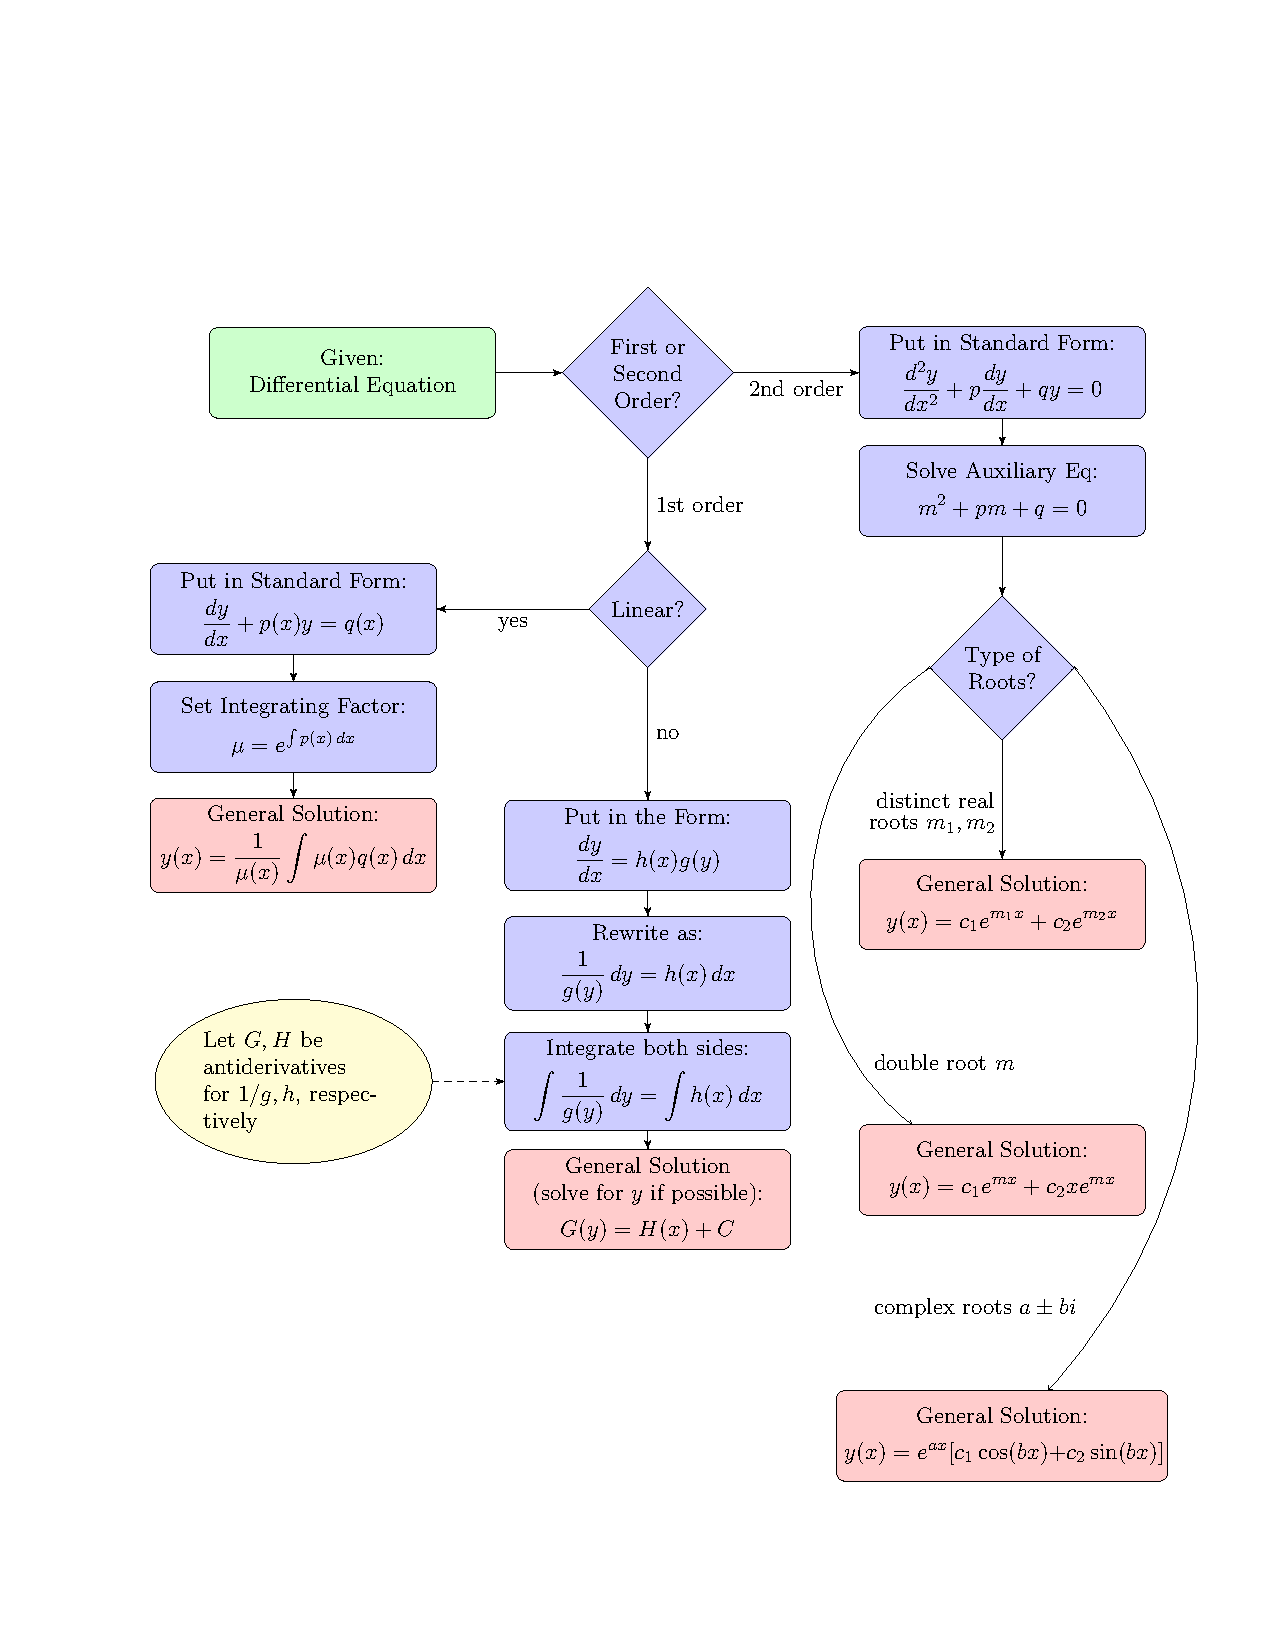
\includegraphics[width=\linewidth]{img/RevisionFlowchart}
	\caption{Flowchart for solving first and second order ODEs. \href{http://courses.enriqueareyan.com/files/math/M343\%20Introduction\%20to\%20Differential\%20Equations\%20I/Resources/DifferentialEquations-Flowchart.pdf}{Source}.}
	\label{fig:revisionflowchart}
\end{figure}

% https://matheducators.stackexchange.com/questions/16825/diagram-of-methods-to-solve-differential-equations

\section{Systems of First-Order Linear Equations}\label{sec:firstorder}

\subsection{Classification of Differential Equations}

\begin{definition}
	Given some independent real variables $x_1, x_2, \ldots, x_n$ and some real-valued functions $y_1(x_j), y_2(x_j), \ldots, y_p(x_j)$, a system of differential equations is a system of equations relating them involving the derivatives $\p_j y_r, \p_i\p_j y_s, \ldots$ of the dependent variables:\footnote{In this case, the notation $x_j$ is used as a shorthand for the vector $\xt = (x_1, x_2, \ldots, x_n)$. In other cases where $j$ is specified, $x_j$ can be used to indicate the $j$th component of $\xt$.}
	\[
		\mathcal{F}_s[y_r, \p_j y_r, \ldots, x_j] = 0, \quad s = 1, \ldots, p.
	\]
\end{definition}

In other words, a differential equation is simply an equation relating a function and its derivatives.

\begin{eg}
	Some examples of differential equations are:
	\begin{equation*}
	\begin{split}
		y'(x) = 0 \\
		\ddot{y}(t) - \omega^2 y(t) = 0 \\
		\begin{cases} \dot{x}_1(t) = x_2(t) \\ \dot{x}_2(t) = -\sin(x_1(t)) \end{cases} \\
		(\p_x y)^2 + \tanh{x}\p_z y = e^{2x+z}.
	\end{split}
	\end{equation*}
\end{eg}

Differential equations may depend on \textbf{parameters}, like the real parameter $\omega$ in the second example. It is important to distinguish them from the independent variables (such as $t$ in the same example). This is usually clear from the context, but the defining feature of a parameter is that the differential equation does not involve any derivatives with respect to it. Nonetheless, solutions of differential equations depend on the parameters, and understanding this parametric dependence is an important part of analysing differential equations.

\subsubsection{ODEs vs. PDEs}

\begin{definition}
	Given the two sets $\{x_1, x_2, \ldots, x_n\}$ and $\{y_1(x_j), y_2(x_j), \ldots, y_p(x_j)\}$:
	\begin{enumerate}
		\item If $n=1$ (i.e. there is only one independent variable), we have an Ordinary Differential Equation (ODE) containing only ordinary derivatives, e.g. $\ddot{y}(t) - \omega^2 y(t) = 0$. 
		\item If $n>1$ (i.e. more than one independent variable), we have a Partial Differential Equation (PDE) containing partial derivatives, e.g. $(\p_x y)^2 + \tanh{x}\p_z y = e^{2x+z}$.
	\end{enumerate}
	If there is more than equation involving functions and there derivatives, we have a system of ODEs or PDEs. For example,
	\[
		\begin{cases} \dot{x}_1(t) = x_2(t) \\ \dot{x}_2(t) = -\sin(x_1(t)) \end{cases}
	\]
	is a system of two ODEs, since there are two equations and one independent variable, $t$.
\end{definition}

\subsubsection{Linear vs. Non-linear}
	
Consider ODEs with a single function of one variable $y(x)$. By collecting all the $y$-dependent terms, we can write the ODE as a condition on a (possibly $x$-dependent) map $L$ acting on $y$,
\[
	L[y] = f
\]
for some real function $f$. For example, $y''(x) - xy(x) = x^2$ corresponds to $L[y] = f$ with $L \equiv \frac{d^2}{dx^2} - x$ and $f(x) = x^2$.

\begin{definition}
	We say and ODE is \textbf{linear} if the associated map $L$ is linear, i.e. if it satisfies the property
	\[
		L[a_1 y_1 + a_2 y_2] = a_1 L[y_1] + a_2 L[y_2] \quad \forall a_1,a_2 \in \R
	\]
	and for any pair of functions $y_1$, $y_2$.
\end{definition}

In simple terms, linear ODEs and PDEs are those where the dependent variables $y_i(x_j)$ appear linearly, i.e. raised to the power of one. For example, $y''(x) + x^2 y'(x) = e^{2x}$ is a linear ODE, while $y'(x) + y(x)^2 = -\sin{x}$ is non-linear as it contains the $y(x)^2$ term.

Differential equations are also classified by \textbf{order}. The order of a differential equation is simply the highest-order derivative that it contains. For example, $y'' - xy = x^2$ is a second-order ODE.


\subsection{Introduction to Systems of First-Order ODEs}

In a system of first-order differential equations, we generally consider the independent variable $t$ and a set of dependent variables $x_i(t)$, established and connected as follows:
\begin{equation}\label{eq:fosystem}
	x_i'(t) = F_i(x_1, x_2, \ldots, x_n, t), \quad i = 1, 2, \ldots, n
\end{equation}

A system is said to be \vb{autonomous} if $\p_t F_i = 0$ for all $i$ (in other words, the equations are independent of $t$).

\begin{theorem}[Existence and Uniqueness]
	Let the functions $F_1, \ldots, F_n$ and partial derivatives $\p_{x_1}F_1, \ldots, \p_{x_n}F_1, \ldots, \p_{x_1}F_n, \ldots, \p_{x_n}F_n$ be continuous in the region $R$ defined by $\alpha \leq t \leq \beta$, $\alpha_i \leq x_i \leq \beta_i$, $\forall i$. Then for each point $(t_0, x_1^0, \ldots, x_n^0) \in R$, there exists an interval $[t_0-h, t_0+h]$ in which there is a unique solution $x_1 = \phi_1(t), \ldots, x_n = \phi_n(t)$ of \Cref{eq:fosystem} satisfying the initial condition $\phi_i(t_0) = x_i^0 \,\, \forall i$.
\end{theorem}

It is often useful to transform a higher-order differential equation into a system of first-order ODEs.

\begin{eg}
	Write the differential equation $y''' + 2(y')^2 + 3ty = 0$ as a system of first-order ODEs.
	
	We define new variables $x_1$, $x_2$ and $x_3$, with
	\begin{align*}
		x_1(t) &= y \\
		x_2(t) &= y' \\
		x_3(t) &= y''
	\end{align*}
	then it is clear that
	\begin{align*}
		x_1' &= y' = x_2 \\
		x_2' &= y'' = x_3
	\end{align*}
	and also that
	\[
	x_3' = y''' = -2(y')^2 - 3ty = -2x_2^2 - 3t x_1. 
	\]
	Thus the original ODE may be written as the following system:
	\begin{align*}
		x_1' &= x_2 \\
		x_2' &= x_3 \\
		x_3' &= -2x_2^2 - 3t x_1.
	\end{align*}
\end{eg}

The general method for transforming an arbitrary $n$th order ODE $y^{(n)}(t) = F(y, y', \ldots, y^{(n-1)}, t)$ into a system of first-order ODEs is as follows:
\begin{enumerate}
	\item Define $n$ new independent variables $x_1 = y$, $x_2 = y'$, ... $x_n = y^{(n-1)}$.
	\item Take derivatives:
	\begin{align*}
		x_1' &= x_2 \\
		x_2' &= x_3 \\
		&\vdots \\
		x_{n-1}' &= x_n \\
		x_n' &= y^{(n)} = F(y, \ldots, y^{(n-1)}, t).
		\intertext{\item Hence the system is}
		x_1' &= x_2 \\
		&\vdots \\
		x_n' &= F(x_1, \ldots, x_{n-1}, t).
	\end{align*}
\end{enumerate}

\begin{exercise}
	Consider the second-order ODE with parametric dependence on $m, \gamma \in \R$:
	\[
		mu'' + \gamma u' + ky = F(t).
	\]
	Convert this into a system of first-order ODEs.
\end{exercise}

\subsubsection{Geometric Interpretation}

Geometrically, we may visualise a system of first-order equations as a vector field. If the system is autonomous, then the vector field will be static over time, while if the system is not autonomous then the vector field will change over time.

The solutions to the system are tangential to the vectors - in order words, the solution trajectories follow the arrows (see \Cref{fig:geomsys}).

\begin{figure}[!ht]
	\centering
	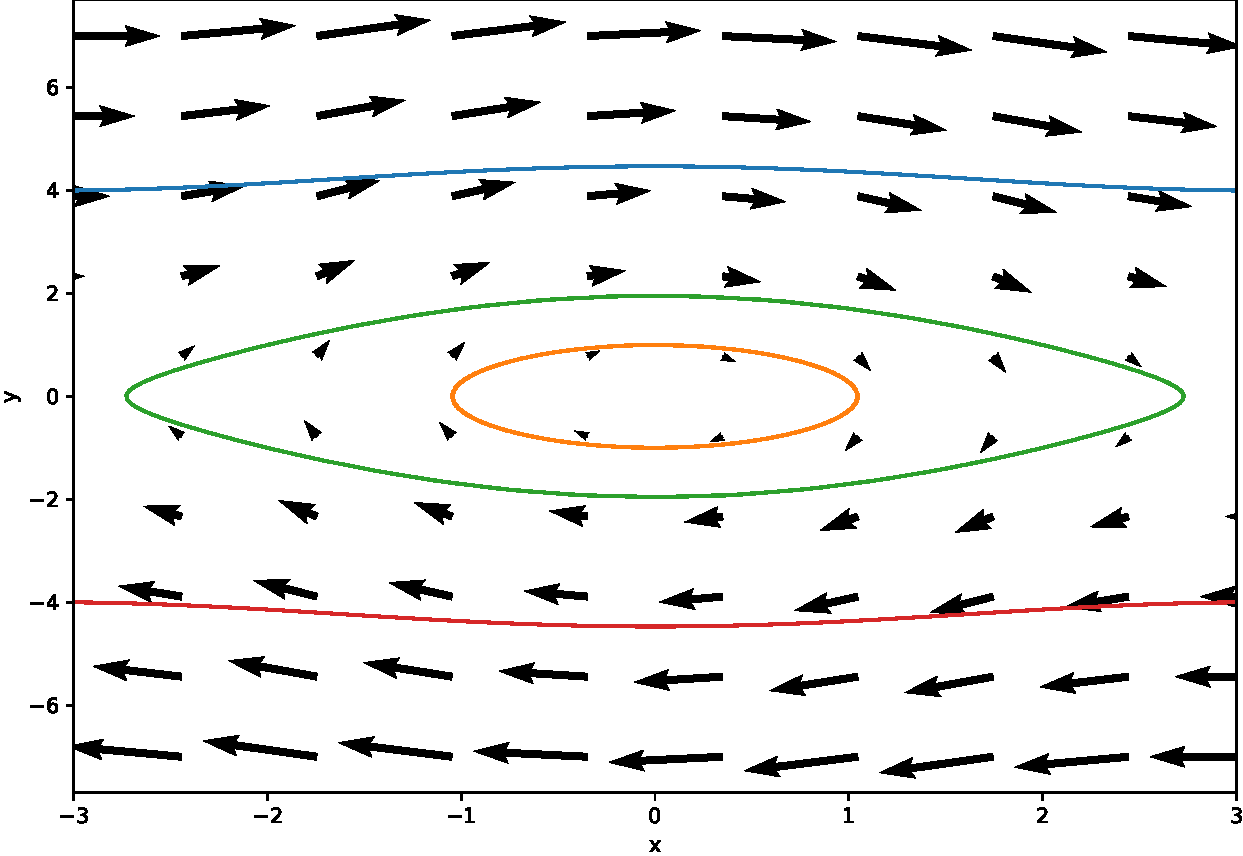
\includegraphics[width=0.7\textwidth]{vectorField.pdf}
	\caption{Direction field and selected solution trajectories for the system $x_0' = x_1$ and $x_1' = -\sin(x_0)$. Note that this is an example of an autonomous system.}
	\label{fig:geomsys}
\end{figure}


\subsection{Linear Systems of ODEs}

The general form of a linear system of ODEs is
\begin{equation}\label{eq:linearsystem}
	x_i'(t) = \sum_{j=1}^n P_{ij}(t) x_j(t) + g_i(t), \quad i = 1,\ldots,n.
\end{equation}

\begin{theorem}
	If $P_{ij}(t)$ and $g_i(t)$ are continuous in $[\alpha, \beta] \implies \exists t_0 \in (\alpha, \beta)$, there is a unique solution $x_t = \phi_i(t)$ in $[\alpha, \beta]$ solving \Cref{eq:linearsystem} and satisfying the initial condition $\phi_i(t_0) = x_i^0$.
\end{theorem}

For simplicity, we define the vector $\xt$ and matrix $P(t)$ as
\begin{equation}
	\xt = (x_1(t), x_2(t), \ldots, x_n(t)) \in \R^n \quad \text{and} \quad P(t) = \mat{P_{11}(t) & \cdots & P_{1n}(t) \\ \vdots & \ddots & \vdots \\ P_{n1}(t) & \cdots & P_{nn}(t)} \in \R^{n \times n}.
\end{equation}

Then \Cref{eq:linearsystem} may be written as
\begin{equation}\label{eq:linearsystemvector}
	\xtp = P(t) \xt + \gt.
\end{equation}

We say the system is homogeneous if $\vb{g} = \bm{0}$; otherwise, it is non-homogeneous or inhomogeneous. For now, we will only work with homogeneous systems, which we may write as $\vbx' = P\vbx$.

\begin{theorem}[Principle of Superposition]\label{thrm:superposition}
	If $\{\vbx^{(j)}(t)\}$, $j = 1, \ldots, p$ is a set of solutions,
	\begin{equation}\label{eq:gensol}
		\xt = \sum_{j=1}^p c_j \vbx^{(j)}(t), \quad c_j \in \R
	\end{equation}
	is also a solution.
\end{theorem}

\begin{proof}
	We have that $\vbx^{(j)}(t)$ is a solution of $\xtp = P(t) \xt$ (\Cref{eq:linearsystemvector}). Therefore
	\[
	\vbx^{(j)'}(t) = P(t) \vbx^{(j)}(t), \quad \forall j.
	\]
	Now, we find that
	\begin{align*}
		\xtp &= \sum_{j=1}^p c_j \vbx^{(j)'}(t)
		= \sum_{j=1}^p c_j P(t) \vbx^{(j)}(t) \\
		&= P(t) \sum_{j=1}^p c_j \vbx^{(j)}(t) \tag{Since $P(t)$ is indep. of $j$} \\
		&= P(t) \xt,
	\end{align*}
	i.e. $\xt$ satisfies the original ODE, making it a solution.
\end{proof}

\begin{remark}
	The Principle of Superposition only applies to homogeneous systems; that is, those of the form $\xtp = P\xt$.
\end{remark}

The space of solutions is a vector space of dimension $n$. To analyse the linear independence of $\{\vbx^{(j)}(t)\}, j = 1, \ldots, n$, we consider the following determinant
\begin{equation}\label{eq:wronskian}
	\det(\vbx^{(1)}(t), \vbx^{(2)}(t), \ldots, \vbx^{(n)}(t)) = \left| \begin{array}{cccc} x_1^{(1)} & x_1^{(2)} & \cdots & x_1^{(n)} \\ x_2^{(1)} & x_2^{(2)} & \cdots & x_2^{(n)} \\ \vdots & \vdots & \ddots & \vdots \\ x_n^{(1)} & x_n^{(2)} & \cdots & x_n^{(n)}
	\end{array} \right|
\end{equation}
Then, if this determinant is non-zero, the set of vectors are linearly independent. We call this determinant the \vb{Wronskian}, $W[\{\vbx^{(j)}(t)\}]$.

\begin{theorem}\label{thrm:fundamentalset}
	If $W[\{\vbx^{(j)}(t)\}] = W(t) \neq 0$ for $\alpha \leq t \leq \beta$, we say $\{\vbx^{(j)}(t)\}$ forms a fundamental set of solutions. Then, any solution may be written as a linear combination of the $\vbx^{(j)}$
	\[
	\xt = \sum_{j=1}^n c_j \vbx^{(j)}(t).
	\]
\end{theorem}

\begin{theorem}[Abel's Theorem]
	If $W(t_0) \neq 0$ for some $t_0$, then $W(t) \neq 0$ for all $\alpha \leq t \leq \beta$.
\end{theorem}

\begin{theorem}[Abel's Formula]
	The Wronskian satisfies
	\[
	W'(t) = \text{tr}(P(t)) W(t) = (P_{11} + \cdots + P_{nn}) W(t).
	\]
	Hence
	\[
	W(t) = e^{\int_{t_0}^t \text{tr} P(s) \,ds} W(t_0).
	\]
\end{theorem}

\begin{remark}
	Abel's Formula implies Abel's Theorem since if $W(t_0) \neq 0$, so too must $W(t) \neq 0$ since the exponential function is always non-zero.
\end{remark}

\begin{proof}
	We will use the definition of the derivative:
	\begin{equation}\label{eq:abelproof}
		W'(t) = \lim_{h\to 0} \frac{W(t+h) - W(t)}{h}.
	\end{equation}
	Note that the system of equations we are considering is homogeneous, i.e. $\xtp = P\xt$.
	
	Now we use the Taylor Expansion of $\vbx(t+h)$:
	\begin{align*}
		\vbx(t+h) &= \xt + h\xtp + O(h^2) \\
		&= \xt + hP(t)\xt + O(h^2) \tag{Using $\xtp = P\xt$} \\
		&= (I + hP(t))\xt + O(h^2)
	\end{align*}
	Then
	\begin{align*}
		W(t+h) &= \det\left(\vbx^{(1)}(t+h), \ldots, \vbx^{(n)}(t+h)\right) \\
		&= \det\left((I + hP(t))\vbx^{(1)}(t), \ldots, (I + hP(t))\vbx^{(n)}(t)\right) + O(h^2) \\
		&= \det\left[(I+hP(t))(\vbx^{(1)}(t), \ldots, \vbx^{(n)}(t))\right] + O(h^2) \\
		&= \det\left(I+hP(t)\right) \cdot \det\left(\vbx^{(1)}(t), \ldots, \vbx^{(n)}(t)\right) + O(h^2) \tag{Using $\det(AB) = \det(A)\det(B)$} \\
		&= \det\left(I+hP(t)\right) \cdot W(t) + O(h^2) \tag{By def. of Wronskian}
	\end{align*}
	
	Now looking at $\det\left(I+hP(t)\right)$:
	\begin{align*}
		\det\left(I+hP(t)\right) &= \left|\begin{array}{cccc}1+hP_{11} & hP_{12} & \cdots & hP_{1n} \\ hP_{21} & 1+hP_{22} & \cdots & hP_{2n} \\ \vdots & \vdots & \ddots & \vdots \\ hP_{n1} & hP_{n2} & \cdots & 1+hP_{nn} \\\end{array}\right| \\
		&= (1+hP_{11})\left|\begin{array}{cccc}hP_{12} & \cdots & hP_{1n} \\ \vdots & \ddots & \vdots \\hP_{n2} & \cdots & 1+hP_{nn} \\\end{array}\right| + O(h^2) \\
		&= (1+hP_{11})(1+hP_{22})\cdots (1+hP_{nn}) + O(h^2) \\
		&= 1 + hP_{11} + \cdots + hP_{nn} + O(h^2) \\
		&= 1 + h \text{tr}(P(t)) + O(h^2).
	\end{align*}
	Where all terms of the order $h^2$ or higher are collected under the umbrella of $O(h^2)$. Therefore
	\[
	W(t+h) = (1 + h \text{tr}(P(t))) W(t) + O(h^2)
	\]
	
	Finally, using this in \Cref{eq:abelproof}:
	\begin{align*}
		W'(t) &= \lim_{h\to 0} \frac{W(t+h) - W(t)}{h} \\
		&= \lim_{h\to 0} \frac{W(t) + h \text{tr}(P(t)) W(t) - W(t) + O(h^2)}{h} \\
		&= \lim_{h\to 0} \frac{h\text{tr}(P(t)) W(t)}{h} + \lim_{h\to 0}\frac{O(h^2)}{h} \\
		&= \text{tr}(P(t)) W(t).
	\end{align*}
	From which the formula for $W(t)$ follows easily.
\end{proof}

\subsection{Homogeneous Linear Systems with Constant Coefficients}\label{sec:homocc}

The aim of this section is to solve systems of $n$ first-order ODEs of the form $\xtp = A \xt$, $A \in \R^{n\times n}$, with $A$ a constant matrix.

To do this, we seek exponential solutions (similar to the method used for solving ODEs with constant coefficients in \Cref{sec:secondorderconst}); this is, those of the form
\begin{align*}
	\xt &= e^{rt} \xib \\
	\implies \xtp &= re^{rt} \xib = A e^{rt} \xib \\
	\implies (A-rI)\xib &= \bm{0}.
\end{align*}

In other words, we require that $r$ is an eigenvalue of $A$ and $\xib$ is the corresponding eigenvector. The $n$ eigenvalues then yield $n$ solutions to the system (if they all exist).\footnote{One might wonder how we come up with the idea for exponential solutions. We can derive this by starting with a simpler guess for the solutions of $\xt = f(t)\xib$ - simply a function of time multiplied by a constant vector $\xib$. Then we substitute this into the differential equation $\xtp = A \xt$ and obtain the equation
\[
	f'(t) \xib = f(t) A \xib \overset{f(t) \neq 0}{\implies} \frac{f'(t)}{f(t)}\xib = A\xib.
\]
Since there is no time-dependence on the right-hand side of this equation, $\frac{f'(t)}{f(t)}$ must be constant i.e. $\frac{f'(t)}{f(t)} = r$ and the equation above becomes $A\xib = r \xib$. We can then see that this is solved by $f(t) = e^{rt}$ and $\xib$ being an eigenvector of $A$ associated with the eigenvalue $r$. (Normally $f(t) = e^{rt}$ would contain an arbitrary constant $+C$, but since the eigenvector $\xib$ already contains an arbitrary constant of multiplication - $k\xib$ is also an eigenvector for $k \in \R \setminus \{0\}$ - 	there is no loss of generality by omitting the constant from $f(t)$.)}

Assuming the eigenvalues are all distinct, we have $n$ solutions, each of the form
\[
\vbx^{(j)}(t) = e^{r_j t} \xib_j, \quad j = 1, \ldots, n.
\]

We can see that these form a fundamental set, since
\begin{align*}
	W[\{\vbx^{(j)}(t)\}] &= \det(\vbx^{(1)}(t), \vbx^{(2)}(t), \ldots, \vbx^{(n)}(t)) \\
	&= \underbrace{e^{(r_1 + \cdots + r_n)t}}_{\neq 0} \det (\xib_1, \ldots, \xib_n)
\end{align*}
and $\det (\xib_1, \ldots, \xib_n) \neq 0$ since the eigenvectors associated with distinct eigenvalues are linearly independent. Therefore the Wronskian itself is non-zero, and we apply the result of \Cref{thrm:fundamentalset}.

Therefore the general solution may be written as
\begin{equation}\label{eq:generalsol}
	\xt = \sum_{j=1}^n c_j e^{r_jt} \xib_j.
\end{equation}

This holds provided that all eigenvalues are distinct ($r_i \neq r_j$ for $i \neq j$), \textbf{or} the algebraic multiplicity of each eigenvalue is equal to the geometric multiplicity.

\begin{eg}\label{eg:constsys1}
	Solve the system $\xtp = \mat{1 & 1 \\ 4 & 1} \xt$.
	
	We seek solutions of the form $\xt = e^{rt} \xib$, which as seen above requires that
	\begin{align*}
		(A-rI)\xib &= \bm{0} \\
		\implies \mat{1-r & 1 \\ 4 & 1-r} \xib &= \bm{0} \\
		\implies \det \mat{1-r & 1 \\ 4 & 1-r} &= 0 \\
		\implies (1-r)^2 -4 &= 0 \implies r = -1, 3.
	\end{align*}
	
	Now we find the eigenvectors associated with the eigenvalue $r_1=3$:
	\begin{align*}
		\mat{1-3 & 1 \\ 4 & 1-3} \xib = \mat{-2 & 1 \\ 4 & -2} \xib &= \bm{0} \\
		\implies \xib_1 &= \mat{1 \\ 2}.
	\end{align*}
	
	Similarly for $r_2=-1$:
	\begin{align*}
		\mat{1-(-1) & 1 \\ 4 & 1-(-1)} \xib = \mat{2 & 1 \\ 4 & 2} \xib &= \bm{0} \\
		\implies \xib_2 &= \mat{1 \\ -2}.
	\end{align*}
	
	Therefore the general solution may be written as
	\[
	\xt = c_1 e^{3t} \mat{1 \\ 2} + c_2 e^{-t} \mat{1 \\ -2}.
	\]
\end{eg}

\begin{remark}
	We can multiply through the vectors on the right-hand side of the general solution to write the equation as follows:
	\[
	\xt = \mat{x_1 \\ x_2} = \mat{c_1 e^{3t} + c_2 e^{-t} \\ 2c_1 e^{3t} - 2c_2 e^{-t}}.
	\]
\end{remark}

\begin{eg}
	Solve the system $\xtp = \mat{0 & 1 & 1 \\ 1 & 0 & 1 \\ 1 & 1 & 0} \xt$.
	
	As in \Cref{eg:constsys1}, we seek exponential solutions, and find the eigenvalues of the coefficient matrix to be $r_1 = -1$ and $r_2 = 2$. Note that the eigenvalue $r=-1$ has an algebraic multiplicity of 2.
	
	In finding eigenvectors, the eigenvector associated with $r=2$ is straightforward, with $\xib = \mat{1 \\ 1 \\ 1}$. For the eigenvalue $r=-1$, we find that the geometric multiplicity is 2, thus there are two linearly independent eigenvalues: $\xib = \mat{1 \\ 0 \\ -1}$ and $\xib = \mat{0 \\ 1 \\ -1}$.
	
	Putting this together, we may write the general solution as 
	\[
	\xt = c_1 e^{-t}\mat{1 \\ 0 \\ -1} + c_2 e^{-t} \mat{0 \\ 1 \\ -1} + c_3 e^{2t}\mat{1 \\ 1 \\ 1}.
	\]
\end{eg}

These two examples serve to illustrate the two different cases mentioned following \Cref{eq:generalsol} - where all eigenvalues are distinct or where algebraic and multiplicities are equal for all eigenvalues.

\begin{remark}
	With $\xt = \sum_{j=1}^n c_j e^{r_jt} \xib_j$, we may consider the behaviour of the solution as $t \to \infty$:
	\begin{itemize}
		\item $x \to 0$ if $\Re(r_j) < 0 \,\, \forall j$,
		\item $x \to \infty$ if $\Re(r_j) > 0 \,\, \forall j$,
		\item $x \to \infty$ for most initial conditions if $\exists j: \Re(r_j) > 0$.
	\end{itemize}
\end{remark}

\subsection{Homogeneous Linear Systems with Complex Eigenvalues}\label{sec:complexeigs}

In this section, we aim to solve the system $\xtp = A\xt$ with $A$ having complex conjugate eigenvalues. In addition, we will aim to write the solution in terms of real functions.\footnote{The methods of \Cref{sec:homocc} apply perfectly well to systems with complex eigenvalues; the only issue is that writing e.g. \[\xt = c_1 e^{-t/2 + it}\mat{1 \\ i} + c_2 e^{-t/2 - it}\mat{1 \\ -i}\] seems odd as a solution to a system given entirely in real numbers.}

First, observe that if $r_1 = \lambda + i\mu$ is an eigenvalue and $\xib_1$ is an eigenvector, so is $r_2 = r_i^* = \lambda - i\mu$, with $\xib_2 = \xib_1^*$.

So now we have two solutions: $\vbx_1(t) = e^{r_1t} \xib_1$ and $\vbx_2(t) = \vbx_1^*(t) = e^{r_1^*t} \xib_1^*$. Therefore in the $n=2$ case, the general solution of the whole system may be written as
\begin{equation*}\label{eq:complexgen}
	\xt = c_1 e^{r_1t} \xib_1 + c_2 e^{r_1^*t} \xib_1^*.
\end{equation*}

We wish to write the general solution in terms of real-valued functions instead of $\vbx_1(t)$ and $\vbx_1^*(t)$. We can do this by taking the two solutions to be the real and imaginary parts of $\vbx_1(t)$, since
\begin{equation*}
	\begin{alignedat}{2}
		\widetilde{\vbx}_1 &= \Re(\vbx_1(t)), \hspace{50pt} \widetilde{\vbx}_2 &&= \Im(\vbx_1(t)) \\
		&= \frac{x_1 + x_1^*}{2} &&= \frac{x_1 - x_1^*}{2i} \\
		&= \frac{x_1 + x_2}{2} &&= \frac{x_1 - x_2}{2i}
	\end{alignedat}
\end{equation*}
In other words, the real and imaginary parts of $\vbx_1(t)$ may be written as a linear combination of the two original solutions $\vbx_1(t)$ and $\vbx_2(t)$, thus are also a solution by the Principle of Superposition (\Cref{thrm:superposition}).

\begin{eg}
	Solve the system $\xtp = \mat{-\sfrac12 & 1 \\ -1 & -\sfrac12} \xt$, expressing your answer in terms of real functions.
	
	As before, we see exponential solutions of the form $\xt = e^{rt} \xib$, which requires that
	\begin{align*}
		\det \mat{-\frac12 -r & 1 \\ -1 & -\frac12 -r} &= 0 \\
		\implies \left(\frac12 + r\right)^2 + 1 &= 0 \\
		\implies r &= -\frac12 \pm i.
	\end{align*}
	
	We now find the eigenvector associated with the eigenvalue $r = -\frac12 + i$:
	\[
	\mat{-i & 1 \\ -1 & -i}\xib = 0 \implies \xib_1 = \mat{1 \\ i}.
	\]
	The eigenvector $\xib_2$ is the conjugate of $\xib_1$, so the general solution to the system is
	\[
	\xt = c_1 e^{-t/2 + it}\mat{1 \\ i} + c_2 e^{-t/2 - it}\mat{1 \\ -i}.
	\]
	
	However, we would rather use $\widetilde{\vbx}_1 = \Re(\vbx_1(t))$ and $\widetilde{\vbx}_2 = \Im(\vbx_1(t))$, so we write
	\begin{align*}
		\vbx_1(t) = e^{-t/2 + it}\mat{1 \\ i} &= e^{-t/2}(\cos t + i\sin t)\mat{1 \\ i} \\
		&= e^{-t/2}\mat{\cos t + i\sin t \\ i\cos t -\sin t}
	\end{align*}
	Taking the real and imaginary parts of this solution yields
	\[
	\widetilde{\vbx}_1 = e^{-t/2}\mat{\cos t \\ -\sin t} \quad\text{and}\quad \widetilde{\vbx}_2 = e^{-t/2}\mat{\sin t \\ \cos t}
	\]
	and a general solution of
	\[
	\xt = d_1 e^{-t/2}\mat{\cos t \\ -\sin t} + d_2 e^{-t/2}\mat{\sin t \\ \cos t}.
	\]
\end{eg}


\subsection{Matrix Methods}

\subsubsection{Fundamental Matrices}

\begin{definition}
	A fundamental matrix $\Psi(t)$ is an $n \times n$ matrix with fundamental solutions $\vbx^{(i)}$ as columns:
	\[
		\Psi(t) = (\vbx^{(1)}(t), \ldots, \vbx^{(n)}(t)) = \mat{x_1^{(1)} & x_1^{(2)} & \cdots & x_1^{(n)} \\ x_2^{(1)} & x_2^{(2)} & \cdots & x_2^{(n)} \\ \vdots & \vdots & \ddots & \vdots \\ x_n^{(1)} & x_n^{(2)} & \cdots & x_n^{(n)}}.
	\]
\end{definition}

Properties of the fundamental matrix:
\begin{itemize}
	\item $\det \Psi(t) = W(t) \neq 0$ because $\vbx^{(i)}$ form a fundamental set (see also \Cref{eq:wronskian}).
	\item{Considering the general solution in \Cref{eq:gensol},
		\begin{align*}
			\xt = \sum_{j=1}^p c_j \vbx^{(j)}(t) = (\vbx^{(1)}(t), \ldots, \vbx^{(n)}(t)) \mat{c_1 \\ \vdots \\ c_n} = \Psi(t) \bm{c}
		\end{align*}
		i.e. the general solution is given by the fundamental matrix multiplied by a vector of constants. Indeed, by \Cref{thrm:fundamentalset}, we have that \emph{any} solution may be written this way.}
	\item $\Psi'(t) = A \Psi(t)$ i.e. $\Psi(t)$ is a solution of the system of ODEs.
	\item $\xt = \Psi(t) \Psi^{-1}(t_0) \vbx_0$ solves $\xtp = A\xt$, with $\vbx(t_0) = \vbx_0$.
\end{itemize}

\begin{eg}\label{eg:fundamentalmatrix}
	Consider the system $\xtp = \mat{1 & 2 \\ 0 & 3} \xt$.
	
	We can easily solve the system (this is left as an exercise) to find the general solution to be
	\[
	\xt = c_1 e^t \mat{1 \\ 0} + c_2 e^{3t} \mat{1 \\ 1}
	\]
	Therefore the fundamental matrix is
	\[
	\Psi(t) = \mat{e^t & e^{3t} \\ 0 & e^{3t}}.
	\]
	Note that we can also check that $\Psi'(t) = A\Psi(t)$ (exercise!)
\end{eg}

It is important to note that the fundamental matrix of a system is \textbf{not} unique. Indeed, any matrix with its columns being linearly independent solutions to the system of ODEs is a valid fundamental matrix, e.g. $\mat{e^t & -3e^{3t} \\ 0 & -3e^{3t}}$ and $\mat{e^t & e^{3t}-2e^t \\ 0 & e^{3t}}$ for the system in the above example. This may be summarised in the statement that $\Psi(t) \cdot B$ is a fundamental matrix for constant matrix $B$.

\subsubsection{Matrix Exponentiation}

Recall that, for some scalar $a \in \R$, $e^a$ may be defined by power series:
\[
e^a = \sum_{k=0}^{\infty} \frac{a^k}{k!}.
\]

For a matrix $A$, we define $e^{At}$ analogously:
\[
e^{At} = \sum_{k=0}^{\infty} \frac{(At)^k}{k!} = I + At + \frac{A^2t^2}{2!} + \frac{A^3t^3}{3!} + \cdots
\]

Alternatively,
\[
	e^{At} = \lim_{n\to\infty} \left(I + \frac{1}{n}A\right)^n.
\]

Properties of $e^{At}$:
\begin{itemize}
	\item $e^{At} = I$ at $t=0$.
	\item $\frac{d}{dt}(e^{At}) = A e^{At}$, i.e. $e^{At} = \Psi(t)$ for $\Psi(0) = I$.\footnote{Checking this using the series definition of $e^{At}$ is a good exercise.}
	\item The solution of $\xtp = A\xt$ such that $\vbx(0) = \vbx_0$ is $\xt = e^{At} \vbx(0)$. This is because $\xt = \Psi(t) \Psi^{-1}(0) \vbx_0$ and $\Psi^{-1}(0) = I$ for $\Psi(t) = e^{At}$ since $e^{At} = I$ at $t=0$.
\end{itemize}

\begin{eg}
	Returning to the example in \Cref{eg:fundamentalmatrix}, we found that a fundamental matrix for the system $\xtp = \mat{1 & 2 \\ 0 & 3} \xt$ was $\Psi(t) = \mat{e^t & e^{3t} \\ 0 & e^{3t}}$.
	
	In order to have $e^{A\cdot 0} = I$, we require that
	\[
	e^{At} = \Psi(t) \Psi^{-1}(0).
	\]
	Determining $\Psi^{-1}(0)$:
	\[
	\Psi(0) = \mat{1 & 1 \\ 0 & 1} \implies \Psi^{-1}(0) = \mat{1 & -1 \\ 0 & 1}.
	\]
	Therefore
	\[
	e^{At} = \Psi(t) \Psi^{-1}(0) = \mat{e^t & e^{3t} \\ 0 & e^{3t}} \mat{1 & -1 \\ 0 & 1} = \mat{e^t & e^{3t}-e^t \\ 0 & e^{3t}}.
	\]
\end{eg}

\textbf{Summary:} A fundamental matrix is a matrix with its columns being linearly independent solutions to the system $\xtp = A\xt$. The matrix $e^{At}$ is a fundamental matrix, with the additional condition that $e^{At}$ is equal to the identity matrix when $t=0$.\footnote{3Blue1Brown has an excellent video relating to matrix exponentials and systems of differential equations that I would highly recommend: click \href{https://www.youtube.com/watch?v=O85OWBJ2ayo}{here}.}

\subsubsection{Matrix Exponentiation and Diagonalisation}\label{sec:diag}

Recall that the $n \times n$ matrix $A$ is diagonalisable if it has $n$ independent eigenvectors $\xib^{(i)}$, with $A \xib^{(i)} = r_i \xib^{(i)}$.

We construct a matrix with the eigenvectors as columns
\[
	T = \left(\xib ^{(1)}, \ldots, \xib ^{(n)}\right) = \mat{\xib_1^{(1)} & \xib_1^{(2)} & \cdots & \xib_1^{(n)} \\ \xib_2^{(1)} & \xib_2^{(2)} & \cdots & \xib_2^{(n)} \\ \vdots & \vdots & \ddots & \vdots \\ \xib_n^{(1)} & \xib_n^{(2)} & \cdots & \xib_n^{(n)}}.
\]
The Matrix $AT$ has columns equal to $A \xib^{(i)} = r_i \xib^{(i)}$, thus
\begin{align*}
	AT &= \mat{r_1\xib_1^{(1)} & \xib_1^{(2)} & \cdots & r_n\xib_1^{(n)} \\ r_1\xib_2^{(1)} & \xib_2^{(2)} & \cdots & r_n\xib_2^{(n)} \\ \vdots & \vdots & \ddots & \vdots \\ r_1\xib_n^{(1)} & \xib_n^{(2)} & \cdots & r_n\xib_n^{(n)}} = T \mat{r_1 & 0 & \cdots & 0 \\ 0 & r_2 & \cdots & 0 \\ \vdots & \vdots & \ddots & \vdots \\ 0 & 0 & \cdots & r_n} \\
	&= T \text{diag}(r_1, \ldots, r_n) \equiv TD \\
	&\implies D = T^{-1}AT.
\end{align*}

The relation $D = T^{-1}AT$ corresponds to a change of basis $\vbx = t\vb{y}$, which can be seen from the fact that
\[
	\vbx t\vb{y} \implies T \frac{d\vb{y}}{dt} = AT\vb{y} \implies \frac{d\vb{y}}{dt} = T^{-1}AT \vb{y} = D\vb{y}.
\]
The fundamental matrix of the system under the change of variables is
\[
	Q(t) = e^{Dt} = \text{diag}(e^{r_1t}, e^{r_2t}, \ldots, e^{r_nt}) = \mat{e^{r_1t} & 0 & \cdots & 0 \\ 0 & e^{r_2t} & \cdots & 0 \\ \vdots & \vdots & \ddots & \vdots \\ 0 & 0 & \cdots & e^{r_nt}}.
\]
Then the fundamental matrix in the original variables $\vbx$ is
\[
	\Psi(t) = TQ(t) = T \text{diag}(e^{r_1t}, e^{r_2t}, \ldots, e^{r_nt}),
\]
and the exponential matrix is
\[
	e^{At} = \Psi(t) \Psi^{-1}(0) = TQT^{-1} = T \text{diag}(e^{r_1t}, e^{r_2t}, \ldots, e^{r_nt}) T^{-1}.
\]

\begin{eg}
	Compute $e^{At}$ for $A = \mat{1 & 1 \\ 4 & 1}$.
	
	We can easily find the eigenvalues to be $r=-1,3$ and the corresponding eigenvectors to be $\mat{1 \\ -2}$ and $\mat{1 \\ 2}$.
	
	So
	\[
	T = \mat{1 & 1 \\ -2 & 2} \quad \text{and} \quad T^{-1} = \mat{\sfrac{1}{2} & \text{-}\sfrac{1}{4} \\ \sfrac{1}{2} & \sfrac{1}{4}}
	\]
	then
	\[
	e^{At} = Te^{Dt}T^{-1} = \mat{1 & 1 \\ -2 & 2} \mat{e^{-t} & 0 \\ 0 & e^{3t}} \mat{\sfrac{1}{2} & \text{-}\sfrac{1}{4} \\ \sfrac{1}{2} & \sfrac{1}{4}} = \mat{\frac12(e^{-t}+e^{3t}) & \frac14(e^{3t}-e^{-t}) \\ e^{3t}-e^{-t} & \frac12(e^{-t}+e^{3t})}
	\]
\end{eg}


\subsection{Homogeneous Linear Systems with Repeated Eigenvalues}\label{sec:repeatedeigs}

We will now solve systems $\xtp = A\xt$ where the matrix $A$ has repeated eigenvalues with geometric multiplicity less than algebraic multiplicity. This is best illustrated with an example:

\begin{eg}\label{eg:repeigs}
	Solve the system $\xtp = A\xt$ with $A = \mat{1 & -1 \\ 1 & 3}$.
	
	As usual, we try exponential solutions of the form $\xt = e^{rt}\xib$, and find the only eigenvalue of the matrix to be $r=2$ with algebraic multiplicity 2. Now to find the associated eigenvector(s):
	\[
	\mat{-1 & -1 \\ 1 & 1}\xib = 0 \implies \xib = \mat{1 \\ -1}.
	\]
	Therefore one solution is $\vbx^{(1)}(t) = e^{2t}\mat{1 \\ -1}$, but what is the other solution?
	
	For the second solution, we try
	\[
	\xt = te^{2t}\xib + e^{2t}\etab.
	\]
	Substituting this into the equation for the system, we get
	\[
	\xtp = e^{2t}\left[(2t+1)\xib + 2\etab\right] = A(te^{2t}\xib + e^{2t}\etab).
	\]
	Cancelling the $e^{2t}$ and comparing the coefficients of $t$:
	\[
	2\xib = A\xib \implies (A-2I) \xib = \bm{0}
	\]
	Which is precisely the eigenvalue problem we already solved. Now comparing the coefficients of $t^0$:
	\begin{align*}
		\xib + 2\etab = A\etab \implies (A-2I)\etab &= \xib \\ \mat{-1 & -1 \\ 1 & 1}\etab &= \mat{1 \\ -1} \\
		\etab &= \mat{-1 \\ 0} + k\mat{1 \\ -1}
	\end{align*}
	$\etab$ is known as a \vb{generalised eigenvector}. Observe that we may add any scalar multiple of the eigenvector $\xib$ to $\etab$ since $(A-2I)\xib = \bm{0}$ thus this addition will not affect the RHS of the equation $(A-2I)\etab = \xib$.
	
	We can now write the second solution as
	\[
	\vbx^{(2)}(t) = e^{2t}\left(t\mat{1 \\ -1} + \mat{-1 \\ 0} + k\mat{1 \\ -1}\right).
	\]
	Therefore the general solution is
	\[
	\xt = c_1 e^{2t}\mat{1 \\ -1} + c_2 e^{2t}\left(t\mat{1 \\ -1} + \mat{-1 \\ 0} + k\mat{1 \\ -1}\right).
	\]
	Note that without loss of generality, we can set $k=0$ since $c_2 k e^{2t}\mat{1 \\ -1}$ is just a multiple of the first term in the general solution. therefore a better general solution is
	\[
	\xt = c_1 e^{2t}\mat{1 \\ -1} + c_2 e^{2t}\left(t\mat{1 \\ -1} + \mat{-1 \\ 0}\right).
	\]
\end{eg}

\begin{exercise}
	Check that $\vbx^{(1)}(t)$ and $\vbx^{(2)}(t)$ form a fundamental set of solutions by calculating the Wronskian.
\end{exercise}

In general, the process for solving systems with repeated eigenvalues and too few eigenvectors is to construct the following independent solutions:
\begin{equation*}
	\begin{alignedat}{2}
		\vbx^{(1)}(t) &= \xib e^{rt} \qquad &&(A-rI)\xib = \bm{0} \\
		\vbx^{(2)}(t) &= (\xib t + \etab)e^{rt} \qquad && (A-rI)\etab = \xib \\
		\vbx^{(3)}(t) &= (\xib \frac{t^2}{2} + \etab t + \bm{\zeta})e^{rt} \qquad &&(A-rI)\bm{\zeta} = \etab \cdots
	\end{alignedat}
\end{equation*}

\subsubsection{Connection to Matrix Methods and Jordan Form}

Returning to the system in \Cref{eg:repeigs} and its general solution, we can find the fundamental matrix to be
\[
\Psi(t) = \mat{e^{2t} & (t-1)e^{2t} \\ -e^{2t} & -te^{2t}}.
\]
Then
\[
\Psi(0) = \mat{1 & -1 \\ -1 & 0}	\implies \Psi^{-1}(0) = \mat{0 & -1 \\ -1 & -1},
\]
so
\[
e^{At} = \Psi(t)\Psi^{-1}(0) = \mat{(1-t)e^{2t} & -te^{2t} \\ te^{2t} & (t+1)e^{2t}}.
\]

The Jordan form is an upper triangular matrix with the eigenvalues on its main diagonal, a diagonal consisting entirely of ones above the main diagonal (superdiagonal), and zero entries everywhere else:
\[
J_r = \mat{r & 1 \\ 0 & r}, \mat{r & 1 & 0 \\ 0 & r & 1 \\ 0 & 0 & r}, \cdots
\]

We illustrate some cases in which the Jordan form appears using $2 \times 2$ matrices, still using the system in \Cref{eg:repeigs}.

First, let
\[
T = (\xib, \etab) = \mat{1 & -1 \\ -1 & 0}.
\]
Then we find that
\[
T^{-1}AT = \mat{0 & -1 \\ -1 & -1} \mat{1 & -1 \\ 1 & 3} \mat{1 & -1 \\ -1 & 0} = \mat{2 & 1 \\ 0 & 2} = J_2.
\]

Now we shall compute $e^{J_rt}$. This is useful since $T^{-1}AT = J_r \implies e^{At} = Te^{J_rt}T^{-1}$. Note that $e^{A+B} = e^A e^B$ provided that $AB = BA$. We have
\[
J_r = \mat{r & 1 \\ 0 & r} = \mat{r & 0 \\ 0 & r} + \mat{0 & 1 \\ 0 & 0}
\]
Then
\[
e^{\mat{r & 0 \\ 0 & r}t} = \mat{e^{rt} & 0 \\ 0 & e^{rt}}
\]
and using the series definition of $e^{At}$,
\[
e^{\mat{0 & 1 \\ 0 & 0}t} = I + \mat{0 & t \\ 0 & 0} + \cancelto{0}{\frac12\mat{0 & t \\ 0 & 0}^2 + \cdots} = \mat{1 & t \\ 0 & 1}
\]
where higher powers are discarded since the matrix $\mat{0 & t \\ 0 & 0}$ is nilpotent.

So
\[
e^{J_rt} = \mat{e^{rt} & 0 \\ 0 & e^{rt}} \mat{1 & t \\ 0 & 1} = \mat{e^{rt} & te^{rt} \\ 0 & e^{rt}} = e^{rt} \mat{1 & t \\ 0 & 1}.
\]

In addition, a similar procedure may be used to find that, for a $3 \times 3$ Jordan form matrix $J_r$,\footnote{In fact, for the general $n \times n$ case, \[e^{Jt} = \mat{1 & t & t^2/2 & \dots & t^{n-1}/(n-1)! \\ 0 & 1 & t & \dots & t^{n-2}/(n-2)! \\ \vdots & \vdots & \vdots & \ddots & \vdots \\ 0 & 0 & 0 & \dots & 1}.\] The proof of this is of course left as an exercise.}
\[
e^{J_rt} = e^{rt} \mat{1 & t & \frac{t^2}{2} \\ 0 & 1 & t \\ 0 & 0 & 1}.
\]

% Note that a lot of the derivations/proofs present in the video lectures were not carried over to these notes. There was a very good reason for this - \sout{I really couldn't be bothered} it was decided that they were best left as an exercise to the reader.

\subsubsection{Two More Examples}

\begin{eg}
	Solve the system $\xtp = \mat{3 & 1 \\ -4 & -1}\xt$.
	
	Through the usual process, we find the eigenvalue to be $r=1$ with algebraic multiplicity 2, and the corresponding eigenvector to be $\xib = \mat{1 \\ -2}$ i.e. with geometric multiplicity 1.
	
	Therefore we try a second solution $\vbx^{(2)}(t) = e^t(t\xib + \etab)$. This leads to the generalised eigenvector problem
	\begin{align*}
		(A-I)\etab &= \xib \\
		\mat{2 & 1 \\ -4 & -2}\etab &= \mat{1 \\ -2} \\
		\etab &= \mat{\sfrac{1}{2} \\ 0} + k\mat{1 \\ -2}
	\end{align*}
	Taking $k=0$ in the second solution, we find the following general solution:
	\[
	\xt = c_1 e^t \mat{1 \\ -2} + c_2 e^t \left(t\mat{1 \\ -2} + \mat{\sfrac{1}{2} \\ 0}\right).
	\]
\end{eg}

\begin{eg}
	Solve the system $\xtp = \mat{5 & -3 & -2 \\ 8 & -5 & -4 \\ -4 & 3 & 3}\xt$.
	
	Through the usual methods, we find the only eigenvalue to be $r=1$ with algebraic multiplicity 3. Now looking for the eigenvectors:
	\[
	\mat{4 & -3 & -2 \\ 8 & -6 & -4 \\ -4 & 3 & 2}\xib = \bm{0}.
	\]
	The rows of this matrix are all multiples of one another, so in looking for eigenvalues $\xib = \mat{x \\ y \\z}$, the only constraint is that $4x-3y-2z = 0$. Setting $x=0$ and $y=0$ respectively, we can find two linearly independent eigenvectors to be $\xib^{(1)} = \mat{1 \\ 0 \\ 2}$ and $\xib^{(2)} = \mat{0 \\ 2 \\ -3}$.
	
	Therefore two independent solutions are
	\[
	\vbx^{(1)}(t) = e^t\mat{1 \\ 0 \\ 2} \quad \text{and} \quad \vbx^{(2)}(t) = e^t\mat{0 \\ 2 \\ -3}.
	\]
	
	We will now try and find a third solution of the form
	\[
	\vbx^{(3)}(t) = e^t\left(t\left(a\xib^{(1)} + b\xib^{(2)}\right) + \etab \right).
	\]
	Substituting this into the equation for the system:
	\[
	\vbx^{(3)}(t) = e^t\left[t\left(a\xib^{(1)} + b\xib^{(2)}\right) + \etab + a\xib^{(1)} + b\xib^{(2)}\right] = Ae^t\left(t\left(a\xib^{(1)} + b\xib^{(2)}\right) + \etab\right).
	\]
	Cancelling the $e^t$ and equating the terms in $t$:
	\[
	Ae^t\left(a\xib^{(1)} + b\xib^{(2)}\right) = a\xib^{(1)} + b\xib^{(2)},
	\]
	which is satisfied since $\xib^{(1)}$ and $\xib^{(2)}$ are eigenvectors with corresponding eigenvalue $r=1$.
	
	Now comparing the terms in $t^0$:
	\begin{align*}
		A\etab &= \etab + a\xib^{(1)} + b\xib^{(2)} \\
		\implies (A-I)\etab &= a\xib^{(1)} + b\xib^{(2)} \\
		\implies \mat{4 & -3 & -2 \\ 8 & -6 & -4 \\ -4 & 3 & 2}\etab &= a\mat{1 \\ 0 \\ 2} + b\mat{0 \\ 2 \\ -3} = \mat{a \\ 2b \\ 2a-3b}
	\end{align*}
	We can find a compatibility condition between the elements of the vector $\mat{a \\ 2b \\ 2a-3b}$ based on the relation between the rows of the matrix $\mat{4 & -3 & -2 \\ 8 & -6 & -4 \\ -4 & 3 & 2}$ I.e, the second row is twice the first row, so $2a = 2b \iff a=b$, and the third row is the negative of the first, so $3b-2a = a$. Taking for simplicity $a=b=1$,
	\begin{align*}
		\mat{4 & -3 & -2 \\ 8 & -6 & -4 \\ -4 & 3 & 2}\etab = \mat{1 \\ 2 \\ -1}
	\end{align*}
	With $\etab = \mat{x \\ y \\ z}$ this gives a condition that $4x-3y-2z = 1$, so setting $y=z=0$ and recalling that the generalised eigenvector may contain any scalar multiple of the original eigenvectors, we find that
	\[
	\etab = \mat{\sfrac{1}{4} \\ 0 \\ 0} + k\mat{1 \\ 0 \\ 2} + l\mat{0 \\ 2 \\ -3}, \quad k,l \in \R.
	\]
	Taking $k=l=0$, the simplest form of the general solution is
	\[
	\xt = c_1 e^t \mat{1 \\ 0 \\ 2} + c_2 e^t \mat{0 \\ 2 \\ -3} + c_3 e^t \mat{t + \sfrac{1}{4} \\ 2t \\ -t}.
	\]
\end{eg}


\subsection{Non-homogeneous Linear Systems}

In this section, we turn to the Non-homogeneous system:
\[
\xtp = P(t) \vbx + \gt
\]
where $P(t)$ is an $n \times n$ matrix and $\gt$ is the $n \times 1$ vector that makes the system non-homogeneous. The general solution of this system can be given by:
\begin{equation}
	\xt = \vbx_h(t) + \vbx_p(t)
\end{equation}

where $\vbx_h(t)$ is the general solution of the homogeneous system and $\vbx_p(t)$ is the particular solution of the non-homogeneous system. Note that this is essentially the same as when solving a single non-homogeneous ODE such as $y'' + 2y' + 5y = 2 e^t$.

Now, we aim to find the particular solution $\vbx_p(t)$ to the non-homogeneous system. We will mainly focus on systems $\xtp = A\xt + \gt$, i.e. those which have constant coefficients instead of a matrix $P(t)$ which is dependent on $t$. There are three methods to solve this:
\begin{itemize}
	\item Diagonalisation, for constant coefficients $P(t) = A$, any $\gt$.
	\item Method of undetermined coefficients, for constant coefficients $P(t) = A$, exponential-polynomial $\gt$.
	\item Variation of parameters for any $P(t)$, any $\gt$.
\end{itemize}


\subsubsection{Diagonalisation}

Consider systems of the form
\begin{equation}
	\xtp = A \xt + \gt
\end{equation} 
where A is an $n \times n$ diagonalisable constant matrix. Let
\[
T = \left(\xib ^{(1)}, \ldots, \xib ^{(n)}\right) \quad \text{and} \quad \vbx = T \bm{y}.
\]
Then we have,
\begin{align*}
	\vbx' = T \bm{y}' &= A \vbx + \gt \\
	\implies T \bm{y}' &= A T \bm{y} + \gt
\end{align*}
We multiply by $T^{-1}$ to get:
\begin{equation}\label{eq:diagdecoupled}
	\bm{y}' = T^{-1} A T \bm{y} + T^{-1} \gt
\end{equation}
By \Cref{sec:diag}, recall $T^{-1} A T = \text{diag}(r_1,\ldots,r_n) = R$. Then we obtain a system of uncoupled ODEs:
\[
{y_i}' = r_i y_i + h_i(t)
\]
where $\bm{h}(t) = T^{-1} \gt$. Rearranging the terms and multiplying by $e^{-r_i t}$ (i.e. solving the ODE by integrating factors):
\begin{equation}\label{eq:diagsol}
	\begin{alignedat}{1}
		e^{-r_i t}(y_i' - r_i y_i) &= h_i e^{-r_i t} \\
		\implies (e^{-r_i t} y_i)' &= h_i e^{-r_i t} \\
		\implies e^{-r_i t} y_i &= c_i + \int^t_{t_0} h_i(s) e^{-r_i s} \,ds \\
		\implies y_i(t) &= c_i e^{r_i t} + e^{r_i t} \int^t_{t_0} h_i e^{-r_i s} \,ds
	\end{alignedat} 
\end{equation}

The solution $\xt$ is obtained by multiplying the matrix $T$ with $\bm{y}(t)$, where each component of $\bm{y}$ is given by the last line of \Cref{eq:diagsol}. The first term $c_i e^{r_i t}$ gives the general solution of the homogeneous equation $\xtp = A\xt$, while the second term yields the particular solution of the non-homogeneous system.

\begin{eg}\label{eg:nonhom}
	Solve the system $\xtp = A \xt + \gt = \mat{-2 & 1 \\ 1 & -2} \xt + \mat{2 e^{-t} \\ 3t}$
	
	The homogeneous solution is given by: $\vbx_h(t) = e^{rt} \xib$. By solving to find the eigenvalues, we find that $r$ satisfies the equation:
	\[
	(r+2)^2 -1=0 \implies r_1 = -1, r_2 = -3
	\] 
	The eigenvector corresponding to $r_1 = -1$ is $\xib^{(1)} = \mat{1 \\ 1}$ and the eigenvector corresponding to $r_2 = -3$ is $\xib^{(2)} = \mat{1 \\ -1}$. 
	
	Hence,
	\[
	\vbx_h(t) = c_1 e^{-t} \mat{1 \\ 1} + c_2 e^{-3t} \mat{1 \\ -1}
	\]
	Now we calculate the particular solution. Consider the matrix
	\[
	T = \left(\xib^{(1)}, \ldots, \xib^{(n)}\right) = \mat{1 &1 \\ 1 &-1}
	\]
	and let $\vbx = T \bm{y}$.
	
	Note that 
	\[
	T^{-1} = -\frac{1}{2} \mat{-1 & -1 \\ -1 & 1} = \mat{\sfrac{1}{2} & \sfrac{1}{2} \\ \sfrac{1}{2} & -\sfrac{1}{2}}
	\] 
	and 
	\[
	T^{-1} A T = \emph{diag}(r_1,\ldots,r_n) = \mat{-1 & 0 \\0 & -3}. 
	\]
	By \Cref{eq:diagdecoupled}, we have,
	\[
	\bm{y}' = T^{-1} A T \bm{y} + T^{-1} \mat{2 e^{-t} \\ 3t} = \mat{-1 & 0 \\0 & -3} \bm{y} + \mat{e^{-t}+\frac{3}{2}t \\ e^{-t}-\frac{3}{2}t}
	\]
	Thus,
	\begin{align*}
		y_1' &= -y_1 + e^{-t} +\frac{3}{2}t \\
		y_2' &= -3y_2 + e^{-t} -\frac{3}{2}t
	\end{align*}
	We can solve for $y_1$ and $y_2$ using the method of integrating factors as follows:
	\begin{align*}
		y_1'+y_1 = e^{-t} +\frac{3}{2}t \implies (e^ty_1)' &= 1 + \frac{3}{2}te^t \\
		\implies e^ty_1 = c_1 + t + \frac{3}{2}(te^t - e^t)
	\end{align*}
	Multiplying by $e^{-t}$:
	\begin{align}
		y_1(t) &= c_1 e^{-t} + t e^{-t} + \frac{3}{2}(t-1) \\
		\intertext{Similarly,}
		y_2(t) &= c_2e^{-3t} + \frac{e^{-t}}{2} - \frac{t}{2} + \frac{1}{6}
	\end{align}
	Finally,
	\[
	\xt = T \bm{y}(t) = \mat{1 &1 \\ 1 &-1} \mat{c_1 e^{-t} + t e^{-t} + \frac{3}{2}(t-1) \\ c_2e^{-3t} + \frac{e^{-t}}{2} - \frac{t}{2} + \frac{1}{6}} = \mat{e^{-t}(d_1 + t) + t + c_2e^{-3t} - \frac{4}{3} \\ e^{-t}(d_2 + t) + 2t - c_2e^{-3t} - \frac{5}{3}}
	\]
	where $d_1 = c_1 + \frac{1}{2}$ and $d_2 = c_1 - \frac{1}{2}$.
\end{eg}

Now we consider the situation where the matrix $A$ is not diagonalisable.

In this case, we take $T = (\xib, \etab, \ldots)$. Then, $T^{-1}AT$ is in Jordan Form. For example,
\[
\textbf{y}'(t) = \mat{r & 1 \\0 & r} \textbf{y}(t) +\textbf{h}(t),
\]
where $\textbf{h}(t) = T^{-1}\textbf{g}(t)$.

This can still be solved as we have:
\begin{align*}
	y_1' &= r_1y_1 + y_2 + h_1 \\
	y_2' &= r_2y_2 + h_2
\end{align*}
The second equation involves only $y_2$ whereas the first equation involves both $y_1$ and $y_2$, so it is possible to first find $y_2$ and substitute $y_2$ into the first equation to then find $y_1$. In other words, while the new set of equations is not completely de-coupled, the structure is such that we can solve for all $y_i$ by backwards substitution.

\subsubsection{Method of Undetermined Coefficients}

This method works when we have to solve a system of ODEs of the form
\[
\xtp = P(t) \vbx + \gt
\] 
where $P(t)$ is a fixed matrix $A$ and $\gt$ is a product or sum of an exponential and polynomial function or a sum of such products.

To solve the ODE, try $\vbx_p(t)$ of the same form as $\gt$, i.e. exponentials and polynomials of the same degree as $\gt$ but with arbitrary coefficients in the polynomials. The coefficients are then determined by applying $\vbx_p(t)$ into the ODE and then comparing the coefficients of $t, t^0, $ etc. to find which coefficients satisfy the ODE.

\begin{remark}[Exception:] If $\gt = \bm{c} e^{rt}$, where $r$ is an eigenvalue of A with algebraic multiplicity $n$, then try:
	\[
	\vbx_p(t) = (\bm{a}_n t^n+\bm{a}_{n-1} t^{n-1} + \cdots + \bm{a}_0)e^{rt}
	\]
\end{remark}

\begin{eg}\label{eg:nonhom2}
	We solve the same system as in \Cref{eg:nonhom}:
	\[ 
	\xtp = A\vbx + \gt = \mat{-2&1\\1&-2} \vbx + \mat{2e^{-t}\\3t}
	\]
	In \Cref{eg:nonhom}, we found that the eigenvalues of A are $r_1 = -1$ and $r_2 = -3$ with corresponding eigenvectors $\xib^{(1)} = \mat{1 \\ 1}$ and $\xib^{(2)} = \mat{1 \\ -1}$. Thus the homogeneous solution of the system is
	\[
	\vbx_h(t) = c_1e^{-t} \mat{1\\1} + c_2e^{-3t} \mat{1\\-1}
	\]
	Now, write
	\begin{equation}
		\gt = \mat{2e^{-t}\\3t} = \mat{0\\3t} +\mat{2e^{-t}\\0}
	\end{equation}
	Let $\vbx_p(t) = \vbx_p^{(1)}(t) + \vbx_p^{(2)}(t)$, where: $\vbx_p^{(1)}(t)$ is the trial function for $\mat{0\\3t}$ and $\vbx_p^{(2)}(t)$is the trial function for $\mat{2e^{-t}\\0}$.
	
	For $\vbx_p^{(1)}(t)$ we know it must solve
	\[
	\vbx_p^{(1)\prime} = \mat{-2&1\\1&-2}\vbx_p^{(1)} + \mat{0\\3t}.
	\]
	Here, we have a polynomial function but no exponential. This is equivalent to having an exponential function $e^{0t}$, but since 0 is not an eigenvalue of $A$, we need not follow the exception rule.
	
	So, let $\vbx_p^{(1)}(t) = \bm{a}t + \bm{b}$. Then 
	\[ 
	\vbx_p^{(1)\prime} = \bm{a} = \mat{-2&1\\1&-2}(\bm{a}t + \bm{b}) + \mat{0\\3t}
	\]
	Comparing the coefficients of $t$:
	\[
	\bm{0} = \mat{-2&1\\1&-2} \bm{a} + \mat{0\\3} \implies \mat{-2&1\\1&-2} \bm{a} = \mat{0\\-3}
	\]
	\[
	\begin{cases}
		-2a_1 + a_2 = 0 \\
		a_1 -2a_2 = -3
	\end{cases}
	\implies \bm{a} = \mat{1\\2}
	\]
	Comparing the coefficients of $t^0$ (i.e. constant terms): 
	\[
	\bm{a} = \mat{-2&1\\1&-2} \bm{b} = \mat{1\\2} \\
	\implies \begin{cases}
		-2b_1 + b_2 = 1 \\
		b_1 -2b_2 = 2
	\end{cases}
	\implies \bm{b} = -\mat{\sfrac43 \\ \sfrac53}
	\]
	Hence, 
	\[
	\vbx_p^{(1)}(t) = t\mat{1\\2} - \frac{1}{3}\mat{4\\5}
	\]
	For $\vbx_p^{(2)}(t)$ which solves 
	\begin{equation}\label{eq1.7.8}
		\vbx_p^{(2)\prime} = \mat{-2&1 \\ 1&-2}\vbx_p^{(2)}(t) + \mat{2e^{-t} \\ 0}
	\end{equation}
	$\gt$ has an exponential $e^{kt}$ where $k =-1$. $r_1 = -1$ is an eigenvalue of $A$, so we have to use the exception rule above. Since algebraic multiplicity of $r_1$ is 1, we try:
	\[
	\vbx_p^{(2)}(t) = (\bm{c}t + \bm{d})e^{-t}
	\]
	Substituting $\vbx_p^{(2)}$ into \Cref{eq1.7.8}:
	\[
	(-\bm{c}t - \bm{d} + \bm{c}) e^{-t} = \mat{-2&1 \\ 1&-2}(\bm{c}t + \bm{d})e^{-t} + \mat{2e^{-t}\\0}
	\]
	Comparing coefficients of $t$:
	\begin{equation}\label{eq:nonhomc}
		\begin{alignedat}{1}
			-\bm{c} = A\bm{c} \implies (A + I)\bm{c} &= \bm{0} \\
			\implies (A - r_1I) \bm{c} &= \bm{0}
		\end{alignedat}
	\end{equation}
	As solved before, $\bm{c} = \xib^{(1)} = \alpha
	\mat{ 1\\1}$. The $\alpha$ is introduced in the equation for $\bm{c}$ should not be fixed since there are many solutions to \Cref{eq:nonhomc}. They are all multiples of $\xib^{(1)}$ so $\alpha$ gives us the freedom to choose which multiple of $\xib^{(1)}$ we want.
	
	Now, comparing the coefficients of $t^0$:
	\[
	\bm{c} - \bm{d} = A\bm{d} + \mat{2\\0}
	\implies \bm{c} - \mat{2\\0} = \left(\mat{-2&1 \\ 1&-2} + I\right)\bm{d} = \mat{\alpha-2\\\alpha}
	\]
	Let $\mat{-1&1 \\ 1&-1}\bm{d} =B$. Then the rows of $B$ are multiples of each other so it is a singular matrix. So, the system is compatible only if $\alpha = -(\alpha - 2) \implies \alpha = 1$. Therefore,
	\[
	\mat{-1&1 \\ 1&-1}\bm{d} = \mat{-1\\1} \implies \bm{d} = \mat{1\\0} + k\mat{1\\1}
	\]
	So,
	\[\vbx_p^{(2)}(t) = e^{-t}\left(\mat{1\\1} + \mat{1\\0} + k\mat{1\\1}\right)
	\]
	Hence, 
	\[
	\vbx_p(t) = \vbx_p^{(1)}(t) + \vbx_p^{(2)}(t) = t\mat{1\\2} - \frac{1}{3}\mat{4\\5} + e^{-t}\left(t\mat{1\\1} + \mat{1\\0} + k\mat{1\\1}\right)
	\]
	However, note that the term $e^{-t}k\mat{1\\1}$ would get dissolved into the homogeneous solution since $\mat{1\\1}$ is an eigenvector for $r_1 = -1$, so we have the general solution to the ODE given by:
	\[
	\xt = \vbx_h(t) + \vbx_p(t) = c_1e^{-t}\mat{1\\1} + c_2e^{-3t}\mat{1\\-1} + t\mat{1\\2} - \frac{1}{3}\mat{4\\5} + e^{-t}\left(t\mat{1\\1} + \mat{1\\0} \right)
	\]
\end{eg}


\subsubsection{Variation of Parameters}

This method solves systems of the form: 
\begin{equation}\label{eq1.7.10}
	\xtp = P(t)\vbx + \gt
\end{equation}
where $P(t)$ is any matrix dependent on or independent of time and $\gt$ is any function of $t$.

Suppose we know that $\Psi(t)$ is a fundamental matrix for the system, then $\vbx_h(t) = \Psi(t)\bm{c}$ where $\bm{c}$ is a vector of parameters which parametrise the homogeneous solution.

Take $\vbx_p(t) = \Psi(t) \bm{u}(t)$. Substitute $\vbx_p$ into \Cref{eq1.7.10}. Then,
\[
\Psi' \bm{u} + \Psi \bm{u}' = P\Psi \bm{u} + \gt
\]
But we know that $\Psi' = P\Psi$, hence $\Psi'\bm{u}$ and $P\Psi\bm{u}$ cancel. Now,
\begin{equation}\label{eq:varparamu}
	\Psi \bm{u}' = \gt \implies \bm{u}' = \Psi^{-1}(t) \gt
\end{equation}
By integrating, 
\[
\bm{u}(t) = \bm{k} + \int_{t_0}^t \Psi^{-1}(s) \vb{g}(s)\,ds
\]
Multiply by $\Psi(t)$:
\begin{equation}\label{eq:varparam}
	\xt = \Psi(t)\bm{k} + \Psi(t) \int_{t_0}^t \Psi^{-1}(s) \vb{g}(s)\,ds
\end{equation}
Particularly for $\vbx(t_0) = \vbx_0$:
\begin{equation}
	\xt = \Psi(t) \Psi^{-1}(0) \vbx_0 + \Psi(t) \int_{t_0}^t \Psi^{-1}(s) \vb{g}(s)\,ds
\end{equation}

\begin{remark}
	Note that \Cref{eq:varparam} contains both the homogeneous solution and the particular solution, since $\Psi(t) \bm{k}$ corresponds to $\vbx_h(t)$ - the only difference is the letter used to denote the vector of arbitrary constants.
\end{remark}

\begin{remark}
	Note that we can go from the \Cref{eq:varparamu} to a solution in another way than explicitly finding $\Psi^{-1}$. Instead, we can write $\bm{u} = \mat{u_1' \\ \vdots \\ u_n'}$ then perform the multiplication $\Psi \bm{u}'$ and equate with $\gt$ to find a system of $n$ ODEs for $u_1', \dots, u_n'$. Algebraic manipulation may then be used to, for example, solve for $u_n'$ and then $u_n$ and back substitute to solve for the other components of $\bm{u}'$ and hence $\bm{u}$. An example of this method is given in \Cref{eg:varparamsolve}.
\end{remark}

\begin{eg}
	We solve the same system as in Examples \ref{eg:nonhom} and \ref{eg:nonhom2} using variation of parameters. A reminder that the system is
	\[
	\xtp = A\vbx + \gt = \mat{-2&1\\1&-2} \vbx + \mat{2e^{-t}\\3t}.
	\]
	We already know that the fundamental matrix $\Psi(t)$ is given by
	\[
	\Psi(t) = \mat{e^{-t} & e^{-3t} \\ e^{-t} & -e^{-3t}} \quad \text{with} \quad \Psi^{-1}(t) = \frac12 \mat{e^t & e^t \\ e^{3t} & -e^{3t}}.
	\]
	Then
	\begin{align*}
		\int \Psi^{-1}(t) \vb{g}(t) \,dt &= \frac12 \int \mat{e^t & e^t \\ e^{3t} & -e^{3t}} \mat{2e^{-t}\\3t} dt \\
		&= \frac12 \int \mat{2 + 3te^t \\ 2e^{2t} - 3te^{3t}} dt \\
		&= \frac12 \mat{2t + 3te^t - 3e^t \\ e^{2t} - te^{3t} + \frac13 e^{3t}}.
	\end{align*}
	Therefore we have the particular solution
	\begin{align*}
		\Psi(t) \int \Psi^{-1}(t) \vb{g}(t) \,dt &= \frac12 \mat{e^{-t} & e^{-3t} \\ e^{-t} & -e^{-3t}} \mat{2t + 3te^t - 3e^t \\ e^{2t} - te^{3t} + \frac13 e^{3t}} \\
		&= \frac12 \mat{2te^{-t} + 3t-3+e^{-t} + \frac13 - t \\ 2te^{-t} + 3t - 3 - e^{-t} + t - \frac13} \\
		&= t\mat{1\\2} + te^{-t}\mat{1\\1} + \frac12e^{-t}\mat{1\\-1} + \mat{-\sfrac{4}{3} \\ -\sfrac{5}{3}}.
	\end{align*}
	Then all that remains is to add in the homogeneous solution $\Psi(t) \bm{k}$:
	\[
	\xt = c_1e^{-t}\mat{1\\1} + c_2e^{-3t}\mat{1\\-1} + t\mat{1\\2} + te^{-t}\mat{1\\1} + \frac12e^{-t}\mat{1\\-1} + \mat{-\sfrac{4}{3} \\ -\sfrac{5}{3}}.
	\]
\end{eg}

\begin{eg}\label{eg:varparamsolve}
	Solve the system $\xtp = \mat{2 & -5 \\ 1 & -2}\xt + \mat{0\\\cos t}$.
	
	Through the usual method of searching for exponential solutions, we can find a fundamental matrix (in terms of real functions) to be
	\[
	\Psi(t) = \mat{5\cos t & 5\sin t \\ 2\cos t + \sin t & 2\sin t - \cos t}
	\]
	Then as in \Cref{eq:varparamu}, we must solve the equation 
	\[
	\Psi \bm{u}' = \gt = \mat{0 \\ \cos t} \quad \text{with} \quad \textbf{u}' = \mat{u_1' \\ u_2'}
	\]
	Performing this multiplication, we find the following two equations:
	\begin{align*}
		5\cos t u_1' + 5\sin t u_2' &= 0 \\ 
		2\cos t u_1' + \sin t u_1' + 2\sin t u_2' - \cos t u_2' &= \cos t
	\end{align*}
	The first equation clearly simplifies to 
	\begin{equation}\label{eq:varparameg2}
		\cos t u_1' + \sin t u_2' = 0.
	\end{equation}
	Then in the second equation, the $2\cos t u_1' + 2\sin t u_2'$ part equals zero by the first equation, so we have
	\[
	\sin t u_1' - \cos t u_2' = \cos t
	\]
	Multiplying through by $-\cos t$ and using the fact that from the first equation, $\cos t u_1' = -\sin t u_2'$ gives
	\[
	\sin^2t u_2' + \cos^2t u_2' = -\cos^2t,
	\]
	and using $\sin^2t + \cos^2t = 1$ gives the equation 
	\[
	u_2' = \frac{du_2}{dt} = -\cos^2t
	\] 
	This can be solved by simply integrating both sides, and using the fact that the integral of $\cos^2t$ is $\frac{t}{2} + \frac{\sin(2t)}{4} + C$\footnote{since we can write $\cos^2t = \frac12(1 + \cos(2t))$.} to give
	\[
	u_2 = k_1 - \frac{t}{2} - \frac14\sin(2t).
	\]
	Now returning to \Cref{eq:varparameg2}
	\begin{align*}
		\cos t u_1' + \sin t u_2' &= 0 \\
		\cos t u_1' - \sin t \cos^2t &= 0 \\
		u_1' &= \sin t \cos t \\
		\implies u_1 &= \frac12 \sin^2 t + k_2
	\end{align*}
	Finally, we find the particular solution $\xt$ by
	\begin{align*}
		\xt &= \Psi \bm{u} = \mat{5\cos t & 5\sin t \\ 2\cos t + \sin t & 2\sin t - \cos t} \mat{\frac12 \sin^2 t + k_2 \\ k_1 - \frac{t}{2} - \frac14\sin(2t)} \\
		&= \left(\frac12 \sin^2t + k_2\right)\mat{5\cos t \\ 2\cos t + \sin t} + \left(k_1 - \frac{t}{2} - \frac14\sin(2t)\right)\mat{5\sin t \\ 2\sin t - \cos t}.
	\end{align*}
	In fact, since $k_1$ and $k_2$ are arbitrary constants, this expression constitutes the entire general solution.
\end{eg}

\begin{eg}
	To illustrate the process for solving a system where the matrix $P(t)$ is not a constant matrix, we solve the system
	\[
	\xtp = \mat{0 & t^{-1} \\ t^{-1} & 0}\xt + \mat{te^t \\ 0},
	\]
	given that the solution to the homogeneous equation is
	\[
	\xt = c_1t\mat{1\\1} + c_2t^{-1}\mat{1\\-1}.
	\]
	From here, we find the fundamental matrix and its inverse:
	\[
	\Psi(t) = \mat{t & t^{-1} \\ t & -t^{-1}} \quad\text{with}\quad \Psi^{-1}(t) = -\frac12\mat{-t^{-1} & -t^{-1} \\ -t & t} = \frac12\mat{t^{-1} & t^{-1} \\ t & -t}
	\]
	Then
	\begin{align*}
		\int \Psi^{-1}(t)\gt \,dt &= \frac12 \int \mat{t^{-1} & t^{-1} \\ t & -t}\mat{te^t \\ 0} dt \\
		&= \frac12 \int\mat{e^t \\ t^2e^t}dt \\
		&= \frac12 \mat{e^t \\ e^t(t^2 - 2t + 2)}.
		\intertext{And the particular solution is}
		\Psi(t)\int \Psi^{-1}(t)\gt \,dt &= \frac12 \mat{t & t^{-1} \\ t & -t^{-1}} \mat{e^t \\ e^t(t^2 - 2t + 2)} \\
		&= \frac{e^t}{2}\mat{t+t-2+2t^{-1} \\ t-t+2-2t^{-1}} \\
		&= e^t\mat{t - 1 + t^{-1} \\ 1 - t^{-1}}.
	\end{align*}
	So the general solution is
	\[
	\xt = c_1t\mat{1\\1} +c_2 t^{-1}\mat{1\\-1} + e^t\mat{t - 1 + t^{-1} \\ 1 - t^{-1}}
	\]
\end{eg}

\begin{remark}
	If $P(t) = A$, then $e^{At} = \Psi(t) \Psi^{-1}(0)$, so:
	\[
	\xt = e^{At} \vbx_0 + e^{At} \int_{t_0}^t e^{-As} \vb{g}(s)\,ds
	\]
\end{remark}

\pagebreak
\subsection{Summary}

The general method for transforming an arbitrary $n$th order ODE $y^{(n)}(t) = F(y, y', \ldots, y^{(n-1)}, t)$ into a system of first-order ODEs is as follows:
\begin{enumerate}
	\item Define $n$ new independent variables $x_1 = y$, $x_2 = y'$, $\ldots$, $x_n = y^{(n-1)}$.
	\item{Take derivatives: $x_1' = x_2$, $x_2' = x_3$, $\ldots$, $x_{n-1}' = x_n$, $x_n' = y^{(n)} = F(y, \ldots, y^{(n-1)}, t)$.}
	\item{Hence the system is $x_1' = x_2$, $\ldots$, $x_n' = F(x_1, \ldots, x_{n-1}, t)$.}
\end{enumerate}

We mainly solve systems of ODEs with constant coefficients, written in the form $\xtp = A\xt$. To do this, we find eigenvalues $r_i$ and corresponding eigenvectors $\xib_i$ of the matrix $A$. Then the general solution may be written as
\[
\xt = \sum_{j=1}^n c_j e^{r_jt} \xib_j.
\]
This holds provided that all eigenvalues are distinct ($r_i \neq r_j$ for $i \neq j$), \textbf{or} the algebraic multiplicity of each eigenvalue is equal to the geometric multiplicity.

In the case that we get complex eigenvalues in complex conjugate pairs,\footnote{Complex eigenvalues will always come in conjugate pairs when $A$ is a real matrix.} then we first find one solution in terms of complex function
\[
\vbx^{(1)}(t) = e^{r_1t}\xib_1, \quad r_1 \in \C, \,\,\xib_1 \in \C^n.
\]
To write the solution in terms of real functions, two linearly independent solutions are found by taking only the real and imaginary part of $\vbx^{(1)}(t)$:
\[
\widetilde{\vbx}_1 = \Re(\vbx^{(1)}(t)), \quad \text{and} \quad \widetilde{\vbx}_2 = \Im(\vbx^{(1)}(t))
\]

The fundamental matrix
\[
\Psi(t) = (\vbx^{(1)}(t), \dots, \vbx^{(n)}(t))
\]
satisfies the matrix ODE $\Psi' = A\Psi$. Then the general solution is
\[
\xt = \Psi(t) \bm{c}, \quad, \bm{c} = \mat{c_1 \\ c_n}.
\]
The exponential matrix $e^{At}$ is that for which
\[
\left(e^{At}\right)' = Ae^{At} \quad \text{and} \quad e^{At} = I.
\]
$e^{At}$ can be obtained as
\begin{itemize}
	\item $e^{At} = \Psi(t)\Psi^{-1}(0)$.
	\item $e^{At} = \sum_{k=0}^{\infty} \frac{(At)^k}{k!}$.
	\item $e^{At} = T \text{diag}(e^{r_1t}, \dots, e^{r_nt})T^{-1}$ for diagonalisable $A$ with $T^{-1}AT = \text{diag}(r_1, \dots, r_n)$.
\end{itemize}

\begin{remark}
	Note that $e^Ae^B \neq e^{A+B}$ in general (unless $AB = BA$).
\end{remark}

Solutions of $\xtp = A\xt$ for constant matrix $A$ and with repeated eigenvalues have the form
\begin{equation*}
	\begin{alignedat}{2}
		\vbx^{(1)}(t) &= \xib e^{rt} \qquad &&(A-rI)\xib = \bm{0} \\
		\vbx^{(2)}(t) &= (\xib t + \etab)e^{rt} \qquad && (A-rI)\etab = \xib \\
		\vbx^{(3)}(t) &= (\xib \frac{t^2}{2} + \etab t + \bm{\zeta})e^{rt} \qquad &&(A-rI)\bm{\zeta} = \etab \cdots
	\end{alignedat}
\end{equation*}

Correspondingly, the similarity matrix $T = (\xib, \etab, \dots)$ gives the Jordan form
\[
T^{-1}AT = J_r = \mat{r & 1 \\ 0 & r}, \mat{r & 1 & 0 \\ 0 & r & 1 \\ 0 & 0 & r}, \cdots
\]

For an non-homogeneous system of the form $\xtp = P(t)\xt + \gt$, the general solution is the sum of the homogeneous solution and the particular solution: $\xt = \vbx_h(t) + \vbx_p(t)$.

There are three techniques to find the particular solution:
\begin{enumerate}
	\item Diagonalisation, for constant matrix $P(t)=A$ and any $\gt$. This uses a change of variables $\vbx = T\bm{y}$, with $T = (\xib ^{(1)}, \ldots, \xib ^{(n)})$, leading to a system of uncoupled ODEs which may be solved individually, often using integrating factors.
	\item Method of undetermined coefficients, for constant coefficients $P(t)=A$ and exponential-polynomial $\gt$. A trial solution is used based on the form of $\gt$, then substituted into the original system. Coefficients of $t$, $t^0$ etc. are compared to solve for the undetermined coefficients.
	\item Variation of parameters, for any $P(t)$ and $\gt$. Given a fundamental matrix $\Psi(t)$, the solution $\xt$ is given by $\xt = \Psi(t)\bm{k} + \Psi(t) \int \Psi^{-1}(s) \vb{g}(s)\,ds$.
\end{enumerate}

\vfill
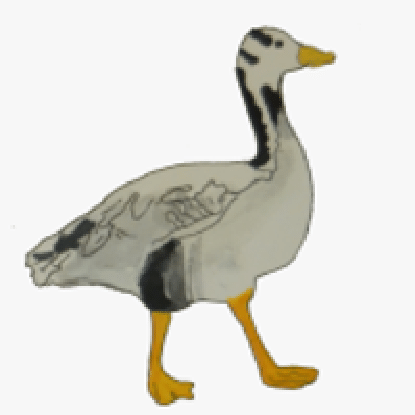
\includegraphics[width=3cm]{duck.png}
\tikz[remember picture,overlay]{\node[ellipse callout, draw, thick, fill=white, overlay, callout absolute pointer={($(-0.4,2.5)$)}] at ($(3.5,3.5)$) {\Large{I am a duck. Quack.}};}

\begin{small}
\begin{center}
	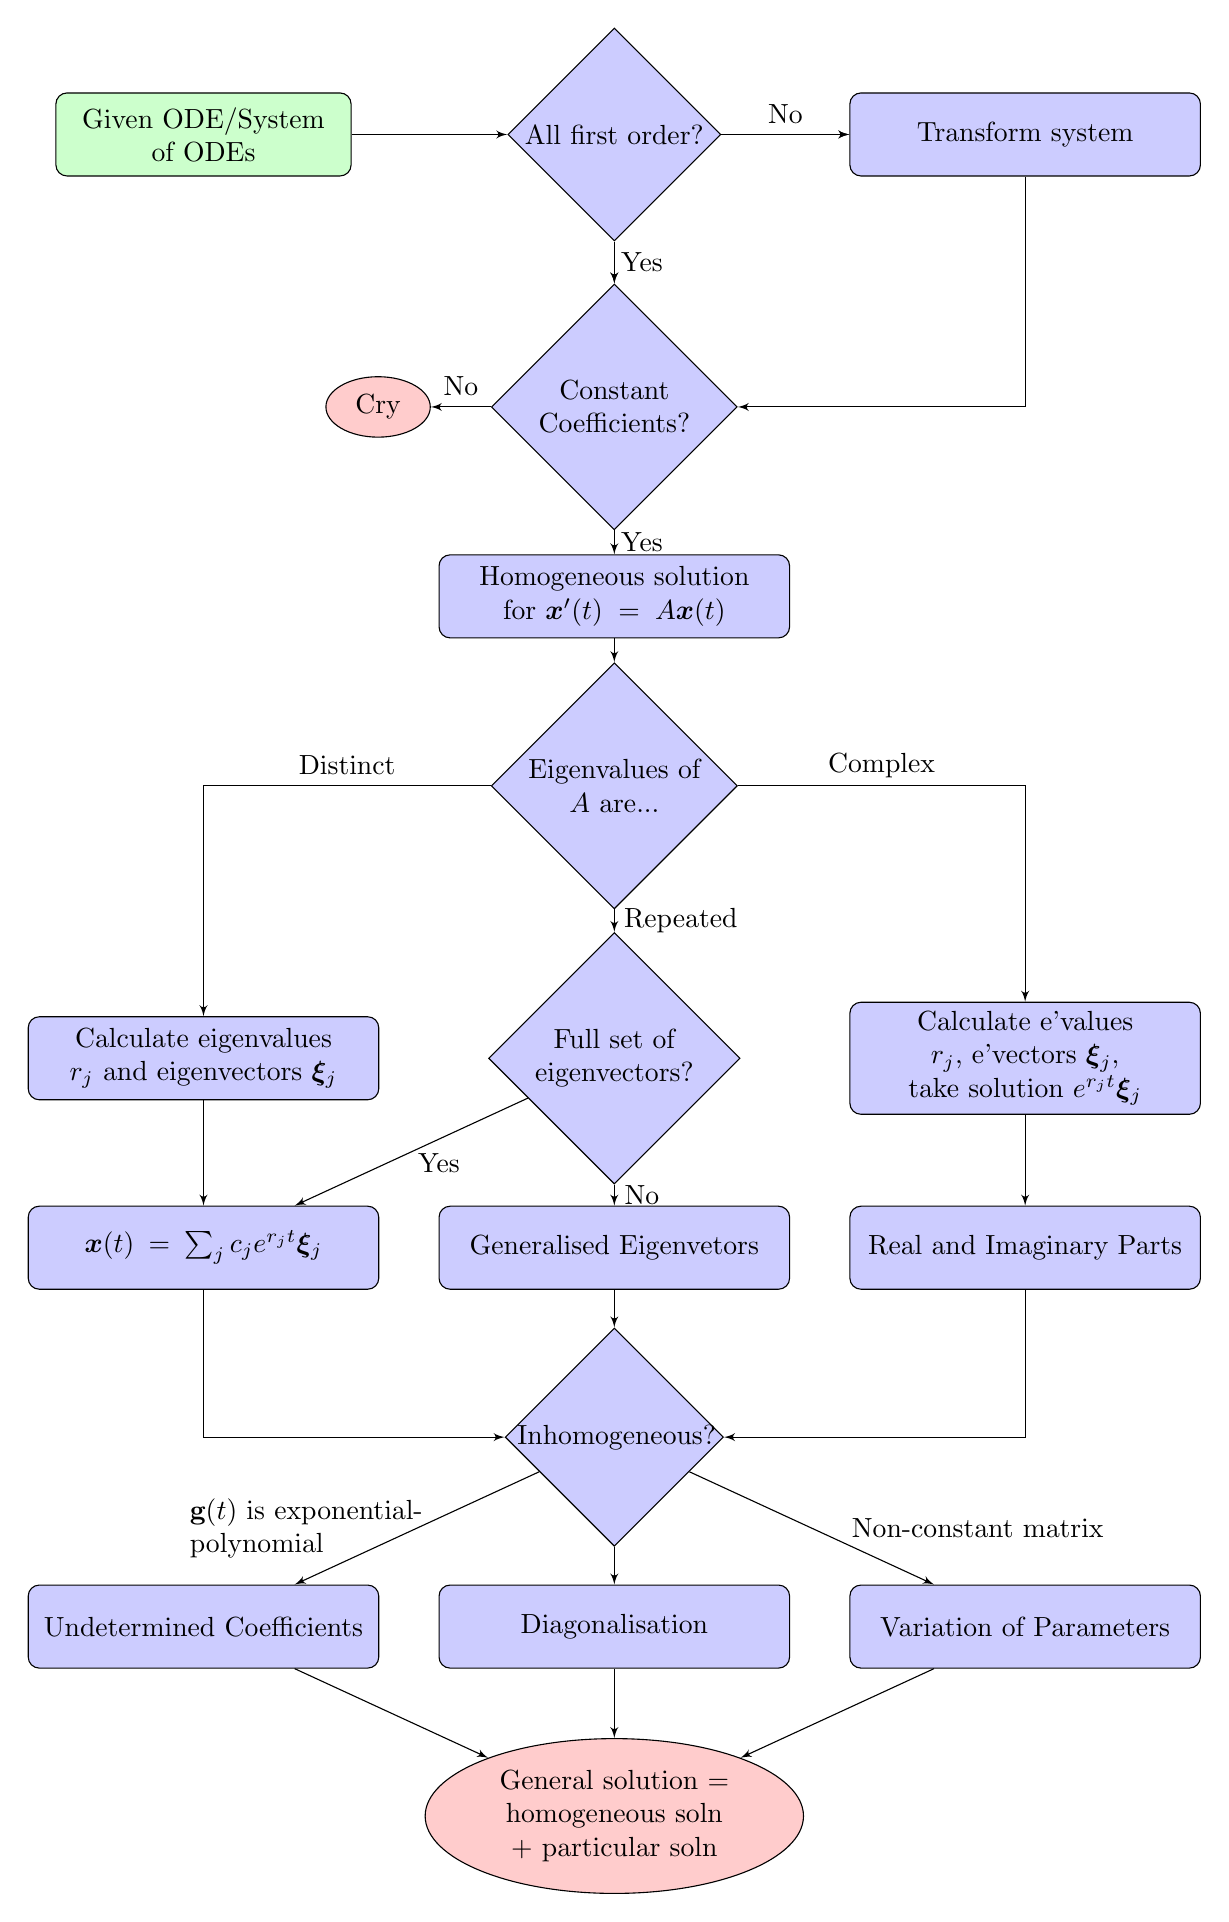
\begin{tikzpicture}
		% Place nodes
		\node [rectangle, draw, fill=green!20, text width=10em, text centered, rounded corners, minimum height=3em] (init) {Given ODE/System of ODEs};
		\node [decision, right of=init, xshift=12em] (allfo) {All first order?};
		\node [block, right of=allfo, xshift=12em] (transform) {Transform system};
		\node [decision, below of=allfo, yshift=-7em] (constcoeff) {Constant Coefficients?};
		\node [draw, ellipse,fill=red!20, node distance=3cm, minimum height=2em, text width=2em, text centered, left of=constcoeff] (cry) {Cry};
		\node [block, below of=constcoeff, yshift=-4em] (xtp) {Homogeneous solution for $\xtp = A\xt$};
		
		\node [decision, below of=xtp, yshift=-4em] (eigs) {Eigenvalues of $A$ are...};
		\node [decision, below of = eigs, yshift=-7em] (eigsrep) {Full set of eigenvectors?};
		\node [block, left of = eigsrep, xshift=-12em] (eigsdiscalc) {Calculate eigenvalues $r_j$ and eigenvectors $\xib_j$};
		\node [block, below of = eigsrep, yshift=-4em] (geneigs) {Generalised Eigenvetors};
		\node [block, left of=geneigs, xshift=-12em] (eigsdissol) {$\xt = \sum_j c_je^{r_jt}\xib_j$};
		\node [block, right of = eigsrep, xshift=12em] (eigscomcalc) {Calculate e'values $r_j$, e'vectors $\xib_j$, take solution $e^{r_jt}\xib_j$};
		\node [block, right of=geneigs, xshift=12em] (eigscomsol) {Real and Imaginary Parts};
		
		\node [decision, below of = geneigs, yshift=-4em] (inhomo) {Inhomogeneous?};
		\node [block, below of = inhomo, yshift=-4em] (diag) {Diagonalisation};
		\node [block, left of = diag, xshift=-12em] (undetcoeff) {Undetermined Coefficients};
		\node [block, right of = diag, xshift=12em] (varparam) {Variation of Parameters};
		\node [cloud, below of = diag, yshift=-4em] (gensol) {General solution = homogeneous soln + particular soln};
		
		% Draw edges
		\path [line] (init) -- (allfo);
		\path [line] (allfo) -- (transform);
		\path [line] (allfo) -- (constcoeff);
		\path [line] (allfo) -- node [yshift=0.74em] {No} (transform);
		\path [line] (allfo) -- node [xshift=1em] {Yes} (constcoeff);
		
		\path [line] (transform) |- (constcoeff);
		\path [line] (constcoeff) -- node [yshift=0.74em] {No} (cry);
		\path [line] (constcoeff) -- node [xshift=1em] {Yes} (xtp);
		
		\path [line] (xtp) -- (eigs);
		\path [line] (eigs) -| node [near start, yshift=0.74em] {Distinct} (eigsdiscalc);
		\path [line] (eigsdiscalc) -- (eigsdissol);
		\path [line] (eigs) -- node [xshift=2.4em] {Repeated} (eigsrep);
		\path [line] (eigs) -| node [near start, yshift=0.74em] {Complex} (eigscomcalc);
		\path [line] (eigscomcalc) -- (eigscomsol);
		\path [line] (eigsrep) -- node [yshift=-0.4em, xshift=1em] {Yes} (eigsdissol);
		\path [line] (eigsrep) -- node [xshift=1em] {No} (geneigs);
		
		\path [line] (eigsdissol) |- (inhomo);
		\path [line] (geneigs) -- (inhomo);
		\path [line] (eigscomsol) |- (inhomo);
		
		\path [line] (inhomo) -- node [align=left, xshift=-4em] {$\gt$ is exponential-\\polynomial} (undetcoeff);
		\path [line] (inhomo) -- node [align=left, xshift=6em] {Non-constant matrix} (varparam);
		\path [line] (inhomo) -- (diag);
		\path [line] (undetcoeff) -- (gensol);
		\path [line] (diag) -- (gensol);
		\path [line] (varparam) -- (gensol);
	\end{tikzpicture}
\end{center}
\end{small}

\section{Numerical Methods}

In this section, we aim to find a numerical approximation $\{x_n\}$ to $x(t)$ at discrete times $t_n$.

In general, we take a differential equation of the form
\[
x' = f(x, t),
\]
and times $t_n$ are given by
\[
t_n = t_0 + nh,
\]
where $h$ is the time step.

\subsection{Euler's Method}

The Euler Method involves approximating $x_{n+1}$ using the tangent line (see \Cref{fig:euler}). To see this, observe that
\[
\frac{x(t_{n+1}) - x(t_n)}{t_{n+1} - t_n} = \frac{x(t_{n+1}) - x(t_n)}{h} \approx f(x(t_n), t_n).
\]
Replacing the exact values $x(t_n)$ with $x_n$ and rearranging, we find the following iterative formula that is Euler's Method:
\begin{equation}\label{eq:euler}
	x_{n+1} = x_n + h f(x_n, t_n).
\end{equation}

\begin{figure}[!ht]
	\centering
	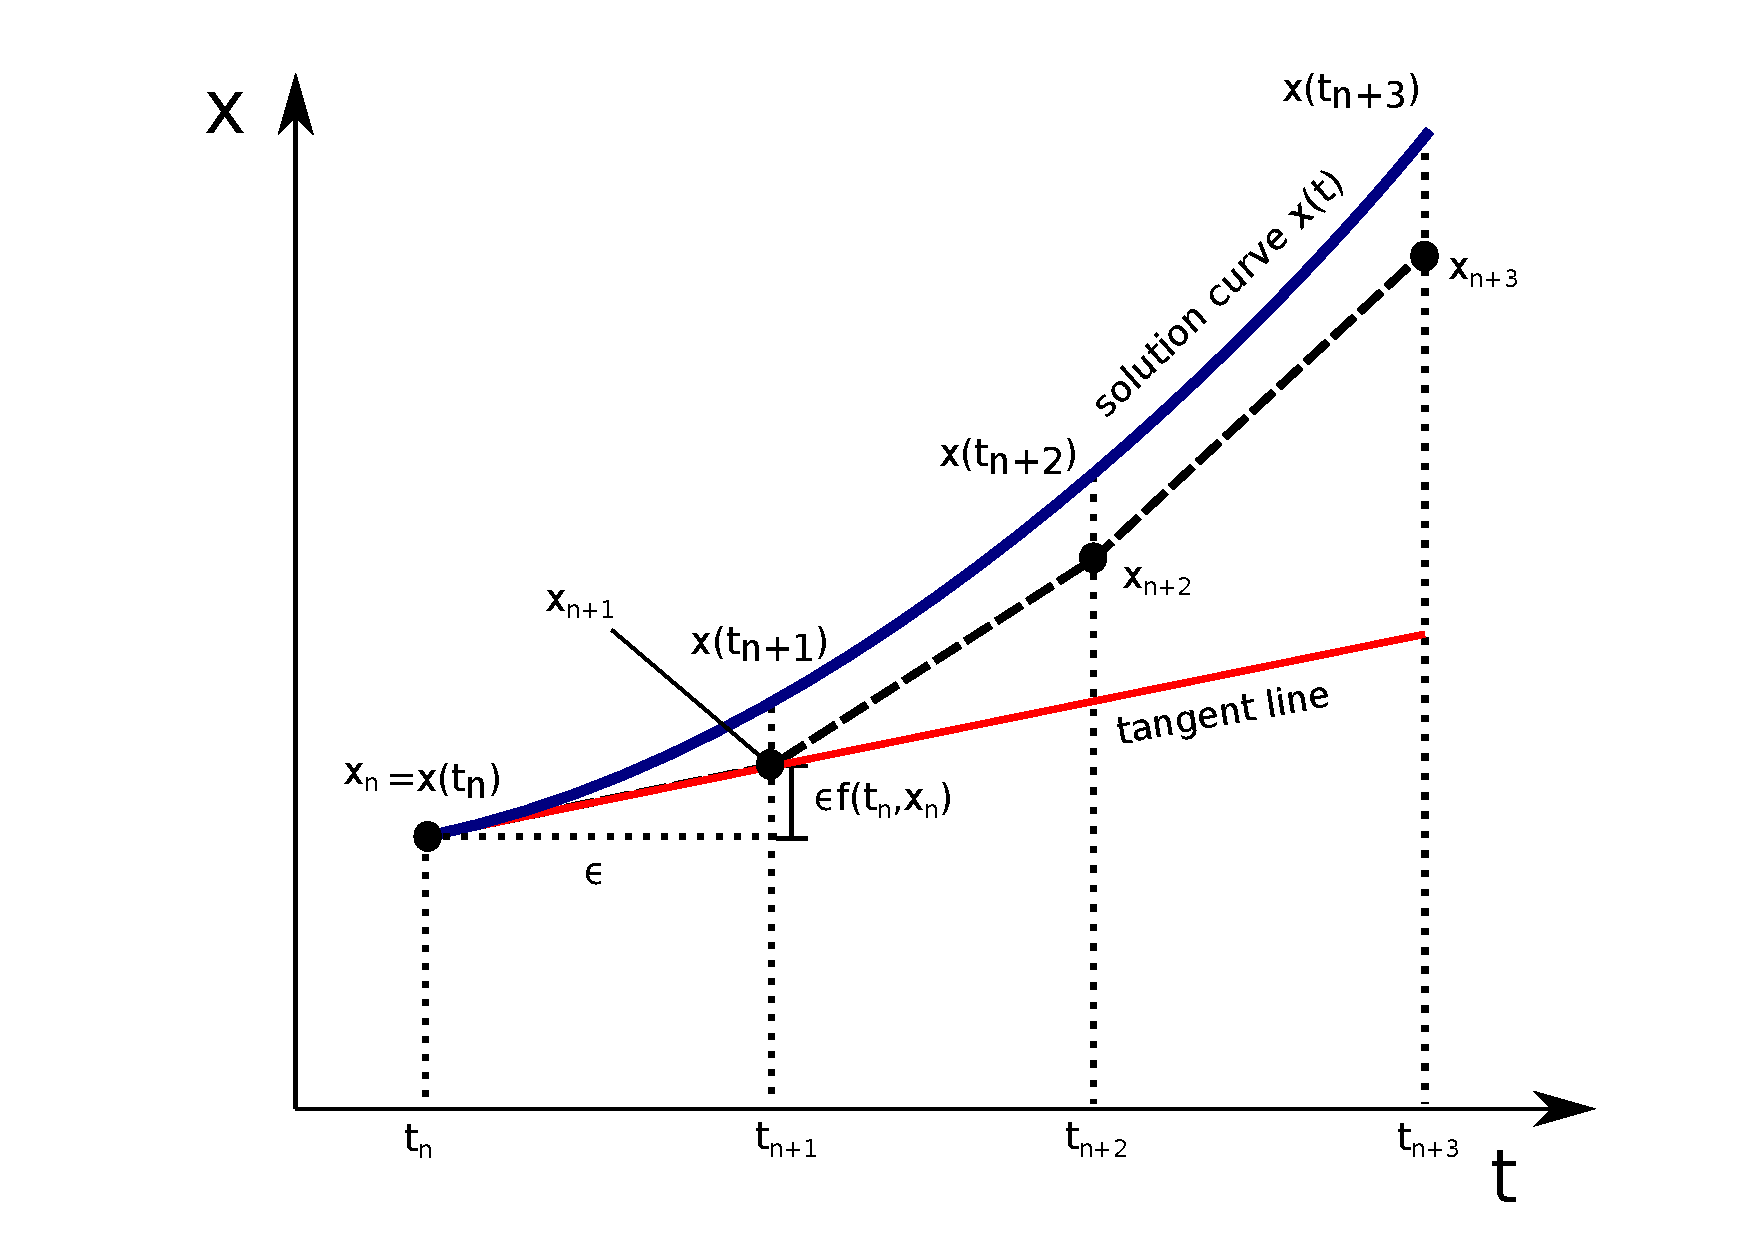
\includegraphics[width=0.65\textwidth]{euler.pdf}
	\caption{Illustration of multiple iterations of Euler's method. Note that $\epsilon$ in this diagram is equivalent to our time step $h$. \cite[Figure 2]{numgraph}.}
	\label{fig:euler}
\end{figure}

There are a couple of general ways of deriving numerical approximations:
\begin{enumerate}
	\item{\textbf{Integral Equation:} \[x(t_{n+1}) = x(t_n) + \int_{t_n}^{t_{n+1}} f(x(s), s) \,ds.\] Then different approximations arise by considering ways that $\int_{t_n}^{t_{n+1}} f(x(s), s) \,ds$ may be approximated though the area under the curve.}
	\item{\textbf{Taylor Expansion:} \[x(t_{n+1}) = x(t_n + h) = x(t_n) + hx'(t_n) + \frac{h^2}{2}x''(t_n) + \cdots\] From this, approximations may be made by, for example, taking the first $k$ terms of the expansion. Another useful form of Taylor's theorem is the following: \[x(t_n + h) = x(t_n) + hx'(t_n) + \frac{h^2}{2}x''(\overline{t}_n)\] for some $\overline{t}_n$ between $t_n$ and $t_{n+1}=t_n+h$.}
\end{enumerate}

\begin{exercise}
	Derive \Cref{eq:euler} using both the method of integral equations (see \Cref{fig:eulerint}) and using the Taylor expansion.
\end{exercise}

\begin{figure}[!ht]
	\centering
	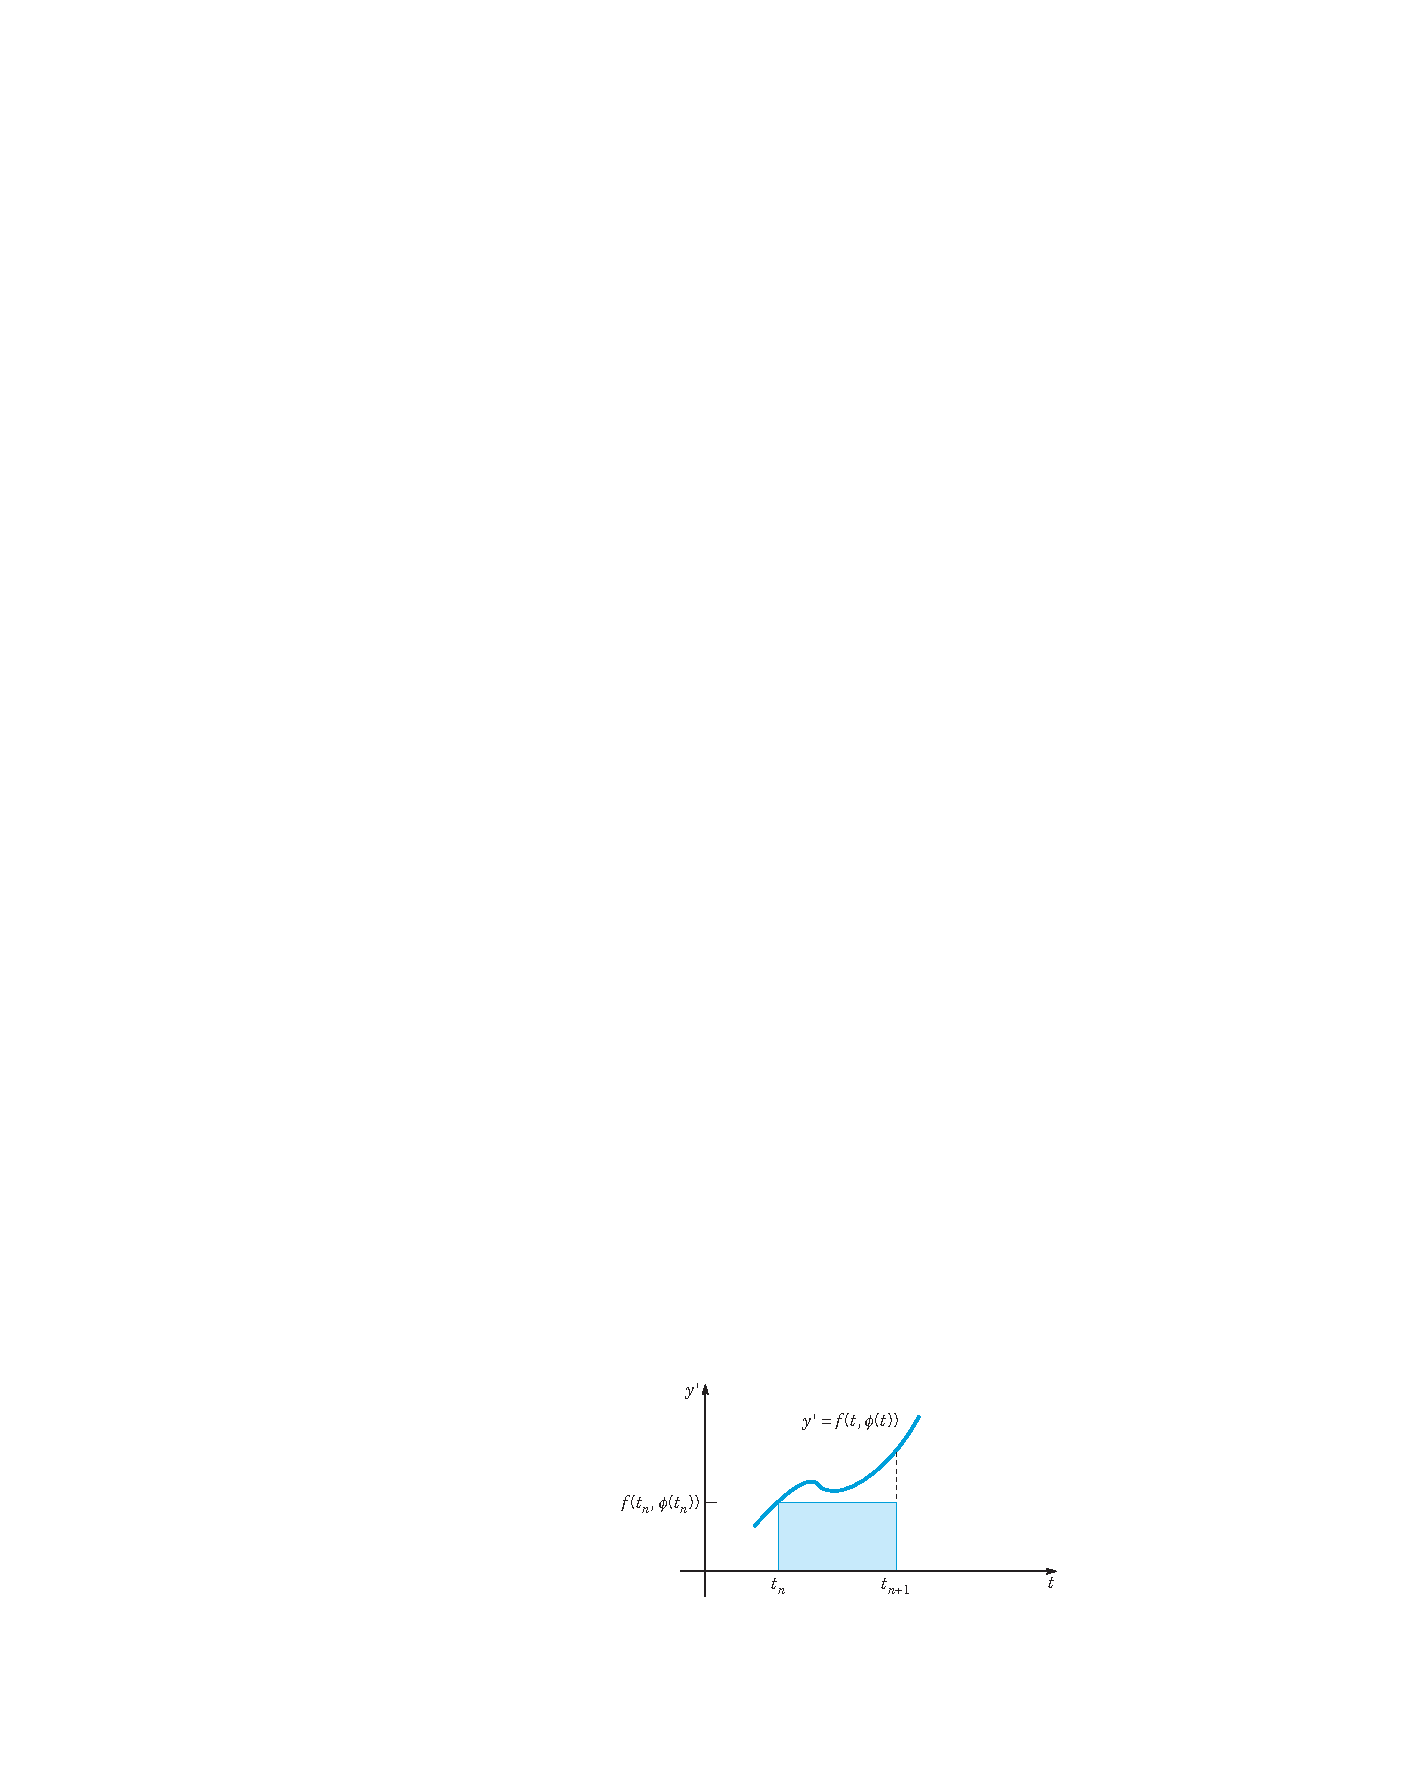
\includegraphics[width=0.6\textwidth]{integralEquationEuler.pdf}
	\caption{Derivation of the Euler method using the integral equation \cite[Figure 8.1.1]{boyce}.}
	\label{fig:eulerint}
\end{figure}

The formula in \Cref{eq:euler} is also called the Forward Euler Method, and its cousin is the Backward Euler Method. We can derive this method using the integral equation and approximating the integral by a rectangle with width $h$ and height $f(x_{n+1}, t_{n+1})$:
\begin{equation}
	x_{n+1} = x_n + h f(x_{n+1}, t_{n+1}).
\end{equation}

Note that this is an implicit method (requiring extra work to solve for $x_{n+1}$) compared to the Forward Euler which is explicit.

Once we are comfortable with representing the differential equation as an integral equation and approximating areas, we can find many more schemes for numerical approximations, for example the Trapezoidal rule:
\begin{equation}
	x_{n+1} = x_n + h \frac{f(x_n, t_n)+f(x_{n+1}, t_{n+1})}{2},
\end{equation}
and the Implicit Midpoint rule:
\begin{equation}
	x_{n+1} = x_n + h f\left(\frac{x_n+x_{n+1}}{2}, \frac{t_n+t_{n+1}}{2}\right).
\end{equation}

\begin{remark}
	All of these methods can be easily applied to systems of ODEs of the form $\vbx' = \bm{f}(\vbx, t)$ by replacing the scalar $x_n$, $f(x,t)$, etc. with vector quantities: $\vbx_n$, $\bm{f}(\vbx, t)$, etc.
\end{remark}

\begin{eg}
	Consider the ODE $y' = 2y - 3t$ with initial condition $y(0)=1$. Use the forward Euler method with $h=0.1$ to obtain an approximation for the solution to the IVP at $t=0.4$.
	
	The initial condition becomes the first point, $y_0 = 1$. Then applying the Euler method:
	\begin{align*}
		y_1 &= y_0 + hf(x_0, t_0) = 1 + 0.1 (2\cdot 1 - 3\cdot 0) = 1.2 \\
		y_2 &= y_1 + hf(x_1, t_1) = 1.2 + 0.1 (2\cdot 1.2 - 3\cdot 0.1) = 1.41 \\
		y_3 &= y_2 + hf(x_2, t_2) = 1.41 + 0.1 (2\cdot 1.41 - 3\cdot 0.2) = 1.632 \\
		y_4 &= y_3 + hf(x_3, t_3) = 1.632 + 0.1 (2\cdot 1.632 - 3\cdot 0.3) = 1.8684
	\end{align*}
	So $y(0.4) \approx 1.8684$.
\end{eg}


\subsection{Errors}

In a numerical approximation, there are three sources of errors:
\begin{enumerate}
	\item Approximation of $x' = f(x,t)$ between $x_n$ and $x_{n+1}$.
	\item Error in $x_n$ (because of errors incurred in previous steps).
	\item Round off errors.
\end{enumerate}

We will consider three types of errors:
\begin{enumerate}
	\item Global truncation error: $E_n = x(t_n) - x_n$.
	\item Round off error: $R_n = x_n - X_n$, where $X_n$ is the result with round-off.
	\item Local error $e_n = x(t_n) - x_n^*$, where $x_n^*$ is the error incurred after one time step by assuming we start on the true curve, i.e. $x_{n-1}^* = x(t_{n-1})$.
\end{enumerate}

In practice, it may be required to take the absolute value of $E_n$, $R_n$, and $e_n$ since we want the error measurement to be positive.

\begin{eg}
	We will calculate the local and global errors in the Forward Euler Method. Beginning with the Taylor expansion:
	\begin{align*}
		x(t_n) &= x(t_{n-1} + h) \\ 
		&= x(t_{n-1}) + hx'(t_{n-1}) + \frac{h^2}{2}x''(\overline{t}_n) \tag{$t_{n-1} \leq \overline{t}_n \leq t_n$} \\
		&= x^* + hf(x^*, t_{n-1}) + \frac{h^2}{2}x''(\overline{t}_n).
	\end{align*}
	In addition,
	\[
	x_n = x^* + h f(x^*, t_{n-1}),
	\]
	therefore
	\[
	x(t_n) - x_n = e_n = \frac{h^2}{2}x''(\overline{t}_n).
	\]
	If $x''(t)$ is bounded, then we can write
	\[
	|e_n| \leq M h^2 \implies e_n = O(h^2).
	\]
	Now to find the global error by supposing that we make the local error $n$ times:
	\begin{align*}
		E_n &= x(t_n) - x_n, \quad n = \frac{t_n-t_0}{h} \\
		|E_n| &\leq M h^2 n = M h^2 \frac{t_n-t_0}{h} = Kh \\
		\implies E_n &= O(h).
	\end{align*}
	Therefore we say that the Forward Euler Method is a first-order method (or that it is first-order accurate).
\end{eg}

\begin{remark}
	Generally, a method is of order $p$ if $|E_n| \leq K h^p$ i.e. $E_n = O(h^p)$.
\end{remark}

\subsection{Heun Method}

To derive the Heun Method, we begin with the integral equation
\begin{align*}
	x(t_{n+1}) &= x(t_n) + \int_{t_n}^{t_{n+1}} f(x(s), s) \,ds \\
	&\approx x(t_n) + \frac{h}{2} (f(x(t_n), t_n) + f(x(t_{n+1}), t_{n+1})),
\end{align*}
using a trapezoidal approximation of the integral (see \Cref{fig:heunint}).

Now, we can use the approximation
\[
x(t_{n+1}) \approx x(t_n) + h f(x(t_n), t_n)
\]
(i.e. the Forward Euler Method) to write
\begin{equation}
	x_{n+1} = x_n + \frac{h}{2}\left[f(x_n,t_n) + f(x_n + hf(x_n,t_n), t_{n+1})\right].
\end{equation}
This is the Heun Method (or Heun's Method).

\begin{figure}[!ht]
	\centering
	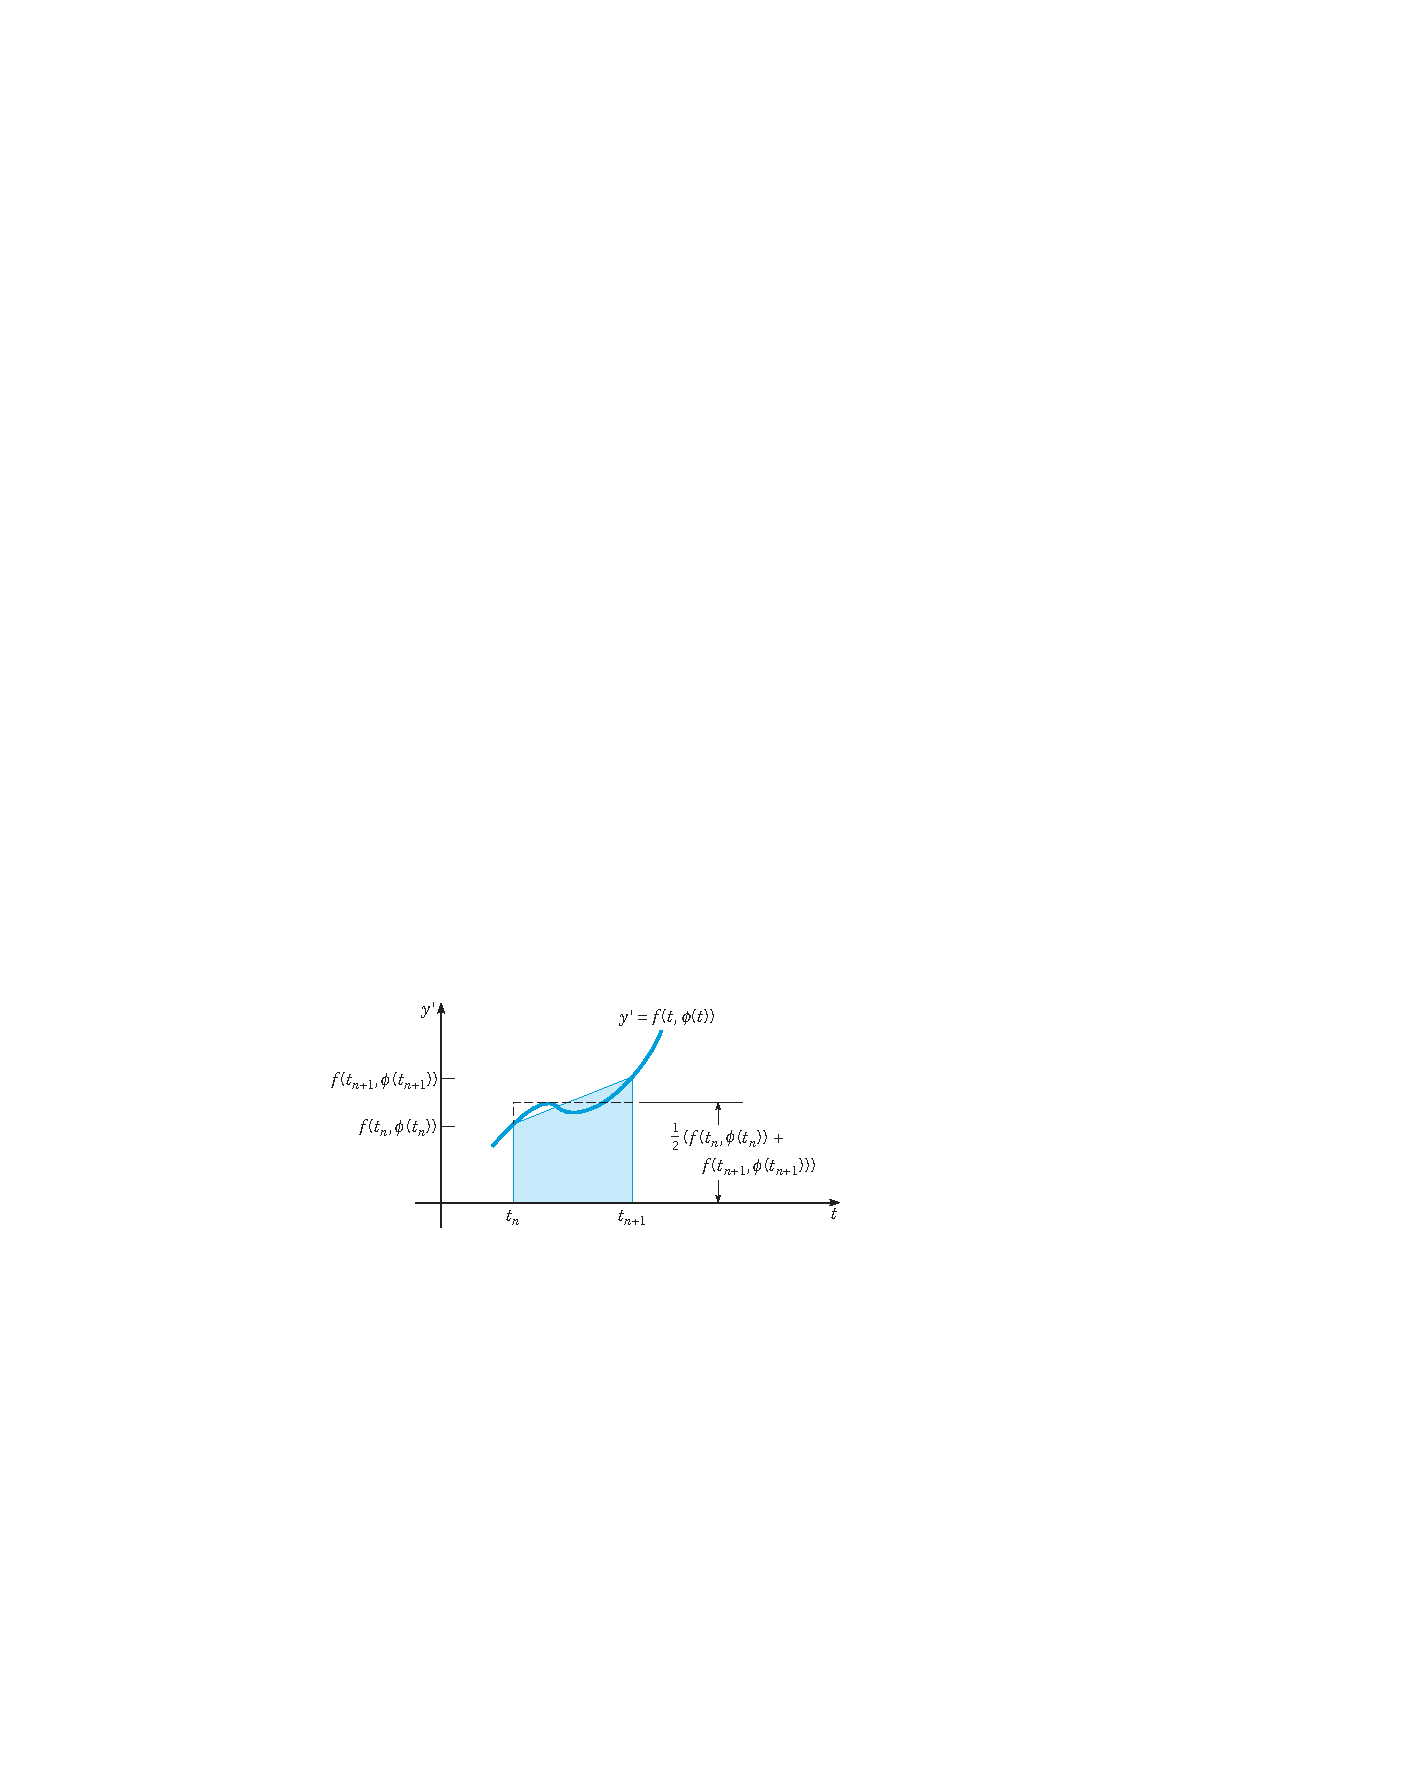
\includegraphics[width=0.6\textwidth]{integralEquationHeun.pdf}
	\caption{Derivation of the Heun method using the integral equation \cite[Figure 8.2.1]{boyce}.}
	\label{fig:heunint}
\end{figure}

\begin{remark}
	It can be shown that the local error of this method if $O(h^3)$ and the global error is $O(h^2)$, this the order of Heun's Method is 2.
\end{remark}

Heun's Method is an example of a multistage method. Compared to a single-step method like Euler's Method where only one point and its derivative was used to determine the next value, a multistage method takes some intermediate steps and then refers to multiple previous points in the final calculation. To see this explicitly, we can express Heun's Method as follows, with two explicit 'steps' $k_1$ and $k_2$:
\begin{align*}
	k_1 &= f(x_n, t_n) \\
	k_2 &= f(x_n + hk_1, t_n+h) \\
	x_{n+1} &= x_n + \frac{h}{2}(k_1 + k_2).
\end{align*}

\subsection{Runge-Kutta Methods}

A family of multistep methods is the group of Runge-Kutta methods. The most widely known member of this family is the four-step version (also known as RK4), which may be illustrated as follows:
\begin{align*}
	k_1 &= f(x_n, t_n) \\
	k_2 &= f(x_n + \frac{hk_1}{2}, t_n + \frac{h}{2}) \\
	k_3 &= f(x_n + \frac{hk_2}{2}, t_n + \frac{h}{2}) \\
	k_4 &= f(x_n + hk_3, t_n + h) \\
	x_{n+1} &= x_n + \frac{h}{6} (k_1 + 2k_2 + 2k_3 + k_4).
\end{align*}

This is a fourth order method, i.e. $E_n = O(h^4)$ and $e_n = O(h^5)$.

\subsection{Adams-Bashforth Method}

This family of methods uses $x_n, x_{n-1}, \dots$ to compute $x_n$. We take the case of using only $x_n$ and $x_{n-1}$. 

Reminding ourselves of the integral equation,
\[
x(t_{n+1}) = x(t_n) + \int_{t_n}^{t_{n+1}} f(x(s), s) \,ds,
\]
we approximate $f$ by $f(s) = as + b$.\footnote{Note that this illustration is for an autonomous system, i.e. one where $f$ does not depend on $t$, but an analogous form of the method exists for non-autonomous systems.}

We then must find $a$ and $b$ such that 
\begin{align*}
	f(x_{n-1}) &= a t_{n-1}+b \\
	f(x_n) &= a t_n + b.
\end{align*}

Solving for $a$ and $b$, we obtain
\[
a = \frac{f(x_n)-f(x_{n-1})}{h} \quad \text{and} \quad b = \frac{f(x_{n-1})t_n - f(x_n)t_{n-1}}{h}.
\]

Returning to the integral equation,
\[
x_{n+1} = x_n + \int_{t_n}^{t_{n+1}} as + b \,ds = a \frac{t_{n+1}^2 - t_n^2}{2} + b(t_{n+1} - t_n).
\]

To simplify, we first write $t_{n+1}^2 - t_n^2 = (t_{n+1} - t_n)(t_{n+1}+t_n) = h (t_{n+1}+t_n)$ for constant step size $h = t_{n+1} - t_n$. Then
\begin{align*}
	\frac{a}{2}(t_{n+1}^2 - t_n^2) + b(t_{n+1} - t_n) &= \frac{f_n - f_{n-1}}{2}(t_{n+1}+t_n) + f_{n-1}t_n - f_n t_{n-1} \\ 
	&= \frac12(f_n t_{n+1} + f_nt_n - f_{n-1}t_{n+1} - f_{n-1}t_n) + f_{n-1}t_n - f_n t_{n-1} \\ 
	&= f_n(\frac12 t_{n+1} + \frac12 t_n - t_{n-1}) + \frac12 f_{n-1}(t_n - t_{n+1}).
\end{align*}

Then $t_n - t_{n+1} = -h$ clearly, and $\frac12 t_{n+1} + \frac12 t_n - t_{n-1} = \frac12 t_n + \frac12 h + \frac12 t_n - t_{n-1} = \frac32 h$, hence we get the following simplified formula:
\begin{equation}
	x_{n+1} = x_n + \frac{h}{2}\left(3f(x_n) - f(x_{n-1})\right).
\end{equation}

\vfill
\pagebreak
\subsection{Comparison of Methods in Practice}

A comparison of the four methods discussed in this section is shown in \Cref{fig:numericals}. The particular example is the harmonic oscillator, where
\begin{align*}
	x' &= y \\
	y' &= -x.
\end{align*}

\begin{figure}[!ht]
	\centering
	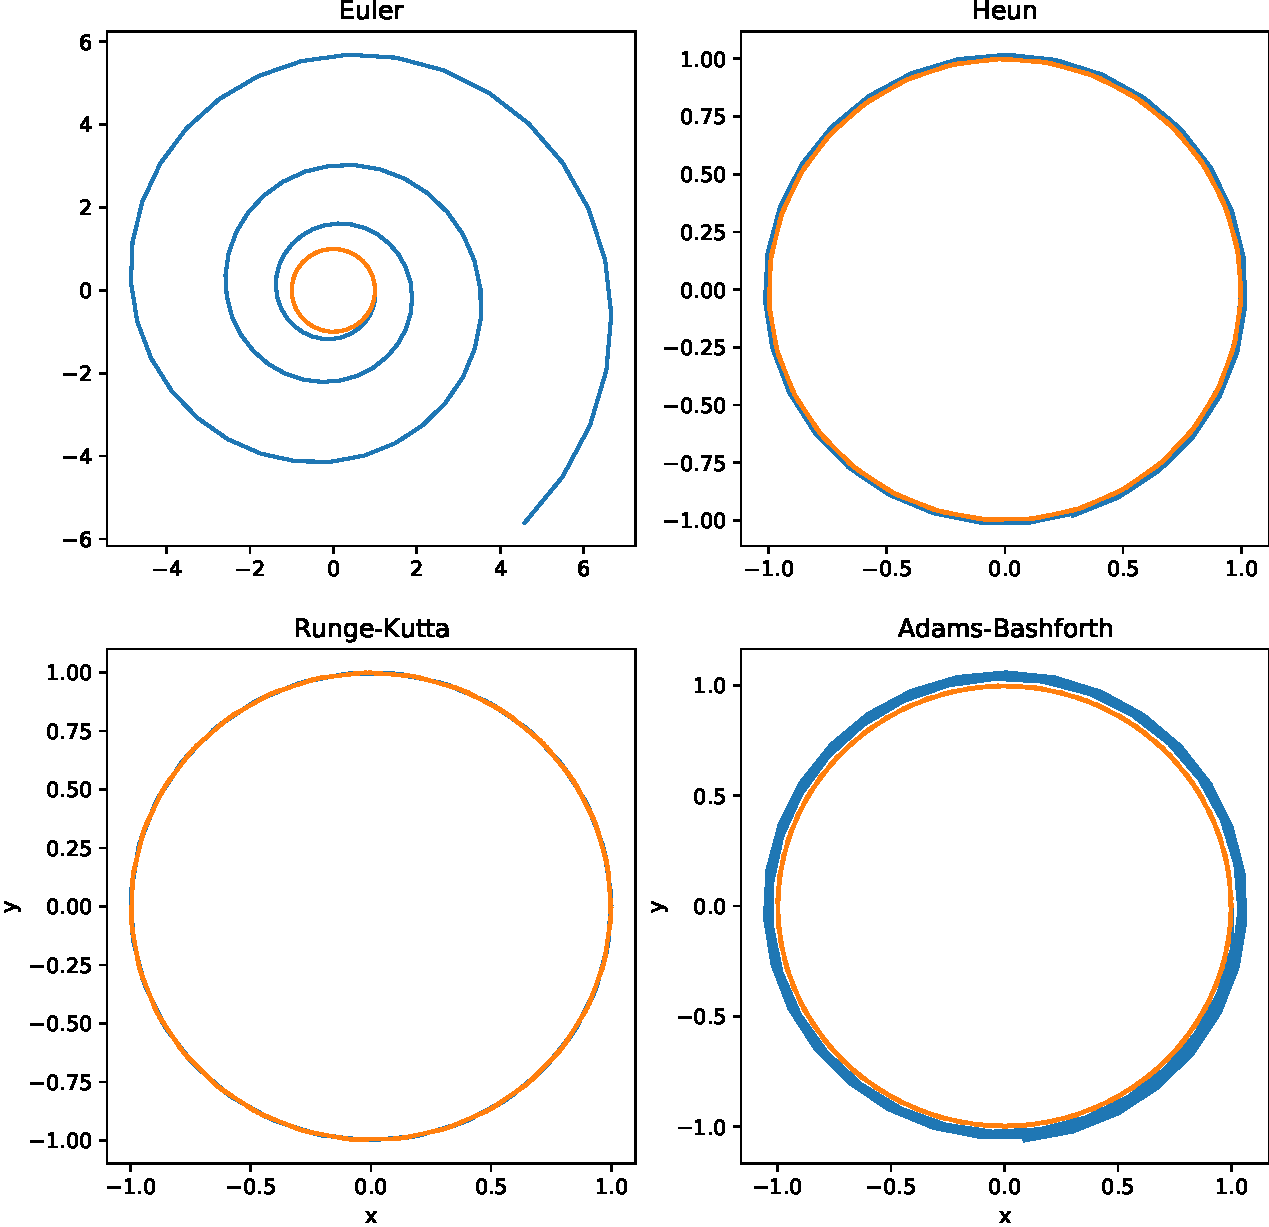
\includegraphics[width=0.9\textwidth]{NumericalMethods.pdf}
	\caption{Comparison of the results of the Euler, Heun, Runge-Kutta, and Adams-Bashforth methods (blue) in approximating an ODE. The true solution is shown in orange.}
	\label{fig:numericals}
\end{figure}
\section{Non-linear Systems of ODEs}

Since many differential equations cannot be solved conveniently by analytical methods, it is important to consider what qualitative information can be obtained about their solutions without actually solving the equations. Studying the qualitative theory tells us the general behaviour of the ODE for all possible trajectories. There are two aspects to this theory:
\begin{itemize}
	\item Looking at the ODE locally near $\xta$,
	\item Global aspect across $\R^n$.
\end{itemize}

We will now focus on $\vbx = (x, y) \in \R^2$ where 
\begin{equation}\label{eq:linearsystem2}
	\begin{cases}
		x' = F(x,y) \\
		y' = G(x,y)
	\end{cases}
\end{equation}
Since $F$ and $G$ can be arbitrary, the problem is generally non-linear.

The terminology used here might be useful in the content that follows: the $(x,y)$ plane is a \vb{phase plane}, where vector fields are plotted and a representative set of trajectories is referred to as a \vb{phase portrait}.

\begin{definition}
	A point $\vbx_0 = (x_0, y_0)$ is a \textbf{critical point} if $F(x_0, y_0) = G(x_0, y_0) = 0$.
\end{definition}

\begin{theorem}[Rectification theorem]
	Consider $\xta = (x_{\ast}, y_{\ast})$ such that $(F(\xta), G(\xta)) \neq (0,0)$. Then, in a neighbourhood of $\xta$, there is a smooth change of variables $(x,y) \mapsto (\Tilde{x}, \Tilde{y})$ that transforms the ODE into 
	\[
	\begin{cases}
		\Tilde{x}' = 1 \\
		\Tilde{y}' = 0
	\end{cases}
	\]
\end{theorem}

If $(F(\xta), G(\xta)) = (0,0)$, then $\xta$ is a \vb{critical point}, also known as an equilibrium point or a fixed point. If $\vbx(0) = \xta$, then $\xt = \xta$ for all $t$, since both $x'$ and $y'$ are zero so $x$ and $y$ will not change over time when we start at a critical point.

\subsection{Linear Approximation near a Critical Point}\label{sec:linearapproxcp}

Let $\xta = (x_{\ast},y_{\ast})$ be a critical point. Then $F(\xta) = G(\xta) = 0$. We have the following system of equations:
\[
\begin{cases}
	x(t) = x_{\ast} + u(t) \\
	y(t) = y_{\ast} + v(t)
\end{cases}
\]
where $u(t), v(t)$ are perturbations of $x$ and $y$ respectively.

The system in \Cref{eq:linearsystem2} is locally in the neighbourhood of $\xta$ whenever the functions $F$ and $G$ have continuous partial derivatives up to order two. To show this, we use Taylor expansions about the point $\xta$ to write $F(x, y)$ and $G(x, y)$ in the form:
\[ 
u' = F(x_{\ast} + u, y_{\ast} + v) = F(\xta) + \p_x F(\xta)u + \p_y F(\xta)v + \eta_1 \xt \]
\[
v' = G(x_{\ast} + u, y_{\ast} + v) = G(\xta) + \p_x G(\xta)u + \p_y G(\xta)v + \eta_2 \xt
\]

We can now notice that
\[
\frac{\eta_i}{\Vert \vbx - \xta \Vert} \rightarrow 0 \text{ as } \vbx \rightarrow \xta,
\]
and since $F(\xta) = G(\xta)=0$, we now have a linear system of ODEs of the form
\begin{equation}\label{3.2}
	\mat{u'\\v'} = \mat{\p_x F(\xta) & \p_y F(\xta) \\ \p_x G(\xta) & \p_y G(\xta)} \mat{u\\v},
\end{equation}
where $J = \mat{\p_x F(\xta) & \p_y F(\xta) \\ \p_x G(\xta) & \p_y G(\xta)}$ is called the \vb{Jacobian matrix}.

Since the Jacobian is calculated at the Critical point $\xta$, it is a constant matrix that gives a linear system that can be solved using methods from \Cref{sec:firstorder}.

\begin{eg}[Damped Pendulum]\label{eg:dampedpendulum} Consider the equations:
	\begin{align*}
		x' &= y = F(\xta)\\
		y' &= -\omega^2 \sin{x} - \gamma y = G(\xta)
	\end{align*}
	(For the physicists out there, $\omega = \sqrt{\frac{g}{L}}$, where $g$ is the gravitational constant, $L$ is the length of the pendulum, and $\gamma$ is the friction coefficient)
	
	We find the critical points ($x'=y'=0$) to be:
	\[
	y=0 
	\]
	\[
	-\omega^2 \sin{x} - \gamma y = 0 \implies -\omega^2 \sin{x} = 0 \implies\sin{x} = 0 \implies x = n\pi
	\]
	where $n \in \Z$. We find the Jacobian to be given by:
	\[
	J(x,y) = \mat{
		\p_x F(\xta) & \p_y F(\xta) \\ \p_x G(\xta) & \p_y G(\xta)} = \mat{ 0 & 1 \\ 
		-\omega^2 \cos{x} & -\gamma}
	\]
	At the critical points, 
	\[
	J(n\pi,0) = \mat{ 0 & 1 \\ -\omega^2(-1)^n & -\gamma}
	\]
	which depends on the value of $n$ as $\cos{x} = -1$ for odd $n$ and $\cos{x} = 1$ for even $n$. The system is now given by 
	\[
	\mat{u'\\v'} = \mat{0 & 1 \\ -\omega^2(-1)^n & -\gamma} \mat{u\\v}
	\]
	which can be solved using \Cref{sec:firstorder} (left as an exercise for the reader).
	
	A vector field generated in Python in the style of \Cref{fig:geomsys} is shown in \Cref{fig:pendulumpython}.
\end{eg}

\begin{figure}[H]
	\centering
	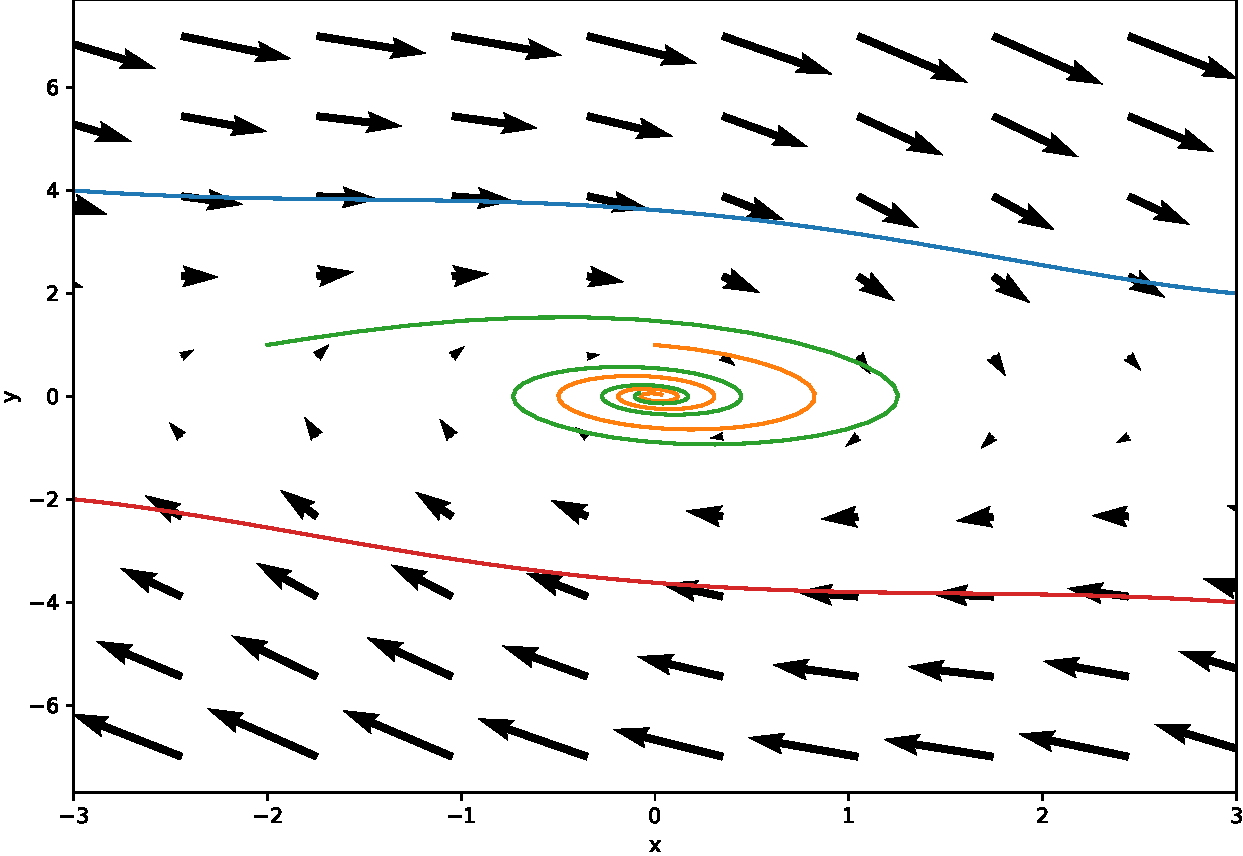
\includegraphics[width=0.7\textwidth]{vectorFieldPendulum.pdf}
	\caption{Direction field and selected solution trajectories for the damped pendulum.}
	\label{fig:pendulumpython}
\end{figure}

\subsection{Classification of Critical points}

We now consider 2-dimensional systems of the form: 
\[
\begin{cases}
	x' = F(x,y) \\
	y' = G(x,y) 
\end{cases}
\]

For the critical point $\xta = (x_{\ast}, y_{\ast})$, let $x(t) = x_{\ast} + u(t)$ and $y(t) = y_{\ast} + v(t)$. As seen above, we have a linearised system for $\mat{u'\\v'}$ as given in \Cref{3.2}. So upon solving, $\mat{u'\\v'}$ we have solutions of the form: 
\begin{equation}\label{3.5}
	\mat{u(t)\\v(t)} = 
	c_1 e^{r_1t} \xib_1 + c_2 e^{r_2t} \xib_2
\end{equation}
where $r_1, r_2$ are the eigenvalues of the Jacobian matrix $J(x,y)$ and $\xib_1, \xib_2$ are the associated eigenvectors.

Using these eigenvalues, we can predict the behaviour of the ODEs near critical points (see \Cref{table:stability} for a summary).
\begin{itemize}
	\item Case 1: Real Unequal Eigenvalues:
	\begin{enumerate}[label=(\roman*)]
		\item $r_1 < r_2 < 0$: \\
		Consider the solution $\xt = c_1 e^{r_1t} \xib_1 + c_2 e^{r_2t} \xib_2 = e^{r_2t} (c_1 e^{(r_1-r_2)t} \xib_1 + c_2 \xib_2)$. \\
		We now observe how $x$ changes as $t \to \pm \infty$: \\
		\underline{As $t \to \infty$}: if $c_2 \neq 0$, then the term $c_1 e^{(r_1-r_2)t} \xib_1$ is of negligible magnitude compared to $c_2 \xib_2$ for sufficiently large $t$, so $\xt \to 0$ along $\xib_2$.
		If $c_2 = 0$ (i.e. the solution starts on the line $\xib_1$) then $\xt \to 0$ along $\xib_1$. \\
		\underline{As $t \to -\infty$}: if $c_1 \neq 0$, then the dominant term is $c_1 e^{r_1t} \xib_1$ and $\xt \to \infty$ along $\xib_1$. 
		If $c_1 = 0$, then $|\xt| \to \infty$ along $\xib_2$. \\
		The critical point in this case is a \vb{nodal sink} (see \Cref{fig:trajectory1}).
		
		\item $r_1 > r_2 > 0$: \\
		Consider the solution $\xt = c_1 e^{r_1t} \xib_1 + c_2 e^{r_2t} \xib_2$. \\
		We now observe how $x$ changes as $t \to \pm \infty$: \\
		\underline{As $t \to \infty$}: if $c_1 \neq 0$, then $|\xt| \to \infty$ along $\xib_1$ as the $c_1 e^{r_1t} \xib_1$ term dominates.
		If $c_1 = 0$, then $|\xt| \to \infty$ along $\xib_2$. \\
		\underline{As $t \to -\infty$}: if $c_2 \neq 0$, then $\xt \to 0$ along $\xib_2$ as the $c_2 e^{r_2t} \xib_2$ term dominates.  
		If $c_2 = 0$, then $\xt \to 0$ along $\xib_1$. \\
		The critical point in this case is a \vb{nodal source} (essentially the same as \Cref{fig:trajectory1}, with the arrows all running in the opposite direction).
		
		\item $r_1 > 0 > r_2$: \\
		Consider the solution $\xt = c_1 e^{r_1t} \xib_1 + c_2 e^{r_2t} \xib_2$. \\
		We now observe how $x$ changes as $t \to \pm \infty$: \\
		As $t \to \infty$, the $c_1 e^{r_1t}\xib_1$ term dominates and $|\xt| \to \infty$. As $t \to -\infty$, the $c_2 e^{r_2t}\xib_2$ term dominates and $|\xt| \to \infty$ also. \\
		The exceptions are: \\
		$c_1 = 0$, in which case $x \to0$ as $t \to \infty$ since $r_2$ is negative. \\
		$c_2 = 0$, in which case $x \to0$ as $t \to -\infty$. \\
		The critical point in this case is a \vb{saddle point} (see \Cref{fig:trajectory2}).
	\end{enumerate}
	
	\begin{figure}[H]
		\centering
		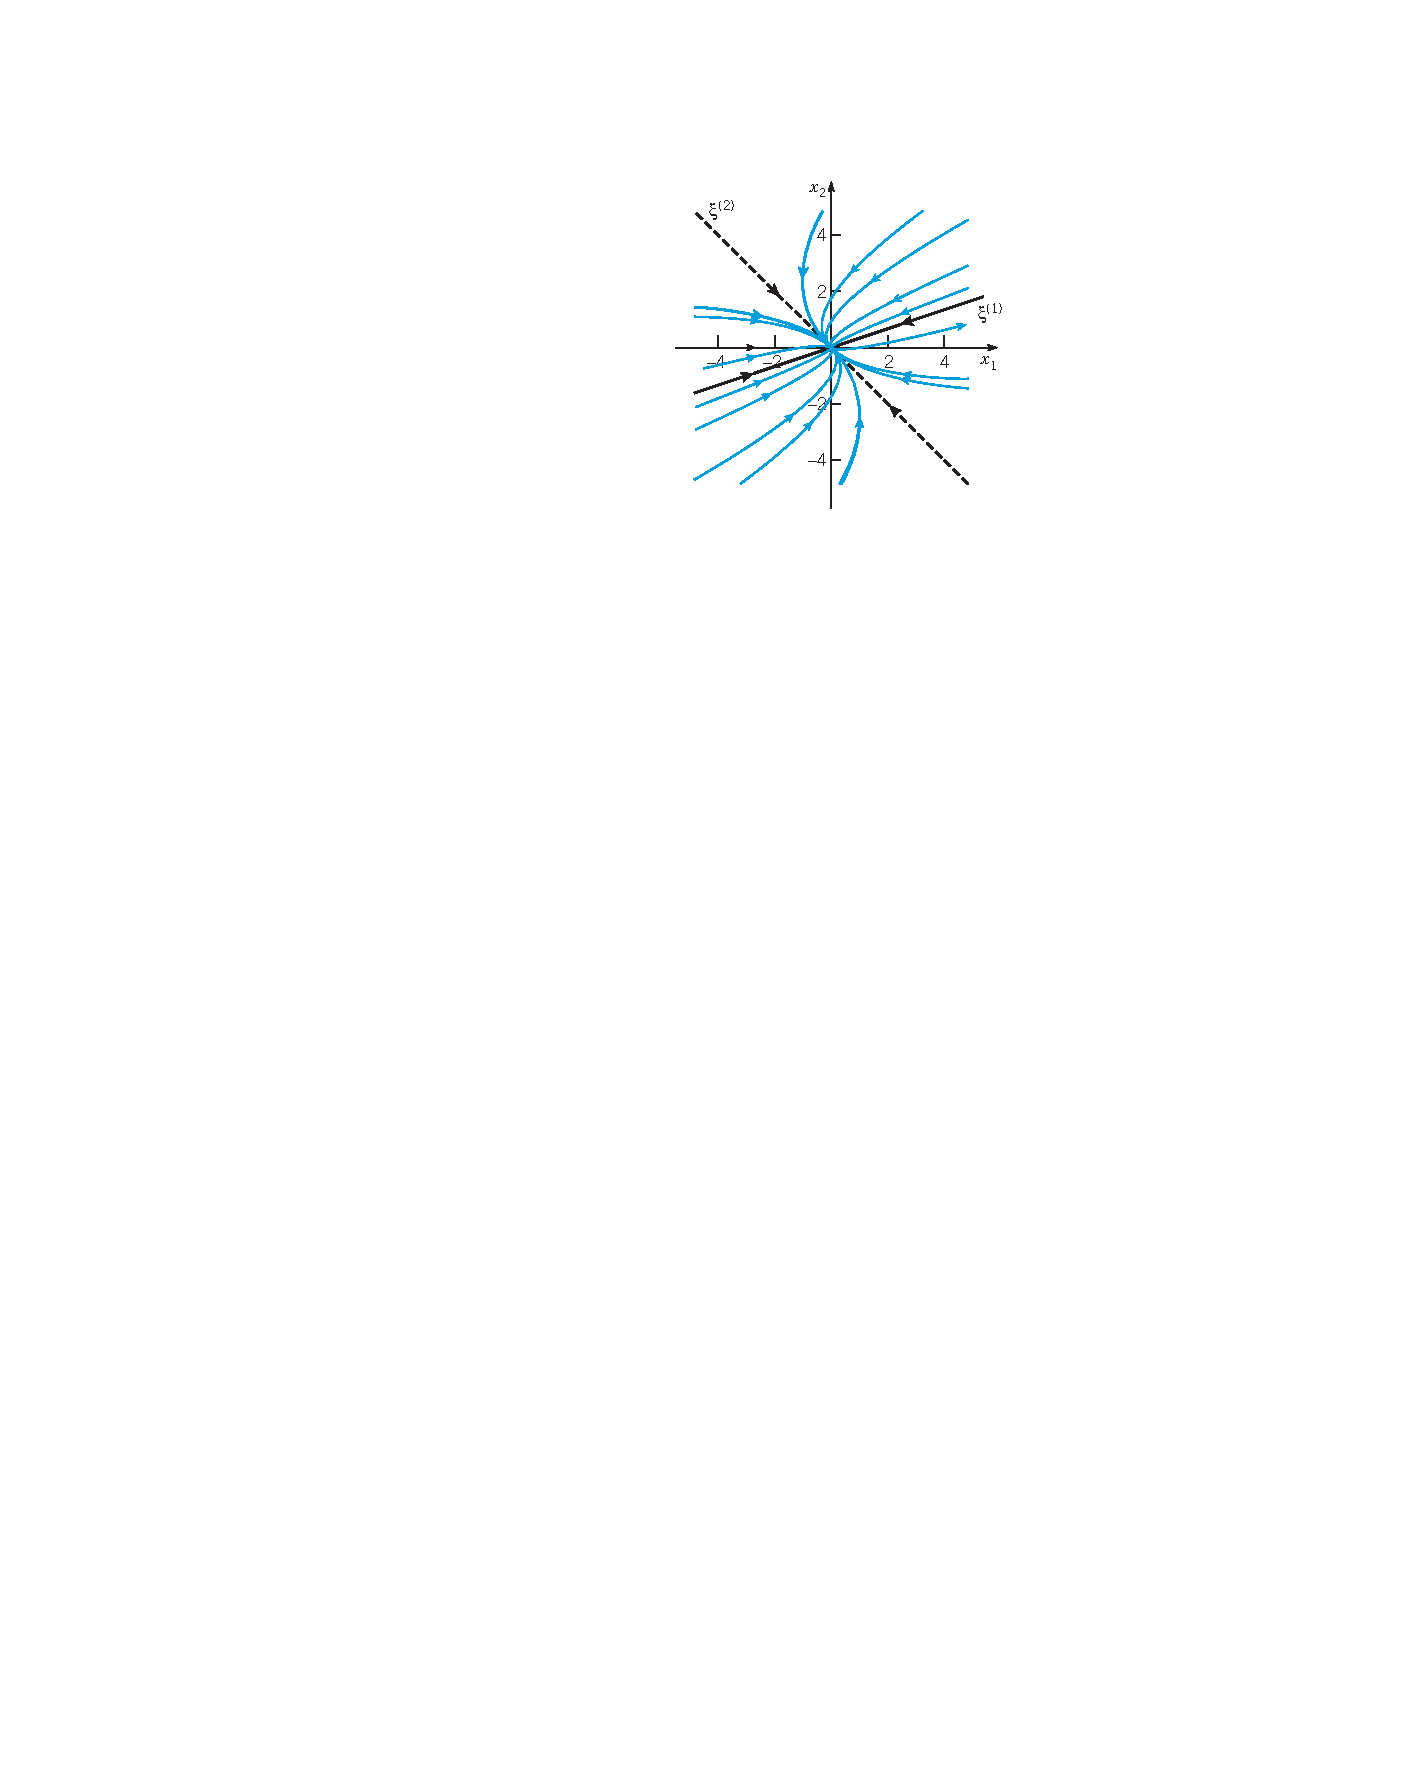
\includegraphics[width=0.5\textwidth]{Trajectories/1.pdf}
		\caption{Trajectories in the phase plane when the origin is a node (nodal sink) with $r_1 < r_2 < 0$. The solid black and dashed black curves show the fundamental solutions $\xib^{(1)}e^{r_1t}$ and $\xib^{(2)}e^{r_2t}$, respectively \cite[Figure 9.1.1]{boyce}.}
		\label{fig:trajectory1}
	\end{figure}
	
	\begin{figure}[H]
		\centering
		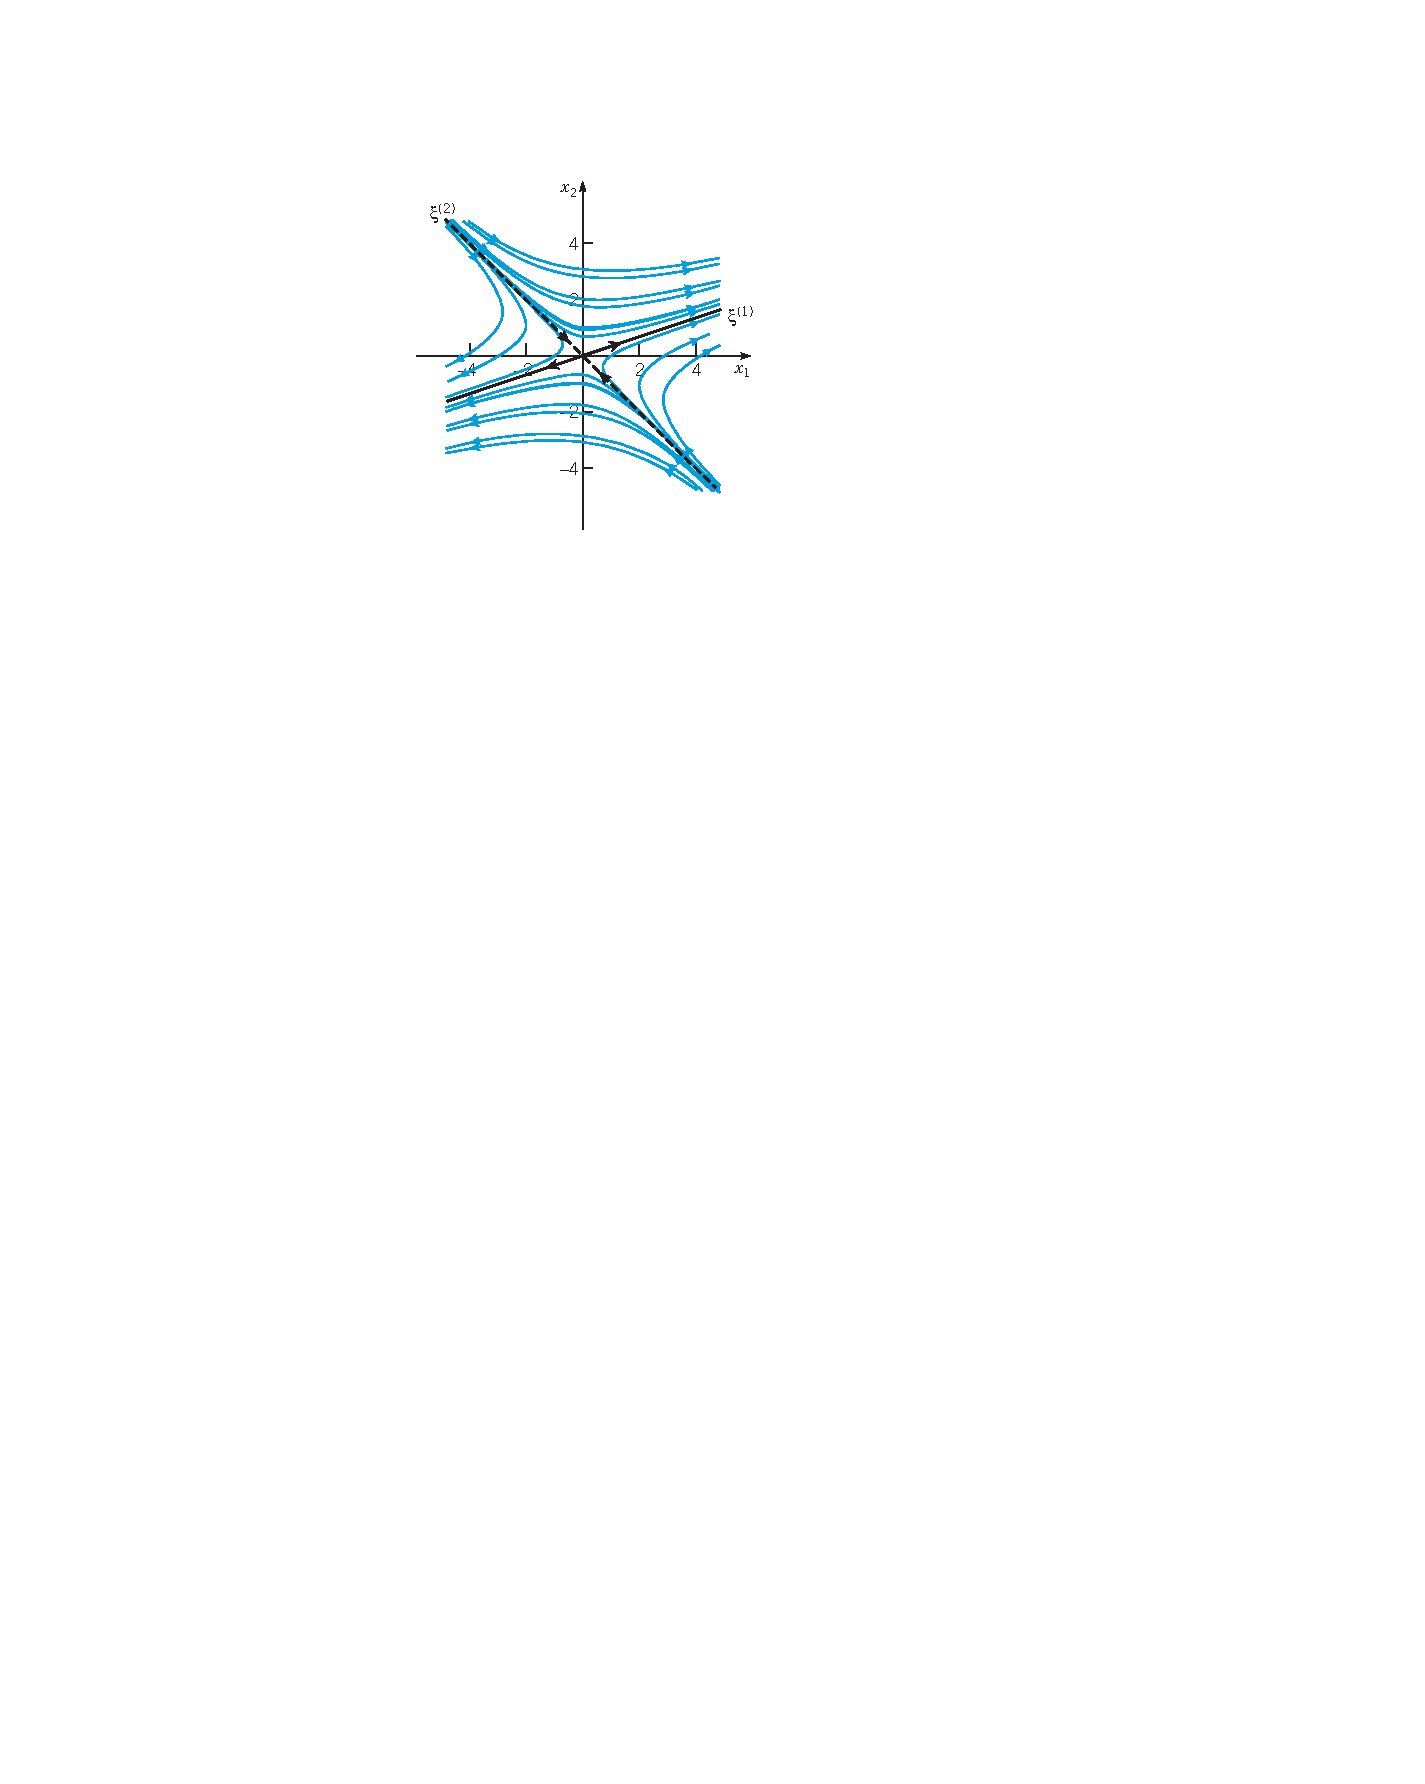
\includegraphics[width=0.53\textwidth]{Trajectories/2.pdf}
		\caption{Trajectories in the phase plane when the origin is a saddle point with $r_2 < 0 < r_1$. Note that the trajectories along one of the eigenvectors approach zero (this is the eigenvector associated with the negative eigenvalue), while those along the other eigenvector tend to $\infty$. \cite[Figure 9.1.2]{boyce}.}
		\label{fig:trajectory2}
	\end{figure}
	
	\item Case 2: Complex Eigenvalues of the form $r = \lambda \pm i \mu$ ($\mu>0$):
	
	A system with these eigenvalues can be transformed into the system:
	\begin{equation}\label{3.6}
		\xtp = \mat{ \lambda & \mu \\ -\mu & \lambda} \xt
	\end{equation} 
	and the solution to this system is given by:
	\[
		\xt = c_1 e^{\lambda t} \mat{\cos{\mu t} \\ -\sin{\mu t}} + c_2 e^{\lambda t} \mat{\sin{\mu t} \\ \cos{\mu t}} 
	\]
	as seen in \Cref{sec:complexeigs}. We now consider the following two subcases: 
	\begin{enumerate}[label=(\roman*)]
		\item $\lambda \neq 0$: \\ 
		From \Cref{3.6}, we have 
		\begin{align*}
			x' &= \lambda x + \mu y \\
			y' &= -\mu x + \lambda y
		\end{align*}
		Changing to polar coordinates, let $x= r \cos{\theta}, y = r \sin{\theta}$. Differentiating $x,y$ and Substituting the $x,y$ values into the equations above, we get: 
		\begin{equation}\label{eq3.7}
			x' = r'\cos{\theta} - r\theta'\sin{\theta} = \lambda r \cos{\theta} + \mu r\sin{\theta}
		\end{equation}
		\begin{equation}\label{eq3.8}
			y' = r'\sin{\theta} + r\theta'\cos{\theta} = -\mu r \cos{\theta} + \lambda r\sin{\theta}
		\end{equation}
		Multiplying \Cref{eq3.7} by $\cos{\theta}$ and \Cref{eq3.8} by $\sin{\theta}$, and adding the two equations, we get: 
		\[
		r' = \lambda r
		\]
		Multiplying \Cref{eq3.7} by $-\sin{\theta}$ and \Cref{eq3.8} by $\cos{\theta}$, and adding the two equations, we get: 
		\[
		\theta' = -\mu
		\]
		As $t \to \infty$, $r \to 0$ if $\lambda<0$ and $r \to \infty$ if $\lambda>0$. 
		The critical point in this case is a \vb{spiral sink} (\vb{stable focus}) when $\lambda<0$ and \vb{spiral source} (\vb{unstable focus}) when $\lambda>0$ (see \Cref{fig:trajectory5}). 
		% Since $\theta' = -\mu$, if $\mu>0$ then $\theta$ decreases as $t$ evolves and the motion is clockwise; if $\mu<0$ the trajectories are traversed anticlockwise.
		
		\item $\lambda = 0$: \\
		With the equations in subcase (i) holding, we now have that $r'=0 \implies r$ is constant so the trajectories are circles in the transformed coordinates. It can be shown that the trajectories are ellipses in the original coordinates, so the critical point in this case is a \vb{centre}, as in \Cref{fig:trajectory6}.
	\end{enumerate}

	To determine whether motion is clockwise or anticlockwise, we must look to the original linear system,
	\[
		\xtp = \mat{a & b \\ c & d}\xt.
	\]
	If $b-c>0$, the motion is clockwise; if $b-c<0$, the motion is anticlockwise.
	
	\begin{figure}[h!]
		\centering
		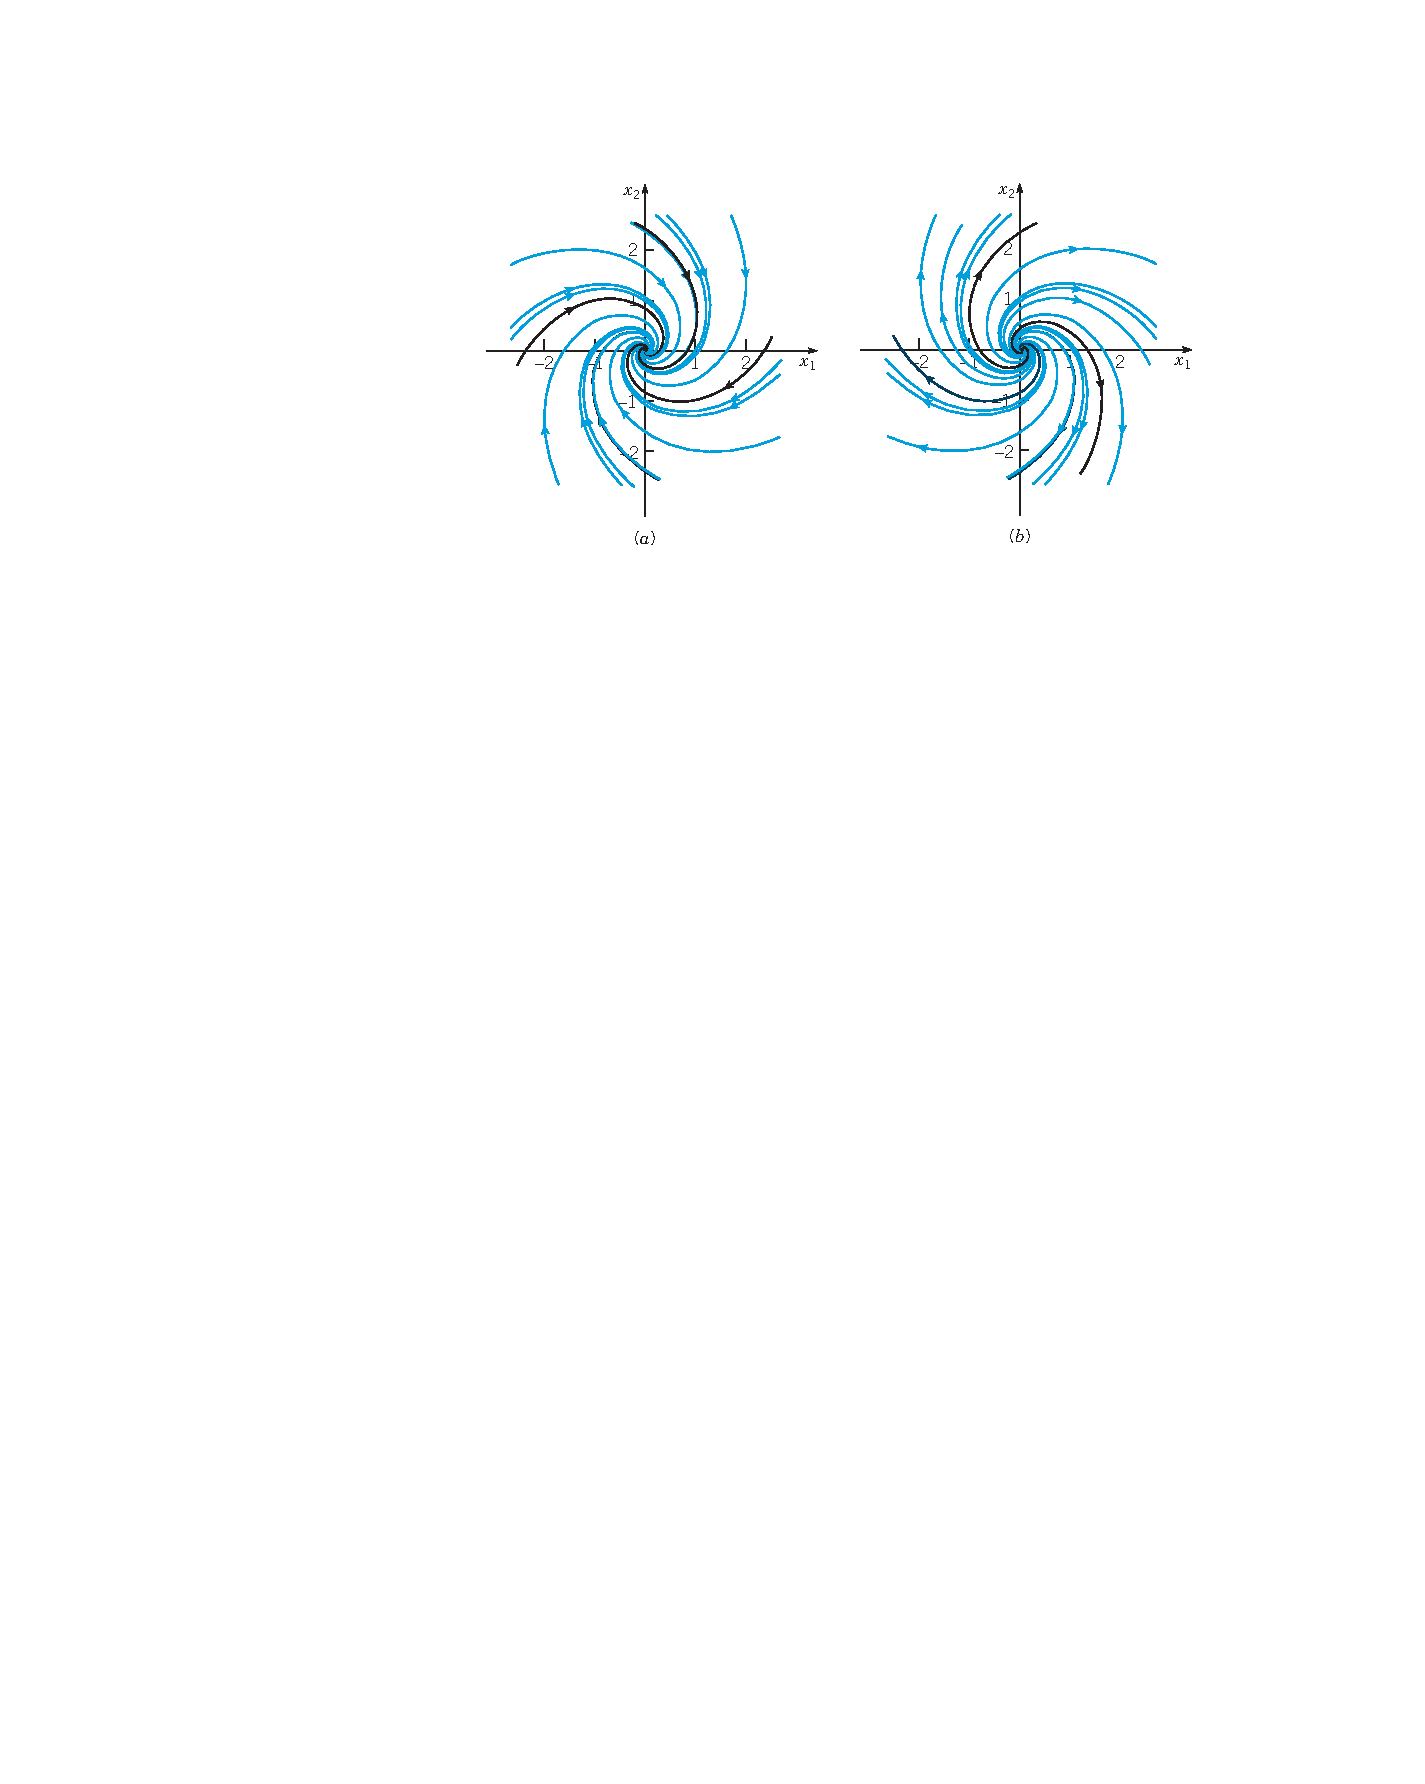
\includegraphics[width=0.8\textwidth]{Trajectories/5.pdf}
		\caption{Trajectories in the phase plane for a linear system with eigenvalues $\lambda \pm i\mu$, where the origin is (a) a spiral sink with $\lambda <0$ and (b) a spiral source with $\lambda >0$ \cite[Figure 9.1.5]{boyce}.}
		\label{fig:trajectory5}
	\end{figure}
	
	\begin{figure}[h!]
		\centering
		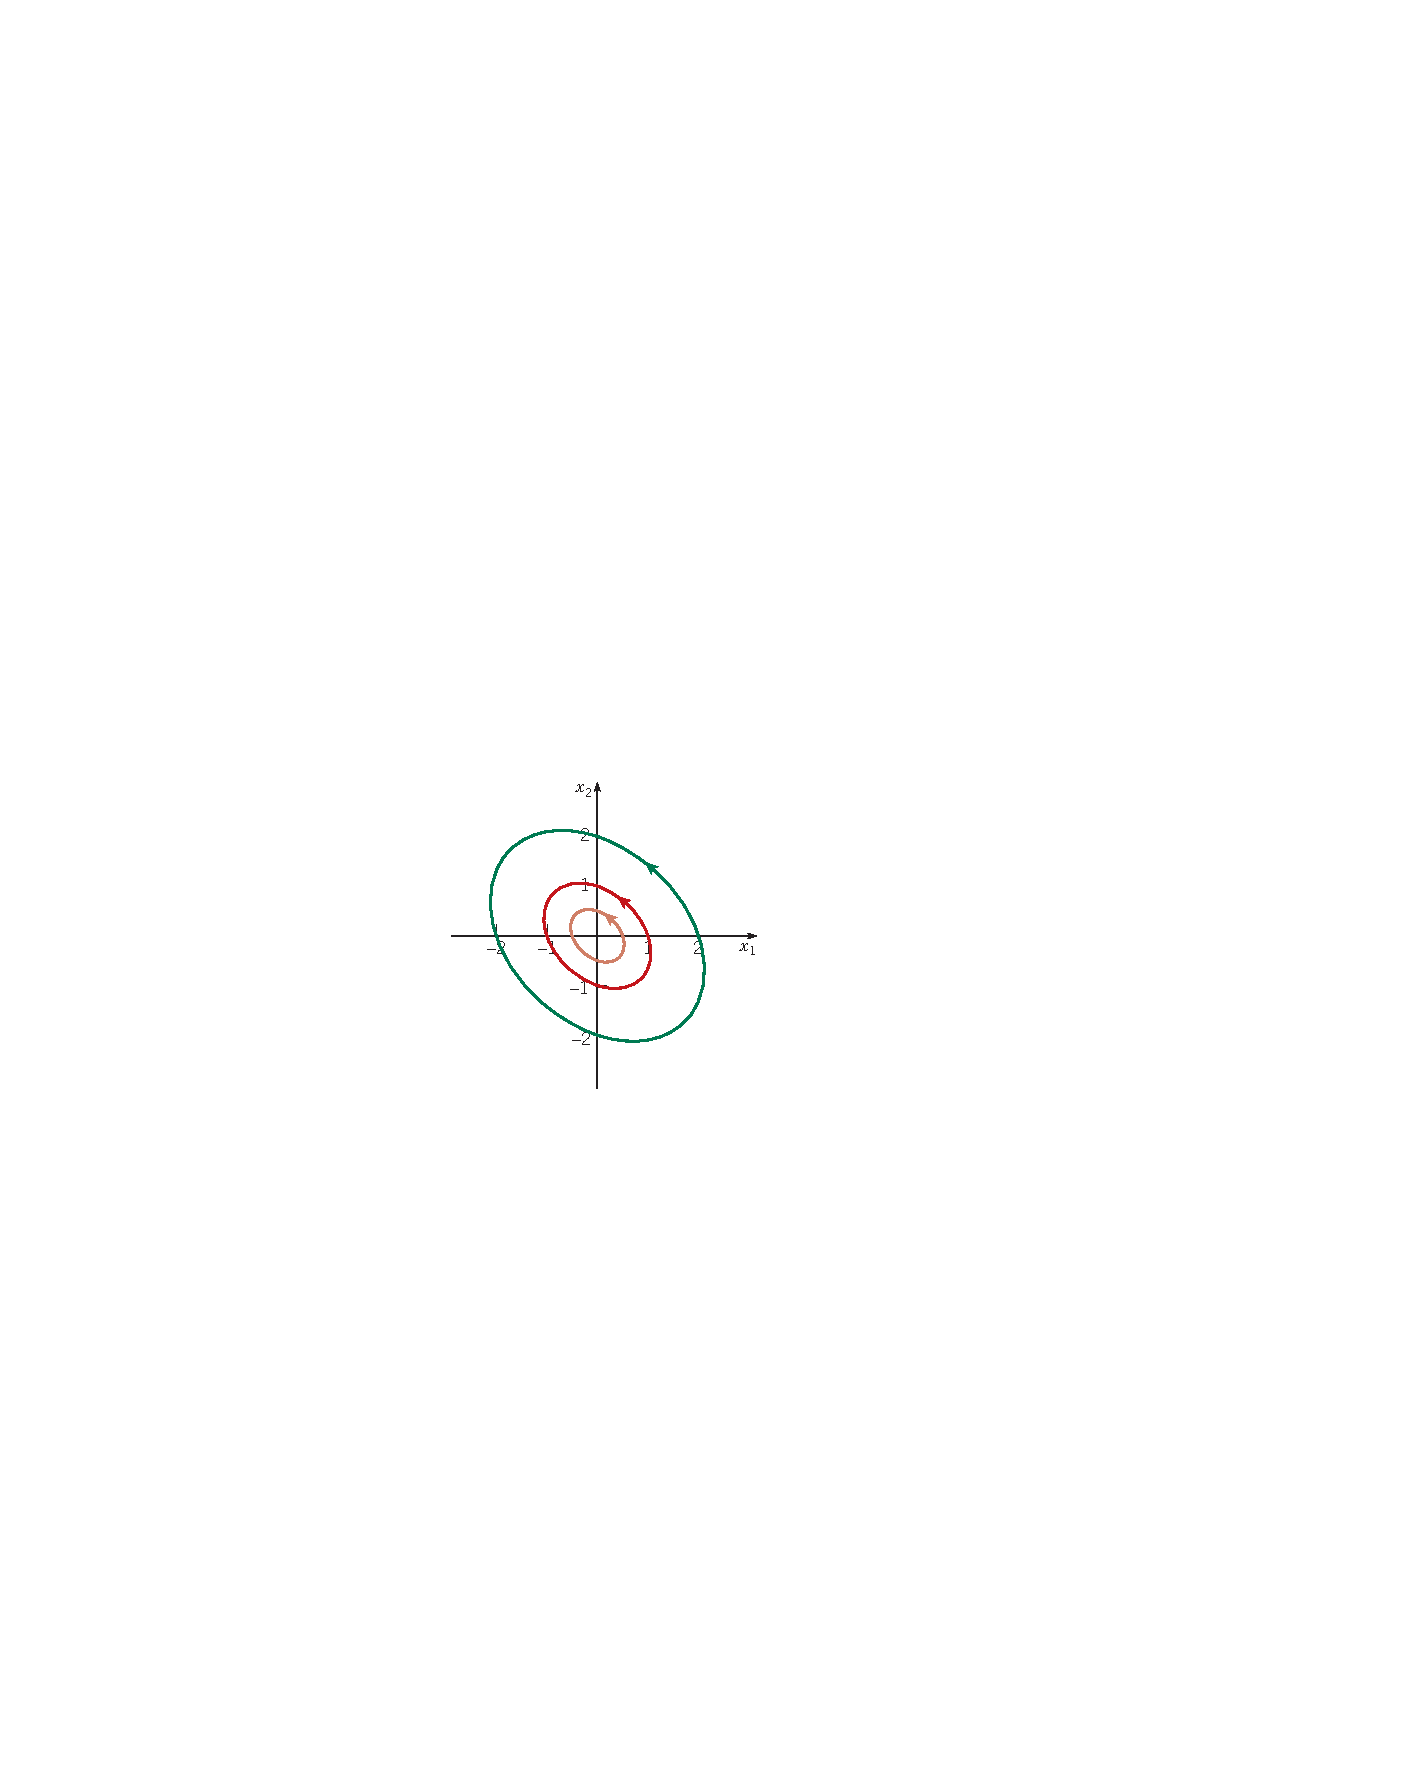
\includegraphics[width=0.5\textwidth]{Trajectories/6.pdf}
		\caption{Trajectories in the phase plane for a linear system with eigenvalues $\pm i\mu$, where the origin is a centre \cite[Figure 9.1.6(a)]{boyce}.}
		\label{fig:trajectory6}
	\end{figure}
	
	\item Case 3: Real and Equal Eigenvalues $r_1 = r_2 = r < 0$:
	
	For cases with repeated eigenvalues, recall that as seen in \Cref{sec:repeatedeigs}, we can either have 2 or 1 linearly independent eigenvectors associated with $r$ depending on the geometric multiplicities of the eigenvalues. We consider the following two subcases:
	\begin{enumerate}[label=(\roman*)]
		\item Two linearly independent eigenvectors: \\ 
		The solution is given by 
		\[
		\xt = c_1 e^{rt} \xib_1 + c_2 e^{rt} \xib_2
		\]
		The ratio $\frac{x}{y}$ is independent of $t$ but depends on the components of $\xib_1$ and $\xib_2$ and on $c_1, c_2$. Thus every trajectory lies on a straight line through the origin and since $r<0$, the trajectories approach the critical point as $t \to \infty$. The critical point in this case is a \vb{proper node} (\vb{star point}) (see \Cref{fig:trajectory3}).
		
		\item One linearly independent eigenvector: \\
		The solution is given by 
		\[
		\xt = c_1 e^{rt} \xib + c_2 e^{rt} (\xib t + \etab)
		\]
		Since $r<0$, the trajectories approach the critical point. As $t \to \infty$, the trajectory is dominated by $\xib$ (if $c_2 \neq 0$, the $c_2 te^{rt} \xib$ term dominates; if $c_2 = 0$ then $c_1 e^{rt} \xib$ dominates) so approaches the origin tangent to the line through this eigenvector. The critical point in this case is an \vb{improper node}, or \vb{degenerate node} (see \Cref{fig:trajectory4}).
		
		As in the case for complex eigenvalues, if $b-c>0$, the motion is clockwise; if $b-c<0$, the motion is anticlockwise.\footnote{If $b-c=0$, the critical point cannot be a spiral, centre, or improper node.}
	\end{enumerate}
	If instead the eigenvalues are positive, $r_1 = r_2 = r > 0$, the trajectories are similar but the direction of motion is reversed.
\end{itemize}

\begin{figure}[h!]
	\centering
	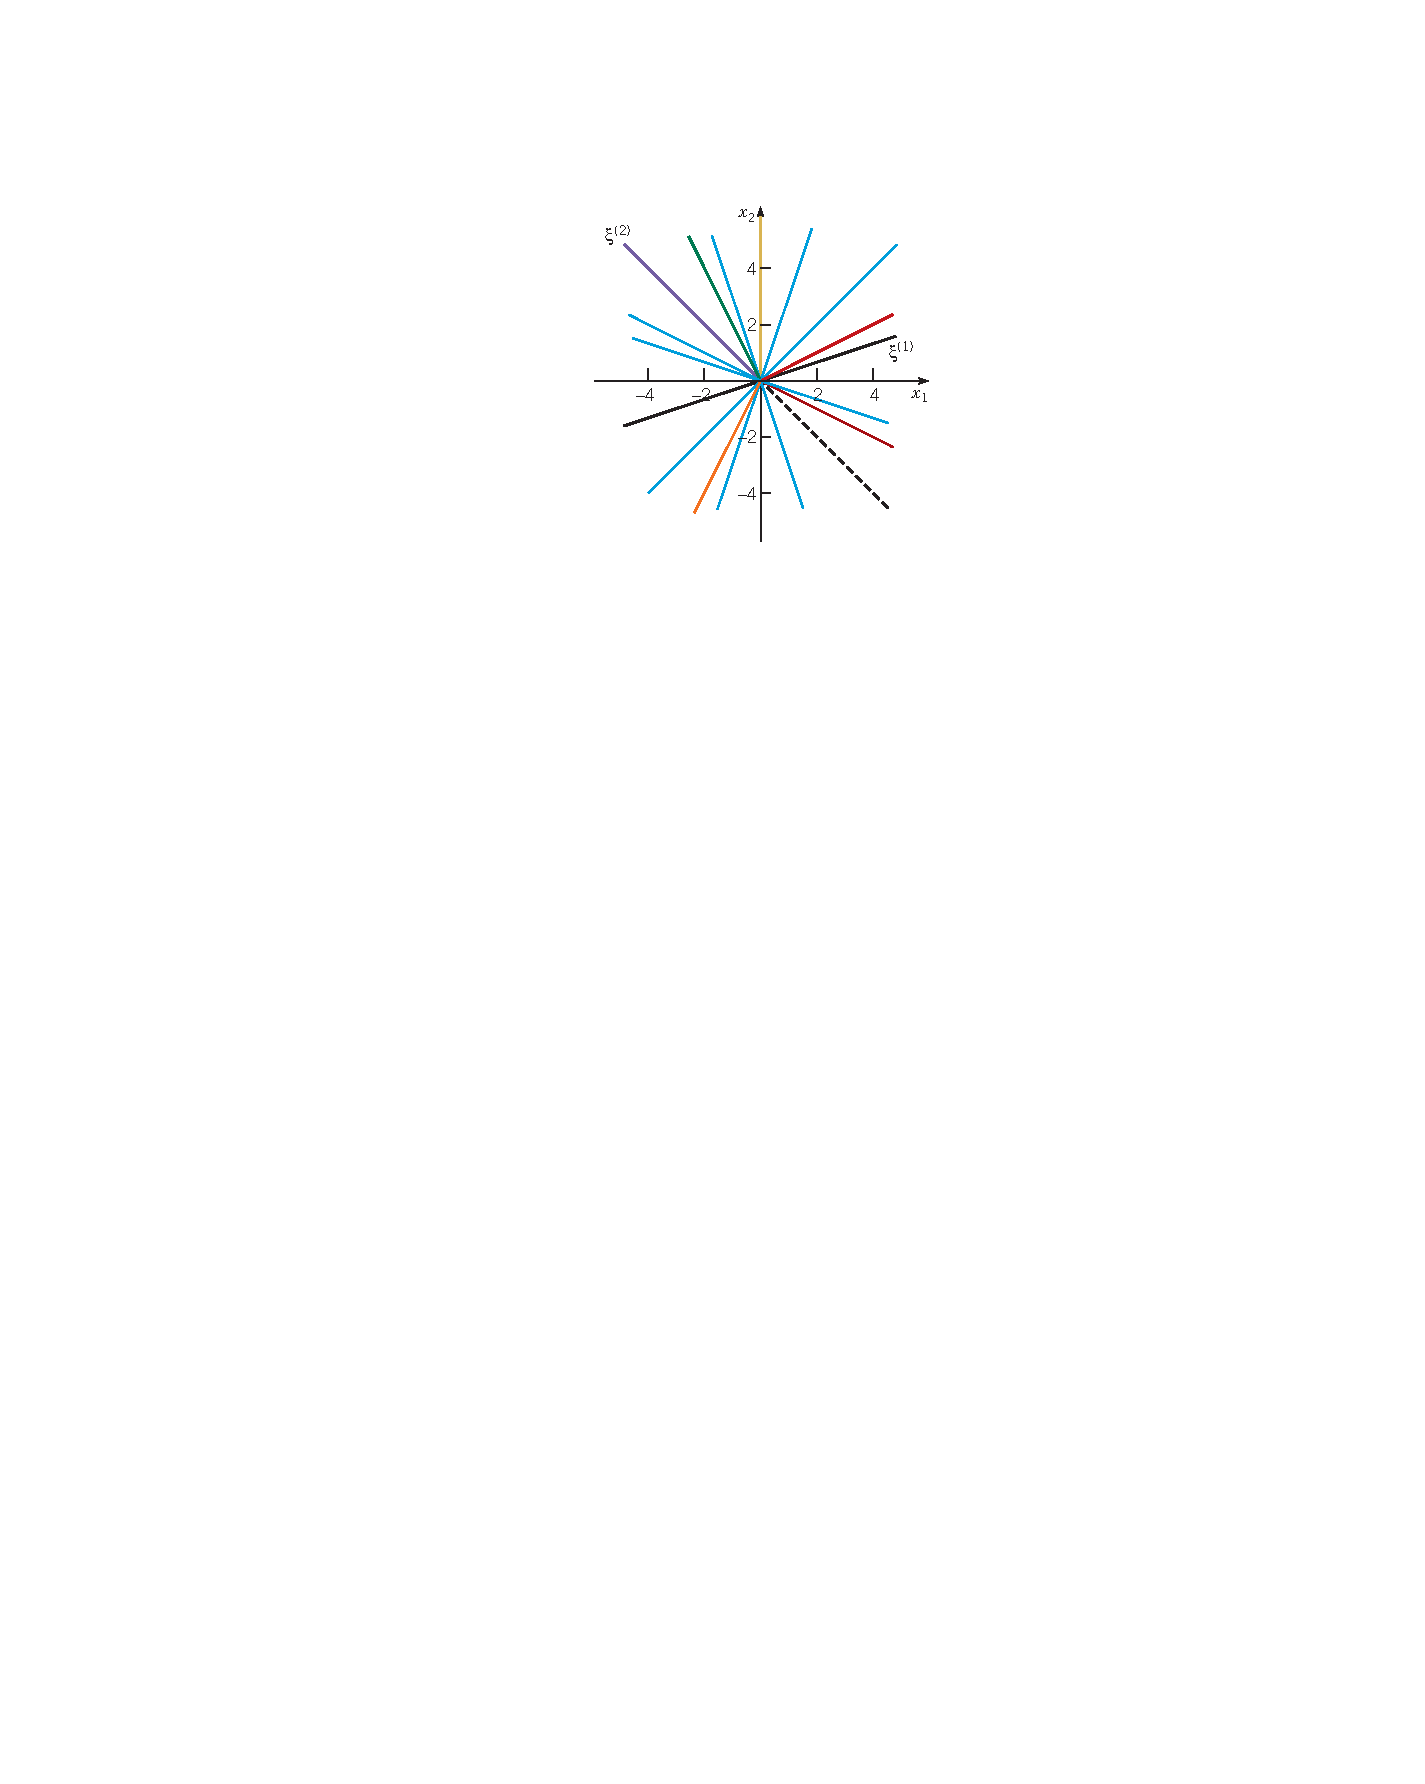
\includegraphics[width=0.5\textwidth]{Trajectories/3.pdf}
	\caption{Trajectories in the phase plane when the origin is a proper node with $r_1 = r_2 < 0$ \cite[Figure 9.1.3(a)]{boyce}.}
	\label{fig:trajectory3}
\end{figure}

\begin{figure}[h!]
	\centering
	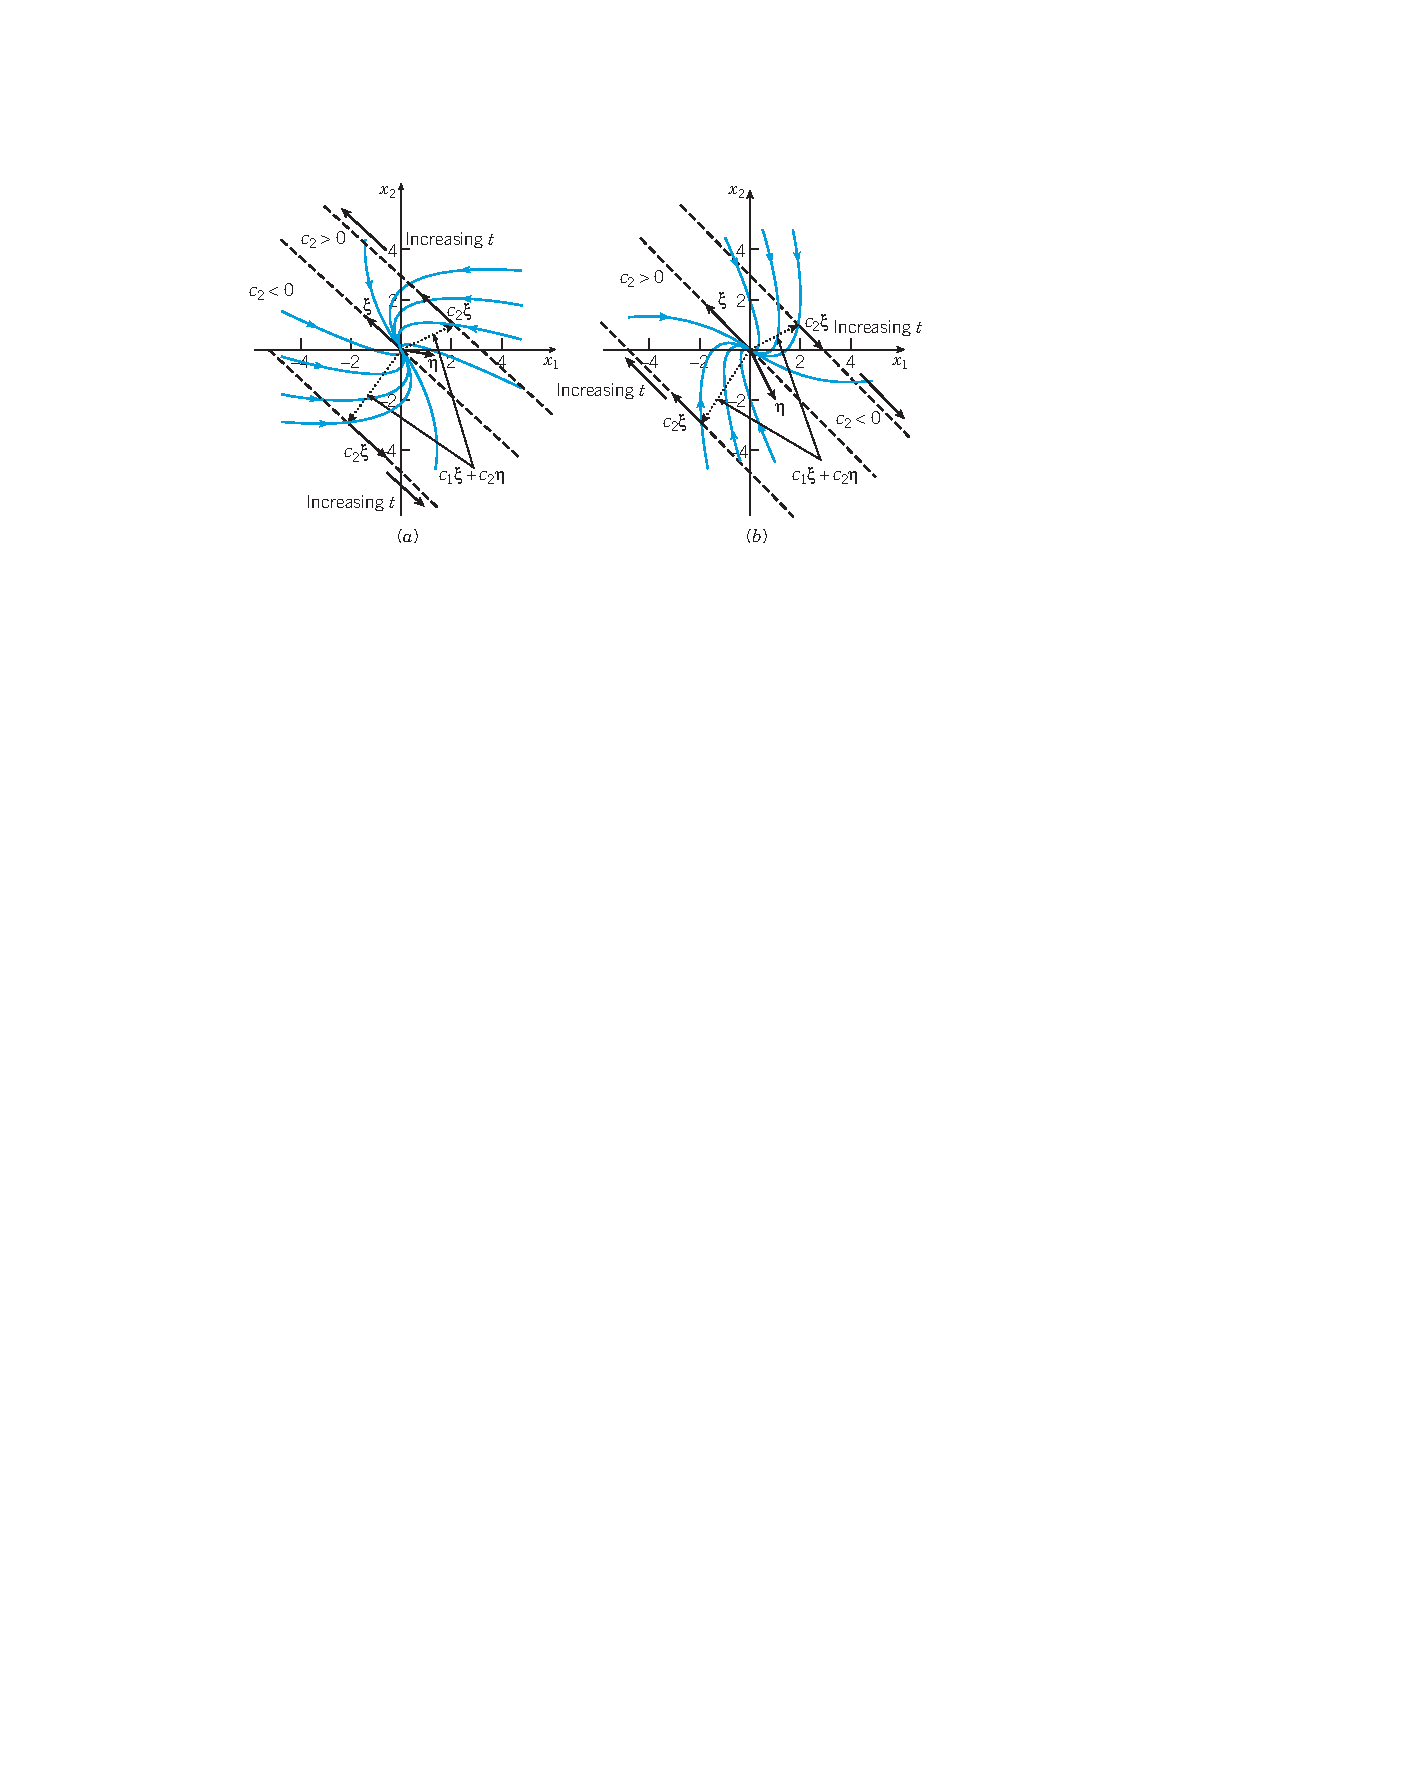
\includegraphics[width=0.8\textwidth]{Trajectories/4.pdf}
	\caption{Trajectories in the phase plane when the origin is (a) an improper node with eigenvalues $r_1 = r_2 < 0$ and one independent eigenvector $\xib$, and (b) the same but with a different generalised eigenvector $\etab$ \cite[Figure 9.1.4]{boyce}.}
	\label{fig:trajectory4}
\end{figure}

\subsection{Stability of Critical Points and Systems}

We know that if $\vbx(0) = \xta$, then $\xt = \xta$ for all $t$. Now we consider what happens to trajectories starting near $\xta$.

\begin{definition}
	A critical point $\xta$ is \vb{stable} if $\forall \varepsilon>0$, $\exists \delta>0$ such that $|\vbx(0) - \xta| < \delta$ implies $|\xt - \xta|<\varepsilon$ for all $t>0$.
\end{definition}

\begin{definition}
	A critical point $\xta$ that is not stable is called unstable.
\end{definition}

\begin{definition}
	A critical point $\xta$ is \vb{asymptotically stable} if it is stable and $\exists \delta_0 >0$ such that $|\vbx(0) - \xta| < \delta_0$ implies $|\xt - \xta|<\varepsilon$ as $t \to \infty$.
\end{definition}

Intuitively, a critical point being stable means that, starting from a point close to the critical point, the trajectory remains close to the point. A CP being asymptotically stable means that, starting close to the CP, the trajectory will tend towards the critical point.

A graphical representation of stability and asymptotic stability is given in \Cref{fig:stability}.

\begin{figure}[!ht]
	\centering
	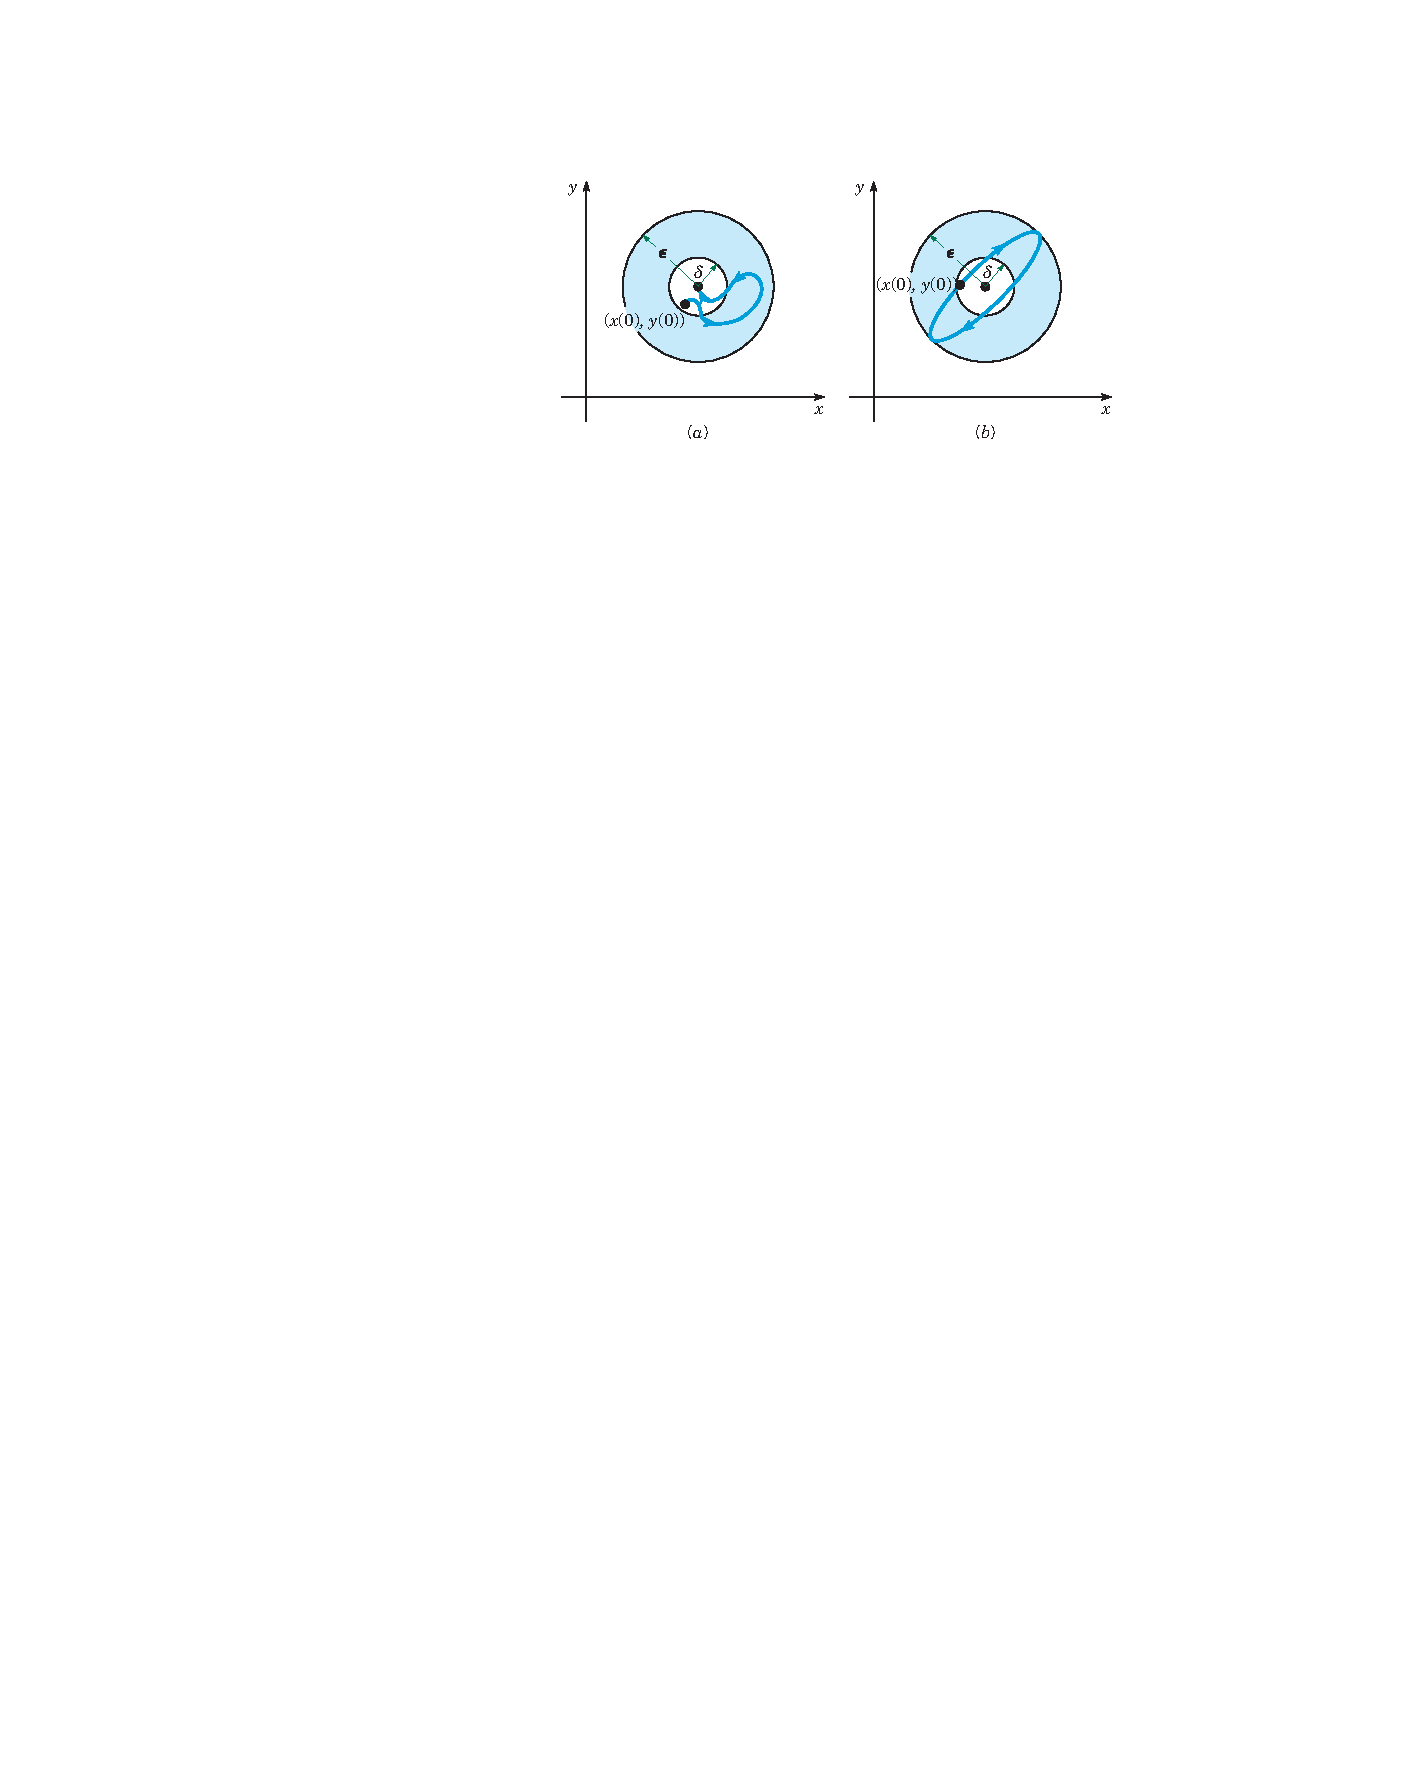
\includegraphics[width=0.75\textwidth]{stability.pdf}
	\caption{Graphical representation of trajectories that exhibit (a) asymptotic stability and (b) stability \cite[Figure 9.2.1]{boyce}.}
	\label{fig:stability}
\end{figure}

\subsubsection{Stability of Linear Systems}

We already know that for a linear system $\xtp = A\xt$, the solution is given by
\[
\xt = c_1e^{r_1t}\xib_1 + c_2e^{r_2t}\xib_2,
\]
and a critical point is $\xta = (0,0)$.

Stability for a linear system depends on the sign of the eigenvalues:
\begin{itemize}
	\item If $\Re(r_1) \leq 0$ and $\Re(r_2) \leq 0$, this implies that the linear system is stable as trajectories will return to the origin (or, at the very least, the trajectories will not go away from the origin) as $e^{r_1t}$ and $e^{r_2t}$ decay.
	\item If $\Re(r_1)<0$ and $\Re(r_2)<0$, the system is asymptotically stable.
	\item If $\Re(r_1)>0$ or $\Re(r_2)>0$, the system is unstable.
\end{itemize}

\Cref{table:stability} summarises the stability and type of critical point for a linear system depending on its eigenvalues.

\begin{table}[H]
	\begin{center}
		\begin{tabular}{c|c|c}
			Eigenvalues & Critical Points & Stability \\
			\hline
			$r_1 > r_2 > 0$ & Node (nodal source) & Unstable \\
			$r_1 < r_2 < 0$ & Node (nodal sink) & Asymptotically stable \\
			$r_2 < 0 < r_1$ & Saddle point & Unstable \\
			$r_1 = r_2 > 0$ & Proper/improper node & Unstable \\
			$r_1 = r_2 < 0$ & Proper/improper node & Asymptotically stable \\
			$r_1,r_2 = \lambda \pm i\mu$, $\lambda>0$ & Focus/spiral source & Unstable \\
			$r_1,r_2 = \lambda \pm i\mu$, $\lambda<0$ & Focus/spiral sink & Asymptotically stable \\
			$r_1,r_2 = \pm i\mu$ & Centre & Stable \\
		\end{tabular}
	\end{center}
	\caption{Classification of nature and stability of critical points of a linear system.}
	\label{table:stability}
\end{table}

\subsubsection{Stability of Non-linear Systems}

As we saw in \Cref{sec:linearapproxcp}, given a system described by
\[
\begin{cases}
	x' = F(x,y) \\
	y' = G(x,y)
\end{cases}
\]
we can transform it into a system of ODEs of the form
\[
\mat{u'\\v'} = \underbrace{\mat{\p_x F(\xta) & \p_y F(\xta) \\ \p_x G(\xta) & \p_y G(\xta)}}_{\text{Jacobian}} \mat{u\\v} + \underbrace{\mat{\eta_1 \\ \eta_2}}_{\text{Perturbation}}
\]
which becomes a linear system if we ignore the perturbation $\mat{\eta_1 \\ \eta_2}$.

It is tempting to make conclusions on the stability of the non-linear system based on the behaviour of the linearised system. This is valid, \emph{except for} the centre, as the following example illustrates.

\begin{eg}\label{eg:centrecp}
	Consider the non-linear system described by the equations
	\begin{align*}
		x' &= -y + x(x^2+y^2) \\
		y' &= x + y(x^2+y^2).
	\end{align*}
	It is easy to see that $x'=y'=0$ at the point $(0,0)$, thus we have a critical point $\xta = (0,0)$.
	
	Now we find the Jacobian matrix:
	\begin{equation*}
		\begin{alignedat}{3}
			\p_x F &= (x^2+y^2) + 2x^2 &&= 0 &\text{ at } (0,0) \\
			\p_y F &= -1 + 2xy &&= -1 &\text{ at } (0,0) \\
			\p_x G &= 1 + 2xy &&= 1 &\text{ at } (0,0) \\
			\p_y G &= (x^2+y^2) + 2y^2 &&= 0 &\text{ at } (0,0) \\
		\end{alignedat}
	\end{equation*}
	Thus
	\[
	J = \mat{0 & -1 \\ 1 & 0}.
	\]
	We find the eigenvalues of $J$:
	\begin{align*}
		\det \mat{-r & -1 \\ 1 & -r} &= 0 \\
		r^2 + 1 &= 0 \\
		r &= \pm i.
	\end{align*}
	From \Cref{table:stability}, this critical point is a centre. To determine the stability of the critical point from the original equations, we convert to polar coordinates, setting $x=r\cos\theta$ and $y=r\sin\theta$. Then
	\begin{equation}\label{eq:polareg1}
		x' = r'\cos{\theta} - r\theta'\sin{\theta} = -r\sin\theta + r^3\cos\theta,
	\end{equation}
	\begin{equation}\label{eq:polareg2}
		y' = r'\sin{\theta} + r\theta'\cos{\theta} = r\cos\theta + r^3\sin\theta.
	\end{equation}
	
	Multiplying \Cref{eq:polareg1} by $\cos{\theta}$ and \Cref{eq:polareg2} by $\sin{\theta}$, and adding the two equations, we get: 
	\[
	r' = r^3.
	\]
	Multiplying \Cref{eq:polareg1} by $-\sin{\theta}$ and \Cref{eq:polareg2} by $\cos{\theta}$, and adding the two equations, we get: 
	\[
	\theta' = 1.
	\]
	
	From these transformed equations, we see that starting from some $r\neq 0$ (i.e. a point near the critical point at the origin), the value of $r$ is always increasing, thus with $\theta'=1$ also, the CP is a spiral and thus unstable.
	
	This is a very different result to what we would have concluded from studying the linearised system - the CP is an unstable spiral instead of a stable centre.
\end{eg}

\begin{remark}
	For centres, we cannot determine the stability of the critical point simply by looking at the linearised system.
\end{remark}

\begin{figure}[!ht]
	\centering
	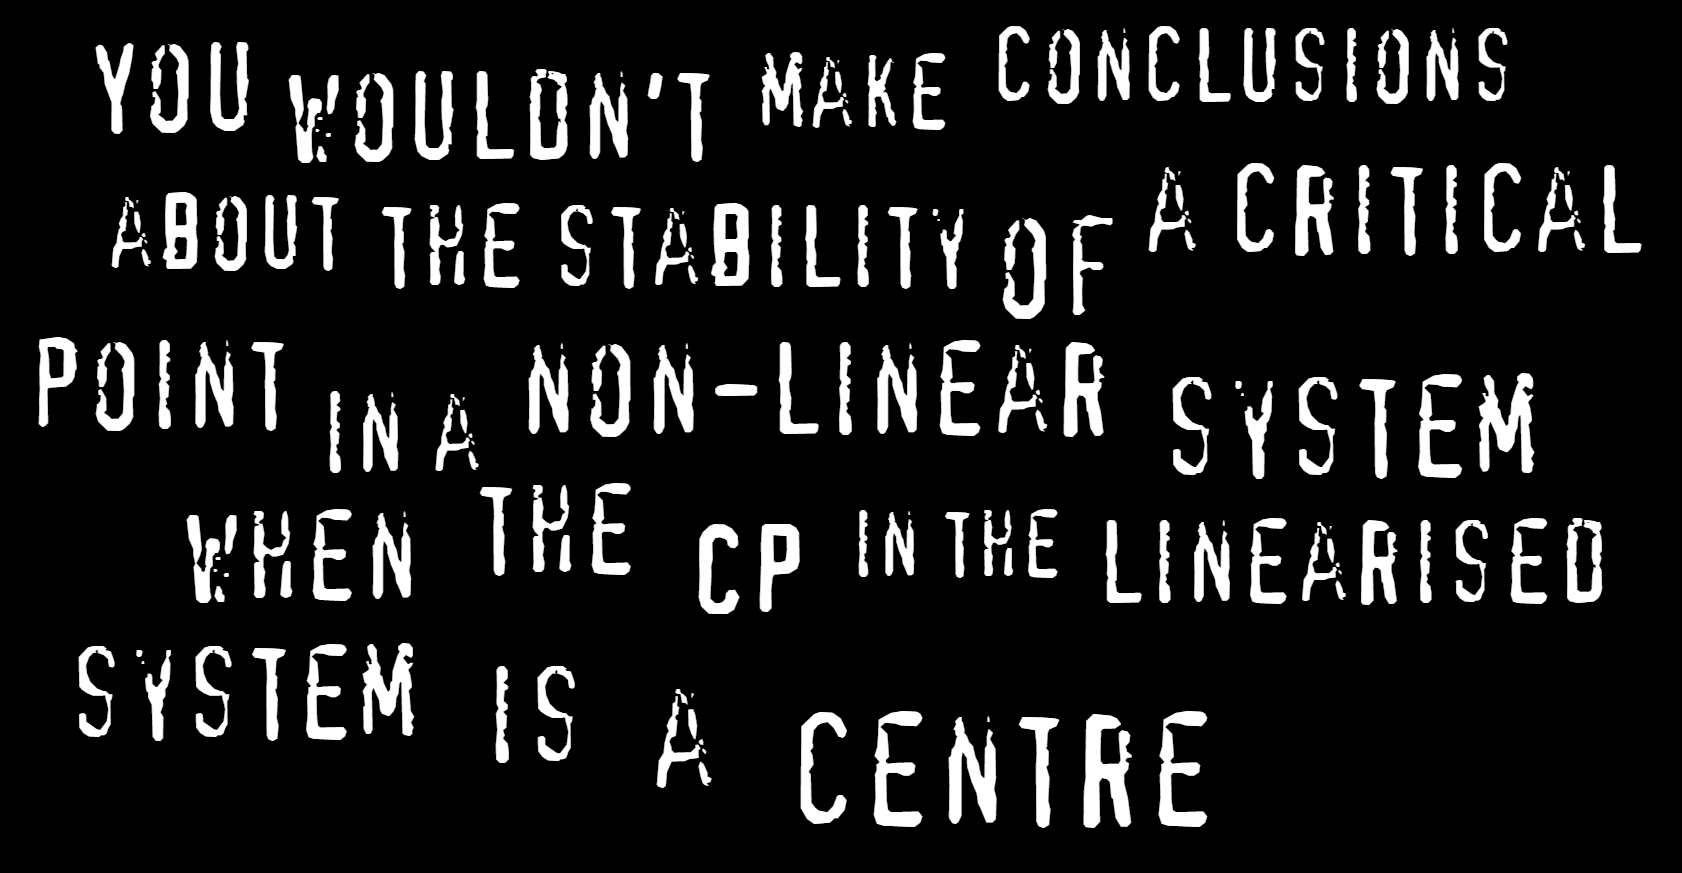
\includegraphics[width=0.65\textwidth]{Centre.png}
	\label{fig:centrepiracy}
\end{figure}

\begin{eg}[Damped Pendulum]\label{eg:dampedpendulum2}
	We continue the work started in \Cref{eg:dampedpendulum}, we have the following system describing the motion of the pendulum, 
	\begin{align*}
		x' &= y \\
		y' &= -\omega^2 \sin{x} - \gamma y,
	\end{align*}
	critical points at
	\[
	(x,y) = (n\pi, 0),
	\]
	and the Jacobian given by
	\[
	J(n\pi,0) = \mat{0 & 1 \\ \omega^2 (-1)^{n+1} & -\gamma}.
	\]
	
	We find the eigenvalues of the Jacobian matrix:
	\begin{align*}
		r(r+\gamma) + \omega^2 (-1)^n &= 0 \\
		r_{\pm} &= \frac{-\gamma \pm \sqrt{\gamma^2 - 4(-1)^n\omega^2}}{2}.
	\end{align*}
	
	In the case that $n$ is even, and assuming that $\gamma < 2\omega$ (i.e. $\gamma^2 < 4\omega^2$) so that the system is only lightly damped, the eigenvalues are
	\[
	r_{\pm} = \frac{-\gamma \pm i\sqrt{4\omega^2 - \gamma^2}}{2},
	\]
	so we have complex eigenvalues with $\lambda<0$. Thus from \Cref{table:stability}, the CP is a spiral sink, or stable focus.
	
	To determine whether this spiral is clockwise or anticlockwise, choose a point with $y=0$ and small $x>0$, then $y'<0$ so the spiral is clockwise. The same applies to all critical points $(n\pi, 0)$ with $n$ even.
	
	Now for the case with $n$ odd,
	\[
	r_{\pm} = \frac{-\gamma \pm \sqrt{\gamma^2 + 4\omega^2}}{2},
	\]
	so $r_+>0$ and $r_-<0$. Thus this is a saddle point.
	
	Finally, we find the eigenvectors associated with these eigenvalues as $\mat{1\\r_+}$ and $\mat{1\\r_-}$. Therefore, the general solution is
	\[
	\mat{u\\v} = c_1e^{r_+t}\mat{1\\r_+} + c_2e^{r_-t}\mat{1\\r_-}.
	\]
	For the part of the saddle point trajectories that converge to zero, the solution must correspond to $c_1=0$ since $r_+>0$. In thus case, $\frac{u}{v} = \frac{1}{r_-} < 0$, thus there trajectories are downward sloping. For the trajectories `exiting' the saddle point, $\frac{u}{v} > 0$ so the lines are upward sloping.
	
	Putting together what we have found in this example, the phase portrait for the damped pendulum is shown in \Cref{fig:pendulumportrait}. The \vb{basin of attraction} is the shaded region, where all initial conditions in this region have trajectories that converge to the critical point $(0,0)$ (geometrically, this corresponds to the pendulum hanging at rest at its lowermost position).
\end{eg}

\begin{figure}[!ht]
	\centering
	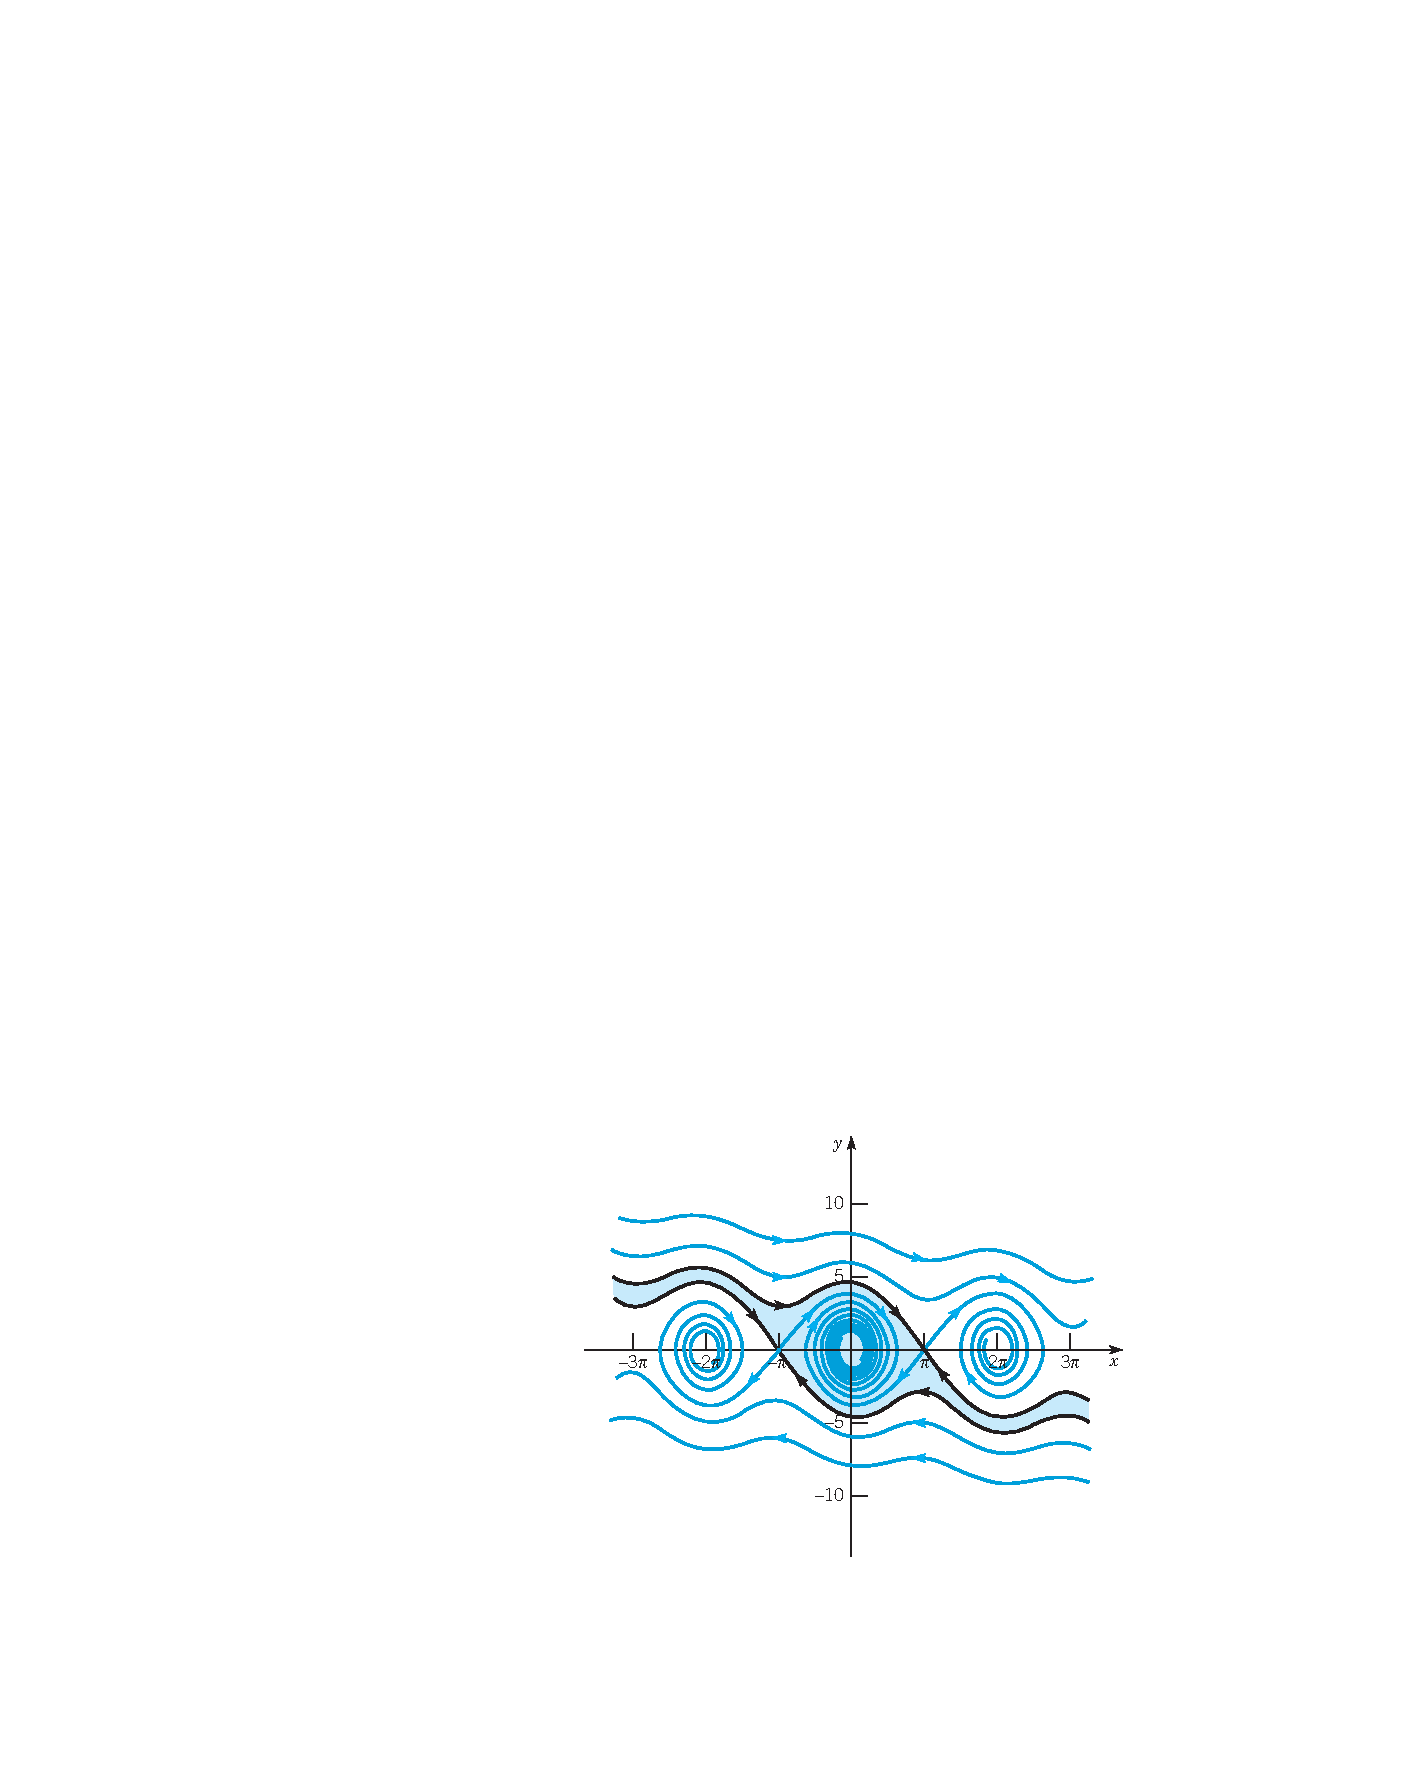
\includegraphics[width=0.75\textwidth]{PendulumPortrait.pdf}
	\caption{Phase portrait for the damped pendulum of Examples \ref{eg:dampedpendulum} and \ref{eg:dampedpendulum2}. The shaded region is the basin of attraction for the CP $(0,0)$ \cite[Figure 9.3.5]{boyce}.}
	\label{fig:pendulumportrait}
\end{figure}

\subsection{Implicit Trajectories}\label{sec:implicittraj}

Up to now, we've covered the local behaviour of the solutions to systems of ODEs. We now move on to the global behaviour of ODEs to draw the entire phase portrait for systems.

For some systems, the trajectories can be found in an implicit form $f(x,y) = c$, where $c$ is a constant.

\begin{eg}\label{eg:imptraj}
	Consider the following system:
	\begin{align*}
		x' &= 4 - 2y \\
		y' &= 12 - 3x^2
	\end{align*}
	First, we find the critical points where $x' = y' = 0$.
	\[
	4-2y = 0 = 12-3x^2 \implies y = 2 
	\] 
	and 
	\[
	x^2 = 4 \implies x = \pm 2
	\]
	Thus, the critical points are $(2,2)$ and $(2,-2)$.
	Then, the Jacobians for these points are given by:
	\begin{align*}
		J(x, y) &= \mat{0 & -2 \\ -6x & 0} \\
		J(2, 2) &= \mat{0 & -2 \\ -12 & 0} \\
		J(-2, 2) &= \mat{0 & -2 \\ 12 & 0} 
	\end{align*}
	For the Jacobian associated with $(2,2)$, the eigenvalues are found to be $r = \pm \sqrt{24}$. So $(2,2)$ is a saddle point.
	
	For the Jacobian associated with $(-2,2)$, the eigenvalues are found to be $r = \pm i\sqrt{24}$. So $(-2,2)$ is a centre.\footnote{In the linearisation of the system at least: recall that in the case that the CP of the local linear system is a centre, we cannot say that the CP in the non-linear system is.}
	
	We now wish to have a global picture of how these critical points emerge. Since $x$ and $y$ are functions of time, we can write $y$ as a function of $x$. Then, 
	\[
	\frac{dy}{dx} = \frac{\frac{dy}{dt}}{\frac{dx}{dt}} = \frac{y'}{x'} = \frac{12-3x^2}{4-2y}
	\]
	
	It is now easy to see that this system can be solved using the method of separation of variables as follows:
	\[
	(4-2y)\,dy = (12 - 3x^2)\,dx
	\]
	We now integrate both sides:
	\begin{align*}
		\int 4-2y\,dy &= \int 12 - 3x^2\,dx \\
		4y - y^2 &= 12x - x^3 + c
	\end{align*}
	which can be expressed implicitly as
	\[
	x^3 - y^2 - 12x + 4y = c
	\]
	This is now an implicit trajectory. By varying the value of $c$, we can get multiple trajectories to draw a phase portrait, as is done in \Cref{fig:implicittraj}.
\end{eg}

\begin{figure}[!ht]
	\centering
	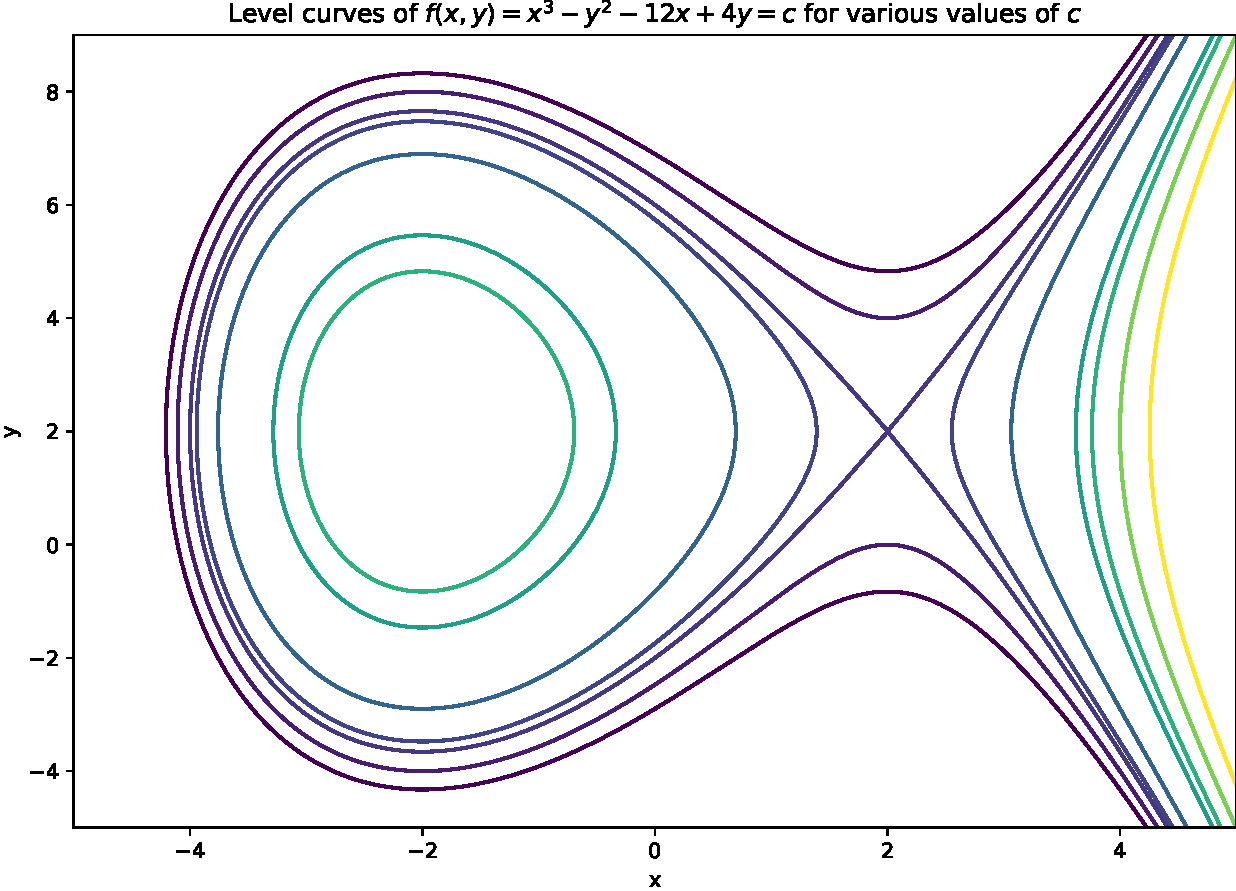
\includegraphics[width=0.75\textwidth]{implicitTrajectories.pdf}
	\caption{Phase portrait showing the implicit trajectories for the system in \Cref{eg:imptraj}. The level curve that intersects the saddle point forms a boundary between the trajectories that diverge as $t \to \pm \infty$ and those which are stable/periodic around the centre at $(-2,2)$. This curve (corresponding to $c=-12$) is called the separatrix.}
	\label{fig:implicittraj}
\end{figure}

Now, for a more general case of Implicit Trajectories for the system,
\begin{align*}
	x' &= F(x,y) \\
	y' &= G(x,y).
\end{align*}
First find $\frac{dy}{dx}$:
\[
\frac{dy}{dx} = \frac{\frac{dy}{dt}}{\frac{dx}{dt}} = \frac{y'}{x'} = \frac{G(x,y)}{F(x,y)}
\]
So, 
\begin{equation}\label{eq3.11}
	\frac{dy}{dx} = \frac{G(x,y)}{F(x,y)}
\end{equation}

\Cref{eq3.11} is a first-order ODE and if this ODE can be integrated (e.g. by separation of variables), then we can use this method to solve for an implicit solution directly, as seen in \Cref{eg:imptraj}. This makes it easy to plot implicit trajectories. However, it is quite rare to get these cases so easily, so later we will learn some methods specifically for determining the stability of critical points in non-linear systems.

\subsection{Predator-Prey Model}\label{sec:lotkavolterra}

Let's consider how we can model the population of predators and prey in an ecosystem over time. Let $x(t)$ be the prey population at time $t$, and $y(t)$ be the predator population at time $t$. For the sake of having a particular species example, we can say that the prey are rabbits and the predators are foxes.

To begin the model, we can consider how the system should change in the specific cases of $x=0$ and $y=0$:
\begin{itemize}
	\item In the case that $x=0$ (i.e. no prey), we will assume that the predator population, having no food, declines exponentially, Thus we write
	\[
	y' = -cy, \quad c>0.
	\]
	\item In the case that $y=0$, we have no predators and, assuming the rabbits have a plentiful supply of food, they will breed like, well, rabbits. Thus the rabbit population increases exponentially, i.e.
	\[
	x' = ax, \quad a>0.
	\]
\end{itemize}

In the general case, we need to add an interaction term in $xy$. Intuitively, the higher $xy$ is, the more interactions there are between rabbits and foxes, and the quicker the rabbit population decreases. Conversely, a higher interaction term will lead to more foxes as they have more food (sorry rabbits). Thus we have the following general case:
\begin{equation}\label{eq:lotkavolterra}
	\begin{alignedat}{2}
		x' &= ax - \alpha xy, \quad &&\alpha>0, \\
		y' &= -cy + \gamma xy, \quad &&\gamma>0.
	\end{alignedat}
\end{equation}

This is called the Lotka-Volterra Model.

We can find the critical points of this system by the usual fashion of finding where $x'=y'=0$:
\begin{equation*}
	\begin{alignedat}{2}
		ax - \alpha xy &= 0 &&\implies x=0, \,y = \frac{a}{\alpha} \\
		-cy + \gamma xy &= 0 &&\implies y=0, \,x = \frac{c}{\gamma}.
	\end{alignedat}
\end{equation*}
Therefore the critical points are $(0,0)$ and $(\frac{c}{\gamma}, \frac{a}{\alpha})$.

We can use the linear analysis from \Cref{sec:linearapproxcp} to determine the nature of the critical points. The Jacobian matrix is
\[
J(x,y) = \mat{a-\alpha y & -\alpha x \\ \gamma y & -c+\gamma x}.
\]
Therefore, at $(0,0)$, the Jacobian matrix is
\[
J(0,0) = \mat{a & 0 \\ 0 & -c},
\]
and the eigenvalues are $r_1=a>0$ and $r_2=-c<0$, so by \Cref{table:stability}, this CP is a saddle point.

Now considering the critical point $(\frac{c}{\gamma}, \frac{a}{\alpha})$, the Jacobian matrix is
\[
J\left(\frac{c}{\gamma}, \frac{a}{\alpha}\right) = \mat{0 & -\frac{\alpha c}{\gamma} \\ \frac{\gamma a}{\alpha} & 0}.
\]
The eigenvalues satisfy $r^2 + ac = 0$ which implies that $r = \pm i\sqrt{ac}$ and that this CP is a centre.

Recall that, as demonstrated in \Cref{eg:centrecp} and the subsequent Remark, if the CP is a centre, we cannot determine the stability of the CP only by considering the linearised system. Thus we must actually solve the original equations in \Cref{eq:lotkavolterra} to determine stability in this model.

To do this, we make use of the linearisation of the system near $(\frac{c}{\gamma}, \frac{a}{\alpha})$:
\begin{equation}\label{eq:lvlinear}
	\mat{u'\\v'} = \mat{0 & -\frac{\alpha c}{\gamma} \\ \frac{\gamma a}{\alpha} & 0} \mat{u\\v}.
\end{equation}
This gives us that
\begin{align*}
	u' &= -\frac{\alpha c}{\gamma}v \\
	\implies u'' &= -\frac{\alpha c}{\gamma}v' = -(ac) u \\
	\implies u'' + \omega^2u &= 0 \tag{Writing $\omega=\sqrt{ac}$} \\
	u &= A\cos(\omega t) + B\sin(\omega t) \\
	&= K\cos(\omega t + \varphi). \tag{$K = \sqrt{A^2 + B^2}$, $\tan\varphi = -\frac{B}{A}$}
\end{align*}

Using the fact that, from \Cref{eq:lvlinear},
\[
u' = -\frac{\alpha c}{\gamma}v \implies v = -\frac{\gamma}{\alpha c}u',
\]
we find that
\[
v = \frac{\gamma \omega}{\alpha c}K\sin(\omega t + \varphi).
\]

Converting to equations for $x$ and $y$,
\begin{align*}
	x &= \frac{c}{\gamma} + K\cos(\omega t + \varphi) \\
	y &= \frac{a}{\alpha} + \frac{\gamma \omega}{\alpha c}K\sin(\omega t + \varphi).
\end{align*}
These trajectories are ellipses, therefore near $(\frac{c}{\gamma}, \frac{a}{\alpha})$, we have oscillating behaviour with period
\[
T = \frac{2\pi}{\omega} = \frac{2\pi}{\sqrt{ac}}.
\]

We can also solve directly for the trajectories as in \Cref{sec:implicittraj}:
\begin{align*}
	\frac{dy}{dx} = \frac{y'}{x'} &= \frac{-cy + \gamma xy}{ax - \alpha xy} \\
	&= \frac{y(-c+\gamma x)}{x(a-\alpha y)} \\
	\int \frac{a-\alpha y}{y} \,dy &= \int \frac{-c+\gamma x}{x}\,dx \\
	a\log y - \alpha y &= -c\log x + \gamma x + C.
\end{align*}

We can plot these trajectories in Python, as is done in the top half of \Cref{fig:lotkavolterra}. Observe that all the trajectories are closed, corresponding to periodic trajectories, which can be seen in the bottom part of this figure.

\begin{figure}[!ht]
	\centering
	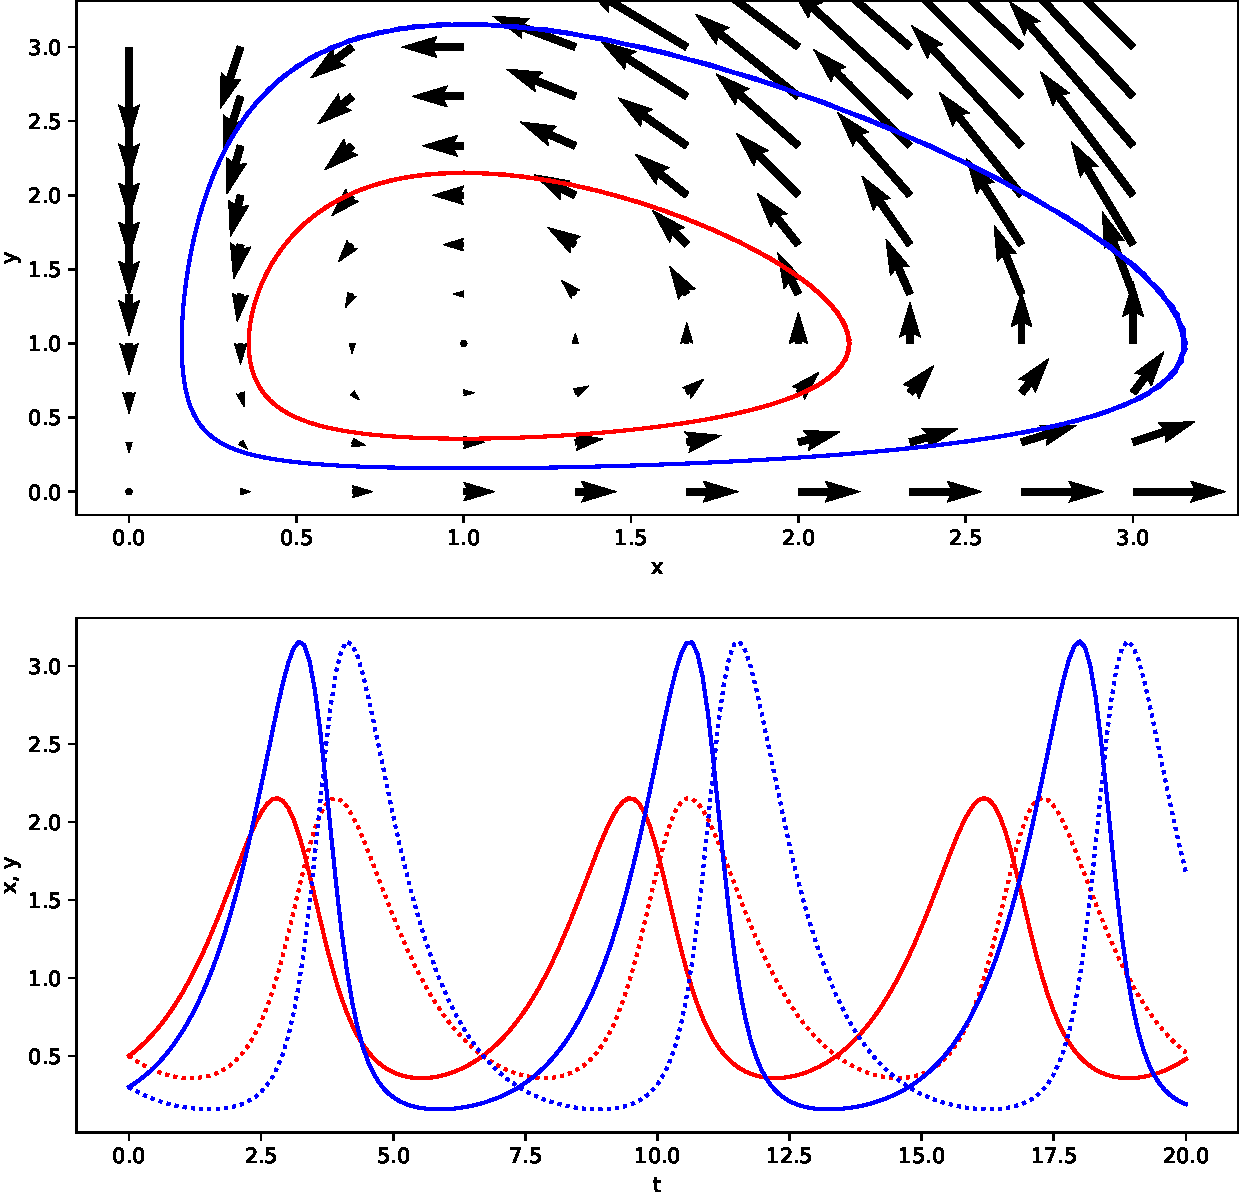
\includegraphics[width=0.75\textwidth]{LotkaVolterra.pdf}
	\caption{Phase portrait for the Lotka-Volterra model, showing oscillations around the critical point $(\frac{c}{\gamma}, \frac{a}{\alpha})$, and plot of the number of predator (dashed lines) and prey animals (solid lines) over time.}
	\label{fig:lotkavolterra}
\end{figure}

To finish on an interesting note, the qualitative behaviour of the model can be confirmed by data gathered on hare and lynx populations by the Hudson's Bay Company in Canada, shown in \Cref{fig:harelynx}. Specifically, the data consists of the number of furs from each animal bought each year, from which we make the (perhaps unrealistic) assumption that this is proportional to the actual populations of these animals.

\begin{figure}[!ht]
	\centering
	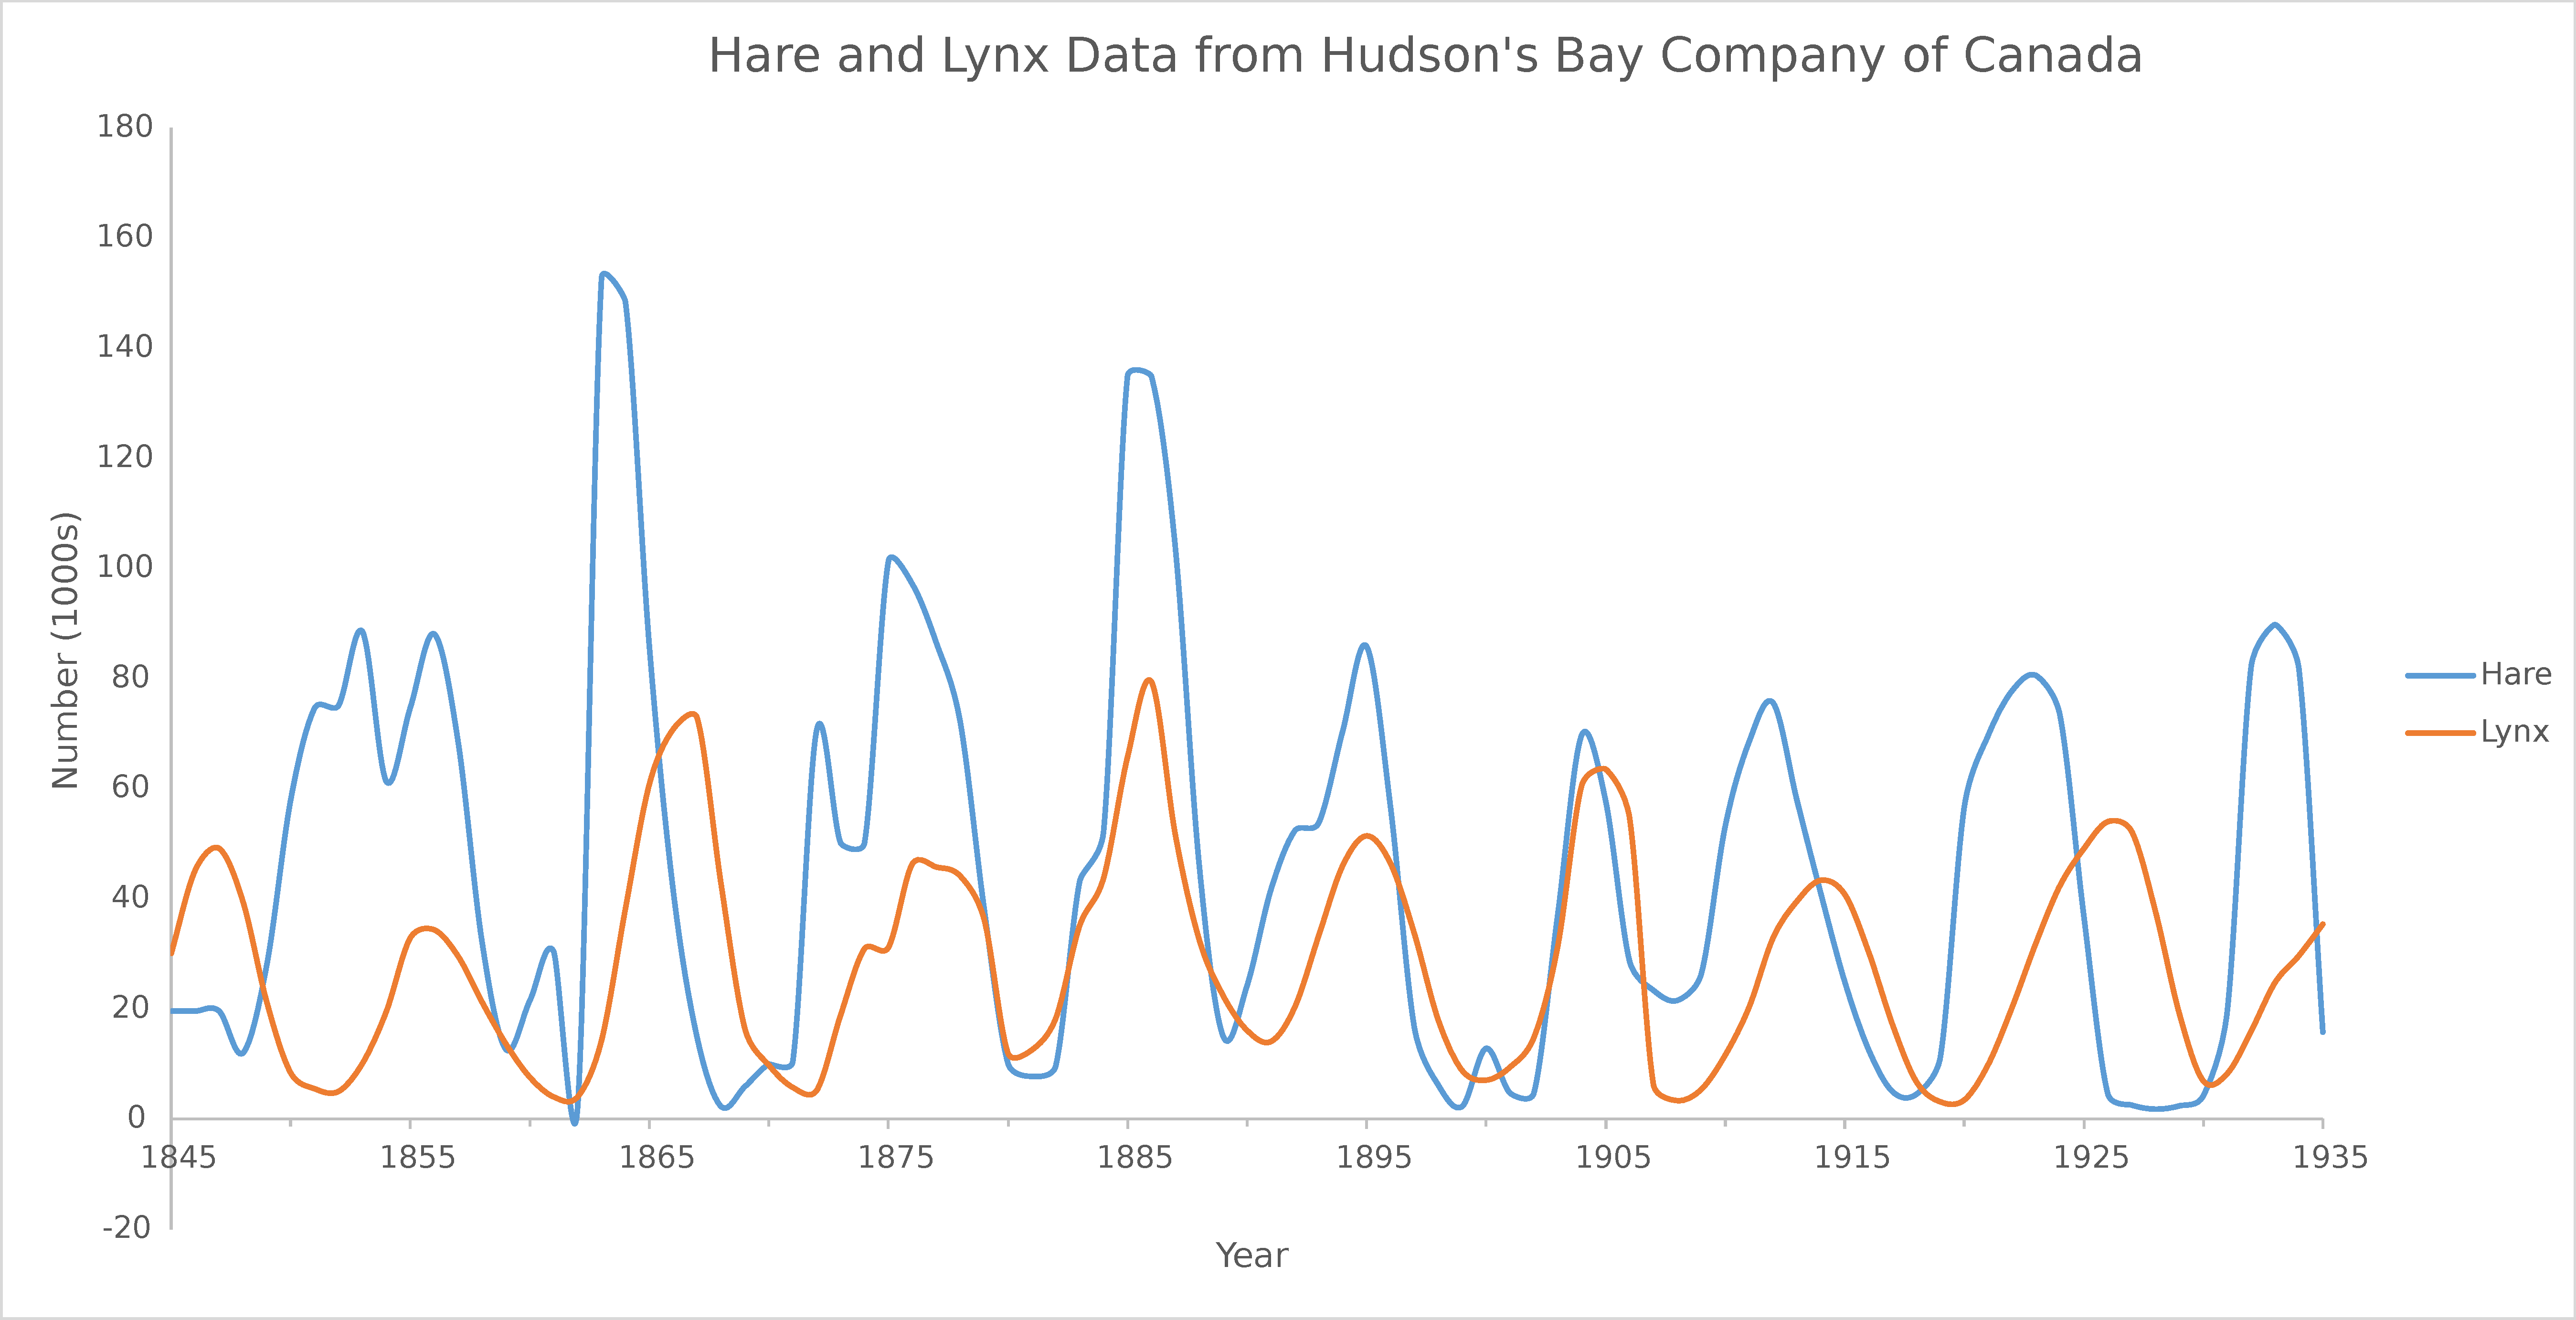
\includegraphics[width=\textwidth]{HareLynx.pdf}
	\caption{Hare and lynx data from Hudson's Bay Company (\href{https://www2.nau.edu/lrm22/lessons/predator_prey/predator_prey.html}{source}). Compare the periodic dynamics with the theoretic dynamics in \Cref{fig:lotkavolterra}.}
	\label{fig:harelynx}
\end{figure}

\subsection{Non-linear Methods}

We have seen how we can determine whether a critical point of a non-linear system is stable or unstable by using a linear approximation near the critical point. However, there are certain limitations to these methods, such as that the Jacobian may not give us any information about the system (e.g. when it is the zero matrix, as in \Cref{eg:lyapunov2}), or the critical point of the linearisation may be a centre, as was the case in the damped pendulum example (\Cref{eg:dampedpendulum2}) and the Lotka-Volterra Model of \Cref{sec:lotkavolterra}.

Therefore, we now develop methods that apply directly to analyse non-linear systems of ODEs.

\subsubsection{Lyapunov Methods}

For motivation, consider a particle on a one-dimensional landscape with variable height $h(x)$. Then the potential $V(x) = gh(x)$, where $g$ is the gravitational constant. Then by Newton's second law, $x'' = -V'(x)$.

We wish to transform this into a system of first-order ODEs, which we do via the usual method of defining a new variable $y=x'$, then $y' = x'' = -V'(x)$. So we have the following system:
\begin{align*}
	x' &= y \\
	y' &= -V'(x).
\end{align*}

From here, it is easy to see that the critical points occur when $y=0$ and $V'(x)=0$. In other words, the CP is $(x_*, 0)$ with $V'(x_*) = 0$. To see what information we can find about this critical point via the linearisation, we calculate the Jacobian:
\[
J = \mat{0 & 1 \\ -V''(x) & 0} \implies J\mid_{(x_*,0)} = \mat{0 & 1 \\ -V''(x_*) & 0}
\]
The characteristic equation of the Jacobian at the CP is
\[
r^2 + V''(x_*) = 0.
\]

Therefore, if $x_*$ is a minimum of $V(x)$ (so $V''(x)>0$),
\[
r = \pm i\sqrt{V''(x_*)},
\]
and the critical point of the linear system is a centre.

If $x_*$ is a maximum of $V(x)$ (so $V''(x)<0$),
\[
r = \pm \sqrt{-V''(x_*)},
\]
and the critical point is a saddle point, which is unstable.

Therefore, in the case that $x_*$ is a minimum of $V$, we cannot conclude about the (in)stability of the non-linear system based on the centre of the linear system. So what can we say about the system that is not limited to the behaviour of the linearised system near the critical points?

What we can do is define the following function $F$ which is time-invariant (the physics interpretation is that $F$ is the sum of kinetic and potential energy):
\[
F(x,y) = \frac{y^2}{2} + V(x).
\]
Then
\[
\frac{dF}{dt} = yy' + V'(x)x' = -yV'(x) + V'(x)y = 0.
\]
Therefore $F$ is constant along trajectories, which corresponds to our idea of it representing energy which is of course conserved (in an isolated system). Thus, we can also say that the trajectories are constant level curves of $F$.

Now, we define the function
\[
E(x,y) = F(x,y) - F(x_*,0) = \frac{y^2}{2} + V(x) - V(x_*).
\]

\begin{remark}
	$E$ is called a Lyapunov Function.
\end{remark}

Observe that $E(x_*, 0)=0$, $\frac{dE}{dt} = 0$, and that if $x_*$ is a minimum of $V$, $E(x,y) \geq 0$. On the other hand, if $x_*$ is a maximum, then $E$ is sign-indefinite, corresponding to a saddle point at the CP $(x_*,0)$.

Therefore in the case of the minimum, the level curves for $E$ are closed and bounded, giving a stable equilibrium that looks something like a centre.

To summarise, we found an implicit function $E$ with $\frac{dE}{dt} = 0$\footnote{Also works if $\frac{dE}{dt}<0$ or $\frac{dE}{dt}\leq0$} and $E \geq 0$, where the existence of this function implies that the critical point $(x_*,0)$ is stable. This idea is the foundation of Lyapunov's method.

Thus, we are now ready to state the formal definitions and methods relating to the Lyapunov Methods.

\begin{definition}
	$E(x,y)$ is positive definite if $E(x,y)>0$ for all $(x,y) \neq (0,0)$. Similarly, $E(x,y)$ is positive semi-definite if $E(x,y)\geq 0$ for all $(x,y) \neq (0,0)$.
\end{definition}

\begin{theorem}[Lyapunov Stability Theorem]\label{thrm:lyapunov1}
	If there exists a positive definite $E(x,y)$ such that $\frac{dE}{dt}$ is negative definite (semi-definite) on some domain $D$ containing the origin, then $\xta = (0,0)$ is asymptotically stable (stable).
\end{theorem}

\begin{theorem}[Lyapunov Instability Theorem]\label{thrm:lyapunov2}
	Suppose there exists $E(x,y)$ such that $E(0,0)=0$, and in every neighbourhood of the origin there is at least one point where $E$ is positive (negative). If there exists a domain $D$ containing the origin such that $\frac{dE}{dt}$ is positive definite (negative definite) on $D$, then the origin is an unstable critical point.
\end{theorem}

With the Lyapunov methods, we can see that, once we have a valid Lyapunov function $E$, it is not difficult to show that the conditions of Theorems \ref{thrm:lyapunov1} or \ref{thrm:lyapunov2} hold and therefore make conclusions on the stability/instability of the critical point. The difficult part of this process is finding the Lyapunov function $E$ in the first place.

To illustrate the application of these theorems, we consider the following examples.

\begin{eg}
	We have the system\footnote{Note that since this is a linear system, we can determine the stability of the critical points using the usual Jacobian-eigenvalue method. But that would ruin the fun of using our new-found theorems.}
	\begin{align*}
		x' &= -2x \\
		y' &= x-y.
	\end{align*}
	
	Fortunately, we have a flash of inspiration and decide to try
	\[
	E(x,y) = ax^2 + by^2, \quad a,b>0,
	\]
	where $E(x,y)>0$ for $(x,y)\neq(0,0)$.
	
	Using the chain rule,
	\begin{align*}
		\frac{d}{dt}E = 2axx' + 2byy' &= -4ax^2 + 2by(x-y) \\
		&= -2b\left(\frac{2a}{b}x^2 - xy + y^2\right) \\
		&= -2b\left(\frac{x}{2} - y\right)^2 \leq 0,
	\end{align*}
	where we pick $a$ and $b$ such that $\frac{2a}{b} = \frac14$ in order to factorise the second line.
	
	Therefore $E$ is positive definite and $E'$ is negative semi-definite, so by \Cref{thrm:lyapunov1}, the CP $(0,0)$ is stable.
\end{eg}

\begin{eg}\label{eg:lyapunov2}
	We have the system
	\begin{align*}
		x' &= -xy^2 \\
		y' &= 3x^2y
	\end{align*}
	It is easy to see that $(0,0)$ is a critical point of this system. However, the Jacobian at $(0,0)$ is the zero matrix, which tells us nothing about the linearised system. So non-linear methods are required.
	
	We try the function
	\[
	E(x,y) = 3x^2 + y^2 > 0 \text{ for } (x,y) \neq (0,0).
	\]
	So $E$ is positive definite. Furthermore,
	\[
	\frac{dE}{dt} = 6xx' + 2yy' = -6x^2y^2 + 6x^2y^2 = 0,
	\]
	so $\frac{dE}{dt}$ is negative semi-definite and by \Cref{thrm:lyapunov1}, $\xta = (0,0)$ is stable.
\end{eg}

\begin{eg}
	We have the system
	\begin{align*}
		x' &= x+3y \\
		y' &= 2x.
	\end{align*}
	Try $E(x,y) = xy + by^2 > 0$ for some $(x,y)$. Also, $E(0,0)=0$.	Then
	\begin{align*}
		\frac{dE}{dt} = x'y + xy' + 2byy' &= (x+3y)y + 2x^2 + 4bxy \\
		&= 3y^2 + 2x^2 + xy(1+4b).
	\end{align*}
	Set $b=-\frac14$ so that $1+4b=0$, then $\frac{dE}{dt}$ is positive definite, and by \Cref{thrm:lyapunov2}, the critical point $(0,0)$ is unstable.
\end{eg}

\subsubsection{Poincar\'{e}-Bendixson Theorem}

We'll now move on to discuss the existence of periodic trajectories. 

The Poincaré-Bendixson theorem tells us when such periodic orbits exist. But what are periodic trajectories? To put it quite simply: any closed trajectory is a periodic trajectory.

If a solution is closed, then it repeats itself with a period $T$ which implies that there exists $T>0$ such that $\vbx(t+T) = \xt$. 
We've already encountered periodic trajectories around critical points which are centres. In this case, we had a family of periodic trajectories in the form of a collection of elliptical trajectories, each closed and periodic. However, we can also encounter cases of isolated periodic trajectories.

\begin{eg}\label{eg:periodicsol}
	\begin{align*}
		x' &= y - x(x^2 + y^2 - a^2) \\
		y' &= -x -y(x^2 + y^2 - a^2).
	\end{align*}
	First, we find the critical point to be at the origin $(0,0)$ and the Jacobian at this critical point is given by: 
	\[
	J(0,0) = \mat{a^2 & 1 \\ -1 & a^2}.
	\]
	The eigenvalues associated with $J(0,0)$ are found as follows: 
	\[
	(a^2 - r)^2 + 1 = 0 \implies r = a^2 \pm i.
	\]
	Since the eigenvalues are a pair of complex conjugates which are not purely imaginary, we have that $(0,0)$ is an unstable focus as $a^2 > 0$ and $r_1$ and $r_2$ are complex conjugates. So the critical point $(0,0)$ is a spiral source.
	
	But, does this trajectory spiral away to infinity or does it change its behaviour at some point? Let's have a look at the polar co-ordinates to understand this better:
	
	Let $x = r \cos{\theta}, y = r \sin{\theta}$. Then,
	\begin{align}
		\label{eq3.14}
		x' &= r' \cos{\theta} - r \theta' \sin{\theta} = r \sin{\theta} - r \cos{\theta}(r^2 - a^2) \\
		\label{eq3.15}
		y' &= r' \sin{\theta} + r \theta' \cos{\theta} = - r \cos{\theta} - r \sin{\theta}(r^2 - a^2).
	\end{align}
	Multiplying \Cref{eq3.14} by $\cos{\theta}$ and \Cref{eq3.15} by $\sin{\theta}$ and adding them together, we get:
	\[
	r' = -r(r^2 - a^2).
	\]
	Multiplying \Cref{eq3.14} by $-\sin{\theta}$ and \Cref{eq3.15} by $\cos{\theta}$ and adding them together, we get:
	\[
	r\theta' = -r.
	\]
	So, we now have a system of ODEs of the form:
	\begin{align*}
		r' &= -r(r^2 - a^2) \\
		\theta' &= -1.
	\end{align*}
	So, all the trajectories are going to rotate at a constant angular velocity 
	\[
	\theta = \theta_0 - t.
	\]
	We can also look at the dynamics in the radial direction separately as $r$ does not depend on $\theta$.
	
	\underline{Radial dynamics}: Since $r' = -r(r^2 - a^2)$, at $r=a$, we have a periodic trajectory as $r' = 0$ and when $r<a$, $r'$ is positive so $r$ is going to increase towards $a$ and when $r>a$, $r'$ is negative so $r$ is going to decrease towards $a$. The trajectories are illustrated in \Cref{fig:periodicsol} in the $a=1$ case.
\end{eg}

\begin{figure}[!ht]
	\centering
	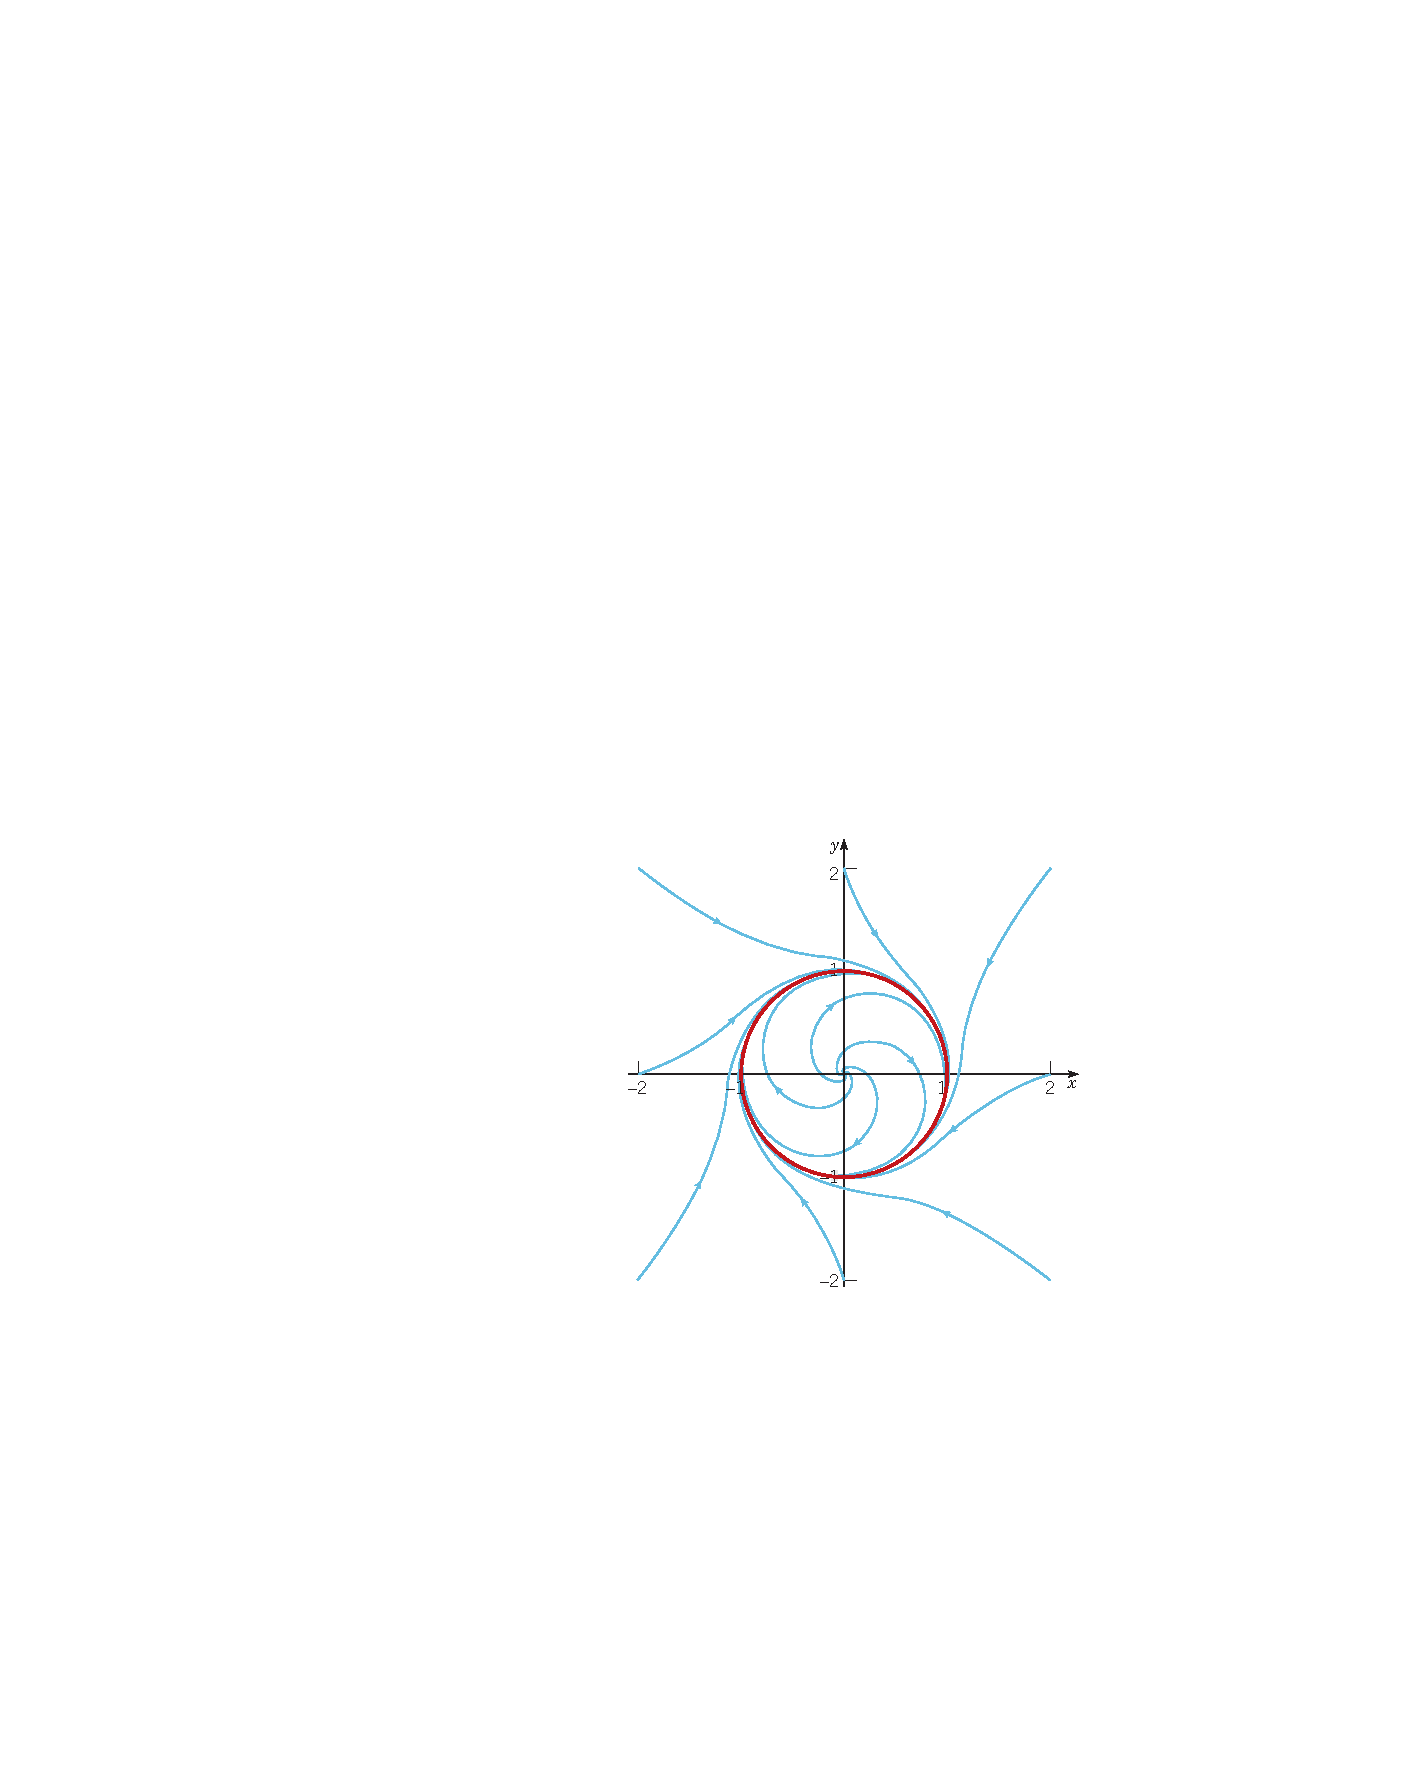
\includegraphics[width=0.5\textwidth]{PeriodicSol.pdf}
	\caption{Trajectories of the system in \Cref{eg:periodicsol} when $a=1$. Observe that all trajectories spiral toward the red circle with $r=1$ as $t \to \infty$ \cite[Figure 9.7.1]{boyce}.}
	\label{fig:periodicsol}
\end{figure}

The circle in the above example is an example of what is called a limit cycle.

\begin{definition}
	A limit cycle is a periodic solution such that at least one other non-closed trajectory tends to them as $t \to \infty$ or $t \to -\infty$ (or both).
\end{definition}

The limit cycle is (see \Cref{fig:limitcycles}): 
\begin{itemize}
	\item Asymptotically stable (or simply stable) if all nearby trajectories tend to it as $t \to \infty$.
	\item Asymptotically unstable (or simply unstable) if all trajectories go away from the limit cycle as $t \to \infty$.
	\item Semi-stable (or half-stable) when trajectories tend to the limit cycle from one side but move away from the limit cycle from the other side.
\end{itemize}

The example in \Cref{eg:periodicsol} was asymptotically unstable.

\begin{figure}[!ht]
	\centering
	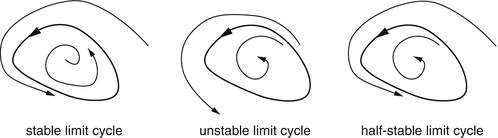
\includegraphics[width=0.9\textwidth]{LimitCycles.png}
	\caption{Graphical representation for each of the three types of limit cycle \cite{limitcycles}.}
	\label{fig:limitcycles}
\end{figure}

\subsubsection*{Existence of limit cycles and periodic trajectories}

Consider a set of autonomous functions $F$ and $G$ which are continuously differentiable on a domain $D$.

\begin{theorem}\label{thrm:periodictraj1}
	A closed trajectory must enclose at least one critical point. If this critical point is unique, then it cannot be a saddle point.
\end{theorem}

\begin{proof}
	While the mathematical proof will not be discussed here, the topological reasoning might be helpful. 
	The uniqueness of the critical point implying that the critical point cannot be a saddle point holds because if we do imagine a saddle point surrounded by a periodic trajectory, it could look something like \Cref{fig:cpnosaddle} where $A$ is the saddle point but $B$ and $C$ could be other critical points which then contradicts that $A$ is the only critical point.
\end{proof}

\begin{figure}[!ht]
	\centering
	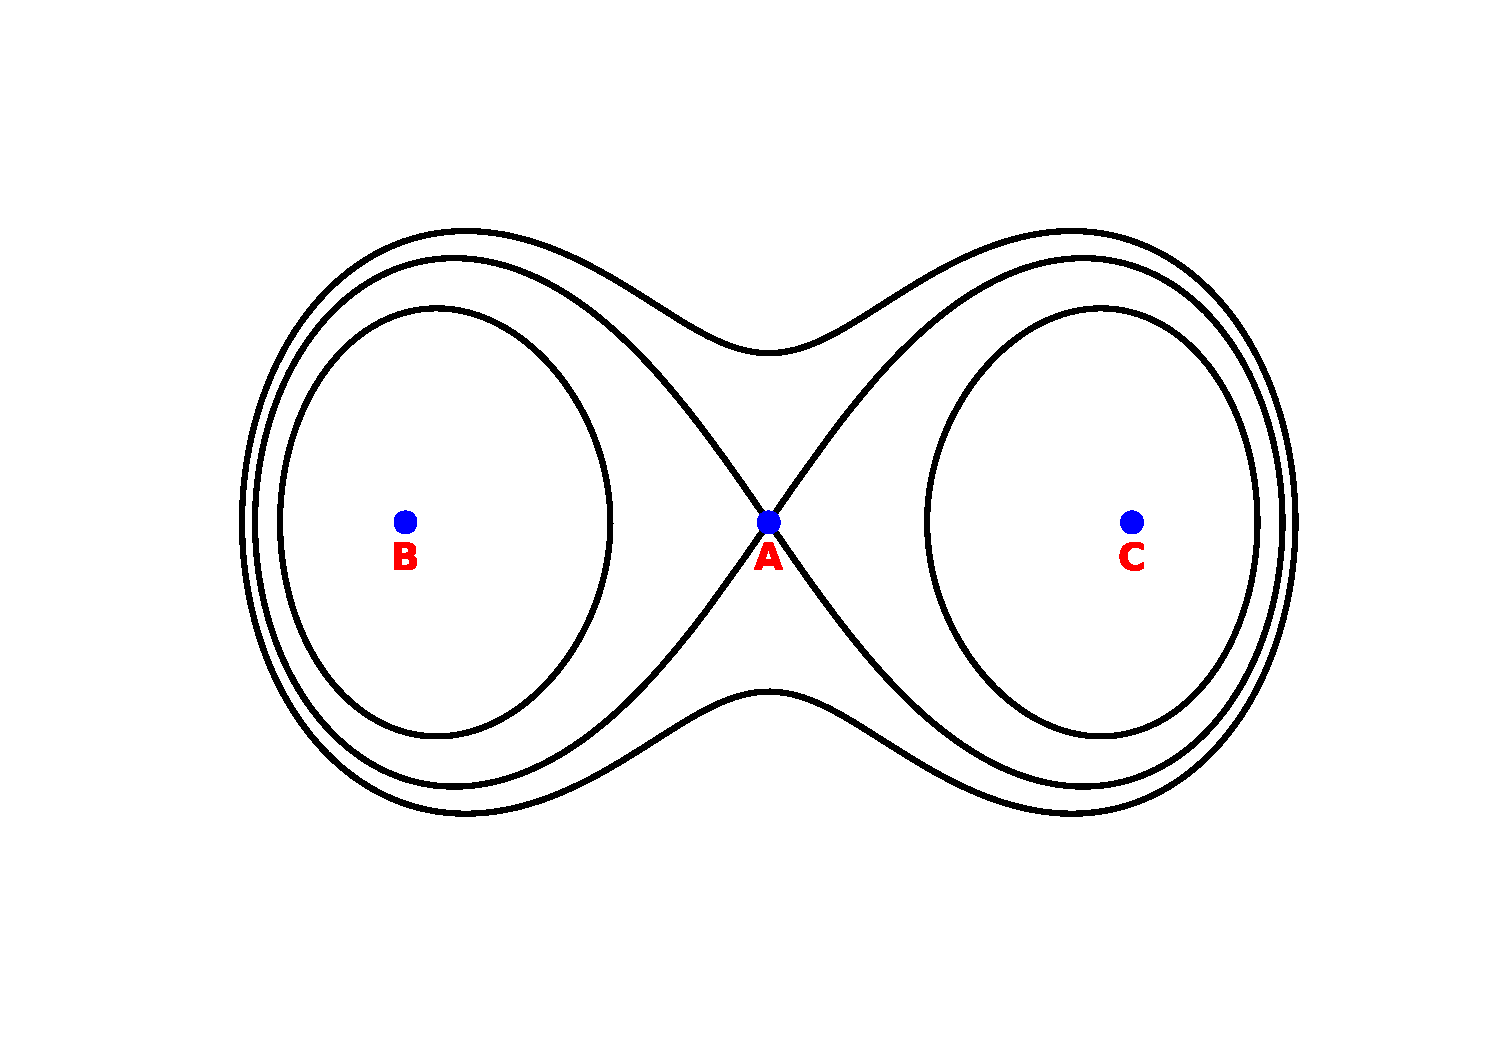
\includegraphics[width=0.55\textwidth]{CPNoSaddle.pdf}
	\caption{In this example, the trajectories are \href{https://mathworld.wolfram.com/CassiniOvals.html}{Cassini ovals}.}
	\label{fig:cpnosaddle}
\end{figure}

The negative version of this theorem is more useful:

\begin{theorem}\label{thrm:periodictraj2}
	Assume $\p_x F(x,y) + \p_y G(x,y) \neq 0$ in a simply connected domain $D$, then there are no periodic trajectories in $D$.
\end{theorem}

\begin{proof}
	A simply connected two-dimensional domain is one with no holes. If you've not already noticed, $\p_x F(x,y) + \p_y G(x,y)$ is the divergence of (F,G). Divergence is the measure of contraction or expansion of an area under the vector field, as in \Cref{fig:divergence}.
	
	\begin{figure}[!ht]
		\centering
		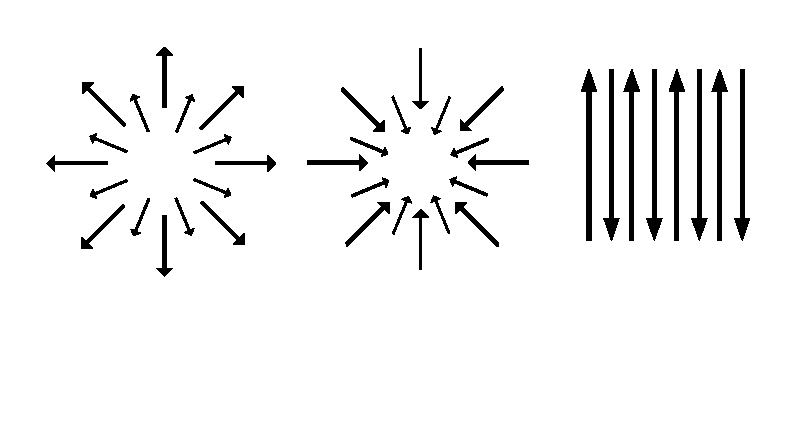
\includegraphics[width=0.8\textwidth]{Divergence.pdf}
		\caption{(Left to right) Positive, negative, and zero divergence of a vector field at a point (source: \href{https://commons.wikimedia.org/wiki/File:Divergence_(captions).svg}{Wikimedia}).}
		\label{fig:divergence}
	\end{figure}
	
	In fact, by Green's theorem,
	\[
	\frac{dA}{dt} = (\p_x F + \p_y G)A.
	\]
	In other words, the rate of change of an area is given by the divergence of the vector field times the area.
	
	Now, if you have a closed trajectory, the area inside is going to evolve into itself. So, the rate of change of the interior of this trajectory should be zero. Thus, if the area is increasing (or decreasing) because $(\p_x F + \p_y G) \neq 0$, then the closed trajectory would expand (or contract) and so, it cannot be invariant under the ODEs.
\end{proof}

\begin{remark}
	Note that the above two theorems help to rule out trajectories that are not periodic rather than prove that they are periodic.
\end{remark}

\begin{eg}
	We work with the same system as in \Cref{eg:periodicsol}:
	\begin{align*}
		x' &= y - x(x^2 + y^2 - a^2) = F(x,y) \\
		y' &= -x - y(x^2 + y^2 - a^2) = G(x,y).
	\end{align*}
	Then, 
	\begin{align*}
		\p_x F + \p_y G &= -(x^2 + y^2 - a^2) - 2x^2 - (x^2 + y^2 - a^2) - 2y^2 \\
		&= -4x^2 - 4y^2 + 2a^2 \\
		&= -4r^2 + 2a^2.
	\end{align*}
	
	So for $r < \frac{a}{\sqrt{2}}$, $\p_x F + \p_y G > 0$. Therefore, there is no periodic trajectory in this region by \Cref{thrm:periodictraj2}.
	
	We already know from the earlier example that $r$ has no periodic trajectory when $0<r<a$, so this theorem is not the most optimum one we can use, but it still offers some idea of a region in the phase plane that does not have a periodic trajectory. 
\end{eg}

\begin{theorem}[Poincar\'{e}-Bendixson theorem]
	Consider $D_1 \subset D$. Let the functions $F$ and $G$ have continuous first partial derivatives in a domain $D$ of the $xy$-plane and $R := D_1 \cup \p D_1$ (where $\p D_1$ is the boundary of $D_1$). Suppose there are no critical points in $R$ and there exists a trajectory $(x(t),y(t)) \in R$ for all $t$. Then either $(x(t),y(t))$ is periodic or it tends to a periodic trajectory.
\end{theorem}

\begin{remark}
	From \Cref{thrm:periodictraj1}, when we have a region enclosed by a periodic trajectory, then there exists a critical point somewhere in the region. So, to make the Poincaré-Bendixson theorem valid, we have to show that there is no critical point, yet there exists a periodic trajectory. So, $R$ should not be simply connected and must contain a hole at the critical point so that both \Cref{thrm:periodictraj1} and the Poincaré-Bendixson theorem hold.
\end{remark}

\begin{remark}
	The key to using the theorem is not to find a trajectory that does not leave the domain, but rather to find a trapping region $R$ such that once a trajectory enters the region, it never leaves.
	
	So, to prove that $R$ is a trapping region, we show that the vector field is pointing toward the interior of the domain $R$ everywhere, e.g. as in \Cref{fig:trappingregion}.
\end{remark}

\begin{figure}[!ht]
	\centering
	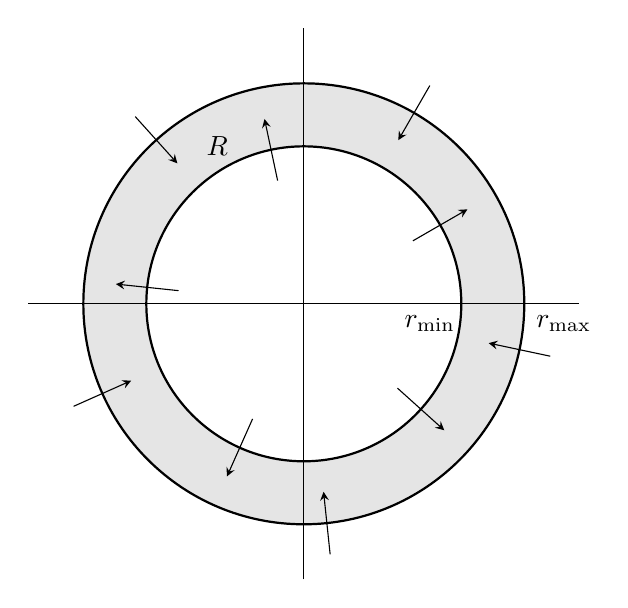
\begin{tikzpicture}
		\filldraw[color=black, fill=gray!20, thick] (0,0) circle (2.8);
		\filldraw[color=black, fill=white, thick] (0,0) circle (2);
		\draw (-3.5,0) -- (3.5,0);
		\draw (0,-3.5) -- (0,3.5);
		\node at (1.6,-0.25) {$r_{\text{min}}$};
		\node at (3.3,-0.25) {$r_{\text{max}}$};
		\node at (-1.1, 2) {$R$};
		\foreach \x in {0,...,4}{
			\draw[-stealth] (30+72*\x:1.6) -- (30+72*\x:2.4);
			\draw[-stealth] (60+72*\x:3.2) -- (60+72*\x:2.4);
		}
	\end{tikzpicture}
	\caption{An example of a trapping region $R$, where the vector field always points towards the interior of $R$.}
	\label{fig:trappingregion}
\end{figure}

\begin{eg}
	Returning to the system from \Cref{eg:periodicsol} where we found
	\[
	r' = -r(r^2 - a^2),
	\]
	let $R = {\frac{a}{2}<r<2a}$. Then, $r' > 0$ for $r = \frac{a}{2}$ and $r'<0$ for $r = 2a$.
	
	Thus, $R$ is a trapping region (essentially looking like \Cref{fig:trappingregion}). There are no critical points in this region as $(0,0)$ is the only critical point for the system which is not included in the trapping region $R$. So by the Poincaré-Bendixson theorem, there exists a periodic trajectory in $R$.
\end{eg}

\begin{eg}
	Consider the system
	\begin{align*}
		x' &= y \\
		y' &= -x + y(1-3x^2-2y^2).
	\end{align*}
	To find whether a limit cycle exists in this system, let $r^2 = x^2 + y^2$. Then,
	\begin{align*}
		rr' & = xx' + yy' \\
		& = xy - xy + y^2(1-3x^2-2y^2) \\
		& = y^2(1-3x^2-2y^2).
	\end{align*}
	So, 
	\[
	rr' \geq y^2(1 - 3x^2 - 3y^2) \geq y^2(1-3r^2) \geq 0 
	\] if $r \leq \frac{1}{\sqrt{3}}$
	and
	\[
	rr' \leq y^2(1 - 2x^2 - 2y^2) \leq y^2(1-2r^2) \leq 0 
	\] if $r \geq \frac{1}{\sqrt{2}}$.
	
	Thus, a trapping region is given by $R := \{r: \frac{1}{\sqrt{3}} \leq r \leq \frac{1}{\sqrt{2}}\}$\footnote{Since at the borders $r=\frac{1}{\sqrt{3}}$ and $r=\frac{1}{\sqrt{2}}$, the trajectories point towards the interior of $R$ (or, at the very least, do not point outwards).} which does not include a critical point and by the Poincaré-Bendixson theorem, there exists a periodic trajectory in the system of ODEs.
\end{eg}
\section{Fourier Series}

So far we've considered initial value problems while solving ODEs. While looking at second-order ODEs, we are given the value of the function and its derivative at a given time. In boundary value problems, we are given the value of the function at two different points (i.e. 2 points on the boundary of the domain).

Boundary eigenvalue problems are a generalisation to functions of eigenvalue problems for matrices. This yields eigenvectors that form a basis in a function space. 

\subsection{Boundary Value \& Eigenvalue Problems}\label{sec:boundaryvalprob}

\begin{eg}\label{eg:bvpmotiv}
	We consider the following boundary value problem involving a second-order ODE:
	\[
	y'' + y = 0 \qquad y'(0)=1, \,\, y(\pi) = a
	\]
	
	The solution is given by: 
	\[
	y = A \cos{x} + B \sin{x}
	\]
	Imposing the boundary conditions:
	\begin{align*}
		y(0) &= A = 1 \\
		y(\pi) &= -A = a
	\end{align*}
	
	If $a \neq -1$, then there is no solution to the boundary value problem.
	
	If $a = -1$, there are infinitely many solutions to the boundary value problem as $y(x) = \cos{x} + B\sin{x}$ where $B \in \R$. 
\end{eg}
	
This illustrates one way in which boundary value problems differ from initial value problems: while the IVP
\[
	y'' + p(t)y' + q(t)y = g(t), \quad y(t_0) = \alpha, y'(t_0) = \beta
\]
is guaranteed to have a unique solution on an open interval $I$ provided that $p$, $q$, and $g$ are continuous on $I$, the boundary value problem
\[
	y'' + p(x)y' + q(x)y = g(x), \quad y(x_1) = \alpha, y(x_2) = \beta
\]
could have a unique solution, many solutions, or no solution, depending on the boundary conditions.
	
The above \Cref{eg:bvpmotiv} having infinitely many solutions in the case of $a = -1$ is similar to the case of $A\vbx = \bm{b}$ where $A$ is a singular matrix. There are no solutions to this system unless $\bm{b}$ is orthogonal to any vector in the kernel of $A^T$. So, $\bm{b} \cdot \bm{y} = 0$ for all $\bm{y} \in \R^n$ such that $A^T \bm{y} = 0$.

Recall the matrix eigenvalue problem: 
\begin{equation}\label{eq4.1}
	A \xib_i = \lambda_i \xib_i
\end{equation}
The eigenvalue problem helps us find non-trivial solutions to \Cref{eq4.1}, which will exist only if $\lambda_i$ are eigenvalues of $A$. In addition, if $A$ is diagonalisable, then $\xib_i$ form a basis of $\R^n$ and $\xt = \sum_{i=1}^n c_i \xib_i$.

If $A^T = A$, the matrix is symmetric and the eigenvectors are orthogonal so $\xib_i \cdot \xib_j = 0$ for $i \neq j$. So, we have that
\begin{align*}
	\vbx &= \sum_{i=1}^n c_i \xib_i \\
	\xib_j \cdot \vbx &= \sum_{i=1}^n c_i \xib_i \cdot \xib_j
\end{align*}
but since $\xib_i \cdot \xib_j = 0$ for $i \neq j$, 
\begin{align*}
	\xib_j \cdot \vbx = c_j \Vert \xib_j \Vert^2
\end{align*}
So, in this case, the fact that the basis is orthogonal makes finding the coefficients $c_i$ easier when we want to represent some vector using this basis.


We now look at an equivalent of the eigenvalue problem $A \xib = \lambda \xib$. We can consider $A$ to be a linear map and we know that linear maps can act on functions. An operator $Ly(x)$ is linear if and only if $L(ay_1(x) + by_2(x)) = aLy_1(x) + bLy_2(x)$

\begin{eg}\label{eg:linearmap}
	The following are linear operators:
	\begin{itemize}
		\item $L = \frac{d^2}{dx^2}$ since $\frac{d^2}{dx^2}(ay_1 + by_2) = a \frac{d^2}{dx^2}y_1 + b \frac{d^2}{dx^2}y_2$.
		\item $L = p(x)\frac{d^2}{dx^2} + q(x)\frac{d^2}{dx^2}$.
	\end{itemize}
\end{eg}

So the generalisation of eigenvalue problems for functions would be $Ly(x) = \lambda y(x)$.

\begin{eg}\label{eg:eigenvalprob}
	\[
	y'' = \lambda y \qquad y(0) = y(L) = 0
	\]
	We look at the following 3 cases:
	\begin{itemize}
		\item Case 1: $\lambda = \mu^2 > 0$.\\
		The ODE is given by: $y'' - \mu^2 y = 0$.\\
		In this case, the solution is given by:\footnote{Since $e^{\mu x}$ and $e^{-\mu x}$ are fundamental solutions, and $\cosh{\mu x} = \frac12(e^{\mu x} + e^{-\mu x})$ and $\sinh{\mu x} = \frac12(e^{\mu x} - e^{-\mu x})$ i.e. they are linear combinations of $e^{\mu x}$ and $e^{-\mu x}$.}
		\[
		y(x) = A \cosh{\mu x} + B \sinh{\mu x}.
		\]
		Using the boundary values:
		\begin{align*}
			y(0) &= A = 0 \\
			y(L) &= B \sinh{\mu L} = 0 \implies B=0
		\end{align*}
		So there is no non-trivial solution in this case.
		
		\item Case 2: $\lambda = 0$.\\
		The ODE is given by: $y''= 0$.\\
		In this case, the solution is given by:
		\[
		y(x) = Ax + B.
		\]
		Using the boundary values:
		\begin{align*}
			y(0) &= B = 0 \\
			y(L) &= AL = 0 \implies A = 0
		\end{align*}
		So there is no non-trivial solution in this case.
		
		\item Case 3: $\lambda = -\mu^2 < 0$.\\
		The ODE is given by: $y'' + \mu^2 y = 0$.\\
		In this case, the solution is given by:
		\[
		y(x) = A \cos{\mu x} + B \sin{\mu x}.
		\]
		Using the boundary values:
		\begin{align*}
			y(0) &= A = 0 \\
			y(L) &= B \sin{\mu L} = 0
		\end{align*}
		In this case, however, $B \neq 0$ if $\mu L = n \pi$ where $n \in \Z$. So, we have non-trivial solutions $\lambda = -\mu^2$ where $\mu = \frac{n \pi}{L}$.
	\end{itemize}
	Thus, the eigenvalues are given by: $\lambda_n = -\frac{n^2\pi^2}{L^2}$, where $n = 1, 2, \dots$, and the eigenfunctions are given by: $y_n(x) = \sin\left(\frac{n\pi x}{L}\right)$.
	
	So, we have a set of eigenvalues and eigenfunctions for the ODE.
\end{eg}

\begin{eg}\label{eg:bvpmotiv2}
	\[
	y'' = \lambda y \qquad y(x+2L) = y(x)
	\]
	Here, we see a periodic function with period $2L$. Equivalently,
	\begin{align*}
		y(-L) &= y(L) \\
		y'(-L) &= y'(L)
	\end{align*}
	\begin{itemize}
		\item Case 1: $\lambda = \mu^2 > 0$.\\
		The ODE is given by: $y'' - \mu^2 y = 0$.\\
		In this case, the solution is given by:
		\[
		y(x) = A \cosh{\mu x} + B \sinh{\mu x},
		\]
		Using the boundary conditions:
		\begin{align*}
			y(-L) &= A \cosh{\mu L} - B \sinh{\mu L} \\
			y(L) &= A \cosh{\mu L} + B \sinh{\mu L} \\
			y(-L) &= y(L) \implies B = 0 \\
			y'(-L) &= y'(L) \implies A = 0 
		\end{align*}
		So, there is no non-trivial solution in this case.
		
		\item Case 2: $\lambda = 0$.\\
		The ODE is given by: $y''= 0$.\\
		In this case, the solution is given by:
		\[
		y(x) = Ax + B.
		\]
		Using the boundary conditions:
		\begin{align*}
			y(-L) &= -AL + B\\
			y(L) &= AL + B \\
			y(-L) &= y(L) \implies A = 0 \\
			y'(-L) &= y(L) \implies B \text{ is a free parameter.}
		\end{align*}
		So, the only non-trivial function in this case is the constant function $y(x)=B$.
		
		\item Case 3: $\lambda = -\mu^2 < 0$.\\
		The ODE is given by: $y'' + \mu^2 y = 0$.\\
		In this case, the solution is given by:
		\[
		y(x) = A \cos{\mu x} + B \sin{\mu x}
		\]
		Using the boundary conditions:
		\begin{align*}
			y(-L) & = A \cos{\mu L} - B \sin{\mu L} \\
			y(L) & = A \cos{\mu L} + B \sin{\mu L}
		\end{align*}
		\[
		y(-L) = y(L) \implies B \sin{\mu L} = 0 \implies \mu L = n \pi
		\]
		\begin{align*}
			y'(-L) & = \mu A \sin{\mu L} + \mu B \cos{\mu L} \\
			y'(L) & = -\mu A \sin{\mu L} + \mu B \cos{\mu L}
		\end{align*}
		\[
		y'(-L) = y'(L) \implies A \sin{\mu L} = 0 \implies \mu L = n \pi
		\]
		So, we have non-trivial solutions $\lambda = -\mu^2$ where $\mu = \frac{n \pi}{L}$.
	\end{itemize}
	Thus, the eigenvalues are given by: $\lambda_n = -\frac{n^2\pi^2}{L^2}$, where $n =0, 1, 2, \dots$, and the eigenfunctions are given by: $1, \cos\left(\frac{n\pi x}{L}\right), \sin\left(\frac{n\pi x}{L}\right)$.
	
	So, we have found a set of eigenvalues and eigenfunctions for the ODE.
\end{eg}

\subsection{Euler-Fourier Formulas}

\begin{definition}
	A function $f(x)$ is periodic if $f(x+T) = f(x) \,\, \forall x$. We say its	period is $T$. The smallest possible $T$ is the \textbf{fundamental period}.
\end{definition}

\begin{remark}
	Note that the convention used here is that that the period is $2L$, as is also used by Boyce. Other texts may differ, however.
\end{remark}

The Fourier series is a series that expresses a periodic function as an infinite sum of sines and cosines.
\begin{definition}\label{def:fourier}
	The Fourier series for a function $f(x)$ with period $2L$ is given by: 
	\[
		f(x) = \frac{a_0}{2} + \sum_{n=1}^{\infty} \left(a_n \cos{\left(\frac{n\pi x}{L}\right)} + b_n \sin{\left(\frac{n\pi x}{L}\right)}\right)
	\]
	where $a_0, a_n, b_n$ are coefficients that can be calculated using the Euler-Fourier formulas. The coefficients are real if $f(x)$ is real.
\end{definition}

Considering periodic functions $f(x+2L) = f(x)$, we looked at the eigenvalue problem: $y'' = \lambda y$ in \Cref{eg:bvpmotiv2}. The eigenvalues were found to be
\[
\lambda_n = -\frac{n^2 \pi^2}{L^2} 
\]
and corresponding eigenfunctions were 
\begin{align*}
	n &= 0, \quad y_0 = 1 \\
	n &\neq 0, \quad y_n = \cos{\left(\frac{n \pi x}{L}\right)}, \sin{\left(\frac{n \pi x}{L}\right)}
\end{align*}
So the basis is given by: $\left\{1, \cos{(\frac{n \pi x}{L})}, \sin{(\frac{n \pi x}{L})}\right\}$.

It is useful to have that the eigenfunctions are orthogonal. In this case, consider the inner product (the dot product) given by:
\begin{equation}\label{eq:innerprod}
	(u(x), v(x)) = \int_{-L}^L u(x) v(x) dx
\end{equation}
Then , the functions $\{1, \cos{(\frac{n \pi x}{L})}, \sin{(\frac{n \pi x}{L})}\}$ are orthogonal for this inner product.

The proof is as follows: Denote $C_n(x) = \cos{(\frac{n \pi x}{L})}$, $S_n(x) = \sin{(\frac{n \pi x}{L})}$, and $C_0(x)=1$. Now, consider
\begin{align*}
	\left(S_n(x), S_m(x)\right) &= \int_{-L}^L \sin{\left(\frac{n \pi x}{L}\right)} \sin{\left(\frac{m \pi x}{L}\right)} \,dx \\
	&= \frac{1}{2} \int_{-L}^L \cos{\left(\frac{(n-m) \pi x}{L}\right)} - \cos{\left(\frac{(n+m) \pi x}{L}\right)} \,dx
\end{align*}
If $n \neq m$, then
\[
\left(S_n(x), S_m(x)\right) = \frac{L}{2} \left(  \begin{bmatrix}\dfrac{\sin{\left(\frac{(n-m) \pi x}{L} \right)} }{(n-m) \pi} \end{bmatrix}_{-L}^L - \ \begin{bmatrix} \dfrac{\sin{\left(\frac{(n+m) \pi x}{L} \right)} }{(n+m) \pi} \end{bmatrix}_{-L}^L \right) = 0,
\]
since at every point we are evaluating sin at some integer multiple of $\pi$, which is zero.

If $n = m$, then
\begin{align*}
	\left(S_n(x), S_n(x)\right) & = \int^L_{-L} \sin^2{\left(\frac{n \pi x}{L}\right)} dx = \frac{1}{2} \int^L_{-L} 1 - \cos{\left(\frac{n \pi x}{L}\right)} dx \\
	&= \frac{1}{2}\left( 2L - L \left[ \sin{\left(\frac{2 \pi x}{L} \right)} \right]_{-L}^L \right) = L.
\end{align*}
From the above, we see that the sin functions have orthogonality as:
\[
(S_n, S_m) = L \delta_{mn} \quad \text{where } \delta_{mn} = \begin{cases}0 & \text{if } m \neq n \\ 1 & \text{if } m = n
\end{cases}
\]
where $\delta_{mn}$ is the Kronecker delta.

Similarly, we find that:
\[
(C_n, C_m) = L \delta_{mn} \quad \text{where } \delta_{mn} = \begin{cases}0 & \text{if } m \neq n \\ 1 & \text{if } m = n
\end{cases}
\]
And finally,
\begin{align*}
	(S_n, C_m) &= 0 \\
	(C_0, C_0) &= 2L
\end{align*}
The calculations of these two are left as an exercise to the reader.

With this information in hand, we are now ready to find the Fourier series for a $2L$ periodic function $f$. Reminder from \Cref{def:fourier} that the Fourier series is
\[
f(x) = \frac{a_0}{2} + \sum_{n=1}^{\infty} \left(a_n \cos{\left(\frac{n\pi x}{L}\right)} + b_n \sin{\left(\frac{n\pi x}{L}\right)}\right)
\]
where $a_n, b_n$ are Fourier coefficients. The coefficient of function $C_0 = 1$ is $\frac{a_0}{2}$.

To calculate $a_n, b_n$, we project $f(x)$ on the basis as follows (for $n \neq 0$): 
\begin{align*}
	(f(x), C_n) & = \left( \frac{a_0}{2} + \sum_{m=1}^{\infty} \left(a_m C_m(x) + b_m S_m(x) \right), C_n \right) \\
	& = \frac{a_0}{2}\cancelto{0}{(1,C_n)} + \sum_{m=1}^{\infty} a_m\cancelto{L\delta_{mn}}{(C_m, C_n)} + \sum_{m=1}^{\infty} b_m\cancelto{0}{(S_m, C_n)} \\
	&= a_n L.
\end{align*}

Therefore,
\begin{align*}
	a_n = \frac{1}{L} (f(x), C_n(x)) = \frac{1}{L} \int_{-L}^L f(x) \cos{\left(\frac{n \pi x}{L}\right)} dx
\end{align*}\

Similarly, $b_n$ is calculated by projecting $f$ on $\sin{\left( \frac{n \pi x}{L} \right)}$ and using orthogonality we get:
\[
b_n = \frac{1}{L} \int_{-L}^L f(x) \sin{\left( \frac{n \pi x}{L} \right)} dx
\]

Thus, we have the Euler-Fourier formulas:
\begin{align}
	\label{eq:eulerfourier1}
	a_n &= \frac{1}{L} \int_{-L}^L f(x) \cos{\left( \frac{n \pi x}{L} \right)} dx \\
	\label{eq:eulerfourier2}
	b_n &= \frac{1}{L} \int_{-L}^L f(x) \sin{\left( \frac{n \pi x}{L} \right)} dx \\
	\label{eq:eulerfourier3}
	a_0 &= \frac{1}{L} \int_{-L}^L f(x) dx
\end{align}

\begin{eg}\label{eg:fourier1}
	We calculate the Fourier series for the function 
	\( f(x) = \begin{cases} 
		0 & \text{if } -3<x<-1 \\
		1 & \text{if } -1<x<1 \\
		0 & \text{if } 1<x<3 \\
	\end{cases}\)
	with $f(x+6) = f(x)$. Here, $L=3$ since the convention of the period is $2L$. 
	
	In calculating the Fourier coefficients using the Euler-Fourier formulas in \Cref{eq:eulerfourier1,eq:eulerfourier2,eq:eulerfourier3}, we will make use of the fact $f(x)=0$ everywhere except $-1<x<1$. First, we find $a_0$,
	\begin{align*}
		a_0 &= \frac{1}{L} \int_{-L}^{L} f(x)dx = \frac{1}{3} \int_{-1}^{1} f(x)dx \\
		&= \frac{1}{3} \big[1\big]^1_{-1} = \frac{2}{3}.
	\end{align*}
	Now, we find $a_n$ for $n\neq 0$,
	\begin{align*}
		a_n &= \frac{1}{L} \int_{-L}^L f(x) \cos{\left( \frac{n \pi x}{L} \right)} dx = \frac{1}{3} \int_{-1}^1 \cos{\left( \frac{n \pi x}{3} \right)} dx \\
		&= \frac{1}{3} \cdot 3 \begin{bmatrix} \dfrac{\sin{\left( \frac{n \pi x}{3} \right)}}{n \pi} \end{bmatrix}^1_{-1} = \frac{2}{n \pi} \sin{\left( \frac{n \pi}{3} \right)}.
	\end{align*}
	Finally, we calculate the coefficients $b_n$,
	\begin{align*}
		b_n &= \frac{1}{3} \int_{-1}^1 f(x) \sin{\left( \frac{n \pi x}{3} \right)} dx = \frac{1}{3} \int_{-1}^1 \sin{\left( \frac{n \pi x}{3} \right)} dx = 0
	\end{align*}
	since $\sin\left(\frac{n \pi x}{3}\right)$ is an odd function.
	
	Thus, in sum, the Fourier coefficients are given by
	\[
	a_0 = \frac23, \quad a_n = \frac{2}{n \pi} \sin{\left( \frac{n \pi}{3} \right)}, \quad b_n = 0,
	\]
	and we have the Fourier series
	\[
	f(x) = \frac{1}{3} + \sum_{n=1}^{\infty} \left( \frac{2}{n \pi} \sin{\left( \frac{n \pi}{3} \right)} \cos{\left( \frac{n \pi x}{3} \right)} \right).
	\]
\end{eg}

When working with Fourier series such as the one in this example in practice, it is clearly not possible to use the infinite sum. Therefore, we must truncate the Fourier series by taking only the first $N$ terms. As an example, the Fourier series for the function in \Cref{eg:fourier1} with $N=100$ is given in \Cref{fig:fouriereg100}.

\begin{figure}[!ht]
	\centering
	\includegraphics[width=0.7\textwidth]{FourierSeries/EX1.100.pdf}
	\caption{Fourier series for $f$ in \Cref{eg:fourier1} with first 100 terms.}
	\label{fig:fouriereg100}
\end{figure}

It should not be at all surprising that the more terms we take, the better the approximation by Fourier series. See for example \Cref{fig:fourieregsub}, where the truncated Fourier series approximations for $N=2$ and $N=6$ do not resemble the function very well at all.

\begin{figure}[!ht]
	\centering
	\begin{subfigure}[b]{0.49\textwidth}
		\centering
		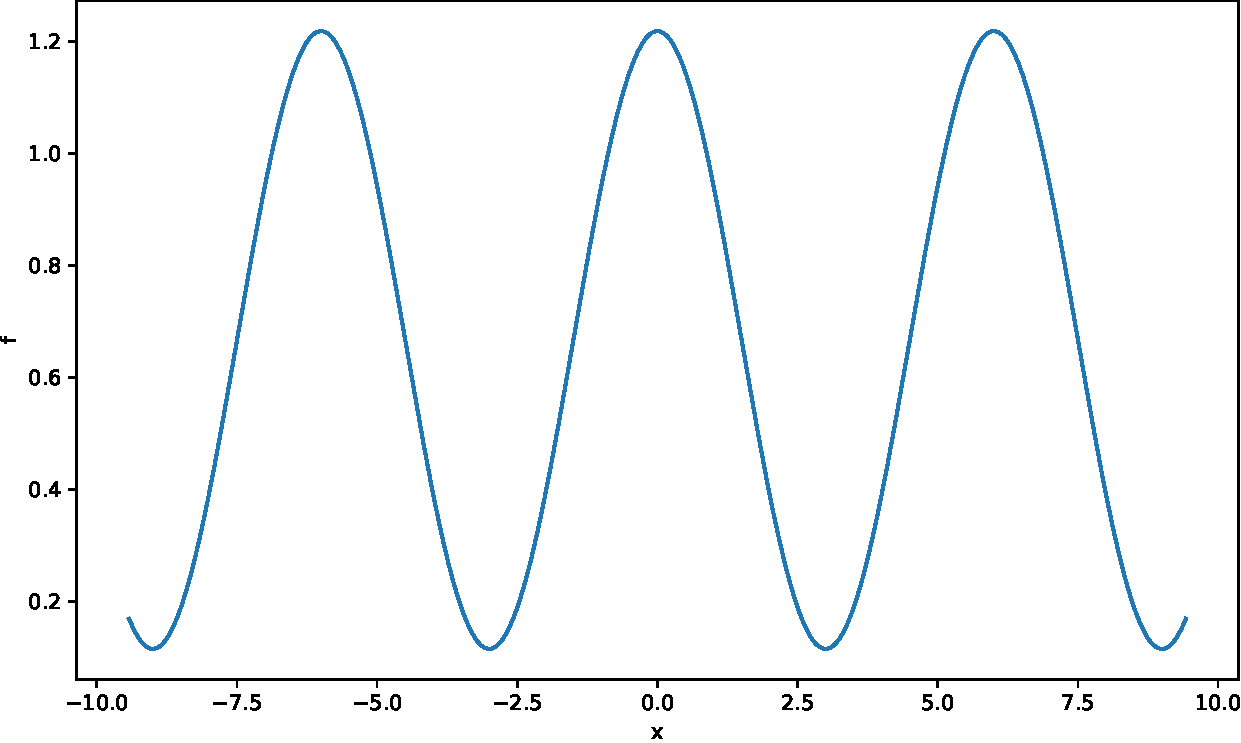
\includegraphics[width=\textwidth]{FourierSeries/Ex1.2.pdf}
		\caption{$N=2$}
	\end{subfigure}
	\hfill
	\begin{subfigure}[b]{0.49\textwidth}
		\centering
		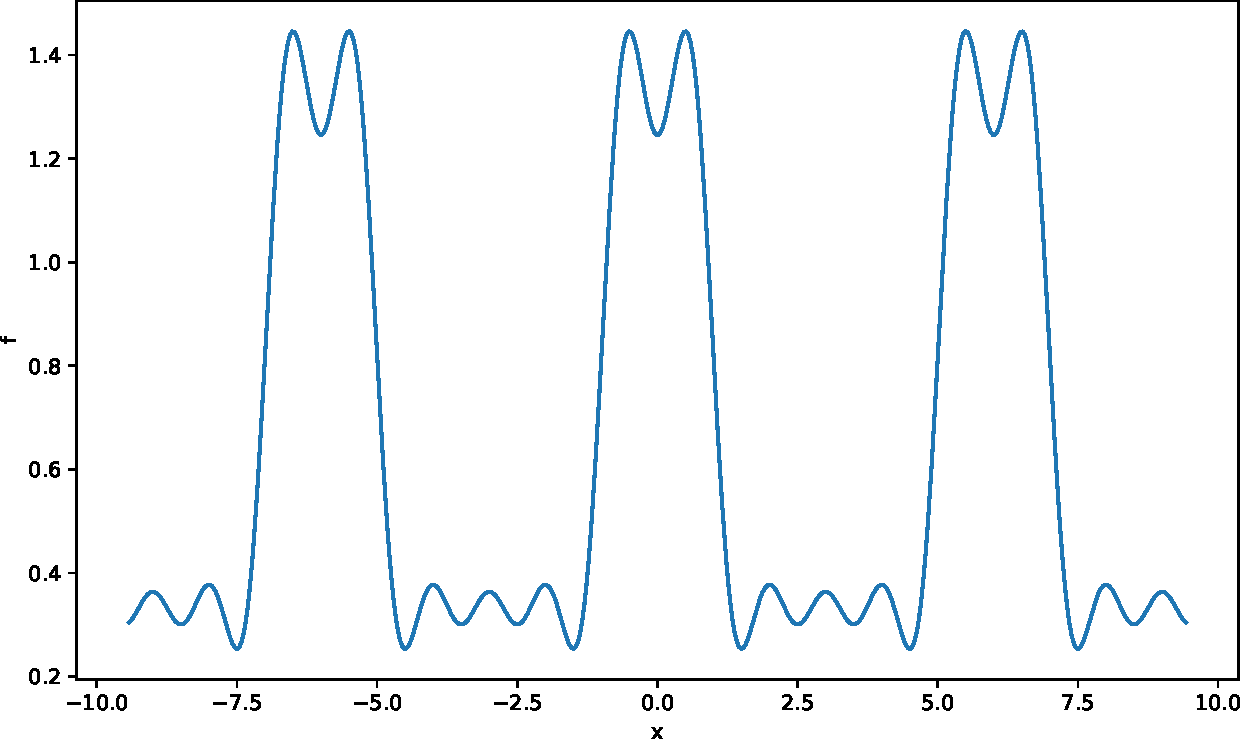
\includegraphics[width=\textwidth]{FourierSeries/Ex1.6.pdf}
		\caption{$N=6$}
	\end{subfigure}
	\\
	\begin{subfigure}[b]{0.49\textwidth}
		\centering
		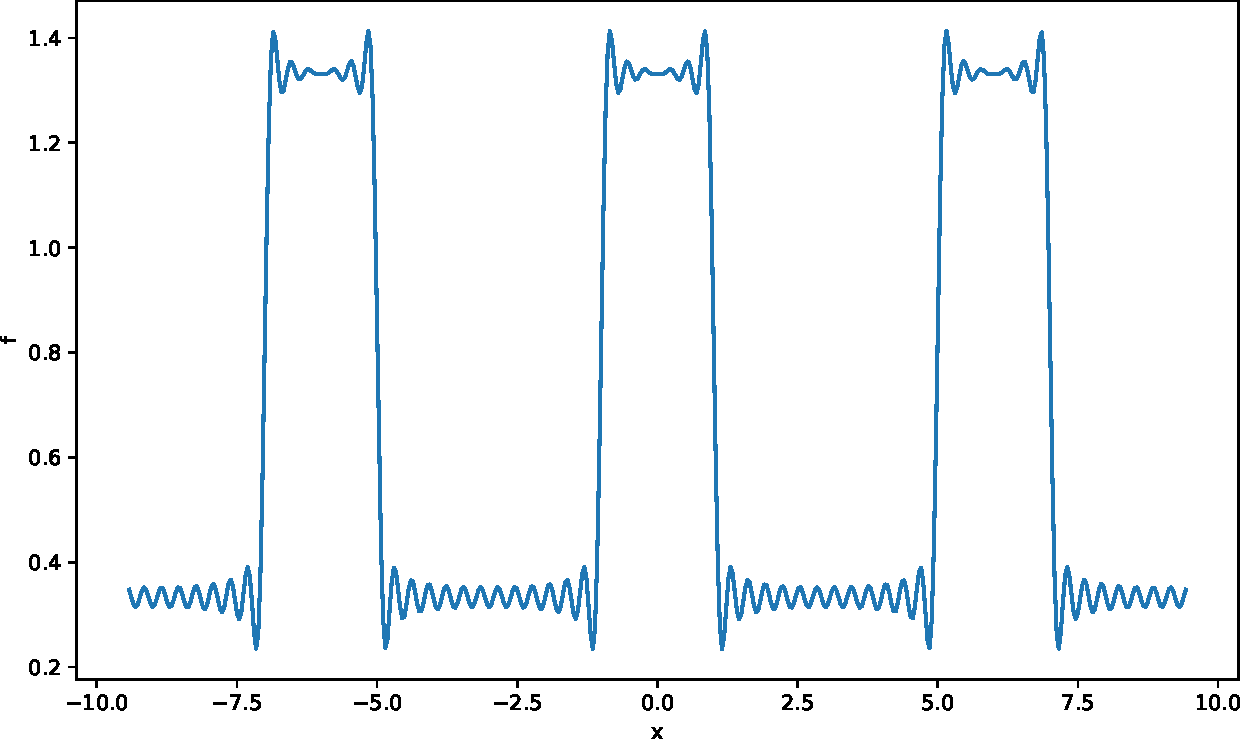
\includegraphics[width=\textwidth]{FourierSeries/Ex1.20.pdf}
		\caption{$N=20$}
	\end{subfigure}
	\hfill
	\begin{subfigure}[b]{0.49\textwidth}
		\centering
		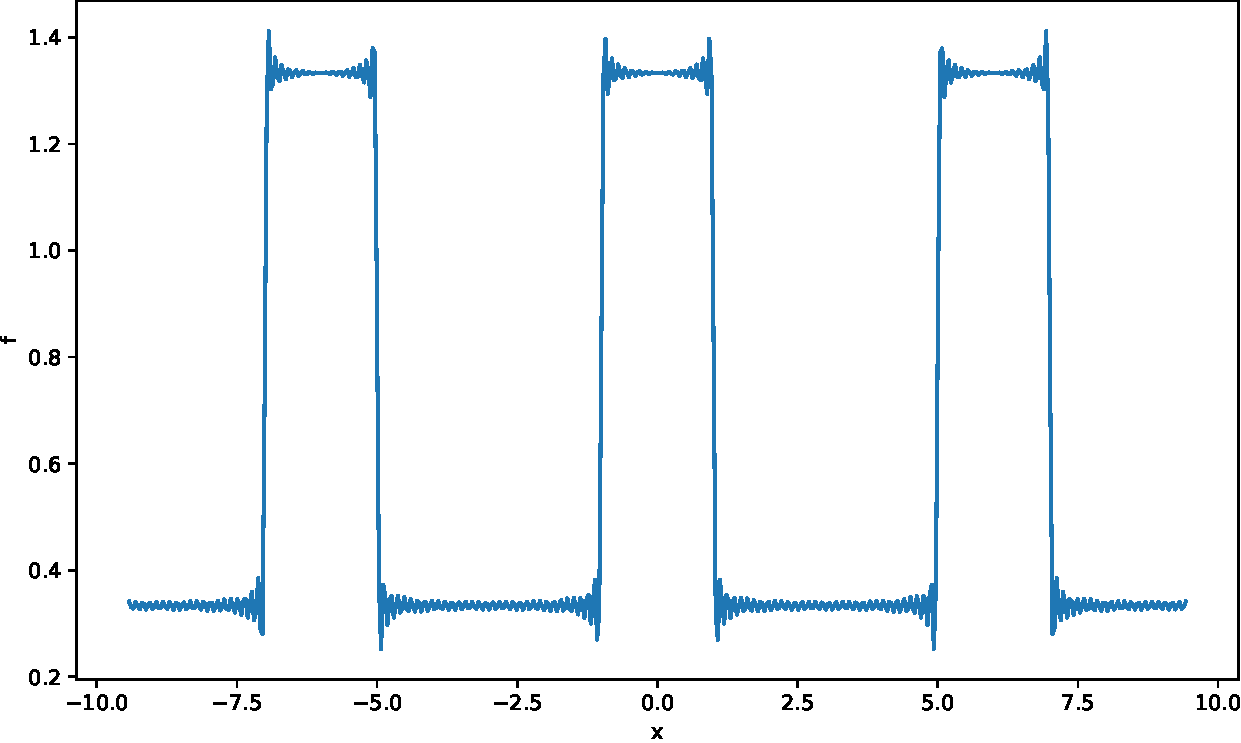
\includegraphics[width=\textwidth]{FourierSeries/Ex1.50.pdf}
		\caption{$N=50$}
	\end{subfigure}
	\caption{Truncated Fourier series from \Cref{eg:fourier1} with various values of $N$.}
	\label{fig:fourieregsub}
\end{figure}

\subsection{Fourier Convergence Theorem}

\begin{definition}
	A function $f$ is piecewise continuous on $[a,b]$ if there exists a finite number of points $a = x_0 < x_1 < \cdots < x_n = b$ such that
	\begin{itemize}
		\item $f$ is continuous on $(x_i, x_{i+1})$,
		\item $\lim_{x \to x_i^{\pm}} f(x) = c_i^{\pm} < \infty$ ($f(x)$ has a finite limit at the endpoints of each subinterval).
	\end{itemize}
\end{definition}

\begin{theorem}[Fourier Convergence Theorem]\label{thrm:fourierconv}
	Assume $f$ and $f'$ are piecewise continuous on $(-L,L)$ and $f(x+2L)=f(x)$. Then the Fourier series
	\[
	\frac{a_0}{2} + \sum_{n=1}^{\infty} \left(a_n \cos{\left(\frac{n\pi x}{L}\right)} + b_n \sin{\left(\frac{n\pi x}{L}\right)}\right)
	\]
	converges to
	\begin{itemize}
		\item $f(x)$ where $f$ is continuous,
		\item $\frac12 \left(\lim_{x\to x_i^-} f(x) + \lim_{x\to x_i^+} f(x)\right)$ where $f$ is discontinuous.
	\end{itemize}
\end{theorem}

\begin{remark}
	Functions like $\frac{1}{x^2}$ and $\log{x}$ have no convergent Fourier series because of the infinite divergences of the function at $x=0$ (so they are not piecewise continuous).
\end{remark}

\begin{remark}
	Functions with an infinite number of discontinuities are not guaranteed to have a convergent Fourier series.
\end{remark}

\begin{eg}[Square wave]\label{eg:squarewave}
	We consider the square wave function
	\[
	f(x) = \begin{cases}0 & \text{if } -L<x<0 \\ L & \text{if } 0<x<L\end{cases}
	\]
	From the Euler-Fourier formulas (\Cref{eq:eulerfourier1,eq:eulerfourier2,eq:eulerfourier3}), we can see that
	\[
	a_0 = \frac{1}{L} \int_{-L}^L f(x) \,dx = \frac{1}{L} \int_0^L L \,dx = L.
	\]
	Next, we find the coefficients $a_n$,
	\begin{align*}
		a_n &= \frac{1}{L} \int_{-L}^L f(x)\cos\left(\frac{n\pi x}{L}\right) dx = \frac{1}{L} \int_0^L L\cos\left(\frac{n\pi x}{L}\right) dx \\
		&= \frac{1}{L} \left[\frac{L^2}{n\pi} \sin\left(\frac{n\pi x}{L}\right)\right]_0^L = 0.
		\intertext{Finally, we find the $b_n$ terms,}
		b_n &= \frac{1}{L} \int_{-L}^L f(x)\sin\left(\frac{n\pi x}{L}\right) dx = \frac{1}{L} \int_0^L \sin\left(\frac{n\pi x}{L}\right) dx \\
		&= -\frac{1}{L} \left[\frac{L}{n\pi} \cos\left(\frac{n\pi x}{L}\right)\right]_0^L = \frac{1}{L} \frac{L^2}{n\pi}(1-\cos(n\pi)) \\
		&= \frac{L}{n\pi}(1-(-1)^n) = \begin{cases}0 & \text{if } n=2m \\ \frac{2L}{(2m+1)\pi} & \text{if } n=2m+1\end{cases}.
	\end{align*}
	Therefore the Fourier series is
	\[
	f(x) = \frac{L}{2} + \frac{2L}{\pi} \sum_{m=0}^{\infty} \frac{1}{2m+1} \sin\left(\frac{(2m+1)\pi x}{L}\right).
	\]
	By the Fourier Convergence Theorem (\Cref{thrm:fourierconv}), the series is convergent at all points where $f$ is continuous (which is everywhere where $x \neq nL$ for $n \in \Z$). At the discontinuities, we will have that the series tends to $\frac{L}{2}$, which is clear in the $x=0$ case as $\sin\left(\frac{(2m+1)\pi x}{L}\right)$ will be zero for all $m$.
\end{eg}

\subsubsection{Errors for Truncated Series}

As we saw in \Cref{fig:fourieregsub}, in practice it is not possible to work with an infinite series, so we must truncate the series taking only the terms up to some finite $N$, i.e. a partial sum:
\[
S_N = \frac{a_0}{2} + \sum_{n=1}^N \left(a_n \cos{\left(\frac{n\pi x}{L}\right)} + b_n \sin{\left(\frac{n\pi x}{L}\right)}\right).
\]
We define the error as
\[
e_N = S_N(x) - f(x),
\]
then we can investigate these in Python. Returning to the square wave from \Cref{eg:squarewave}, we can see that as $N$ increases,
\begin{itemize}
	\item The oscillations near the discontinuities get smaller in amplitude and wavelength.
	\item But the amplitude of the largest oscillation (nearest the discontinuity) does not decrease.
\end{itemize}

This occurrence of the largest oscillation not decreasing in amplitude is called \textbf{Gibbs Phenomenon}. This phenomenon is illustrated in \Cref{fig:gibbs} for the series in \Cref{eg:squarewave} with $L=1$.

\begin{figure}[!ht]
	\centering
	\begin{subfigure}[b]{0.49\textwidth}
		\centering
		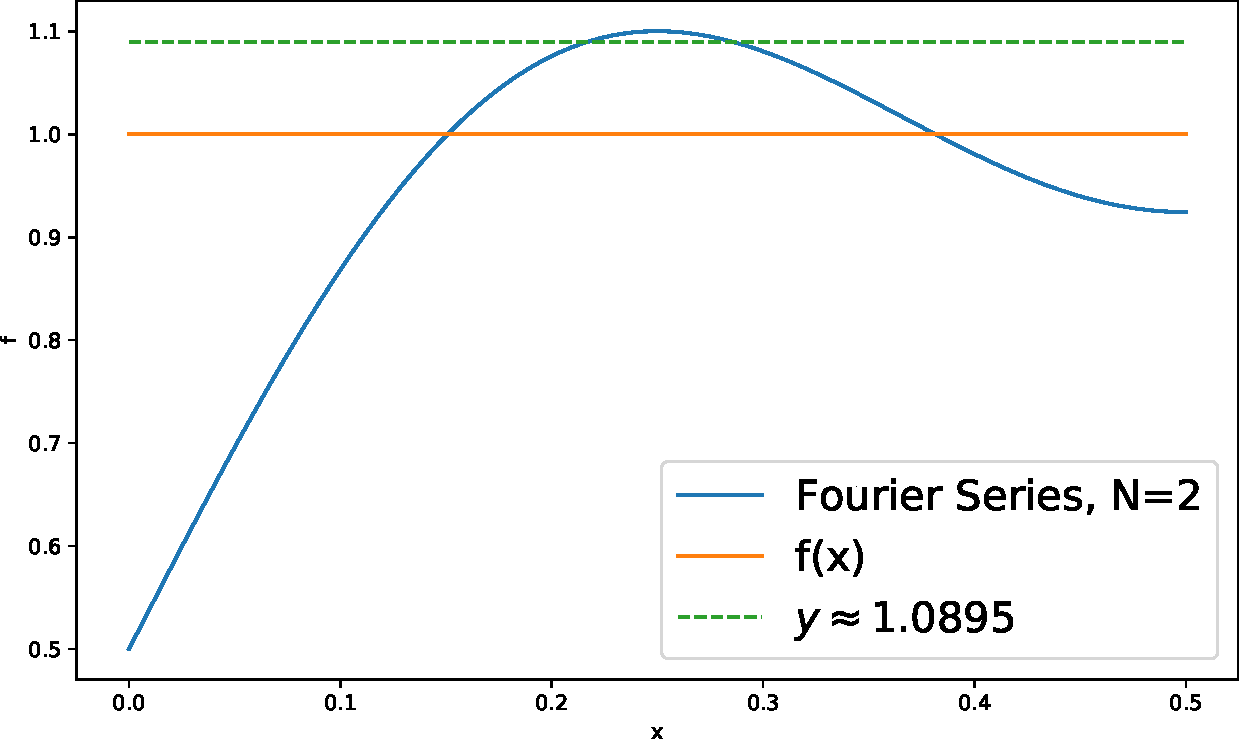
\includegraphics[width=\textwidth]{FourierSeries/Gibbs2.pdf}
		\caption{$N=2$}
	\end{subfigure}
	\hfill
	\begin{subfigure}[b]{0.49\textwidth}
		\centering
		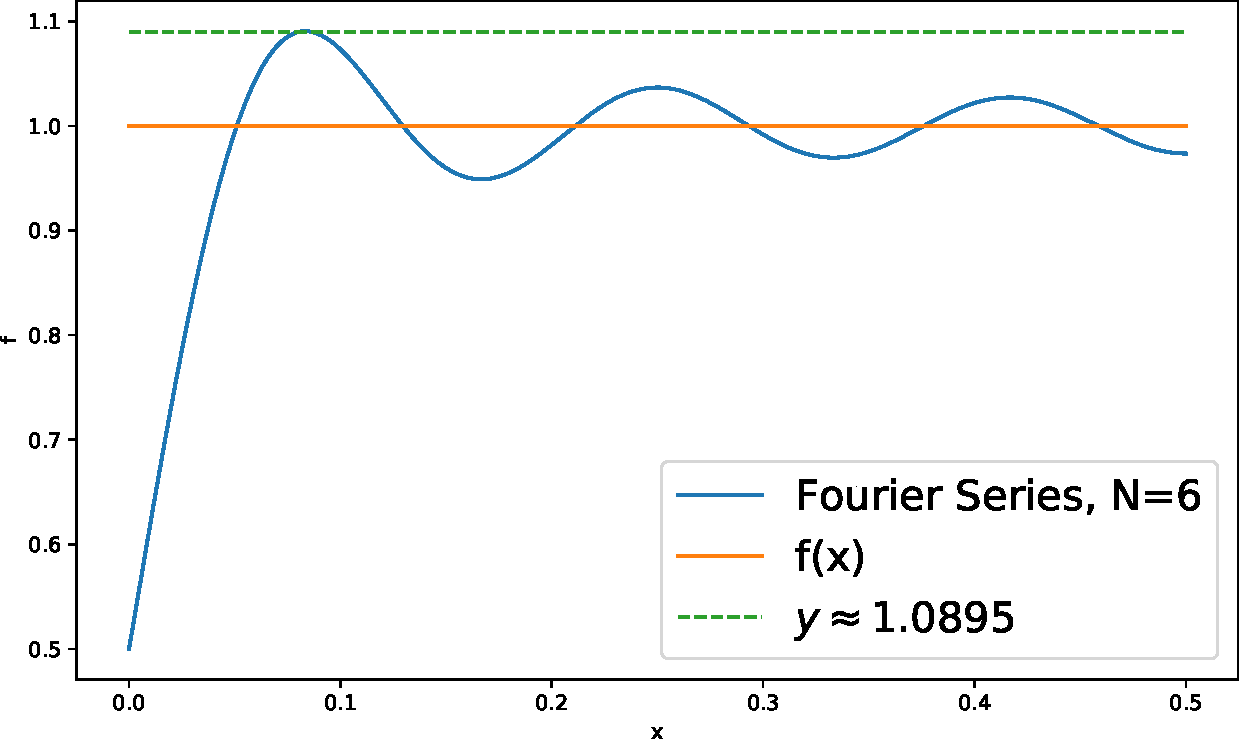
\includegraphics[width=\textwidth]{FourierSeries/Gibbs6.pdf}
		\caption{$N=6$}
	\end{subfigure}
	\\
	\begin{subfigure}[b]{0.49\textwidth}
		\centering
		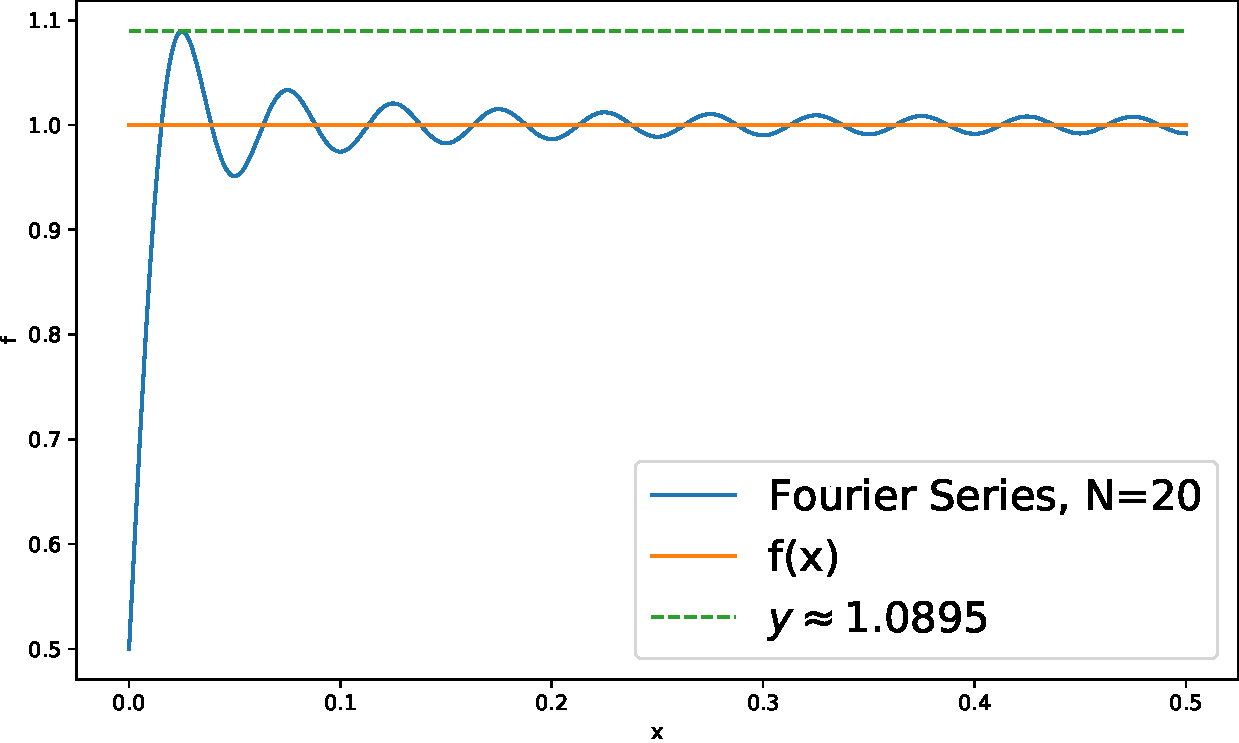
\includegraphics[width=\textwidth]{FourierSeries/Gibbs20.pdf}
		\caption{$N=20$}
	\end{subfigure}
	\hfill
	\begin{subfigure}[b]{0.49\textwidth}
		\centering
		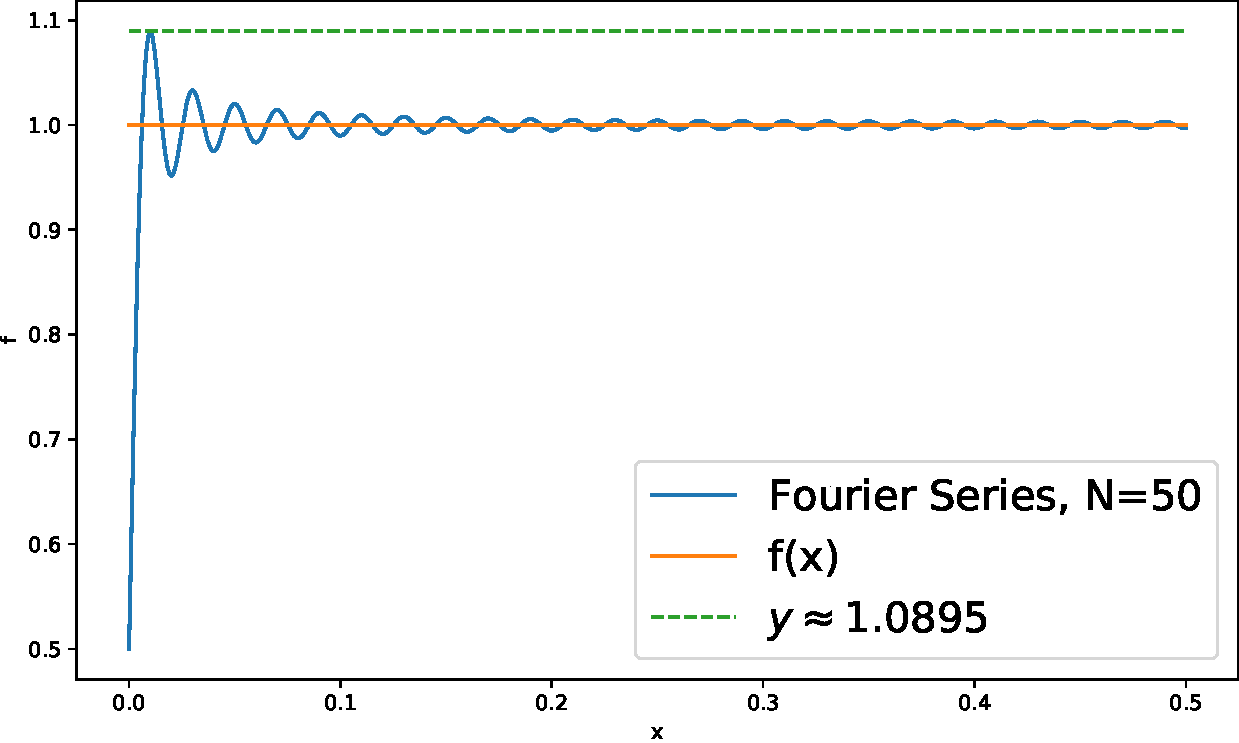
\includegraphics[width=\textwidth]{FourierSeries/Gibbs50.pdf}
		\caption{$N=50$}
	\end{subfigure}
	\caption{For the Fourier series from the square wave example with $L=1$, we observe that the maximum amplitude of the error around $x=0$ does not decrease as $N$ increases. Instead, it tends to a value of approximately 0.0895.\protect\footnotemark}
	\label{fig:gibbs}
\end{figure}

\footnotetext{In fact, we can calculate the error to be \[\frac{1}{\pi} \int_0^{\pi}\frac{\sin t}{t}dt - \frac12 = 0.089489877236\ldots \tag{\href{https://oeis.org/A243268}{OEIS A243268}}\] For a full derivation of this result, see \href{https://en.wikipedia.org/wiki/Gibbs_phenomenon}{Wikipedia}.}

\subsection{Other Results on Fourier Series}

\subsubsection{Complex Form}\label{sec:fouriercomplex}

Now we will see that we can write the Fourier series in \Cref{def:fourier} in terms of complex exponentials instead of trigonometric functions. This will make use of the fact that
\[
\cos(x) = \frac{e^{ix} + e^{-ix}}{2} \quad \text{and} \quad \sin(x) = \frac{e^{ix} - e^{-ix}}{2i}.
\]

For simplicity in the following derivation, we shall denote the argument of the trig functions by $k = \frac{n\pi x}{L}$.

\begin{align*}
	f(x) &= \frac{a_0}{2} + \sum_{n=1}^{\infty} \left(a_n \cos{\left(\frac{n\pi x}{L}\right)} + b_n \sin{\left(\frac{n\pi x}{L}\right)}\right) \\
	&= \frac{a_0}{2} + \sum_{n=1}^{\infty} \left(a_n \frac{e^{ik} + e^{-ik}}{2} + b_n \frac{e^{ik} - e^{-ik}}{2i}\right) \\
	&= \frac{a_0}{2} + \sum_{n=1}^{\infty} \frac{a_n - ib_n}{2} e^{ik} + \sum_{n=1}^{\infty} \frac{a_n + ib_n}{2} e^{-ik} \\
	&= \sum_{n=-\infty}^{\infty} c_n e^{in\pi x/L},
\end{align*}
where
\[
c_0 = \frac{a_0}{2}, \quad c_n = \frac{a_n - ib_n}{2}, n>0 \quad c_n = \frac{a_n + ib_n}{2}, n<0.
\]
Thus, we have formulas to convert real coefficients into complex coefficients. In addition, to convert complex coefficients into real coefficients, we can use the following formulas
\[
a_0 = 2c_0, \quad a_n = c_n + c_{-n}, \quad b_n = i(c_n - c_{-n}).
\]

To compute complex coefficients directly, we can use the Euler-Fourier formulas (\Cref{eq:eulerfourier1,eq:eulerfourier2,eq:eulerfourier3}), we find that
\begin{equation}\label{eq:fouriercomplexcoeffs}
	c_n = \frac{1}{2L} \int_{-L}^L f(x) e^{-in\pi x/L} \,dx.
\end{equation}

An alternative derivation of this formula for the $c_n$ terms is as follows: We have that
\[
f(x) = \sum_{n=-\infty}^{\infty} c_n e^{in\pi x/L}.
\]
We define a slightly different inner product from the one for real functions in \Cref{eq:innerprod}:
\begin{equation}\label{eq:innerprodcomplex}
	\left(u(x), v(x)\right) = \int_{-L}^L u(x)v^*(x) \,dx,
\end{equation}
where $v^*(x)$ is the complex conjugate of $v(x)$. From this definition, observe that
\[
\left(e^{in\pi x/L}, e^{im\pi x/L}\right) = 2L\delta_{mn},
\]
which we find using the new definition of the inner product,
\begin{align*}
	\left(e^{in\pi x/L}, e^{im\pi x/L}\right) &= \int_{-L}^L e^{in\pi x/L}e^{-im\pi x/L} \,dx \tag{$n \neq m$} \\
	&= \left[ \frac{Le^{i(n-m)\pi x/L}}{i(n-m)\pi} \right]_{-L}^L \\
	&= \frac{L}{i(n-m)\pi} \left(e^{ik\pi} - e^{-ik\pi}\right) \tag{$k=n-m$} \\
	&= \cos(k\pi) + i\sin(k\pi) - \cos(-k\pi) - i\sin(-k\pi) = 0.
\end{align*}
And for $n=m$,
\begin{align*}
	(e^{in\pi x/L}, e^{in\pi x/L}) &= \int_{-L}^L e^{in\pi x/L}e^{-in\pi x/L} \,dx \\
	&= \int_{-L}^L dx = 2L.
\end{align*}
Therefore the functions $e^{in\pi x/L}$ are orthogonal for all $n$, hence they form a basis. Finally, we can find the formula for $c_n$:
\begin{align*}
	\left(f(x), e^{im\pi x/L}\right) &= \sum_n c_n \cancelto{2L\delta_{mn}}{(e^{in\pi x/L}, e^{im\pi x/L})} = 2L c_m \\
	\implies c_m &= \frac{1}{2L} \int_{-L}^L f(x) e^{-im\pi x/L} \,dx.
\end{align*}

\begin{remark}
	While we now have the option to expand functions either in terms of $\sin$ and $\cos$ or complex exponentials, in practice it is usually easier to use the trig functions for real functions and exponentials for complex functions.
\end{remark}

\begin{eg}
	Using complex form, find the Fourier series of the function
	\[
	f(x) = \text{sgn}\,x = \begin{cases} -1 & \text{if } -\pi \leq x \leq 0 \\ 1 & \text{if } 0 < x \leq \pi \end{cases}.
	\]
	Calculating the coefficient $c_0$:
	\[
	c_0 = \frac{1}{2\pi} \int_{-\pi}^{\pi} f(x) \,dx = 0,
	\]
	since $f$ is an odd function. Next, we find the coefficients $c_n$:
	\begin{align*}
		c_n &= \frac{1}{2\pi} \int_{-\pi}^{\pi} f(x){e^{-inx}}dx \\
		&= \frac{1}{2\pi}\left[ \int_{-\pi}^0 \left( {-1} \right){e^{-inx}}dx + \int_0^{\pi} e^{-inx}dx \right] \\
		&= \frac{1}{2\pi} \begin{bmatrix} -\dfrac{\left. \left( e^{-inx} \right) \right|_{-\pi }^0}{-in} + \dfrac{\left. \left( e^{-inx} \right) \right|_0^\pi }{-in} \end{bmatrix} \\
		&= \frac{i}{2\pi n}\left[-\left(1-e^{in\pi} \right) + e^{-in\pi}-1 \right] \\
		&= \frac{i}{2\pi n}\left[e^{in\pi} + e^{-in\pi}-2 \right] = \frac{i}{\pi n} \begin{bmatrix} \dfrac{e^{in\pi} + e^{-in\pi}}{2}-1 \end{bmatrix} \\
		&= \frac{i}{\pi n}\left[\cos(n\pi)-1\right] = \frac{i}{\pi n}\left[(-1)^n-1\right].
	\end{align*}
	If $n=2k$, we have that $c_n = 0$, and if $n=2k-1$, $c_n = -\frac{2i}{(2k-1)\pi}$. Hence, we can write the Fourier series in complex form as
	\[
	f(x) = -\frac{2i}{\pi} \sum_{k=-\infty}^{\infty} \frac{1}{2k-1}e^{i(2k-1)x}.
	\]
\end{eg}

\subsubsection{Even and Odd Functions}\label{sec:evenoddfourier}

Recall the definitions of even and odd functions:
\begin{itemize}
	\item Even function: $f(x) = f(-x)$.
	\item Odd function: $f(x) = -f(-x)$.
\end{itemize}

First, we calculate the Fourier coefficients where $f$ is an even function:
\begin{align*}
	a_n &= \frac{1}{L} \int_{-L}^L f(x)\cos\left(\frac{n\pi x}{L}\right) dx \\
	&= \frac{1}{L} \left(\int_{-L}^0 f(x)\cos\left(\frac{n\pi x}{L}\right) dx + \int_0^L f(x)\cos\left(\frac{n\pi x}{L}\right) dx\right) \\
	&= \frac{2}{L} \int_0^L f(x)\cos\left(\frac{n\pi x}{L}\right) dx,
\end{align*}
since $f(x)\cos\left(\frac{n\pi x}{L}\right)$ is an even function, and
\[
b_n = \frac{1}{L} \int_{-L}^L f(x)\sin\left(\frac{n\pi x}{L}\right) = 0,
\]
since the integrand $f(x)\sin\left(\frac{n\pi x}{L}\right)$ is an odd function and the limits of integration are symmetric.

Similarly, the Fourier coefficients for an odd function are found to be
\[
a_n = 0 \quad b_n = \frac{2}{L} \int_0^L f(x)\sin\left(\frac{n\pi x}{L}\right) dx.
\]

Therefore, the Fourier series for an odd function will only be in terms of sines, and the series for an even function will contain only cosines.

\begin{eg}[Sawtooth Function]\label{eg:sawtooth}
	The sawtooth function is given by $f(x)=x$ for $-L\leq x<L$, with $f(x+2L) = f(x)$.
	
	Therefore, we have that $f$ is an odd function, therefore $a_n = 0$ for all $n$.
	
	Next, we find the $b_n$s using integration by parts
	\begin{align*}
		b_n &= \frac{2}{L} \int_0^L f(x)\sin\left(\frac{n\pi x}{L}\right) dx \\
		&= \frac{2}{L} \int_0^L x\sin\left(\frac{n\pi x}{L}\right) dx \\
		&= \frac{2}{L} \left(\left[ -\frac{xL}{n\pi}\cos\left(\frac{n\pi x}{L}\right) \right]_0^L + \frac{L}{n\pi}\cancelto{0}{\int_0^L \cos\left(\frac{n\pi x}{L}\right) dx} \right) \\
		&= -\frac{2}{L} \frac{L^2 (-1)^n}{n\pi} \tag{Since $\cos(n\pi) = (-1)^n$} \\
		&= \frac{2L}{n\pi}(-1)^{n+1}.
	\end{align*}
	Therefore the resulting Fourier series is
	\[
	f(x) = \frac{2L}{\pi} \sum_{n=1}^{\infty} \frac{(-1)^{n+1}}{n} \sin\left(\frac{n\pi x}{L}\right).
	\]
	The truncated Fourier series with the first 20 terms is shown in \Cref{fig:fouriersawtooth}.
\end{eg}

\begin{figure}[!ht]
	\centering
	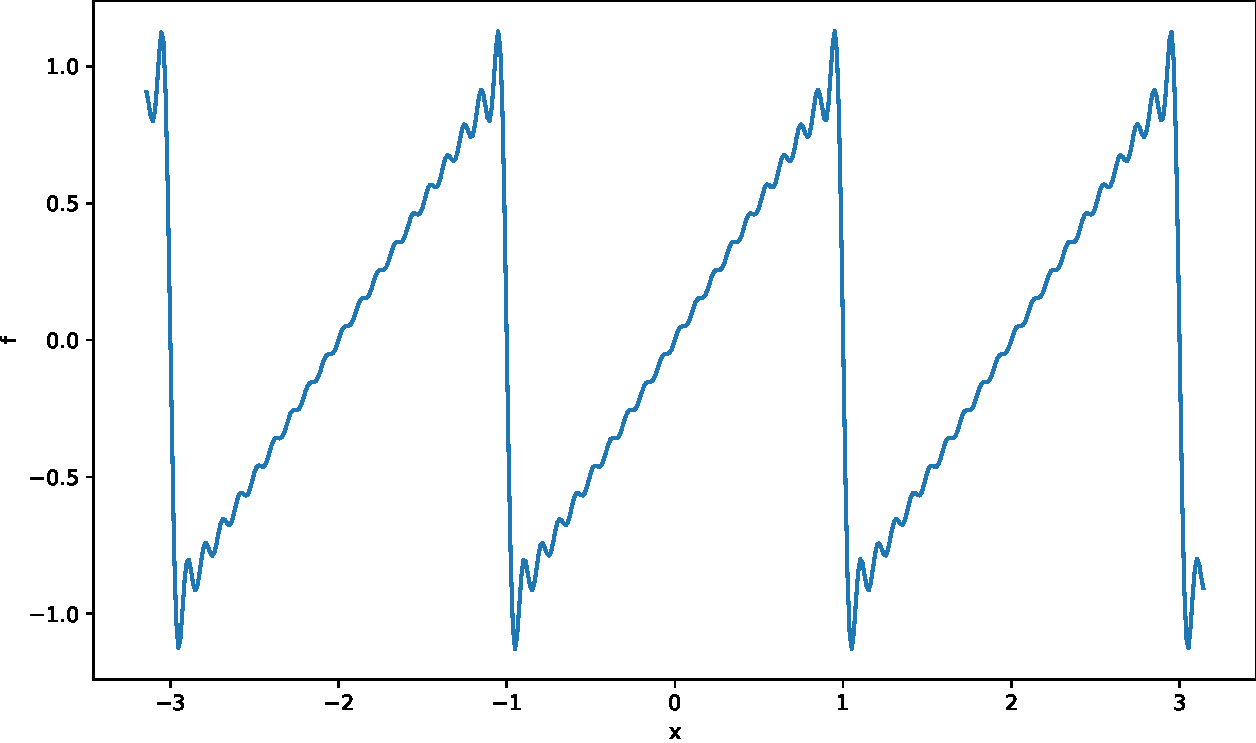
\includegraphics[width=0.7\textwidth]{FourierSeries/Sawtooth20.pdf}
	\caption{Fourier series for the sawtooth function in \Cref{eg:sawtooth} with first 20 terms.}
	\label{fig:fouriersawtooth}
\end{figure}

Note that we can still apply these formulas in the case where we have functions that are only defined on the interval $(0,L)$ by extending the function onto the interval $(-L,0)$ (then the periodicity condition $f(x+2L)=f(x)$ can be used to extend to the rest of the real line). The natural ways of doing this extension are the even extension and the odd extension, as in \Cref{fig:evenoddextension}.

\begin{figure}[!ht]
	\centering
	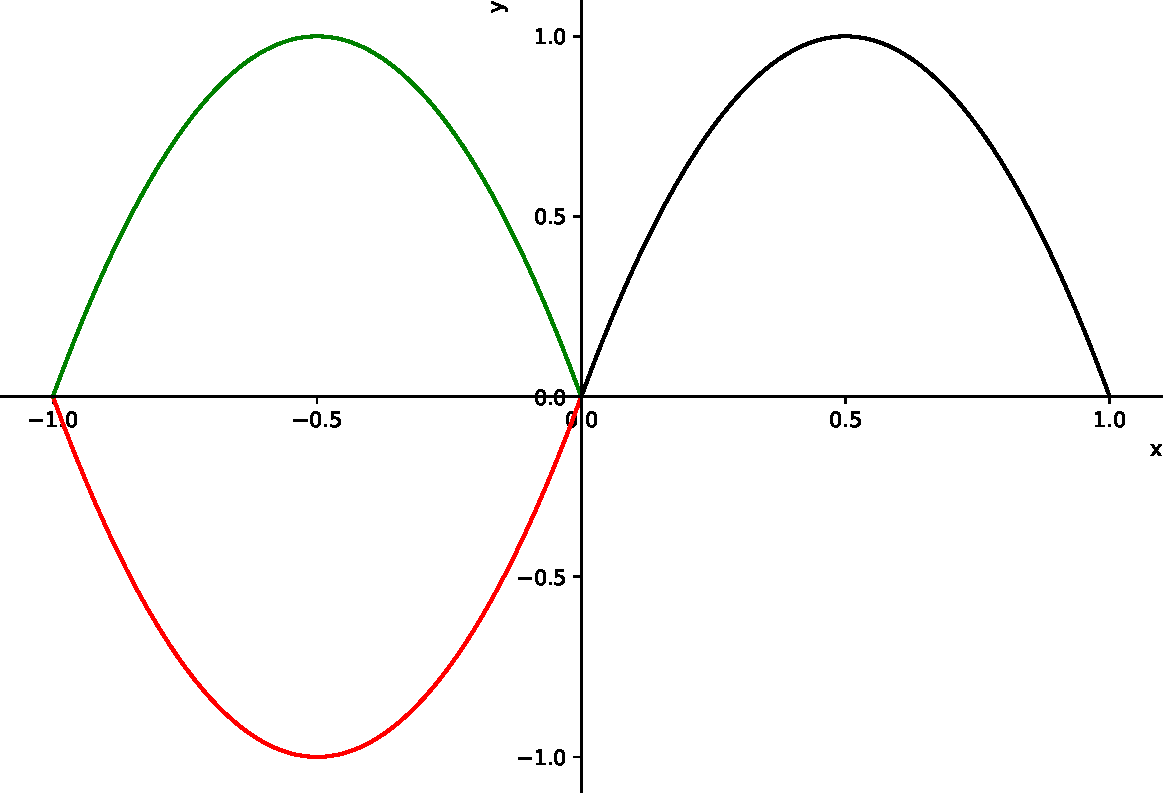
\includegraphics[width=0.6\textwidth]{EvenOddExtension.pdf}
	\caption{The function $f(x) = 4x(1-x)$ (black), with its even (green) and odd (red) extensions.}
	\label{fig:evenoddextension}
\end{figure}

Algebraically, given some function $f(x)$ for $x \in [0,L]$,
\begin{itemize}
	\item Its even extension can be defined as
	\[
		h(x) = \begin{cases}
			f(x) & x \in [0,L] \\
			f(-x) & x \in [-L,0]
		\end{cases}
	\]
	This will have a cosine series.
	\item Its odd extension can be defined as
	\[
	h(x) = \begin{cases}
		f(x) & x \in (0,L) \\
		0 & x = -L,0,L \\
		f(-x) & x \in (-L,0)
	\end{cases}
	\]
	This will have a sine series.
\end{itemize}

\subsubsection{Parseval's Theorem}

\begin{theorem}[Parseval's Theorem]\label{thrm:parseval}
	Suppose $f$ is a square integrable function on $[-L,L]$ (i.e. $f$ and $f^2$ are integrable on this interval) with the Fourier series
	\[
	f(x) = \frac{a_0}{2} + \sum_{n=1}^{\infty} \left(a_n \cos{\left(\frac{n\pi x}{L}\right)} + b_n \sin{\left(\frac{n\pi x}{L}\right)}\right)
	\]
	Then
	\[
	\lVert f\rVert^2 = (f,f) = \int_{-L}^L f^2(x) \,dx = 2L\sum_{n=-\infty}^{\infty} |c_n|^2 = L\left(\frac{a_0^2}{2} + \sum_{n=1}^{\infty}(a_n^2 + b_n^2)\right).
	\]
\end{theorem}

\begin{proof}
	We prove this theorem using the complex form of the Fourier series, as introduced in \Cref{sec:fouriercomplex}.
	\begin{align*}
		\lVert f\rVert^2 = (f,f) &= \left(\sum_n c_n e^{in\pi x/L}, \sum_m c_m e^{im\pi x/L}\right) \\
		&= \sum_n \sum_m c_n c_m^* \cancelto{2L\delta_{mn}}{(e^{in\pi x/L}, e^{im\pi x/L})} \\
		&= \sum_n c_n c_m^* 2L = 2L \sum_n |c_n|^2.
	\end{align*}
	Applying the relationships between $a_n$, $b_n$, and $c_n$ in \Cref{eq:fouriercomplexcoeffs}, we have that, for $n\neq0$,
	\[
	|c_n|^2 = \left|\frac{a_n \mp ib_n}{2}\right|^2 = \left(\frac{a_n}{2}\right)^2 + \left(\frac{b_n}{2}\right)^2 = \frac14(a_n^2 + b_n^2)
	\]
	So
	\begin{align*}
		2L\sum_{n=-\infty}^{\infty} |c_n|^2 &= 2L\left( |c_0|^2 + \sum_{n=-\infty}^{-1} |c_n|^2 + \sum_{n=1}^{\infty} |c_n|^2 \right) \\
		&= 2L\left( \left(\frac{a_0}{2}\right)^2 + \sum_{n=-\infty}^{-1} \frac14(a_n^2 + b_n^2) + \sum_{n=1}^{\infty} \frac14(a_n^2 + b_n^2)\right) \\
		&= 2L\left(\frac{a_0^2}{4} + 2\sum_{n=1}^{\infty} \frac14(a_n^2 + b_n^2)\right) \\
		&= L\left(\frac{a_0^2}{2} + \sum_{n=1}^{\infty}(a_n^2 + b_n^2)\right).
	\end{align*}
\end{proof}

\begin{eg}
	We apply Parseval's Theorem to the sawtooth function in \Cref{eg:sawtooth}. Recall that we had the function $f(x) = x$ for $-L\leq x < L$, with corresponding Fourier series
	\[
	f(x) = \frac{2L}{\pi} \sum_{n=1}^{\infty} \frac{(-1)^{n+1}}{n} \sin\left(\frac{n\pi x}{L}\right).
	\]
	Then
	\[
	\lVert f \rVert^2 = (f,f) = \int_{-L}^L x^2 \,dx = \frac{2L^3}{3}
	\]
	by direct calculation. Now, applying Parseval's Theorem,
	\begin{align*}
		\frac{2L^3}{3} &= \int_{-L}^L f^2(x) \,dx = L \sum_{n=1}^{\infty} b_n^2 \\
		&= L \sum_{n=1}^{\infty} \frac{4L^2}{\pi^2} \frac{1}{n^2} \\
		\implies \frac{4L^3}{\pi^2} \sum_{n=1}^{\infty} \frac{1}{n^2} &= \frac{2L^3}{3} \\
		\implies \sum_{n=1}^{\infty} \frac{1}{n^2} &= \frac{\pi^2}{6}.
	\end{align*}
	This rather beautiful formula for the sum of the reciprocals of the square numbers was proved by Euler (though using a different method) and was known as the \href{https://en.wikipedia.org/wiki/Basel_problem}{Basel problem}.
\end{eg}
\section{PDEs by Separation of Variables}

This method works for linear PDEs whose variables are separable, i.e., PDEs for which some solutions can be written as products of functions of the two independent variables:
\[
u(x,t) = f(x)g(t)
\]

\subsection{The Heat Equation}

To give a bit of background about the heat equation:
\begin{itemize}
	\item The heat equation can be used to describe the evolution of temperature in a one-dimensional object. If we imagine a thin rod, its temperature will depend only on the position $x$ of the particles between $0$ and $L$, and the time $t$. \\
	The heat equation describes how this temperature changes as a function of time. As time evolves, the temperature differences across the rod decrease because the conduction of heat across the rod conducts energy from areas of high temperature to low temperature. In this case, we will take the boundary conditions of $u$ to be 0 when $x=0$ and $x=L$; this corresponds to setting the temperature to 0 at these ends.
	
	\item Similarly, the heat equation can also be applied to Brownian motion or random walks. It describes the probability density function of particles that move randomly according to Brownian movements. Brownian motion is the limit of a random walk where walkers take many steps in very short intervals of time. The boundary conditions in this case are the points where we get rid of particles that touch any end of the walk. So at $x=0$ and $x=L$ again.
\end{itemize}

The heat equation is given by 
\begin{equation}\label{eq5.1}
	\p_t u = \alpha^2 \p_{xx} u,
\end{equation} 
where $\alpha > 0$.

The boundary conditions are given by
\[
u(0,t) = u(L,t) = 0,
\]
and the initial conditions are given by
\[
u(x,0) = f(x).
\]
This corresponds to modelling the temperature in a rod given an initial temperature distribution $f(x)$ and where we set the temperature to zero at both ends of the rod, as shown in \Cref{fig:heateqnrod}.

\begin{figure}[!ht]
	\centering
	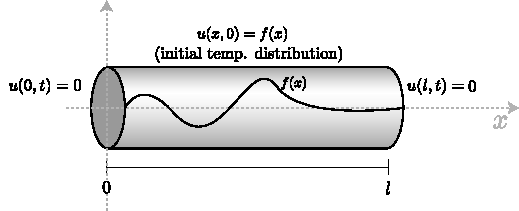
\includegraphics[width=0.7\textwidth]{HeatEqnRod.pdf}
	\caption{Modelling the temperature in a rod using the heat equation with homogeneous boundary conditions (source: \href{https://commons.wikimedia.org/wiki/File:Temp_Rod_homobc.svg}{Wikimedia}).}
	\label{fig:heateqnrod}
\end{figure}

We can solve the heat equation by separation of variables as follows: we look for solutions $u(x,t)$ as a product of two functions which have independent variables. So, try:
\begin{equation}\label{eq5.2}
	u(x,t) = X(x) T(t).
\end{equation}
Substituting \Cref{eq5.2} in \Cref{eq5.1}:
\begin{align*}
	XT' &= \alpha^2 X''T \\
	\implies \frac{1}{\alpha^2} \frac{T'}{T} &= \frac{X''}{X}.
\end{align*}
Now we have a function of only $x$ on the RHS and only $t$ on the LHS. This is possible only if $\frac{1}{\alpha^2} \frac{T'}{T} = \frac{X''}{X} = \lambda$ where $\lambda$ is a constant, called the separation constant. So, now we have two ODEs:
\[
X'' = \lambda X \quad\text{and}\quad T' = \lambda \alpha^2 T.
\]
To find solutions for $X(x)$, we have boundary conditions $X(0) = X(L) = 0$, so we now want non-trivial solutions to $X(x)$. What we have now is the eigenvalue problem from \Cref{sec:boundaryvalprob} where $\lambda$ is the eigenvalue.

We consider three cases:
\begin{itemize}
	\item Case 1: $\lambda = \mu^2 > 0$.\\
	The ODE is given by: $X'' - \mu^2X = 0$.\\
	In this case, the solution is given by:
	\[
	X(x) = A \cosh{\mu x} + B \sinh{\mu x}.
	\]
	Using the boundary values:
	\begin{align*}
		X(0) &= A = 0 \\
		X(L) &= B \sinh{\mu L} = 0 \implies B=0.
	\end{align*}
	So, there are only trivial solutions in this case.
	
	\item Case 2: $\lambda = 0$.\\
	The ODE is given by: $X''= 0$.\\
	In this case, the solution is given by:
	\[
	X(x) = Ax + B.
	\]
	Using the boundary values:
	\begin{align*}
		X(0) &= B = 0 \\
		X(L) &= AL = 0 \implies A = 0.
	\end{align*}
	So, there are only trivial solutions in this case.
	
	\item Case 3: $\lambda = -\mu^2 < 0$.\\
	The ODE is given by: $X'' + \mu^2 X = 0$.\\
	In this case, the solution is given by:
	\[
	X(x) = A \cos{\mu x} + B \sin{\mu x}.
	\]
	Using the boundary values:
	\begin{align*}
		X(0) &= A = 0 \\
		X(L) &= B \sin{\mu L} = 0.
	\end{align*}
	In this case, however, $B \neq 0$ if $\mu L = n \pi$ where $n \in \Z$. So, we have non-trivial solutions $\lambda = -\mu^2$ where $\mu = \frac{n \pi}{L}$.
\end{itemize}
Thus, the eigenvalues are given by: $\lambda = -\frac{n^2\pi^2}{L^2}$, where $n = 1, 2, \dots$, and the eigenfunctions are given by: $X_n(x) = \sin\left(\frac{n\pi x}{L}\right)$.

To find solutions for $T(t)$:
\begin{align*}
	T' &= \alpha^2 \lambda T \\
	T_n' &= -\frac{\alpha^2 n^2 \pi^2}{L^2} T_n \\ 
	\implies T_n(t) &= e^{-\alpha^2 n^2 \pi^2 t/L^2}.
\end{align*}
Therefore we have a linear set of solutions of the form:
\[
u_n(x,t) = X_n(x)T_n(t) = \sin\left(\frac{n\pi x}{L}\right) e^{-\alpha^2 n^2 \pi^2 t/L^2}
\]
To get a general solution, we use superposition:
\begin{equation}
	u(x,t) = \sum_{n=1}^{\infty} c_n e^{-\alpha^2 n^2 \pi^2 t/L^2} \sin\left(\frac{n\pi x}{L}\right).
\end{equation}
In order to satisfy the initial condition, we require
\[
u(x,0) = \sum_{n=1}^{\infty} c_n \sin\left(\frac{n\pi x}{L}\right) = f(x),
\]
which we observe is nothing but the Fourier series for an odd function (or odd extension). Using the Euler-Fourier formulas from \Cref{sec:evenoddfourier}, we have that
\begin{equation}\label{eq:heatfourier}
	c_n = \frac{2}{L} \int_0^L f(x)\sin\left(\frac{n\pi x}{L}\right) dx.
\end{equation}

\begin{eg}\label{eg:heateqn1}
	We solve the heat equation with boundary conditions given by: $u(0,t) = u(1,t) = 0$, and initial conditions $u(x,0) = f(x)$, where $f$ is the tent function given by
	\[
	f(x) = \begin{cases} 2x & \text{if } x \leq \frac12 \\ 2(1-x) & \text{if } x>\frac12 \end{cases}.
	\]
	Since $L=1$,\footnote{This derivation is done in more detail in \Cref{eg:laplacerect}.}
	\begin{align*}
		c_n &= 2 \int_0^1 f(x) \sin(n\pi x) \,dx \\
		&= 2 \int_0^{1/2} x \sin(n\pi x) \,dx + 2 \int_{1/2}^1 (1-x) \sin(n\pi x) \,dx \\
		&= \frac{4}{(n \pi)^2} \sin \left(\frac{n \pi}{2}\right) \\
		&= \begin{cases}0 & \text{if } n = 2k \\ \dfrac{4}{((2k+1)\pi)^2} (-1)^k & \text{if } n = 2k+1\end{cases}.
	\end{align*}
	Thus the solution is given by, 
	\[
	u(x,t) = \sum_{k=0}^{\infty} \frac{8}{((2k+1)\pi)^2} (-1)^k e^{-\alpha^2 n^2 \pi^2 t} \sin\left((2k+1)\pi x\right).
	\]
	This solution is shown in \Cref{fig:heateqneg1} for a few select values of $t$.
\end{eg}

\begin{figure}[!ht]
	\centering
	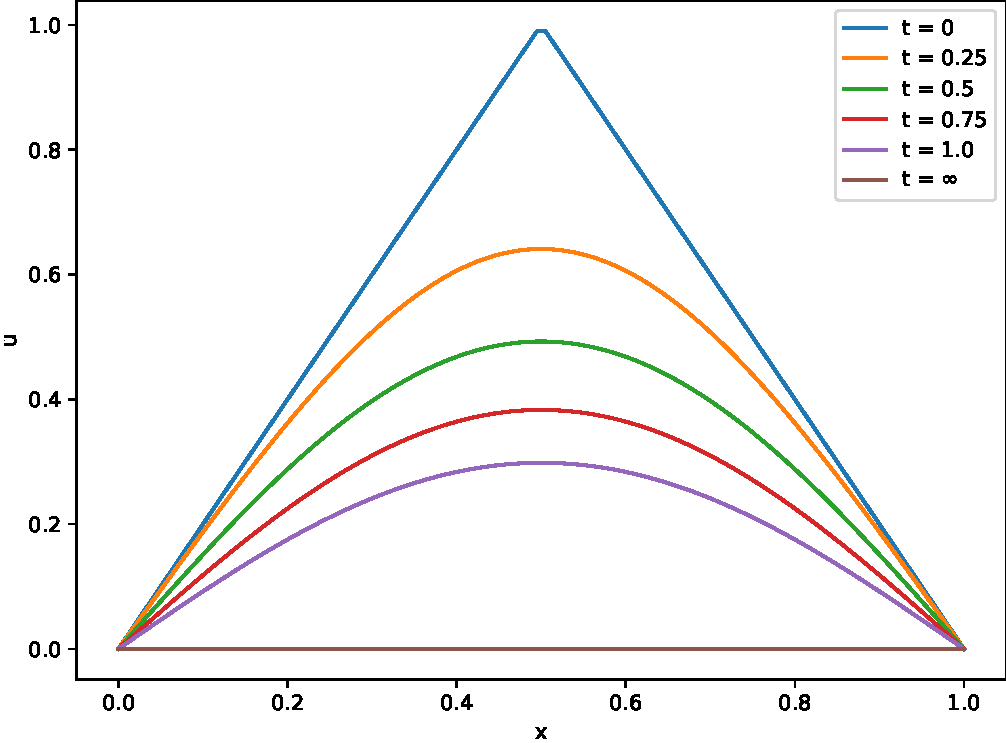
\includegraphics[width=0.7\textwidth]{HeatEqn1.pdf}
	\caption{Solution of the heat equation given the initial conditions in \Cref{eg:heateqn1}.}
	\label{fig:heateqneg1}
\end{figure}

\subsubsection{Non-homogenous Boundary Conditions}

We now wish to solve the heat equation 
\[
\p_t u = \alpha^2 \p_{xx} u
\]
with non-homogeneous (i.e. non-zero) boundary conditions:
\[
u(0,t) = a, \quad u(L,t) = b
\]
and initial condition
\[
u(x,0) = f(x).
\]
Let
\begin{equation}
	u(x,t) = v(x) + w(x,t),
\end{equation}
where $v(x)$ is a steady solution of the heat equation, meaning that it satisfies
\[
\p_{xx} v(x) = \frac{d^2}{dx^2} v = 0,
\]
and $v(0) = a$ and $v(L) = b$.
Since $u$ satisfies the heat equation, so do $v$ and $w$ by linearity of $u$. So,
\begin{align*}
	& \p_t u = \cancelto{0}{\p_t v(x)} + \p_t w(x,t) = \alpha^2 \left( \cancelto{0}{\p_{xx} v(x)} + \p_{xx} w \right)\\
	\implies & \p_t w(x,t) = \alpha^2 \p_{xx} w \\
	\implies & u(0,t) = v(0) + w(0,t) = a \\
	\implies & w(0,t) = 0.
\end{align*}
Similarly, we find that $w(L,t) = 0$.

Solving for $v(x)$:
\[
v'' = 0, \qquad v(0) = a, v(L) = b
\]
The solution is given by:
\begin{align*}
	v(x) &= Ax + B \\
	v(0) & = B = a \\
	v(L) & = AL + a = b \\
	\implies A &= \frac{b-a}{L}.
\end{align*}
So, we have
\[
v(x) = \frac{b-a}{L}x + a.
\]

Solving for $w(x,t)$, we know that $w(x,t)$ satisfies the heat equation with homogenous boundary conditions so 
\[
w(x,t) = \sum_{n=1}^{\infty} c_n e^{-\alpha^2 n^2 \pi^2 t/L^2} \sin\left(\frac{n\pi x}{L}\right),
\]
and
\begin{equation}
	u(x,t) = \frac{b-a}{L}x + a + \sum_{n=1}^{\infty} c_n e^{-\alpha^2 n^2 \pi^2 t/L^2} \sin\left(\frac{n\pi x}{L}\right).
\end{equation}
We now use the initial conditions at $t=0$, 
\begin{align*}
	u(x,0) &= f(x) \\
	v(x) + w(x,0) &= f(x) \\
	\implies w(x,0) &= f(x) - v(x).
\end{align*}
From \Cref{eq:heatfourier}, we have that 
\begin{equation}
	c_n = \frac{2}{L} \int_{-L}^L \left( f(x) - \frac{b-a}{L}x - a \right) \sin{\left(\frac{n \pi x}{L} \right)} dx.
\end{equation}

\begin{eg}\label{eg:heateqn2}
	Consider the heat equation
	\[
	\p_t u = \alpha^2 \p_{xx} u,
	\]
	given $L=1$ and boundary and initial conditions:
	\begin{align*}
		u(0,t) = 0 \\
		u(L,t) = 1 \\
		u(x,0) = 0.
	\end{align*} 
	Here, $v(x) = x$ since $b=1$, $a=0$, and $L=1$, so
	\[
	c_n = 2 \int_{0}^1 (-x) \sin{\left(n \pi x \right)} \,dx = \frac{2(-1)^n}{n \pi}.
	\]
	So the solution is
	\[
	u(x,t) = x + \frac{2}{\pi} \sum_{n=1}^{\infty} \frac{(-1)^n}{n} e^{-\alpha^2 n^2 \pi^2 t}\sin{\left(n \pi x \right)}.
	\]
	This solution is shown in \Cref{fig:heateqneg2} for a few select values of $t$.
\end{eg}

\begin{figure}[!ht]
	\centering
	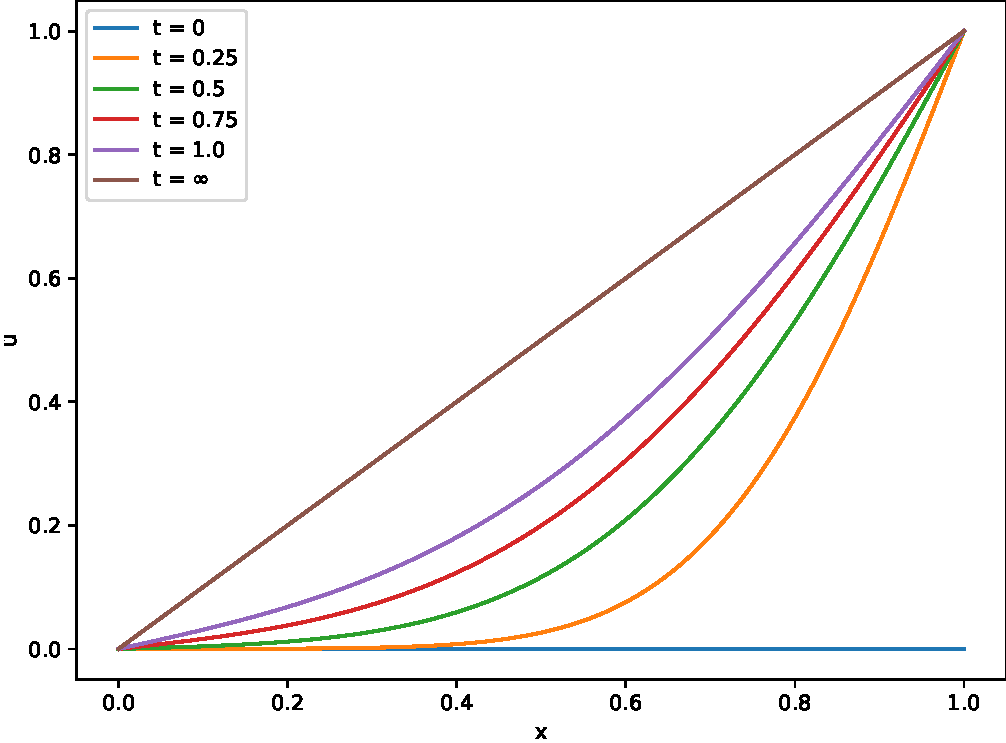
\includegraphics[width=0.7\textwidth]{HeatEqn2.pdf}
	\caption{Solution of the heat equation given the initial conditions in \Cref{eg:heateqn2}.}
	\label{fig:heateqneg2}
\end{figure}

\subsubsection{No-flux Boundary Conditions}

Finally, we wish to solve the heat equation
\[
\p_t u = \alpha^2 \p_{xx} u
\] 
with no-flux boundary conditions, i.e. where
\[
\p_x u(0,t) = \p_x u(L,t) = 0,
\]
and the typical initial conditions
\[
u(x,0) = f(x).
\]

Using the method of separation of variables:
\begin{align*}
	u(x,t) &= X(x) T(t) \\
	\frac{1}{\alpha^2} \frac{T'}{T} &= \frac{X''}{X} \\
	\implies X'' - \lambda X &= 0,
\end{align*}
where $X'(0) = X'(L) = 0$.

We then consider the separate cases of $\lambda$ as before:
\begin{itemize}
	\item Case 1: $\lambda = \mu^2 > 0$.\\
	The ODE is given by: $X(x)'' - \mu^2 X(x) = 0$.\\
	In this case, the solution is given by:
	\[
	X(x) = A \cosh{\mu x} + B \sinh{\mu x}.
	\]
	Using the boundary values:
	\begin{align*}
		X'(0) &= \mu B = 0 \implies B=0 \\
		X'(L) &= \mu A \cosh{\mu L} = 0 \implies A=0.
	\end{align*}
	So, there are only trivial solutions in this case.
	
	\item Case 2: $\lambda = 0$.\\
	The ODE is given by: $X''= 0$.\\
	In this case, the solution is given by:
	\[
	X(x) = Ax + B.
	\]
	Using the boundary values:
	\begin{align*}
		X'(0) &= A = 0 \\
		X'(L) &= AL = 0 \implies A = 0,
	\end{align*}
	which is true for all values of $B$. Therefore, the eigenvalue $\lambda_0 = 0$ has a corresponding eigenfunction given by $X(x) = 1$.
	
	\item Case 3: $\lambda = -\mu^2 < 0$.\\
	The ODE is given by: $X'' + \mu^2 X = 0$.\\
	In this case, the solution is given by:
	\[
	X(x) = A \cos{\mu x} + B \sin{\mu x}.
	\]
	Using the boundary values:
	\begin{align*}
		X'(0) &= \mu B = 0 \implies B = 0 \\
		X'(L) &= -\mu A \sin{\mu L} = 0 \implies \mu L = n \pi,
	\end{align*}
	where $n \in \Z \backslash \{0\} $. So, we have non-trivial solutions $\lambda = -\mu^2$ where $\mu = \frac{n \pi}{L}$.
\end{itemize}
Thus, the eigenvalues are given by: $\lambda_n = -\frac{n^2\pi^2}{L^2}$, and the eigenfunctions are given by: $X_n(x) = \cos{\left(\frac{n \pi x}{L} \right)}$.

Recall
\begin{align*}
	T' &= \lambda \alpha^2 T \\
	T_0(t) &= 1 \\
	T_n(t) &= e^{-\alpha^2 n^2 \pi^2 t/L^2}.
\end{align*}
So we have sets of solutions given by:
\[
u_n(x,t) = X_n(x) T_n(t) = \cos{\left(\frac{n \pi x}{L} \right)} e^{-\alpha^2 n^2 \pi^2 t/L^2}.
\]
By applying superposition, we can find the general solution to be:
\begin{equation}
	u(x,t) = \frac{c_0}{2} + \sum_{n=1}^{\infty} c_n e^{-\alpha^2 n^2 \pi^2 t/L^2} \cos{\left(\frac{n \pi x}{L} \right)}.
\end{equation}
Now considering the initial conditions:
\begin{align}
	u(x,0) & = f(x) \nonumber \\
	f(x) & = \frac{c_0}{2} + \sum_{n=1}^{\infty} c_n \cos{\left(\frac{n \pi x}{L} \right)} \nonumber \\
	\implies c_n & = \frac{2}{L} \int_0^L f(x) \cos{\left(\frac{n \pi x}{L} \right)} dx,
\end{align}
since this is nothing but the Fourier series for an even function.

\subsection{The Wave Equation}\label{sec:waveeqn}

We now solve another important partial differential equation: the wave equation,
\begin{equation}
	\p_{tt}u = a^2 \p_{xx}u, \quad a>0,
\end{equation}
where $a$ represents the wave speed.

In practice, this equation can be used to model a string under tension, or shallow water waves.

We will solve the equation with the following boundary conditions,
\[
u(0,t) = u(L,t) = 0,
\]
and the initial conditions
\[
u(x,0) = f(x), \quad \p_t u(x,0) = g(x).
\]
These conditions correspond to the wave being fixed at $u=0$ at both ends, with an initial position and initial speed at point $x$ given by $f(x)$ and $g(x)$, respectively (see \Cref{fig:wavestring}).

\begin{figure}[!ht]
	\centering
	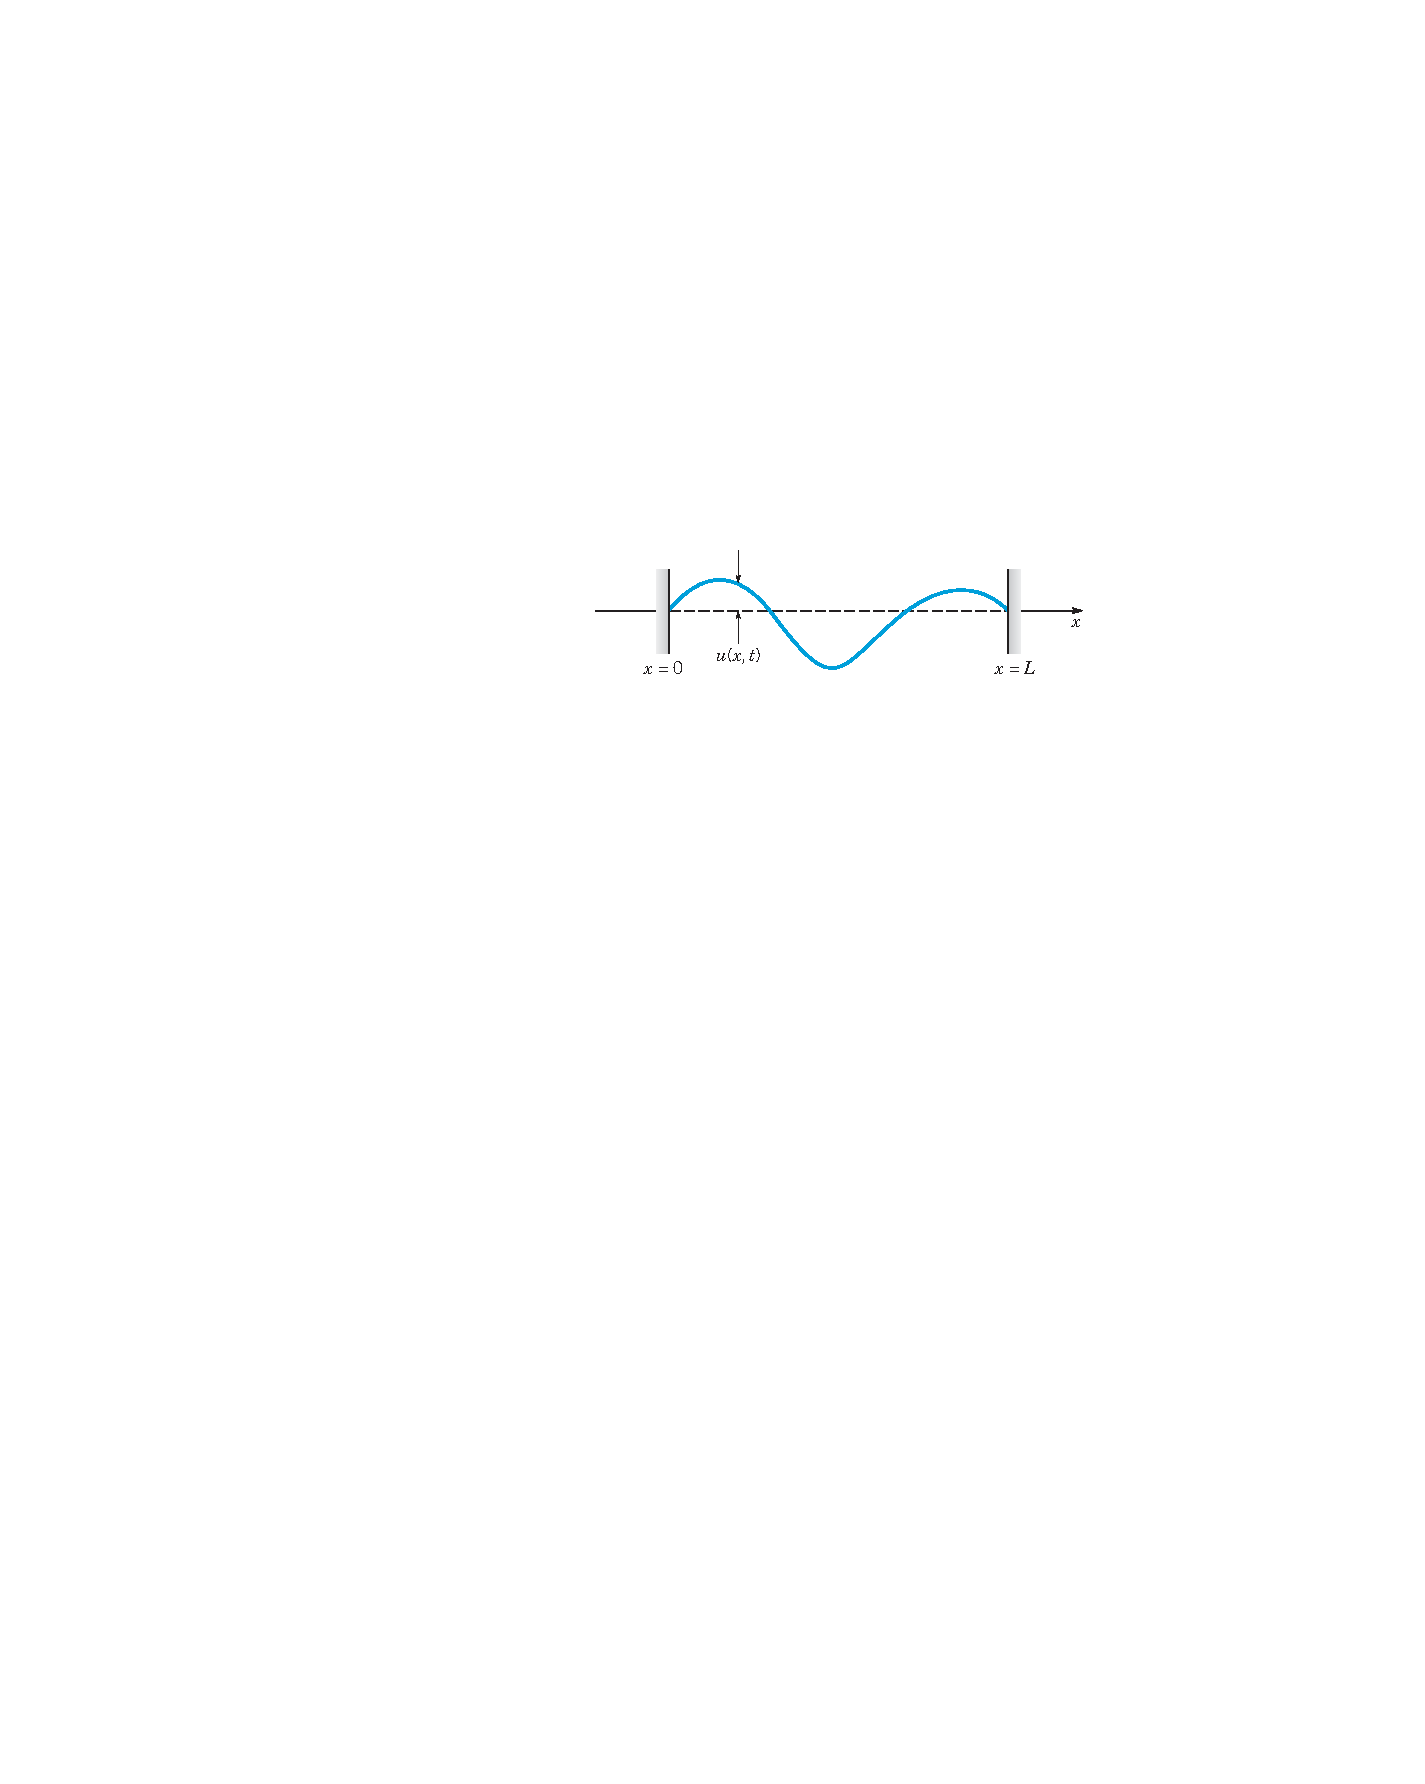
\includegraphics[width=0.7\textwidth]{WaveString.pdf}
	\caption{A vibrating string \cite[Figure 10.7.1]{boyce}.}
	\label{fig:wavestring}
\end{figure}

As before, we use separation of variables, writing
\begin{align*}
	u(x,t) &= X(x) T(t) \\
	\implies XT'' &= a^2 X''T \\
	\implies \frac{1}{a^2} \frac{T''}{T} &= \frac{X''}{X} = \lambda,
\end{align*}
where $\lambda$ is the separation constant.

We first solve the boundary value problem
\[
X'' = \lambda X, \quad X(0) = X(L) = 0.
\]
As was the case when this ODE appeared while solving the heat equation, we find that the eigenvalues are
\[
\lambda_n = -\frac{n^2\pi^2}{L^2},
\]
and the corresponding eigenfunctions are
\[
X_n(x) = \sin\left(\frac{n\pi x}{L}\right), \quad n = 1, 2, \dots.
\]

Now we solve the second ODE:
\[
T_n'' - a^2\lambda T_n = 0 \implies T_n'' + \frac{n^2\pi^2a^2}{L^2}T_n = 0.
\]
Since $\frac{n^2\pi^2a^2}{L^2} > 0$, we have solutions of the usual form:
\[
T_n(t) = a_n \cos\left(\frac{n\pi at}{L}\right) + b_n \sin\left(\frac{n\pi at}{L}\right).
\]

Therefore we have the following elementary solutions
\[
u_n(x,t) = X_n T_n(t) = \left(a_n \cos\left(\frac{n\pi at}{L}\right) + b_n \sin\left(\frac{n\pi at}{L}\right)\right) \sin\left(\frac{n\pi x}{L}\right), 
\]
and a general solution given by
\begin{equation}
	u(x,t) = \sum_{n=1}^{\infty} \left(c_n \cos\left(\frac{n\pi at}{L}\right) + d_n \sin\left(\frac{n\pi at}{L}\right)\right) \sin\left(\frac{n\pi x}{L}\right).
\end{equation}

Now we apply the first of the initial conditions
\[
u(x,0) = \sum_{n=1}^{\infty} c_n \sin\left(\frac{n\pi x}{L}\right) = f(x).
\]
This is nothing but the Fourier series for $f(x)$, with $f(x)$ being an odd function. Therefore, we apply the version of the Euler-Fourier equations found in \Cref{sec:evenoddfourier} to find that
\begin{equation}
	c_n = \frac{2}{L} \int_0^L f(x) \sin\left(\frac{n\pi x}{L}\right).
\end{equation}

Finally, using the second initial condition
\begin{align}
	\p_t u(x,0) &= \sum_{n=1}^{\infty}\frac{n\pi a}{L} d_n \sin\left(\frac{n\pi x}{L}\right) = g(x) \nonumber \\
	\implies \frac{n\pi a}{L} d_n &= \frac{2}{L} \int_0^L g(x) \sin\left(\frac{n\pi x}{L}\right) \nonumber \\
	d_n &= \frac{2}{n\pi a} \int_0^L g(x) \sin\left(\frac{n\pi x}{L}\right).
\end{align}

\begin{eg}\label{eg:waveeqn}
	We consider the case with initial condition $\p_t u = 0$ at $t=0$.
	
	In the case that $u(x,0)$ is given by the tent, we have already calculated the coefficients in \Cref{eg:heateqn1}. Thus the solution is given by, 
	\[
	u(x,t) = \sum_{k=0}^{\infty} \frac{8}{((2k+1)\pi)^2} (-1)^k \sin\left((2k+1)\pi x\right)\cos\left((2k+1)\pi t\right).
	\]
	This solution is shown in \Cref{fig:heateqneg1} for a few select values of $t$.
\end{eg}

\begin{figure}[!ht]
	\centering
	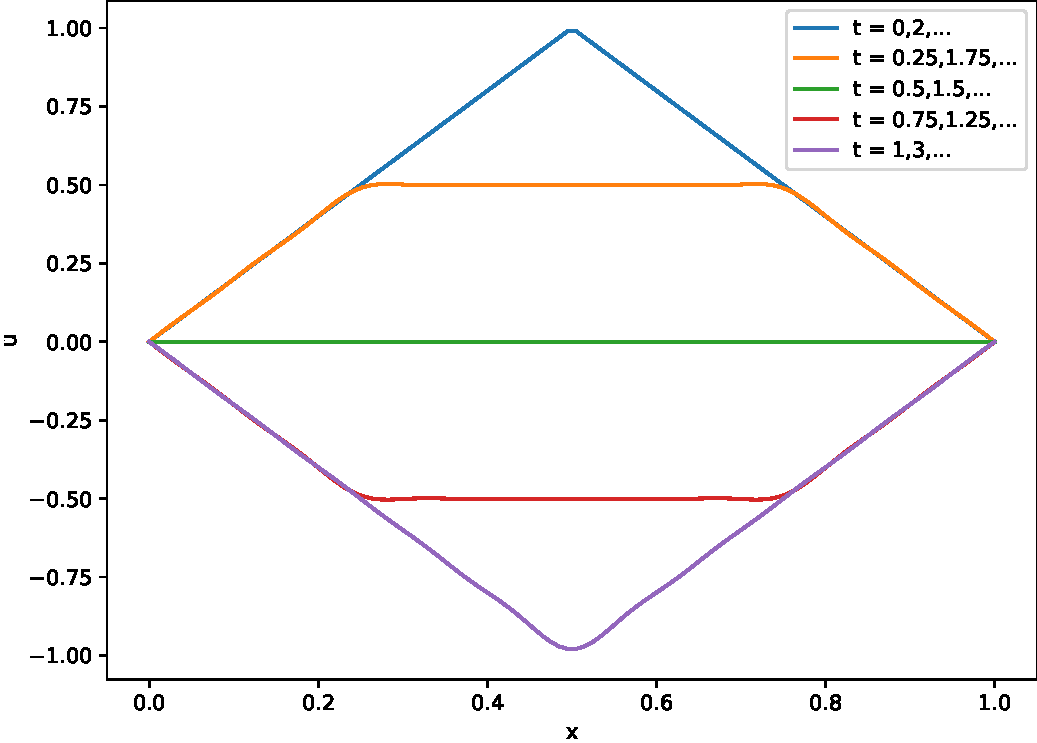
\includegraphics[width=0.7\textwidth]{WaveEqn.pdf}
	\caption{Solution of the heat equation given the initial conditions in \Cref{eg:waveeqn}.}
	\label{fig:waveeqn}
\end{figure}

\begin{eg}
	Let's see how we can interpret the solution of the wave equation when there is no initial velocity ($g(x) = 0$). This means that $d_n = 0$ for all $n$ so the solution is
	\[
	u(x,t) = \sum_{n=1}^{\infty} c_n \cos\left(\frac{n\pi at}{L}\right) \sin\left(\frac{n\pi x}{L}\right).
	\]
	The frequency of the cosine wave will be $f_n = \frac{1}{T_n} = \frac{n\pi a}{2L}$, where $T_n$ is the period of the wave. This suggests that we can decompose the overall solution as the sum of individual waves with period $\frac12$, $1$, $\frac32$, etc. as illustrated in \Cref{fig:harmonics}. These waves are called the fundamental modes of vibration or, in music, they are called the fundamental tone (or first harmonic), second harmonic, and so on.
\end{eg}

\begin{figure}[!ht]
	\centering
	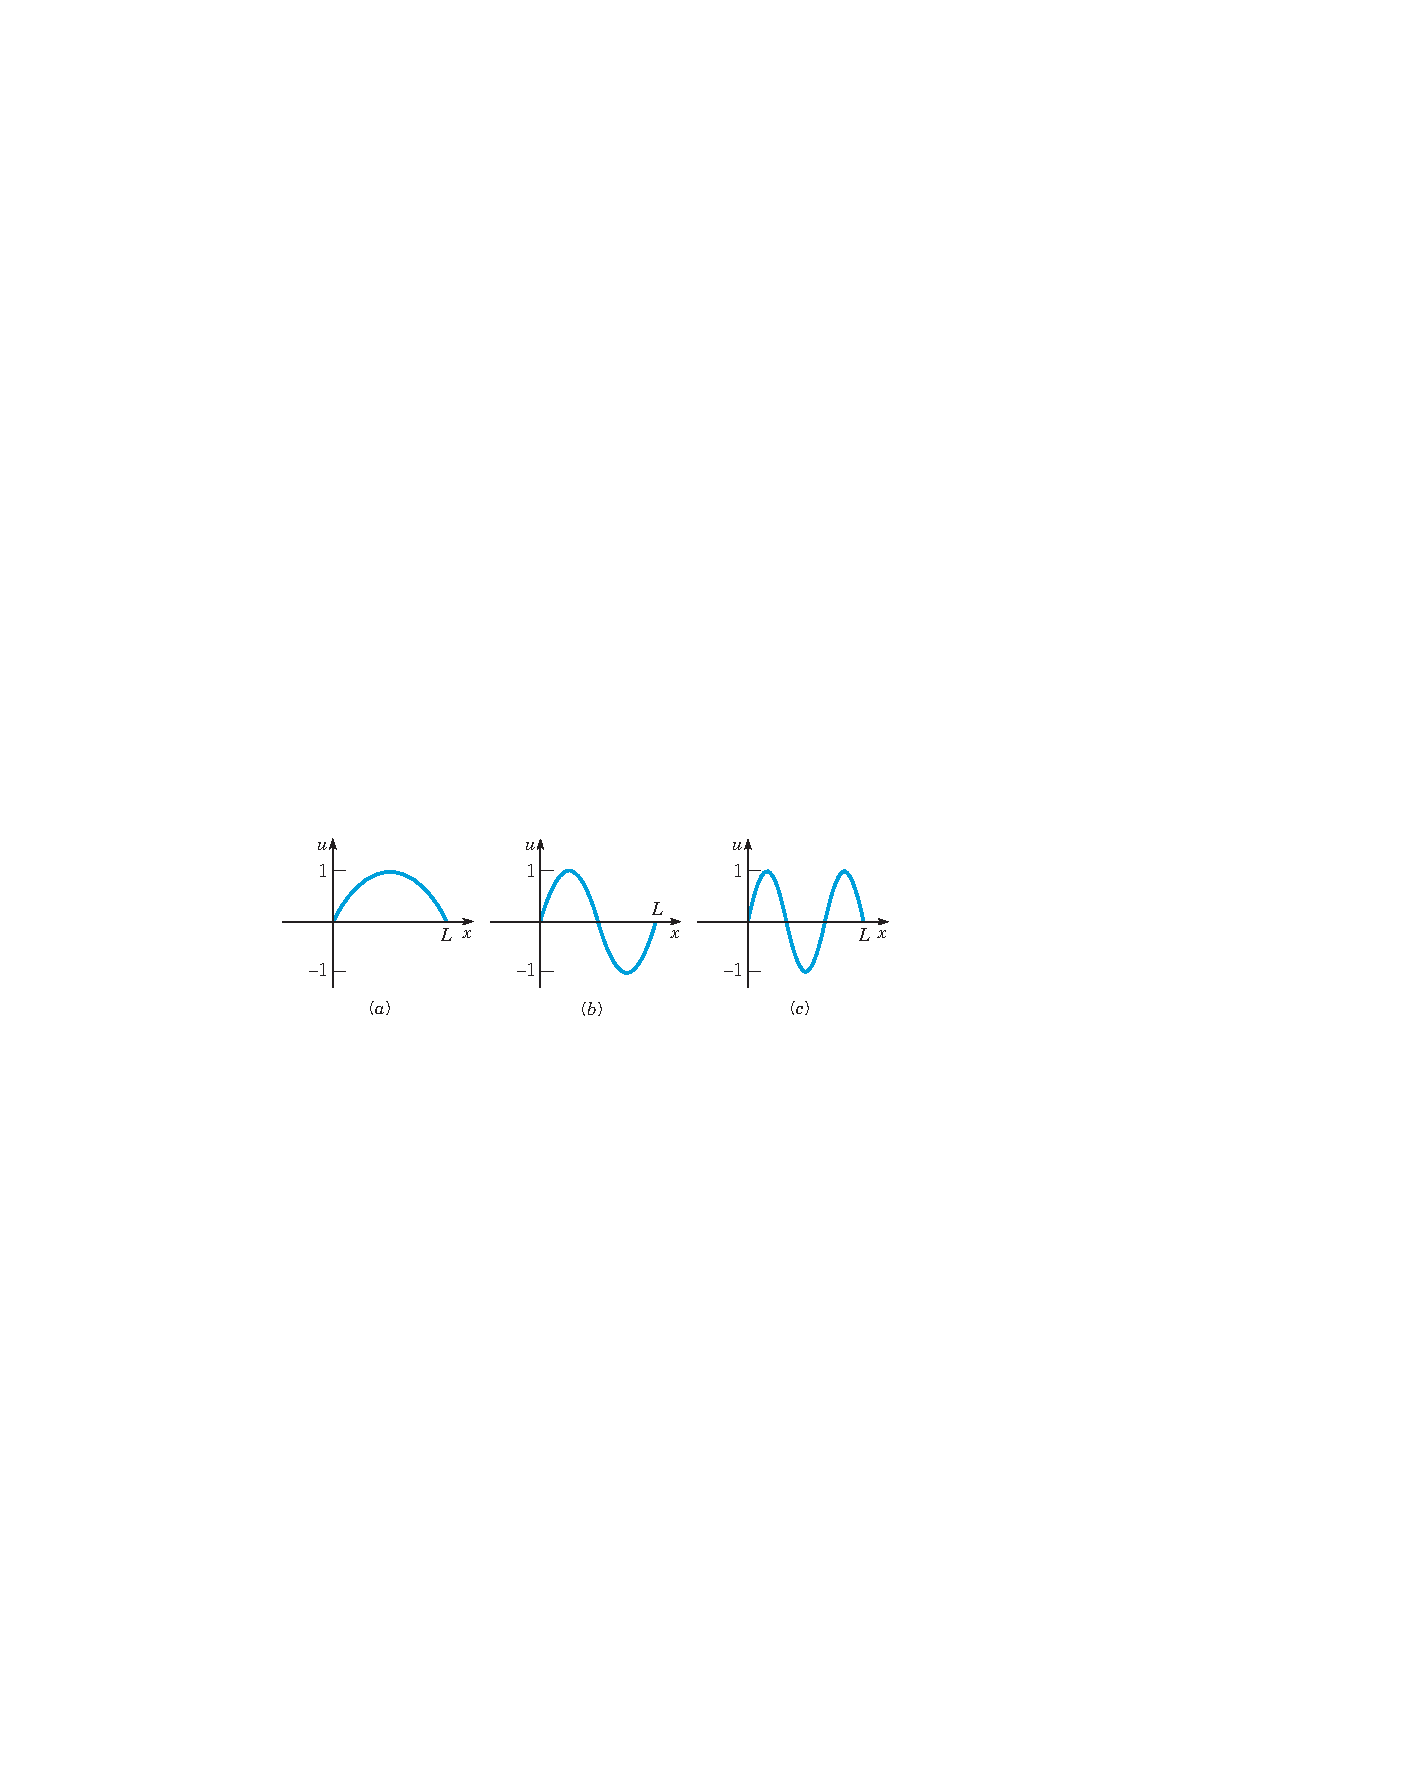
\includegraphics[width=0.7\textwidth]{Harmonics.pdf}
	\caption{First three harmonics for vibration in an elastic string, with frequencies (a) $\frac{\pi a}{L}$, (b) $\frac{2\pi a}{L}$, and (c) $\frac{3\pi a}{L}$ \cite[Figure 10.7.3]{boyce}.} 
	\label{fig:harmonics}
\end{figure}

\subsection{Laplace's Equation}

Laplace's equation is given by
\begin{equation}
	\nabla^2u = \p_{xx}u + \p_{yy}u = 0.
\end{equation}

This equation is time-independent and is widely used in physics describing situations of equilibrium, or those that do not depend explicitly on time, such as modelling the shape of soap bubbles or dispersion of heat in a steady state. Since the equation is not dependent on time, there are no initial conditions; only boundary conditions.

We will solve Laplace's equation on two domains: on a rectangle and on a circle.

\begin{enumerate}
	\item \textbf{Laplace's equation on a rectangle.}
	
	We solve
	\[
	\p_{xx}u + \p_{yy}u = 0 \quad \text{in} \quad 0 \leq x \leq a, \,\, 0 \leq y \leq b
	\]
	with the following boundary conditions
	\[
	u(x,0) = u(x,b) = u(0,y) = 0
	\]
	\[
	u(a,y) = f(y).
	\]
	As usual, we use separation of variables:
	\begin{align*}
		u(x,y) &= X(x)Y(y) \\
		\implies 0 &= X''Y + XY''\\
		\implies \frac{X''}{X} &= -\frac{Y''}{Y} = \lambda,
	\end{align*}
	where $\lambda$ is the usual separation constant.
	
	Based on the boundary conditions, it is easier to first solve
	\[
	Y'' = -\lambda Y, \quad Y(0) = Y(b) = 0.
	\]
	This is a boundary value problem we've solved before, with the following eigenvalues and eigenfunctions:\footnote{Note that the coefficient of $Y$ has the opposite sign to the previous examples, so now there is a non-trivial solution only if $\lambda>0$ i.e. $-\lambda<0$.}
	\[
	\lambda_n = -\frac{n^2\pi^2}{b^2}, \quad Y_n(y) = \sin\left(\frac{n\pi y}{b}\right).
	\]
	Now we solve the second equation
	\[
	X'' = \lambda X \implies X'' - \frac{n^2\pi^2}{b^2}X = 0, \quad X(0)=0.
	\]
	Same as before, we find that the solutions are of the form
	\[
	X(x) = A\cosh\left(\frac{n\pi x}{b}\right) + B\sinh\left(\frac{n\pi x}{b}\right).
	\]
	Applying the initial condition, we find $X(0) = 0 = A$, therefore the final eigenfunction is given by
	\[
	X_n(x) = \sinh\left(\frac{n\pi x}{b}\right).
	\]
	In sum, we have elementary solutions of the form
	\[
	u_n(x,t) = X_n(x) Y_n(y) = \sinh\left(\frac{n\pi x}{b}\right) \sin\left(\frac{n\pi y}{b}\right),
	\]
	and using superposition to find the general solution yields
	\begin{equation}
		u(x,y) = \sum_{n=1}^{\infty} c_n \sinh\left(\frac{n\pi x}{b}\right) \sin\left(\frac{n\pi y}{b}\right).
	\end{equation}
	All that remains is to use the final boundary condition:
	\[
	u(a,y) = f(y) = \sum_{n=1}^{\infty} c_n \sinh\left(\frac{n\pi a}{b}\right) \sin\left(\frac{n\pi y}{b}\right).
	\]
	This is recognisable as the Fourier series for an odd function or odd extension, where $c_n \sinh\left(\frac{n\pi a}{b}\right)$ are the Fourier coefficients. Therefore applying the Euler-Fourier formulas, we get
	\begin{align}
		c_n \sinh\left(\frac{n\pi a}{b}\right) &= \frac{2}{b} \int_0^b f(y)\sin\left(\frac{n\pi y}{b}\right)dy \nonumber \\
		c_n &= \frac{2}{b\sinh\left(\frac{n\pi a}{b}\right)} \int_0^b f(y)\sin\left(\frac{n\pi y}{b}\right)dy.
	\end{align}
	
	\begin{eg}\label{eg:laplacerect}
		We solve Laplace's equation on the rectangle $0 \leq x \leq 1$, $0 \leq y \leq 1$, where the boundary condition has $f(y)$ being the tent function
		\[
		f(y) = \begin{cases} 2y & \text{if } y \leq \frac12 \\ 2(1-y) & \text{if } y>\frac12 \end{cases}.
		\]
		In order to calculate $c_n$, we need to evaluate
		\begin{align*}
			\int_0^b f(y)\sin\left(\frac{n\pi y}{b}\right)dy &= \int_0^1 f(y)\sin(n\pi y) \,dy \\
			&= \int_0^{1/2} 2y\sin(n\pi y) \,dy + \int_{1/2}^1 2(1-y)\sin(n\pi y) \,dy.
		\end{align*}
		Evaluating the first integral
		\begin{align*}
			\int_0^{1/2} 2y\sin(n\pi y) \,dy &= \left[ -\frac{2}{n\pi}y\cos(n\pi y)\right]_0^{1/2} + \int_0^{1/2} \frac{2}{n\pi} \cos(n\pi y) \,dy \\
			&= \frac{2}{n\pi}\left[-y\cos(n\pi y)\right]_0^{1/2} + \frac{2}{n^2\pi^2}\left[\sin(n\pi y)\right]_0^{1/2} \\
			&= -\frac{1}{n\pi} \cos\left(\frac{n\pi}{2}\right) + \frac{2}{n^2\pi^2} \sin\left(\frac{n\pi}{2}\right).
		\end{align*}
		And now turning to the second integral
		\begin{align*}
			&\int_{1/2}^1 2(1-y)\sin(n\pi y) \,dy \\
			&= \int_{1/2}^1 2\sin(n\pi y) \,dy - \int_{1/2}^1 2y\sin(n\pi y) \,dy \\
			&= 2\left(\left[-\frac{1}{n\pi}\cos(n\pi y)\right]_{1/2}^1 - \left( \left[-\frac{1}{n\pi}y\cos(n\pi y)\right]_{1/2}^1 + \int_{1/2}^1 \frac{1}{n\pi}\cos(n\pi y) \,dy \right)\right) \\
			&= 2\left(\frac{\cos(n\pi/2)}{n\pi} -\cancel{\frac{\cos(n\pi)}{n\pi}} + \cancel{\frac{\cos(n\pi)}{n\pi}} - \frac{\cos(n\pi/2)}{2n\pi} + \cancelto{0}{\frac{\sin(n\pi)}{n^2\pi^2}} + \frac{\sin(n\pi/2)}{n^2\pi^2}\right) \\
			&= \frac{1}{n\pi} \cos\left(\frac{n\pi}{2}\right) + \frac{2}{n^2\pi^2} \sin\left(\frac{n\pi}{2}\right).
		\end{align*}
		Summing these two expressions, the original integral is
		\begin{align*}
			\int_0^1 f(y)\sin(n\pi y) \,dy &= \frac{4}{n^2\pi^2} \sin\left(\frac{n\pi}{2}\right) \\
			\implies c_n &= \frac{8}{n^2\pi^2\sinh(n\pi)} \sin\left(\frac{n\pi}{2}\right)
		\end{align*}
		We know $\sin(n\pi/2)$ is non-zero only for odd $n$, oscillating between 1 and -1. Therefore, the final solution can be written as 
		\[
		u(x,y) = 8\sum_{n=0}^{\infty} \frac{(-1)^n}{(2n+1)^2\pi^2 \sinh\left((2n+1)\pi\right)} \sinh\left((2n+1)\pi x\right) \sin\left((2n+1)\pi y\right),
		\] 
		which is shown in \Cref{fig:laplacerect}
	\end{eg}
	
	\begin{figure}[!ht]
		\centering
		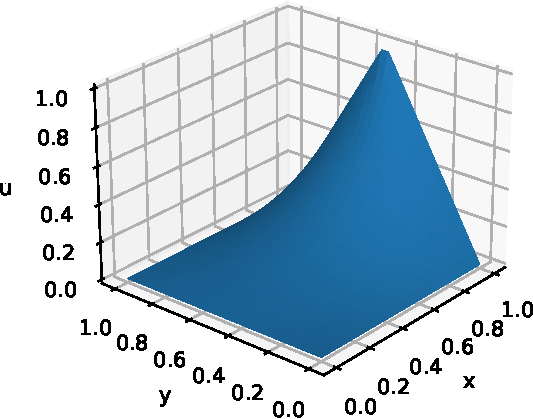
\includegraphics[width=0.7\textwidth]{LaplaceRect.pdf}
		\caption{The solution of Laplace's equation with the boundary conditions $u(x,0) = u(x,b) = u(0,y) = 0$ and $u(a,y) = f(y)$, where $f(y)$ is the tent function. Intuitively, this may be thought of as the shape a soap bubble would take given these boundary conditions.}
		\label{fig:laplacerect}
	\end{figure}
	
	\item \textbf{Laplace's equation on a disc.}
	
	In this case, we solve
	\[
	u_{xx} + u_{yy} = 0, \quad u(r=a, \theta) = f(\theta),
	\]
	where we see that the boundary conditions are given in polar coordinates. To proceed, we need to find the Laplacian in polar coordinates, which is\footnote{For a derivation of this, see \url{https://www.math.ucdavis.edu/~saito/courses/21C.w11/polar-lap.pdf}.}
	\begin{align*}
		\frac{1}{r}(r u_r)_r + \frac{1}{r^2}u_{\theta\theta} &= 0 \\
		\frac{\p^2u}{\p r^2} + \frac{1}{r}\frac{\p u}{\p r} + \frac{1}{r^2}\frac{\p^2u}{\p\theta^2} &= 0.
	\end{align*}
	
	Now to solve this equation, we use the usual method of separation of variables
	\begin{align*}
		u(r, \theta) &= R(r)\Theta(\theta) \\
		0 &= \frac{1}{r}(r R_r)_r\Theta + \frac{1}{r^2}R \Theta_{\theta\theta} \\
		\frac{r(rR')'}{R} &= -\frac{\Theta''}{\Theta} = \lambda,
	\end{align*}
	where in the final line we use $R'$ and $\Theta'$ to denote differentiation with respect to the relevant independent variable since $R$ and $\Theta$ are functions of one variable.
	
	Now, we shall solve $\Theta'' = -\lambda\Theta$, using the condition that $\Theta$ must be $2\pi$-periodic in $\theta$. As usual, we have three cases:
	\begin{itemize}
		\item Case 1: $\lambda = \mu^2 > 0$. Then the solution is
		\[
		\Theta = A\cos(\mu\theta) + B\sin(\mu\theta),
		\]
		where $\mu = n = 1, 2, \dots$ for $2\pi$-periodic solutions.
		\item Case 2: $\lambda=0$. The solution is
		\[
		\Theta = A\theta + B,
		\]
		which implies that $\Theta$ is constant for it to be periodic.
		\item Case 3: $\lambda = -\mu^2 < 0$. The solution is
		\[
		\Theta = A\cosh(\mu\theta) + B\sinh(\mu\theta),
		\]
		which is never periodic, thus there are no solutions.
	\end{itemize}
	
	So overall, the eigenvalues are
	\[
	\lambda_0 = 0 \quad \text{and} \quad \lambda_n = n^2,
	\]
	and the corresponding eigenfunctions are
	\[
	\Theta_0(\theta) = 1 \quad \text{and} \quad \Theta_n(\theta) = c_n\cos(n\theta) + d_n\sin(n\theta).
	\]
	Alternatively, we may split the eigenfunction $\Theta_n$ into two separate functions:
	\[
	\Theta_n(\theta) = \cos(n\theta) \quad \text{and} \quad \widetilde{\Theta}_n(\theta) = \sin(n\theta).
	\]
	
	Now, we turn to solving the second equation, $\frac{r(rR')'}{R} = \lambda \iff r(rR')' = n^2R$. We split this into two cases:
	\begin{itemize}
		\item Case 1: $n=0$. In this case, the equation becomes
		\[
		(rR')' = 0 \implies rR' = A \implies R = \cancelto{0}{A\log r} + B
		\]
		since the solution must be bounded (so we cannot have $\log r$ being unbounded as $r \to 0$). Therefore the solution in this case is constant.
		\item Case 2: $n = 1, 2, \dots$. The equation becomes
		\[
		r^2R'' + rR' - n^2R = 0,
		\]
		which is an Euler equation. To solve such equations, we try $R(r) = r^{\alpha}$, yielding
		\begin{align*}
			\alpha(\alpha-1)r^{\alpha} + \alpha r^{\alpha} - n^2r^{\alpha} &= 0 \\
			\alpha^2 &= n^2 \\
			\alpha &= \pm n.
		\end{align*}
		Therefore
		\[
		R(r) = Ar^n + \cancelto{0}{Br^{-n}},
		\]
		where we cancel $r^{-n}$ by setting $B=0$ so that the solution is bounded as $r\to 0$.
	\end{itemize}
	Putting all this together, we have the following elementary solutions
	\[
	u_0(r,\theta) = 1, \quad u_n(r,\theta) = r^n\cos(n\theta), \quad \widetilde{u}_n(r,\theta) = r^n\sin(n\theta),
	\]
	and using superposition to find the general solution yields
	\begin{equation}\label{eq:laprectgensol}
		u(r,\theta) = a_0 + \sum_{n=1}^{\infty} r^n\left(a_n\cos(n\theta) + b_n\sin(n\theta)\right).
	\end{equation}
	
	To complete the solution, we use the given boundary condition 
	\[
	u(a, \theta) = \frac{a_0}{2} + \sum_{n=1}^{\infty} a_na^n \cos(n\theta) + b_na^n \sin(n\theta) = f(\theta).
	\]
	This is nothing but a Fourier series with $2L = 2\pi$ and Fourier coefficients $a_na^n$ and $b_na^n$.\footnote{Observe that we have replaced $a_0$ with $\frac{a_0}{2}$ to match the Fourier series form.} By the usual method of using the Euler-Fourier equations, we find that
	\begin{align}
		\label{eq:lapdisccoeff1}
		a_n &= \frac{1}{a^n\pi} \int_{-\pi}^{\pi} f(\theta) \cos(n\theta) \,d\theta \\
		\label{eq:lapdisccoeff2}
		b_n &= \frac{1}{a^n\pi} \int_{-\pi}^{\pi} f(\theta) \sin(n\theta) \,d\theta \\
		a_0 &= \frac{1}{\pi} \int_{-\pi}^{\pi} f(\theta) \,d\theta
	\end{align}
	
	\begin{remark}
		If $f(\theta)$ is an odd function, then the integrand $f(\theta) \cos(n\theta)$ in \Cref{eq:lapdisccoeff1} is odd, so $a_n=0$ and the terms in $\cos(n\theta)$ vanish. Similarly, if $f(\theta)$ is an even function, $f(\theta) \sin(n\theta)$ in \Cref{eq:lapdisccoeff2} is odd and $b_n=0$ for all $n$.
	\end{remark}
	
	\begin{remark}
		The more general solution for Laplace's equation on the annulus $r_1 \leq r \leq r_2$, $-\pi \leq \theta \leq \pi$ is
		\begin{equation}
			u(r,\theta) = \frac{a_0}{2} + \frac{\hat{a}_0}{2}\log{r} + \sum_{n=1}^{\infty} \left(a_nr^n + \hat{a}_nr^{-n}\right)\cos(n\theta) + \sum_{n=1}^{\infty} \left(b_nr^n + \hat{b}_nr^{-n}\right)\sin(n\theta)
		\end{equation}
		for arbitrary real constants $a_n$, $\hat{a}_n$, $b_n$, and $\hat{b}_n$. Note that this becomes the solution in \Cref{eq:laprectgensol} when we take $r_1=0$ and impose $\hat{a}_n = \hat{b}_n = 0$ for all $n$ so the solution is bounded.
	\end{remark}
	
	\begin{eg}
		We solve Laplace's equation on the disc $r \leq 1$ with the Dirichlet boundary conditions
		\[
		u(1, \theta) = \begin{cases} 1 & \text{if } -\frac{\pi}{2} < \theta < \frac{\pi}{2} \\ 0 & \text{otherwise} \end{cases}.
		\]
		Solving for $a_n$ and $b_n$ is much easier than in \Cref{eg:laplacerect}, therefore this working is left as an exercise. We note only that solution is 
		\[
		u(r,\theta) = \sum_{n=1}^{\infty} \frac{2}{n\pi}\sin\left(\frac{n\pi}{2}\right) r^n \cos(n\theta),
		\] 
		which is shown in \Cref{fig:laplacecircle}.
	\end{eg}
	
	\begin{figure}[!ht]
		\centering
		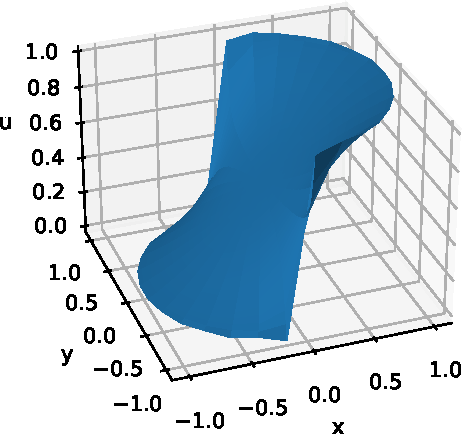
\includegraphics[width=0.7\textwidth]{LaplaceCircle.pdf}
		\caption{The solution of Laplace's equation on a disc with Dirichlet boundary conditions.}
		\label{fig:laplacecircle}
	\end{figure}
\end{enumerate}
\section{Sturm-Liouville Theory}\label{sec:slmain}

Sturm-Liouville Theory is the theory of second-order boundary value eigenproblems of the form
\begin{equation}
	-\left(p(x)y'\right)' + q(x)y = \lambda r(x)y, \quad y(0)=y(1)=0.
\end{equation}

\subsection{Motivation}

Two ideas motivate Sturm-Liouville theory.

\begin{enumerate}
	\item \textbf{Eigenvalues of symmetric matrices.}
	
	The eigenvalues and eigenvectors of a symmetric matrix may be represented as follows:
	\begin{equation}\label{eq:sleigs}
		A\xib_n = \lambda_n\xib_n, \quad A^T = A.
	\end{equation}
	The following properties are equivalent to the condition of a matrix being symmetric:
	\begin{itemize}
		\item $\bm{u} \cdot A\bm{v} = \bm{v} \cdot A\bm{u}$, $\forall \bm{u},\bm{v}$,
		\item $\xib_m\cdot\xib_n = 0$ for $m \neq n$.
	\end{itemize}
	We can see that the second property follows from the first by taking the dot product of $\xib_m$ and $\xib_n$ (for $m\neq n$) with \Cref{eq:sleigs},
	\begin{align*}
		\xib_m\cdot A\xib_n &= \xib_m\cdot(\lambda_n\xib_n) = \lambda_n \xib_m\cdot\xib_n \\
		\xib_n\cdot A\xib_m &= \lambda_m \xib_n\cdot\xib_m.
	\end{align*}
	Taking the difference of these two equations yields
	\[
	\xib_m\cdot A\xib_n - \xib_n\cdot A\xib_m = (\lambda_n - \lambda_m)\xib_n\cdot\xib_m = 0,
	\]
	since $\xib_m\cdot A\xib_n = \xib_n\cdot A\xib_m$ from the first property. Therefore if $\lambda_m \neq \lambda_n$, we can conclude that $\xib_m\cdot\xib_n = 0$ for $m \neq n$.
	
	\item \textbf{Fourier series with eigenfunctions} $X_n(x) = \sin\left(\frac{n\pi x}{L}\right)$.
	
	From the definition of eigenvalues and eigenfunctions, we know that\footnote{In this equation, the $L$ in $LX_n$ represents the linear map defined in \Cref{eg:linearmap}, while $L$ in $X_n(L)$ is a scalar related to the period of the function. Generally, common sense should be enough to determine which is which.}
	\[
	LX_n = X_n'' = \lambda_n X_n, \quad X_n(0) = X_n(L) = 0.
	\]
	We know that these functions $X_n$ are orthogonal (where orthogonality was defined in \Cref{eq:innerprod}), therefore $(X_m, X_n) = 0$ for $m \neq n$. From the definition of orthogonality, we can see that
	\begin{align*}
		(X_m, LX_n) &= \lambda_n (X_m, X_n) \\
		(X_n, LX_m) &= \lambda_m (X_n, X_m).
	\end{align*}
	Therefore
	\begin{align*}
		(\lambda_n - \lambda_m)(X_m, X_n) &= (X_m, LX_n) - (X_n, LX_m) \\
		&= \int_0^L X_mX_n'' - X_m''X_n\,dx \\
		&= \cancelto{0}{\left[X_mX_n'\right]_0^L} - \cancel{\int_0^LX_m'X_n' \,dx} - \cancelto{0}{\left[X_m'X_n\right]_0^L} + \cancel{\int_0^L X_m'X_n' \,dx} \\
		&= 0
	\end{align*}
	Since $(\lambda_n - \lambda_m)(X_m, X_n) = 0$, we find that $(X_m,X_n) = 0$ when $\lambda_m \neq \lambda_n$ and $m \neq n$.
	
	Therefore, we have established orthogonality of the functions $X_n(x) = \sin\left(\frac{n\pi x}{L}\right)$ without using trigonometry: the only fact we needed was that these sine functions satisfy the eigenvalue problem.
\end{enumerate}

Thus, we have learned that if $L = \frac{d^2}{dx^2}$, then
\begin{equation}
	(u, Lv) - (v, Lu) = 0, \quad \forall u,v,
\end{equation}
where
\[
(u,v) = \int_0^1 u(x)v^*(x) \,dx
\]
(compare this to \Cref{eq:innerprodcomplex}.) This is called \textbf{Lagrange's Identity}.

Operators that satisfy this property are equivalent to symmetric matrices and are called self-adjoint operators. Thus, essentially everything we know about symmetric matrices (e.g. orthogonal eigenvectors, real eigenvalues, etc.) will hold when working with these operators.

\subsection{Sturm-Liouville Eigenvalue Problems}

\begin{definition}
	The eigenvalue ODE equation
	\begin{equation}\label{eq:sturmliou}
		Ly = -\left(p(x)y'\right)' + q(x)y = \lambda r(x)y, \quad 0 \leq x \leq 1,
	\end{equation}
	subject to the boundary conditions
	\begin{equation}\label{eq:sturmliouconds}
		\begin{alignedat}{1}
			a_1y(0) + a_2y'(0) &= 0 \\
			b_1y(1) + b_2y'(1) &= 0.
		\end{alignedat}
	\end{equation}
	defines a (regular) \textbf{Sturm-Liouville boundary problem}, where the functions $p$, $q$, $r$, and $p'$ are continuous and $p$ and $r$ are strictly positive.
\end{definition}

We will make use of Lagrange's Identity which was stated in the previous section, i.e. that
\[
(u, Lv) = (v, Lu).
\]
We can prove this without too much trouble for the problems of the form in \Cref{eq:sturmliou}.

\begin{proof}
	\begin{align*}
		(u, Lv) &= \int_0^1 u\left(-(pv^{*\prime})' + qv^*\right) \,dx \\
		&= \left[-puv^{*\prime}\right]_0^1 + \int_0^1 pu'v^{*\prime} + quv \,dx \\
		&= \left[-puv^{*\prime}\right]_0^1 + \left[pu'v^*\right]_0^1 + \int_0^1 (-(pu')' + qu)v^* \,dx \\
		&= \left[pu'v^*-puv^{*\prime}\right]_0^1 + \int_0^1 Luv^* \,dx \\
		&= p(1)\left(u'(1)v^*(1) - u(1)v^{*\prime}(1)\right) - p(0)\left(u'(0)v^*(0) - u(0)v^{*\prime}(0)\right) + (Lu, v).
	\end{align*}
	But from \Cref{eq:sturmliouconds},
	\[
	u'(1) = -\frac{a_2}{a_1}u(1) \quad\text{and}\quad v^{*\prime}(1) = -\frac{a_2}{a_1}v^*(1)
	\]
	therefore
	\begin{align*}
		u'(1)v^*(1) - u(1)v^{*\prime}(1) &= 0 \\
		u'(0)v^*(0) - u(0)v^{*\prime}(0) &= 0
	\end{align*}
	and so we have proved that
	\[
	(u, Lv) = (Lu, v) = (v, Lu).
	\]
\end{proof}

Properties:
\begin{enumerate}
	\item The eigenvalues are real, $\lambda_n \in \R$.
	\item The eigenfunctions are orthogonal:
	\[
	\langle \phi_m, \phi_n \rangle = \int_0^1 \phi_m(x)\phi_n^*(x)r(x) \,dx = (\phi_m, r\phi_n) = 0 \quad \text{if } \lambda_m \neq \lambda_n.
	\]
\end{enumerate}

\begin{proof}\leavevmode
	\begin{enumerate}
		\item We apply Lagrange's Identity to $u = \phi_n$ and $u = \phi_n$, noting that we have $L \phi_n = \lambda_n r\phi_n$ since we are dealing with problems of the form in \Cref{eq:sturmliou}. Then
		\begin{align*}
			&(L\phi_n, \phi_n) = (\phi_n, L\phi_n) \\
			\implies &(\lambda_n r\phi_n, \phi_n) = (\phi_n, \lambda_n r\phi_n) \\
			\implies &\lambda_n(r\phi_n, \phi_n) = \lambda_n^*(\phi_n, r\phi_n) \\
			\implies &(\lambda_n - \lambda_n^*) \underbrace{\int_0^1 r |\phi_n|^2 \,dx}_{\neq 0} = 0 \\
			\implies &\lambda_n = \lambda_n^* \text{ i.e. } \lambda_n \in \R. 
			\intertext{\item We apply Lagrange's identity to $u = \phi_n$, $v = \phi_m$. Then}
			&(L\phi_n, \phi_m) = (\phi_n, L\phi_m) \\
			\implies &(\lambda_n r\phi_n, \phi_m) = (\phi_n, \lambda_m r\phi_m) \\
			\implies &(\lambda_n - \lambda_m)(r\phi_n, \phi_m) = 0 \tag{$\lambda_n = \lambda_n^*$} \\
			\implies &(r\phi_n, \phi_m) = 0 \text{ for } \lambda_n \neq \lambda_m.
		\end{align*}
		Therefore $\langle \phi_m, \phi_n \rangle = 0$ also.
	\end{enumerate}
\end{proof}

\begin{remark}
	As the eigenvalues are real, so too are the eigenfunctions.
\end{remark}

\begin{theorem}
	The eigenvalues form an ordered sequence
	\[
	\lambda_1 < \lambda_2 < \cdots < \lambda_n \to \infty,
	\]
	and there is a unique eigenfunction for each $\lambda_n$.
\end{theorem}

\begin{proof}
	Me providing a proof that everyone can use is basically socialism. Pull yourself up by your bootstraps and create a proof yourself.
\end{proof}

\begin{eg}\label{eg:sl1}
	We solve the following Sturm-Liouville problem:
	\[
	-y'' = \lambda y, \quad\text{with}\quad y(0)=0,\,\, y(1) + y'(1) = 0.
	\]
	As is typical for solving this sort of problem, we split it into three cases depending on whether $\lambda$ is positive, negative, or zero:
	\begin{itemize}
		\item Case 1: $\lambda = \mu^2 > 0$. Then the solution is
		\[
		y(x) = A\cos(\mu x) + B\sin(\mu x)
		\]
		Applying the boundary conditions,
		\begin{align*}
			y(0) &= A = 0 \\
			y(1) + y'(1) &= B\sin\mu + \mu B\cos\mu = 0 \text{ where } \tan\mu = -\mu.
		\end{align*}
		This has infinitely many solutions (graph the functions to see this), therefore we have eigenvalues of the form $\lambda_n = \mu_n^2$ and eigenfunctions $Y_n(x) = \sin(\mu_n x) = \sin(\sqrt{\lambda_n}x)$ for $n \in \mathbb{N}$, where $\mu_n$ is the $n$th solution of the equation $\tan\mu = -\mu$.
		
		\item Case 2: $\lambda = 0$. The solution is
		\[
		y(x) = Ax + B,
		\]
		and applying the boundary conditions yields
		\begin{align*}
			y(0) &= B = 0 \\
			y(1) + y'(1) &= 2A = 0,
		\end{align*}
		hence we only have trivial solutions in this case.
		
		\item Case 3: $\lambda = -\mu^2 < 0$. The solution is
		\[
		y(x) = A\cosh(\mu x) + B\sinh(\mu x),
		\]
		and similar to Case 1, applying the boundary conditions yields the condition $\tanh\mu = -\mu$, which has no solutions except the trivial $\mu = 0$.
	\end{itemize}
	Therefore, the only solutions to this problem are those from Case 1.
\end{eg}

\subsubsection{Normalisation of Eigenfunctions}\label{sec:normaleigenfuncs}

In the previous example, we found that the eigenfunctions were such that
\[
\phi_n = k_n \sin(\sqrt{\lambda_n}x).
\]

What we can do is impose the condition $\langle \phi_n, \phi_n \rangle = 1$ to make these functions orthonormal as well as orthogonal. We can calculate the values of $k_n$ as follows:
\begin{align*}
	1 &= k_n^2 \int_0^1 \sin^2(\sqrt{\lambda_n} x) \,dx = \frac{k_n^2}{2} \int_0^1 1 - \cos(2\sqrt{\lambda_n}x) \,dx \\
	&= \frac{k_n^2}{2} \left(1 - \frac{\sin(2\sqrt{\lambda_n})}{2\sqrt{\lambda_n}}\right) = \frac{k_n^2}{2} \left(1 - \frac{2\sin\sqrt{\lambda_n}\cos\sqrt{\lambda_n}}{2\sqrt{\lambda_n}}\right) \\
	\intertext{From \Cref{eg:sl1}, we found that $\sin\mu + \mu\cos\mu = 0 \implies \frac{1}{\sqrt{\lambda_n}}\sin\sqrt{\lambda_n} = -\cos\sqrt{\lambda_n}$. Making this substitition yields}
	&= \frac{k_n^2}{2} (1 + \cos^2\sqrt{\lambda_n}) \\
	k_n &= \left(\frac{2}{1 + \cos^2\sqrt{\lambda_n}}\right)^{\frac12}.
\end{align*}

\subsection{Further Results on Sturm-Liouville Problems}

Eigenfunctions of Sturm-Liouville provide a complete basis in which to expand functions. We use this to solve some inhomogeneous boundary-value problems and some PDEs.
Sturm-Liouville problems are eigenvalue problems where 
\begin{equation}\label{eq6.2.1}
	L[\phi_n] = \lambda_n r(x) \phi
\end{equation}
\[
L[u] = -(pu')' + qu
\]

Note that $L[u]$ in the above equation is called the Sturm-Liouville Operator.

If we look at the boundary conditions for \Cref{eq6.2.1}, they must satisfy the Lagrange identity, i.e., if we have two functions $u, v$ which satisfy the same boundary conditions as $\phi_n$, then the inner products
\[
(Lu, v) = (u, Lv)
\]
The inner product:
\begin{align*}
	\langle \phi_m, \phi_n\rangle &= (\phi_m, r(x)\phi_n) \\
	&= \int_0^1 \phi_m(x) \phi_n(x) r(x) \,dx = \delta_{mn} = \begin{cases} 0 & \text{if } m \neq n \\ 1 & \text{if } m = n \end{cases}
\end{align*}

\subsubsection{Expanding Functions}\label{sec:slexpand}

We now want to expand any function in the basis made up of the eigenfunctions $\phi_n$:
\[
f(x) = \sum_{n=1}^{\infty}c_n \phi_n(x)
\]
So if the expansion holds, we can find $c_n$ by projecting $f$ on $\phi_m$
\begin{align*}
	\langle f, \phi_m\rangle &= \sum_{n=1}^{\infty} c_n \underbrace{\langle \phi_n, \phi_m\rangle}_{=\delta_{mn}} = c_m
\end{align*}
The formula
\[
c_m = \langle f, \phi_n\rangle
\]
is essentially a generalisation of the Euler-Fourier formulas, which gave the expansion for functions $\phi_n$ in terms of cosines and sines.

\begin{eg}\label{eg:slexpand}
	Expand the function $f(x) = x$ in the interval $0<x<1$ using the orthonormal set from \Cref{eg:sl1}:
	\[
		f(x) = x = \sum_{n=1}^{\infty} c_n \quad\text{with}\quad \phi_n = k_n \sin(\sqrt{\lambda_n} x).
	\]
	Using orthonormality, the unknown coefficients are fixed by
	\begin{align*}
		c_n &= k_n \int_0^1 x \sin(\sqrt{\lambda_n} x) \,dx \\
		&= k_n \left( \left[-\frac{x}{\sqrt{\lambda_n}}\cos(\sqrt{\lambda_n} x)\right]_0^1 + \int_0^1 \frac{1}{\sqrt{\lambda_n}} \cos(\sqrt{\lambda_n} x) \,dx \right) \\
		&= k_n\left( -\frac{1}{\sqrt{\lambda_n}}\cos\sqrt{\lambda_n} + \left[\frac{1}{\lambda_n} \sin(\sqrt{\lambda_n} x)\right]_0^1 \right) \\
		&= k_n\left( -\frac{1}{\sqrt{\lambda_n}}\cos\sqrt{\lambda_n} + \frac{1}{\lambda_n} \sin\sqrt{\lambda_n} \right)
		\intertext{Using the relation $\cos\sqrt{\lambda_n}= -\frac{1}{\sqrt{\lambda_n}}\sin\sqrt{\lambda_n}$ like in \Cref{sec:normaleigenfuncs}}
		&= k_n\left( \frac{1}{\lambda_n}\sin\sqrt{\lambda_n} + \frac{1}{\lambda_n} \sin\sqrt{\lambda_n} \right) \\
		&= k_n \frac{2\sin\sqrt{\lambda_n}}{\lambda_n} \\
		&= \frac{2\sqrt{2} \sin\sqrt{\lambda_n}}{\lambda_n (1 + \cos^2\sqrt{\lambda_n})^{1/2}},
	\end{align*}
	where in the last line we use the value for $k_n$ calculated in \Cref{sec:normaleigenfuncs}.
	
	Therefore the series is given by
	\begin{align*}
		f(x) &= \sum_{n=1}^{\infty} c_n k_n \sin(\sqrt{\lambda_n}x) \\
		&= \sum_{n=1}^{\infty} \frac{2\sqrt{2} \sin(\sqrt{\lambda_n})}{\lambda_n (1 + \cos^2\sqrt{\lambda_n})^{1/2}} \cdot \frac{\sqrt{2}}{(1 + \cos^2\sqrt{\lambda_n})^{1/2}} \sin(\sqrt{\lambda_n}x) \\
		&= 4\sum_{n=1}^{\infty} \frac{\sin\sqrt{\lambda_n}}{\lambda_n (1 + \cos^2\sqrt{\lambda_n})} \sin(\sqrt{\lambda_n}x).
	\end{align*}
\end{eg}

\subsubsection{Convergence Theorem}

We wish to consider the convergence of the series
\[
\sum_{n=1}^{\infty} c_n \phi_n(x) \quad\text{with}\quad c_n = \langle f, \phi_n\rangle
\]
\begin{theorem}
	Assume $f$ and $f'$ are piecewise continuous. Then $\sum_{n=1}^{\infty} c_n \phi_n(x)$ converges:
	\begin{itemize}
		\item to $f(x)$ where $f$ is continuous,
		\item to $\frac{f(x_+)+f(x_-)}{2}$ (i.e. the midpoint of the left and right endpoints) elsewhere.
	\end{itemize}
\end{theorem}

We can also state an analogous formula for Parseval's Identity:
\begin{equation}
	\langle f,f\rangle = \int_0^1 f^2(x)r(x)dx = \sum_{n=1}^{\infty} c_n^2.
\end{equation}

\begin{proof}
	\[
	\langle f,f\rangle = \left\langle \sum_{n=1}^{\infty} c_n \phi_n, \sum_{m=1}^{\infty} c_m \phi_m\right\rangle = \sum_{n=1}^{\infty} \sum_{m=1}^{\infty} c_n c_m \underbrace{\langle \phi_n, \phi_m\rangle}_{=\delta_{mn}} = \sum_{n=1}^{\infty} c_n^2.
	\]
\end{proof}

Compare these with the Fourier convergence theorem (\Cref{thrm:fourierconv}) and Parseval's theorem (\Cref{thrm:parseval}).


\subsubsection{Non-homogenous Boundary Value Problems}

The non-homogeneous Sturm-Liouville boundary value problem is given by
\begin{equation}\label{eq6.2.2}
	L[y] = \mu r(x) y + f(x),
\end{equation}
with Sturm-Liouville boundary conditions.

First, we solve the corresponding homogeneous Sturm-Liouville boundary problem
\[
	L[y] = \lambda r(x)y
\]
subject to the same boundary conditions. This eigenvalue problem determines an orthonormal set of functions $\phi_n(x)$ satisfying
\[
	L[\phi_n] = \lambda_n r(x) \phi_n(x).
\]

We expand the solution to the non-homogeneous ODE into this basis
\[
	y(x) = \sum_{n=1}^{\infty} b_n \phi_n(x).
\]
Substitution into the non-homogeneous ODE from \Cref{eq6.2.2} yields
\begin{align*}
	\sum_{n=1}^{\infty} b_n L \phi_n = r(x) \sum_{n=1}^{\infty} b_n \lambda_n \phi_n(x) &= r(x) \sum_{n=1}^{\infty} \mu b_n \phi_n(x) + f(x) \\
	\implies \sum_{n=1}^{\infty} b_n (\lambda_n - \mu) \phi_n(x) &= \frac{f(x)}{r(x)}.
\end{align*}
Expanding the RHS in the same basis, as in \Cref{sec:slexpand}:
\[
	\frac{f(x)}{r(x)} = \sum_{n=1}^{\infty} c_n \phi_n(x) \quad\text{with}\quad c_n = \left\langle \frac{f}{r}, \phi_n \right\rangle = \int_0^1 r(x) \frac{f(x)}{r(x)} \phi_n(x) \,dx,
\]
then the non-homogeneous ODE yields
\[
	\sum_{n=1}^{\infty} [b_n(\lambda_n - \mu) - c_n] \phi_n(x) = 0.
\]
Since $\phi_n(x)$ are orthogonal, each coefficient must vanish:
\begin{itemize}
	\item If $\mu \neq \lambda_n$, $n = 1, 2, \ldots$, then each solution is unique,
	\[
		b_n = \frac{c_n}{\lambda_n - \mu}.
	\]
	\item If there exists $m$ such that $\mu = \lambda_m$, we have the condition
	\[
		b_m \cdot 0 - c_m = 0.
	\]
	If $c_m = \langle \frac{f(x)}{r(x)}, \phi_m(x)\rangle = 0$, this equation is satisfied and there are infinitely many solutions as $b_m$ is undetermined. If $c_m \neq 0$, there is no solution.
\end{itemize}

\begin{eg}
	Solve
	\[
		y'' + 2y = -x, \quad y(0) = y(1) + y'(1) = 0.
	\]
	Using the methods we already know for solving such IVPs (method of undetermined coefficients), we can find the solution to be
	\[
		y(x) = \frac{\sin(\sqrt{2}x)}{\sin\sqrt{2} + \sqrt{2}\cos\sqrt{2}} - \frac{x}{2},
	\]
	but it still serves as a good example to illustrate the Sturm-Liouville method we just discussed. Here, we solve
	\[
		-y'' = 2y + x,
	\]
	using the auxiliary (homogeneous) Sturm-Liouville boundary value problem
	\[
		-y'' = \lambda y, \quad\text{with}\quad y(0) = y(1) + y'(1) = 0.
	\]
	From \Cref{eg:sl1} and \Cref{sec:normaleigenfuncs}, the solution to this BVP are given by orthonormal functions $\phi_n(x) = k_n \sin(\sqrt{\lambda_n}x)$, with
	\[
		\sin\sqrt{\lambda_n} + \sqrt{\lambda_n}\cos\sqrt{\lambda_n} = 0 \quad\text{and}\quad k_n = \left(\frac{2}{1 + \cos^2\sqrt{\lambda_n}}\right)^{\frac12}.
	\]
	Since the set $\{\phi_n(x)\}$ provides a complete basis of functions, we can expand the solution as
	\[
		y(x) = \sum_{n=1}^{\infty} b_n \phi_n(x),
	\]
	with unknown coefficients $\{b_n\}$. Furthermore, from \Cref{eg:slexpand} we can expand the inhomogeneous function as
	\[
		x = \sum_{n=1}^{\infty} c_n \phi_n(x), \quad\text{where}\quad c_n = \frac{2\sqrt{2} \sin\sqrt{\lambda_n}}{\lambda_n (1 + \cos^2\sqrt{\lambda_n})^{1/2}}.
	\]
	Then
	\[
		y(x) = \sum_{n=1}^{\infty} b_n \phi_n(x) \implies y'' = \sum_{n=1}^{\infty} b_n \phi''_n(x) = \sum_{n=1}^{\infty} b_n\lambda_n\phi_n(x).
	\]
	Plugging into the non-homogeneous ODE:
	\[
		\sum_{n=1}^{\infty} b_n(-\lambda_n + 2)\phi_n(x) = -\sum_{n=1}^{\infty} c_n \phi_n(x).
	\]
	Since $\phi_n(x)$ are orthogonal, we can conclude
	\[
		b_n = \frac{c_n}{\lambda_n - 2}.
	\]
	Note that the solution is unique since $\lambda_n \neq 2$ (because $\sin\sqrt{2} + \sqrt{2}\cos\sqrt{2} \neq 0$).
\end{eg}


\subsubsection{Non-homogeneous PDEs}

\begin{eg}
	As an example, we consider the generalised heat equation:
	\[
		r(x) \p_t u(x,t) = \p_x\left(p(x) \p_x u(x,t)\right) - q(x) u(x,t) + f(x,t),
	\]
	where $\p_x\left(p(x) \p_x u\right) - q(x) u = L[u]$ and the boundary conditions are
	\begin{align*}
		\p_x u(0,t) - h_1 u(0,t) &= 0 \\
		\p_x u(1,t) - h_2 u(1,t) &= 0 \\
		u(x,0) &= f(x).
	\end{align*}
	
	We will follow a similar strategy to the one discussed for ODEs. First, consider the Sturm-Liouville boundary problem associated with the homogeneous PDE
	\[
		r(x) \p_t u(x,t) = \p_x\left(p(x) \p_x u(x,t)\right) - q(x) u(x,t).
	\]
	The separation of variables $u(x,t) = X(x)T(t)$ yields
	\[
		rXT' = [PX'T]' - qXT \implies \frac{T'}{T} = \frac{1}{rX}[pX']' - \frac{q}{e} = -\lambda,
	\]
	thus
	\begin{align*}
		T' &= -\lambda T \\
		-(pX')' + qX &= \lambda rX
	\end{align*}
	satisfying $X'(0) - h_1X(0) = X'(1) + h_2X(1) = 0$.
	
	Assume the Sturm-Liouville boundary problem is solved - that is, there exist a set of eigenvalues $\{\lambda_n\}$ associated with orthonormal eigenfunctions $\{\phi_n(x)\}$. We now look for a solution to the non-homogeneous PDE by expanding in this basis
	\[
		u(x,t) = \sum_{n=1}^{\infty} b_n(t) \phi_n(x).
	\]
	We can expand $f(x,t)$ in the same basis:
	\[
		\frac{f(x,t)}{r(x)} = \sum_{n=1}^{\infty} \gamma_n(t) \phi_n(x), \quad\text{with}\quad \gamma_n(t) = \left\langle \frac{f(x,t)}{r(x)}, \phi(x) \right\rangle = \int_0^1 r(x) \frac{f(x,t)}{r(x)} \phi_n(x) \,dx.
	\]
	When we substitute this into the non-homogeneous PDE, we get
	\[
		r(x) \sum_{n=1}^{\infty} \dot{b}_n(t) \phi_n(x) = \sum_{n=1}^{\infty} b_n(t) \left([p(x)\phi'_n(x)]' - q(x)\phi_n(x)\right) + f(x,t).
	\]
	Since $\phi_n(x)$ satisfies the Sturm-Liouville boundary problem, it satisfied
	\[
		[p(x)\phi'_n(x)]' - q(x)\phi_n(x) = \lambda_n r(x) \phi_n(x),
	\]
	so our non-homogeneous PDE yields
	\begin{align*}
		r(x) \sum_{n=1}^{\infty} \dot{b}_n(t) \phi_n(x) &= -r(x)\sum_{n=1}^{\infty} b_n(t) \lambda_n \phi_n(x) + f(x,t) \\
		\implies \sum_{n=1}^{\infty} \dot{b}_n(t) \phi_n(x) &= \sum_{n=1}^{\infty} b_n(t) \lambda_n \phi_n(x) + \sum_{n=1}^{\infty} \gamma_n(t) \phi_n(x).
	\end{align*}
	Thus
	\[
		\sum_{n=1}^{\infty} \left[\dot{b}_n(t) + \lambda_n b_n(t) - \gamma_n(t)\right] \phi_n(x) = 0,
	\]
	and using the orthogonality of the set $\{\phi_n(x)\}$, we can conclude
	\[
		\dot{b}_n(t) + \lambda_n b_n(t) = \gamma_n(t), \quad n = 1, 2, 3, \ldots
	\]
	This is an infinite countable set of linear first-order ODEs, which can each be solved with the integrating factor $\exp(\lambda_n t)$:
	\begin{align}
		\frac{d}{dt}(e^{\lambda_n t}b_n) &= e^{\lambda_n t}\gamma_n \implies e^{\lambda_n t}b_n = \int_0^t e^{\lambda_n s}\gamma(s) \,ds + \alpha_n \nonumber \\
		\label{eq:slpdesbn}
		\implies b_n(t) &= e^{\lambda_n t} \int_0^t e^{\lambda_n s}\gamma(s) \,ds + e^{-\lambda_n t}\alpha_n, \quad\text{with}\quad \alpha_n = b_n(0).
	\end{align}
	The initial values $b_n(0)$ are determined from
	\begin{align*}
		u(x,0) &= \sum_{n=1}^{\infty} b_n(0)\phi_n(x) = f(x) \\
		\implies b_n(x) &= \langle f, \phi_n\rangle = \int_0^1 r(x)f(x)\phi_n(x)\,dx = \alpha_n.
	\end{align*}
	In conclusion, the general solution to the non-homogeneous PDE boundary problem is
	\[
		u(x,t) = \sum_{n=1}^{\infty} b_n(t)\phi_n(x),
	\]
	where the set $\{b_n(t)\}$ is given as above in \Cref{eq:slpdesbn} and the set $\{\phi_n(x)\}$ solved the auxiliary Sturm-Liouville boundary problem.
\end{eg}

Solving these types of problems in practice is illustrated in Examples 1 and 2 of Section 11.3 of Boyce.

In summary, the strategy for solving non-homogeneous PDEs is:
\begin{itemize}
	\item Find the eigenvalues $\lambda_n$ and normalised eigenfunctions $\phi_n$ of the corresponding homogeneous problem.
	\item Calculate coefficients $\gamma_n(t)$ and $\alpha_n$.
	\item Evaluate the integrals for $b_n(t)$.
	\item Sum the infinite series of $b_n(t) \phi_n(x)$ terms.
\end{itemize}


\subsubsection{Transforming ODEs into Sturm-Liouville Form}

In this section, we show that any second-order ODE of the form
\begin{equation}\label{eq:sltransform}
	a_2(x)y'' + a_1(x)y' + a_0(x)y = \lambda f(x)y
\end{equation}
can be transformed into the Sturm-Liouville form from \Cref{eq:sturmliou}
\begin{equation}\label{eq:sltransform2}
	-\left(p(x)y'\right)' + q(x)y = \lambda r(x)y, \quad 0 \leq x \leq 1.
\end{equation}

For this transformation, what we essentially seek is an integrating factor $\mu(x)$ to do this transformation. To find this factor, we being with \Cref{eq:sltransform}, divide by $a_2(x)$ and multiply by $\mu(x)$:
\begin{align*}
	a_2(x)y'' + a_1(x)y' + a_0(x)y &= \lambda f(x)y \\
	y'' + \frac{a_1(x)}{a_2(x)}y' + \frac{a_0(x)}{a_2(x)}y &= \frac{f(x)}{a_2(x)}\lambda y \\
	\mu(x)y'' + \mu(x)\frac{a_1(x)}{a_2(x)}y' + \mu(x)\frac{a_0(x)}{a_2(x)}y &= \mu(x)\frac{f(x)}{a_2(x)}\lambda y.
\end{align*}

In order for the terms $\mu(x)y'' + \mu(x)\frac{a_1(x)}{a_2(x)}y'$ to be written as $-(p(x)y')'$, we require
\[
\mu'(x) = \mu(x)\frac{a_1(x)}{a_2(x)}.
\]
This is solved as a separable first-order differential equation:
\begin{align*}
	\mu'(x) = \frac{d\mu}{dx} &= \mu(x)\frac{a_1(x)}{a_2(x)} \\
	\frac{d\mu}{\mu} &= \frac{a_1(x)}{a_2(x)} dx \\ \ln\mu &= \int \frac{a_1(x)}{a_2(x)} dx \\
	\mu(x) &= \exp\left(\int \frac{a_1(x)}{a_2(x)} \,dx\right).
\end{align*}
In other words, multiplying through by this factor $\mu(x)$ and dividing by $a_2(x)$ converts the ODE into the desired form.\footnote{Though it might be required to put multiply the entire equation by $(-1)$ if we want $-(p(x)y')'$ instead of $(p(x)y')'$.}

So, in summary, and ODE of the form in \Cref{eq:sltransform} can be transformed into the Sturm-Liouville form in \Cref{eq:sltransform2}, where
\begin{align*}
	p(x) &= -\exp\left(\int \frac{a_1(x)}{a_2(x)} \,dx\right) \\
	q(x) &= -p(x)\frac{a_0(x)}{a_2(x)} \\
	r(x) &= -p(x)\frac{f(x)}{a_2(x)}.
\end{align*}

\begin{eg}
	Consider the ODE
	\[
	xy'' + (1-x\tan{x})y' + x^2y = \lambda y.
	\]
	We find the integrating factor $\mu(x)$ as follows
	\begin{align*}
		\mu(x) &= \exp\left(\int \frac{a_1(x)}{a_2(x)} \,dx\right) = \exp\left(\int \frac{1+x\tan{x}}{x} \,dx\right) \\
		&= \exp\left(\int \frac{1}{x} + \tan{x} \,dx\right) = \exp\left(\ln{x} + \ln|\cos{x}|\right) \\
		&= x\cos{x},
	\end{align*}
	where we can write $|\cos(x)| = \cos(x)$ since cosine is positive on the interval $[0,1]$. Next, multiplying by $\mu(x)/a_2(x) = \cos(x)$:
	\begin{align*}
		x\cos(x)y'' + (1-x\tan(x))\cos(x)y' + x^2\cos(x)y &= \lambda \cos(x)y \\
		x\cos(x)y'' + (\cos(x)-x\sin(x))y' + x^2\cos(x)y &= \lambda \cos(x)y \\
		\left(x\cos(x)y'\right)' + x^2\cos(x)y &= \lambda \cos(x)y,
	\end{align*}
	which is in SL form (or, if we wish to be precise, we can multiply by $(-1)$ to reach the form of \Cref{eq:sltransform2}).
\end{eg}

\subsection{Singular Sturm-Liouville Problems and the Bessel Equation}\label{sec:singularsl}

Recall that the general Sturm-Liouville Problems are given by
\[
	L[y] = -\left(p(x)y'\right)' + q(x)y = \lambda r(x) y \qquad 0 \leq x \leq 1.
\]
where it is assumed that $p$ is differentiable, $q$ and $r$ are continuous, and $p(x)>0$, $r(x)>0$ at all points in the closed interval $[0,1]$.

But for some problems of physical interest these conditions are satisfied only for the open interval $(0,1)$. Sturm–Liouville problems for which the conditions on $p$, $q$ and $r$ are satisfied on $0 < x < 1$ but are not satisfied at $x = 0$ and/or $x = 1$ are called \textbf{singular}.


\begin{eg}[Bessel's equation of order $m$]\label{eg:bessel}
	\[
	-\left(xy'\right)' + \frac{m^2}{x}y = \lambda xy, \quad\text{with}\quad y(x) \text{ bounded as } x \rightarrow 0, \,\, y(1) = 0
	\]
	In other words, we have
	\begin{align*}
		p(x) = x, \quad q(x) = \frac{m^2}{x}, \quad r(x) = x.
	\end{align*}
	The problem can also be written as 
	\[
	y'' + \frac{1}{x} y' + \left(\lambda - \frac{m^2}{x^2}\right)y = 0.
	\]
	Let $t= \sqrt{\lambda} x$. Then
	\begin{align}
		\lambda\frac{d^2y}{dt^2} + \frac{\lambda}{t} \frac{dy}{dt} + \lambda\left(1- \frac{m^2}{t^2}\right)y &= 0 \nonumber \\
		\label{eq:bessel}\implies \frac{d^2y}{dt^2} + \frac{1}{t} \frac{dy}{dt} + \left(1- \frac{m^2}{t^2}\right)y &= 0
	\end{align}
	which is the Bessel equation of order $m$. The new boundary conditions are that $y$ is bounded as $t \to 0$, and $y(\sqrt{\lambda}) = 0$.
	
	The solution to the Bessel equation is given by
	\[
		y(t) = A J_m(t) + B Y_m(t).
	\]
	The functions $J_m$ and $Y_m$ are called the Bessel functions of the first and second kind, respectively. These cannot be written down exactly, so we must make do with their power series representations. Information on the power series for $J_m$ and $Y_m$ - and many other properties of Bessel functions - can be found in the \href{https://dlmf.nist.gov/}{NIST Digital Library of Mathematical Functions}. For completeness, we state them here:
	\begin{align}
		\label{eq:besselfirstkind}
		J_m(t) &= (\tfrac12 t)^m \sum_{k=0}^{\infty} (-1)^k \frac{(\frac14 t^2)^k}{k!\Gamma(m+k+1)} \\
		Y_m(t) &= \frac{J_m(t)\cos(m\pi) - J_{-m}(t)}{\sin(m\pi)}.
	\end{align}
	Note that $J_0(0) = 1$, $J_m(0)=0$, and $Y_m(x) \to -\infty$ as $x \to 0$ for $m \geq 1$.
	
	Here, we want $y$ to be bounded as $t \rightarrow 0$ which requires $B=0$. So, 
	\[
		y(t) = A J_m(t) \implies y(x) = A J_m(\sqrt{\lambda}x) 
	\]
	\[
		y(x=1) = 0 \implies J_m(\sqrt{\lambda}) = 0
	\]
	By Sturm-Liouville theory, $\lambda_{mj}$ form an infinite set of positive eigenvalues, where $\sqrt{\lambda_{mj}}$ is the $j$th zero of $J_m$, and the corresponding eigenfunctions are $\phi_n(x) = J_m(\sqrt{\lambda_{mj}}x)$.
	
	We also have orthogonality since
	\[
		\int_0^1 x J_m (\sqrt{\lambda_{mj}} x) J_m (\sqrt{\lambda_{mk}} x) \,dx = 0 \quad \text{if } k \neq j.
	\]
\end{eg}

% todo - graph of bessel functions??

To understand what type of boundary conditions are acceptable for single Sturm-Liouville boundary problems, and whether the eigenvalues and eigenvectors of single SL problems share the properties we found for regular SL boundary problems (such as real valued $\lambda_n$, orthogonal $\phi_n$, expansion of $f(x)$ in terms of $\phi_n$) we consider the Lagrange identity
\[
	(Lu, v) - (u, Lv) = \int_0^1 L[u]v - uL[v] \,dx = 0.
\]
Suppose the SL problem is singular at $x=0$ but not at $x=1$. Consider
\[
	\int_{\varepsilon}^1 L[u]v - uL[v] \,dx = -p(x) [u'(x)v(x) - u(x)v'(x)]_{\varepsilon}^1
\]
If $u$ and $v$ satisfy the homogeneous boundary condition $b_1 y(1) + b_2 y'(1) = 0$, the boundary term at $x=1$ vanishes. Thus in the limit $\varepsilon \to 0$,
\[
	\int_0^1 L[u]v - uL[v] \,dx = \lim_{\varepsilon \to 0} p(\varepsilon) [u'(\varepsilon)v(\varepsilon) - u(\varepsilon)v'(\varepsilon)].
\]
If this limit is equal to zero, then Lagrange's identity holds and the singular SL problem is self-adjoint. In addition, if a singular SL problem has a discrete set of eigenvalues and eigenfunctions (which is not generally the case), Lagrange's identity can be used to prove that
\begin{itemize}
	\item The eigenvalues are real.
	\item The eigenfunctions are orthogonal with respect to the weight function $r(x)$ ($\langle \phi_n, \phi_m \rangle = 0$ for $n \neq m$).
	\item A given function $f(x)$ can be expanded as a series of eigenfunctions.
\end{itemize}


\subsection{Wave Equation in 2D}\label{sec:waveeqn2d}

We will solve the wave equation in 2D,
\[
	\p_{tt}u = a^2(\p_{xx}u + \p_{yy}u),
\]
which can be written in polar coordinates as 
\[
	\p_{tt}u = a^2(\p_{rr}u + \frac{1}{r}\p_r u + \frac{1}{r^2}\p_{\theta\theta}u).
\]
This equation determines the bounded displacement of a circular drum with unit radius. We assume the initial displacement $f(r)$ is independent of $\theta$; thus, we assume $u(r,t)$ satisfies
\[
	\p_{tt}u = a^2(\p_{rr}u + \frac{1}{r}\p_r u), \quad 0<r<1, \quad t>0,
\]
with boundary condition
\[
	u(1,t) = 0,
\]
and initial conditions
\[
	u(r,0) = f(r), \quad \p_t u(r,0) = 0.
\]

Separation of variables $u(r,t) = R(r)T(t)$ yields
\[
	\frac{R'' + \frac{1}{r}R'}{R} = \frac{1}{a^2} \frac{T''}{T} = -\lambda^2,
\]
yielding the ODEs
\[
	rR'' + R' + \lambda^2rR = 0, \quad T'' + \lambda^2 a^2 T = 0.
\]
The ODE for $T(t)$ has the solution
\[
	T(t) = k_1\sin(\lambda at) + k_2\cos(\lambda at).
\]
Making the change of variables $\xi = \lambda r$ in the $R$ ODE yields
\[
	\xi \frac{d^2R}{d\xi^2} + \frac{dR}{d\xi} + \xi R = 0.
\]
This is nothing but Bessel's equation of order 0 (see \Cref{eg:bessel}) which has the solution
\[
	R = c_1 J_0(\xi) + c_2 Y_0(\xi) = c_1 J_0(\lambda r) + c_2 Y_0(\lambda r).
\]
Since $R$ is bounded as $r \to 0$, we must have $c_2=0$. Applying the boundary condition $u(1,t)=0$ then requires $J_0(\lambda)=0$. Hence the positive zeros of $J_0(\lambda)$ give the eigenvalues $\lambda_1, \lambda_2, \ldots$ and the corresponding eigenfunctions are $\phi_n = J_0(\lambda_n r)$.

Putting this all together, the fundamental solutions to the 2D wave equation are
\[
	u_n(r,t) = J_0(\lambda_n r)\sin(\lambda at), \quad v_n(r,t) = J_0(\lambda_n r)\cos(\lambda at),
\]
and the general solution is
\begin{align*}
	u(r,t) &= \sum_{n=1}^{\infty} k_n u_n(r,t) + c_n v_n(r,t) \\
	&= \sum_{n=1}^{\infty} k_n J_0(\lambda_n r)\sin(\lambda at) + c_n J_0(\lambda_n r)\cos(\lambda at).
\end{align*}
Applying the initial condition $\p_t u(r,0) = 0$:
\[
	\p_t u(r,0) = \sum_{n=1}^{\infty} k_n \lambda a J_0(\lambda_n r) = 0 \implies k_n = 0,
\]
and making use of the other initial condition,
\[
	u(r,0) = \sum_{n=1}^{\infty} c_n J_0(\lambda_n r) = f(r).
\]
Using the orthogonality of $J_0$, the coefficients $c_n$ are found by projecting $f(r)$ onto the basis of eigenfunctions:
\[
	c_n = \frac{\langle f, \phi_n\rangle}{\langle \phi_n, \phi_n\rangle} = \frac{\int_0^1 rf(r)J_0(\lambda_n r)dr}{\int_0^1 r [J_0(\lambda_n r)]^2dr},
\]
and the particular solution is
\[
	u(r,t) = \sum_{n=1}^{\infty} c_n J_0(\lambda_n r)\cos(\lambda at).
\]


\subsection{(Non-examinable) Wave Equation in 2D}\label{sec:waveeqn2dne}

\emph{(This section is carried over from last year's lectures, which gave a much more in-depth treatment of the wave equation in 2D than the lectures of 2022-23, as well as containing some of my own additions that went beyond the scope of the course then. As such, it is considered non-examinable, but much of the work is using methods we've seen in this course, so it may still be of interest.)}

Recall from \Cref{sec:waveeqn} that the wave equation may be written as
\begin{equation}
	\p_{tt}u = \nabla^2u = u_{xx} + u_{yy} = \p_{xx}u + \p_{yy}u,
\end{equation}
where we set the wave speed $a=1$. Note that the RHS is the Laplacian of $u$. In one dimension, this equation described the vibration of a string. In two dimensions, it describes the vibrations of a membrane.

We will solve this equation in two geometries: on a rectangle and on a disc, making use of some of the results from Sturm-Liouville theory that were encountered in the previous sections.

\begin{enumerate}
	\item \textbf{2D wave equation on a rectangle.}
	
	We solve
	\[
	\p_{tt}u = \p_{xx}u + \p_{yy}u, \quad 0 \leq x \leq a, \,\, 0 \leq y \leq b
	\]
	with the following boundary conditions
	\begin{align*}
		u(0,y,t) &= u(a,y,t) = 0 \\
		u(x,0,t) &= u(x,b,t) = 0,
	\end{align*}
	and initial conditions
	\begin{align*}
		\p_tu(x,y,0) &= 0 \\
		u(x,y,0) &= f(x,y).
	\end{align*}
	As in the case of the other PDEs we've solved, we use separation of variables:
	\begin{align*}
		u(x,y,t) &= X(x)Y(y)T(t) \\
		\implies XYT'' &= X''YT + XY''T \\
		\implies \frac{T''}{T} &= \frac{X''}{X} + \frac{Y''}{Y} = -(\lambda + \mu).
	\end{align*}
	In this case, we have two separation constants, $\lambda$ and $\mu$, and the following boundary value problems for $X$ and $Y$:
	\begin{align*}
		X'' + \lambda X &= 0, \quad X(0) = X(a) = 0 \\
		Y'' + \mu Y &= 0, \quad Y(0) = Y(b) = 0.
	\end{align*}
	These should be familiar, therefore we skip the full derivation of the solutions, noting only that the eigenvalues and eigenfunctions are
	\begin{align*}
		\lambda_n &= \frac{n^2\pi^2}{a^2}, \quad X_n(x) = \sin\left(\frac{n\pi x}{a}\right) \\
		\mu_m &= \frac{m^2\pi^2}{b^2}, \quad Y_m(y) = \sin\left(\frac{m\pi y}{b}\right).
	\end{align*}
	Finally, we solve for $T$:
	\[
	T'' = -(\lambda + \mu)T = -\left(\frac{n^2\pi^2}{a^2} + \frac{m^2\pi^2}{b^2}\right)T
	\]
	Thus the ODE can be written as
	\[
	T'' + \omega^2_{mn} = 0, \quad\text{where}\quad \omega^2_{mn} = \frac{n^2\pi^2}{a^2} + \frac{m^2\pi^2}{b^2},
	\]
	which yields solutions
	\[
	T_{mn}(t) = A_{mn}\cos(\omega_{mn}t) + B_{mn}\sin(\omega_{mn}t).
	\]
	The general solution is found by superposition:
	\[
	u(x,y,t) = \sum_{n=1}^{\infty} \sum_{m=1}^{\infty} \left(A_{mn}\cos(\omega_{mn}t) + B_{mn}\sin(\omega_{mn}t) \right) \sin\left(\frac{n\pi x}{a}\right) \sin\left(\frac{m\pi y}{b}\right).
	\]
	The initial condition $\p_tu(x,y,0) = 0$ implies that $B_{mn} = 0$. Then making use of the other initial condition, we find that $f$ can be written as a \textbf{double Fourier series}:
	\[
	f(x,y) = u(x,y,0) = \sum_{n=1}^{\infty} \sum_{m=1}^{\infty} A_{mn} \sin\left(\frac{n\pi x}{a}\right) \sin\left(\frac{m\pi y}{b}\right).
	\]
	
	We wish to show that the functions $Z_{mn}(x,y) = \sin\left(\frac{n\pi x}{a}\right) \sin\left(\frac{m\pi y}{b}\right)$ are orthogonal. To do this, we use the following inner product for functions of two variables:
	\[
	\langle f, g \rangle = \int_0^a \int_0^b f(x,y)g(x,y) \,dy\,dx.
	\]
	Then we can verify that the $Z_{mn}$ functions are orthogonal as long as either the $m$ or $n$ values are different (or both):
	\begin{align*}
		\langle Z_{m_1,n_1}, Z_{m_2,n_2} \rangle &= \int_0^a \int_0^b \sin\left(\frac{n_1\pi x}{a}\right) \sin\left(\frac{m_1\pi y}{b}\right) \sin\left(\frac{n_2\pi x}{a}\right) \sin\left(\frac{m_2\pi y}{b}\right) \,dy\,dx \\ 
		&= \int_0^a \sin\left(\frac{n_1\pi x}{a}\right) \sin\left(\frac{n_2\pi x}{a}\right) \,dx \cdot \int_0^b \sin\left(\frac{m_1\pi y}{b}\right) \sin\left(\frac{m_2\pi y}{b}\right) \,dy
	\end{align*}
	Then, for $n_1 \neq n_2$,
	\begin{align*}
		\int_0^a \sin\left(\frac{n_1\pi x}{a}\right) \sin\left(\frac{n_2\pi x}{a}\right) \,dx &= \frac{1}{2} \int_0^a \cos\left(\frac{(n_1-n_2) \pi x}{a}\right) - \cos\left(\frac{(n_1+n_2) \pi x}{a}\right) \,dx \\
		&= \frac{a}{2} \left( \begin{bmatrix} \dfrac{\sin{\left(\frac{(n_1+n_2) \pi x}{a}\right)} }{(n_1-n_2) \pi} \end{bmatrix}_0^a - \begin{bmatrix} \dfrac{\sin{\left(\frac{(n_1+n_2) \pi x}{a}\right)} }{(n_1+n_2) \pi} \end{bmatrix}_0^a \right) = 0,
	\end{align*}
	since at every point we are evaluating sin at some integer multiple of $\pi$, which is zero. Similarly,
	\[
	\int_0^b \sin\left(\frac{m_1\pi y}{b}\right) \sin\left(\frac{m_2\pi y}{b}\right) \,dy = 0 \quad \text{if } m_1 \neq m_2
	\]
	Now we can project $f$ into the functions $Z_{mn}$:
	\begin{align*}
		\langle f, Z_{mn} \rangle &= A_{mn} \langle Z_{mn}, Z_{mn} \rangle \\
		\implies A_{mn} &= \frac{\langle f, Z_{mn} \rangle}{\langle Z_{mn}, Z_{mn} \rangle}
	\end{align*}
	First, note that
	\[
	\langle f, Z_{mn} \rangle = \int_0^a \int_0^b f(x,y) \sin\left(\frac{n\pi x}{a}\right) \sin\left(\frac{m\pi y}{b}\right) \,dy\,dx.
	\]
	Next, we find that
	\begin{align*}
		\langle Z_{mn}, Z_{mn} \rangle &= \int_0^a \int_0^b \sin^2\left(\frac{n\pi x}{a}\right) \sin^2\left(\frac{m\pi y}{b}\right) \,dy\,dx \\
		&= \int_0^a \sin^2\left(\frac{n\pi x}{a}\right) \,dx \int_0^b \sin^2\left(\frac{m\pi y}{b}\right) \,dy 
	\end{align*}
	Then
	\begin{align*}
		\int_0^a \sin^2\left(\frac{n\pi x}{a}\right) \,dx &= \int_0^a \frac12 - \frac12\cos\left(\frac{2n\pi x}{a}\right) \,dx \\
		&= \left[ \frac{x}{2} - \frac{a}{4n\pi}\sin\left(\frac{2n\pi x}{a}\right) \right]_0^a = \frac{a}{2}.
	\end{align*}
	And similarly, $\int_0^b \sin^2\left(\frac{m\pi y}{b}\right) \,dy = \frac{b}{2}$, so we have that $\langle Z_{mn}, Z_{mn} \rangle = \frac{ab}{4}$ and therefore
	\begin{equation}\label{eq:wave2drectcoeff}
		A_{mn} = \frac{4}{ab} \int_0^a \int_0^b f(x,y) \sin\left(\frac{n\pi x}{a}\right) \sin\left(\frac{m\pi y}{b}\right) \,dy\,dx.
	\end{equation}
	Thus the particular solution is
	\[
	u(x,y,t) = \sum_{n=1}^{\infty} \sum_{m=1}^{\infty} A_{mn}\cos(\omega_{mn}t) \sin\left(\frac{n\pi x}{a}\right) \sin\left(\frac{m\pi y}{b}\right),
	\]
	with the constants $A_{mn}$ given as above.
	
	\textbf{Individual modes of vibration:} Looking at the individual modes of vibration,
	\[
	u(x,y,t) = \cos(\omega_{mn}t) \sin\left(\frac{n\pi x}{a}\right) \sin\left(\frac{m\pi y}{b}\right), \quad \omega_{mn} = \sqrt{\frac{n^2\pi^2}{a^2} + \frac{n^2\pi^2}{b^2}},
	\]
	we see that the frequencies are not integer multiples of the fundamental modes, as was the case of a string vibrating in one dimension. This means that the sounds from these vibrations will not sound `nice'.
	
	\item \textbf{2D wave equation on a disc.}
	
	We solve
	\[
	u_{tt} = u_{rr} + \frac{1}{r}u_r + \frac{1}{r^2}u_{\theta\theta}, \quad 0 \leq r \leq 1
	\]
	with the following boundary conditions
	\[
	u(1,\theta,t) = 0,
	\]
	and initial conditions
	\begin{align*}
		u_t(r,\theta,0) &= 0 \\
		u(r,\theta,0) &= f(r,\theta).
	\end{align*}
	As before, we use separation of variables:
	\begin{align*}
		u(r,\theta,t) &= R(r)\Theta(\theta)T(t) \\
		\implies \frac{T''}{T} &= \frac{(rR')'}{rR} + \frac{1}{r^2}\frac{\Theta'}{\Theta} = -\mu^2,
	\end{align*}
	where $\mu$ is a separation constant. We then say that $\frac{\Theta'}{\Theta} = -m^2$, where $m$ is a second separation constant. This gives the ODE
	\[
	\Theta'' + m^2\Theta = 0,
	\]
	with the condition that $\Theta$ is $2\pi$-periodic in $\theta$. This is solved simply as
	\[
	\Theta_m(\theta) = A\cos(m\theta) + B\sin(m\theta), \quad m = 0,1,2,\dots.
	\]
	
	Next, we solve the equation for $R$,
	\[
	(rR')' + \left(\mu^2r - \frac{m^2}{r^2}\right)R = 0,
	\]
	with the conditions that $R$ is bounded as $r\to 0$ and that $R(r=1)=0$. This is a singular Sturm-Liouville problem like we encountered in \Cref{sec:singularsl}. The equation may be written as
	\[
	R'' + \frac{1}{r} + \left(\mu^2 - \frac{m^2}{r^2}\right)R = 0,
	\]
	which looks very similar to the Bessel equation in \Cref{eq:bessel}. The only difference is that we have $\mu^2$ in this equation instead of 1, which can be eliminated using the change of variables $t= \mu r$, giving
	\[
	\frac{d^2R}{dt^2} + \frac{1}{t} \frac{dR}{dt} + \left(1- \frac{m^2}{t^2}\right)R = 0.
	\]
	Therefore, the solutions are the Bessel functions:
	\[
	R(r) = AJ_m(\mu r) + BY_m(\mu r).
	\]
	Since $Y_m$ is unbounded as $r \to 0$, we require $B=0$. So
	\[
	R(r) = J_m(\mu r) \quad\text{and}\quad R(1) = J_m(\mu) = 0.
	\]
	This means that the eigenvalues $\mu_{mn}$ are given by the zeros of $J_m$, and the corresponding eigenfunctions are
	\[
	R_{mn}(r) = J_m(\mu_{mn}r).
	\]
	Since this is a SL problem, we have orthogonality:
	\begin{equation}\label{eq:slorthog}
		\int_0^1 J_m(\mu_{mn}r) J_m(\mu_{mn'}r) r \,dr = 0 \quad\text{if } n \neq n'.
	\end{equation}
	Finally, we solve the equation for $T$:
	\begin{align*}
		T_{mn}'' + \mu_{mn}^2 T_{mn} &= 0 \\
		T_{mn} &= C_{mn}\cos(\mu_{mn}t) + D_{mn}\sin(\mu_{mn}t).
	\end{align*}
	The initial condition $\p_tu = 0$ at $t=0$ tells us that $D_{mn}=0$.
	
	Having found the solutions for $T$, $R$, and $\Theta$, we can find the general solution by superposition:
	\[
	u(r,\theta,t) = \sum_{m=0}^{\infty} \sum_{n=1}^{\infty} \left(A_{mn}\cos(m\theta) + B_{mn}\sin(m\theta)\right) J_m(\mu_{mn}r) \cos(\mu_{mn}t).
	\]
	Now we make use of the other initial condition, $u(r,\theta,0) = f(r,\theta)$:
	\[
	f(r,\theta) = \sum_{m=0}^{\infty} \sum_{n=1}^{\infty} \left(A_{mn}\cos(m\theta) + B_{mn}\sin(m\theta)\right) J_m(\mu_{mn}r).
	\]
	To determine the coefficients $A_{mn}$ and $B_{mn}$, we can project onto cosine and sine using Fourier series, and use the orthogonality relationship for Bessel functions (\Cref{eq:slorthog}) to project onto the modes in the $r$ direction. This gives
	\begin{align}
		\label{eq:wave2ddiscprop1}
		A_{mn} &\propto \int_0^{2\pi} \int_0^1 f(r,\theta) \cos(m\theta) J_m(\mu_{mn}r) r \,dr\,d\theta, \\
		\label{eq:wave2ddiscprop2}
		B_{mn} &\propto \int_0^{2\pi} \int_0^1 f(r,\theta) \sin(m\theta) J_m(\mu_{mn}r) r \,dr\,d\theta.
	\end{align}
	
	To calculate the exact coefficients, we use the fact that the functions
	\begin{align*}
		\phi_{mn} &= \cos(m\theta) J_m(\mu_{mn}r) \\
		\psi_{mn} &= \sin(m\theta) J_m(\mu_{mn}r),
	\end{align*}
	form an orthogonal set of functions relative to the inner product
	\[
	\langle f, g \rangle = \int_0^{2\pi} \int_0^1 f(r,\theta) g(r,\theta)r \,dr\,dr\theta.
	\]
	Then, projection of $f$ onto $\phi_{mn}$ gives the relation
	\begin{equation}\label{eq:wave2dproj}
		A_{mn} = \frac{\langle f, \phi_{mn}\rangle}{\langle \phi_{mn}, \phi_{mn}\rangle},
	\end{equation}
	with
	\begin{equation}\label{eq:wave2dproj1}
		\langle f, \phi_{mn}\rangle = \int_0^{2\pi} \int_0^1 f(r,\theta) \cos(m\theta) J_m(\mu_{mn}r) r \,dr\,d\theta,
	\end{equation}
	and
	\begin{align*}
		\langle \phi_{mn}, \phi_{mn}\rangle = \int_0^{2\pi} \int_0^1 \cos^2(m\theta) J_m^2(\mu_{mn}r) r \,dr\,d\theta &= \int_0^{2\pi} \cos^2(m\theta) \,d\theta \int_0^1 J_m^2(\mu_{mn}r) r \,dr.
	\end{align*}
	For $m=0$,
	\[
	\int_0^{2\pi} \cos^2(m\theta) \,d\theta = \int_0^{2\pi} 1 \,d\theta = 2\pi,
	\]
	and for $m > 0$,
	\begin{align*}
		\int_0^{2\pi} \cos^2(m\theta) \,d\theta &= \int_0^{2\pi} \frac12 + \frac12\cos(2m\theta) \,d\theta \\
		&= \left[ \frac{\theta}{2} + \frac{1}{4m}\sin(2m\theta) \right]_0^{2\pi} = \pi.
	\end{align*}
	Next, we find that\footnote{This integral is one of \href{https://mathworld.wolfram.com/LommelsIntegrals.html}{Lommel's integrals}, whereby \[\int xJ_m^2(\alpha x) \,dx = \frac12 x^2\left(J_m^2(\alpha x) - J_{m-1}(\alpha x)J_{m+1}(\alpha x)\right).\] Therefore \begin{equation}\label{eq:lommel} \int_0^1 J_m^2(\mu_{mn}r) r \,dr = \frac12 \left(J_m^2(\mu_{mn}) - J_{m-1}(\mu_{mn})J_{m+1}(\mu_{mn})\right).\end{equation} From \cite[Eq. 9.1.27]{olver}, \[\frac{2m}{r}J_m(r) = J_{m-1}(r) + J_{m+1}(r).\] Substituting $r=\mu_{mn}$ and rearranging, we find \[J_{m-1}(\mu_{mn}) = \frac{2m}{\mu_{mn}}J_m(\mu_{mn})-J_{m+1}(\mu_{mn}).\] Substituting this into \Cref{eq:lommel} yields \[\int_0^1 J_m^2(\mu_{mn}r) r \,dr = \frac12 \left(J_m^2(\mu_{mn}) - \frac{2n}{\mu_{mn}}J_m(\mu_{mn})J_{m+1}(\mu_{mn}) + J_{m+1}^2(\mu_{mn})\right) = \frac12 J_{m+1}^2(\mu_{mn}),\] since $J_m(\mu_{mn}) = 0$ as $\mu_{mn}$ was defined at the $n$th root of the $m$th Bessel function of the first kind. This calculation also appears in \cite[Chap. XVII, Exercise 19]{watson}.}
	\[
	\int_0^1 J_m^2(\mu_{mn}r) r \,dr = \frac12 J_{m+1}^2(\mu_{mn}).
	\]
	Putting all this together,
	\begin{equation}\label{eq:wave2dproj2}
		\langle \phi_{mn}, \phi_{mn}\rangle = \begin{cases}\pi J_1^2(\mu_{0n}) & \text{if } m=0 \\[1em] \dfrac{\pi}{2} J_{m+1}^2(\mu_{mn}) & \text{if } m\geq 1 \end{cases},
	\end{equation}
	and substituting \Cref{eq:wave2dproj1,eq:wave2dproj2} into \Cref{eq:wave2dproj}, we find
	\begin{align*}
		A_{0n} &= \frac{1}{\pi J_1^2(\mu_{0n})} \int_0^{2\pi} \int_0^1 f(r,\theta) J_0(\mu_{0n}r) r \,dr\,d\theta, \\
		A_{mn} &= \frac{2}{\pi J_{m+1}^2(\mu_{mn})} \int_0^{2\pi} \int_0^1 f(r,\theta) \cos(m\theta) J_m(\mu_{mn}r) r \,dr\,d\theta.
	\end{align*}
	Similar working leads to the fact that
	\[
	B_{mn} = \frac{2}{\pi J_{m+1}^2(\mu_{mn})} \int_0^{2\pi} \int_0^1 f(r,\theta) \sin(m\theta) J_m(\mu_{mn}r) r \,dr\,d\theta.
	\]
	As a final note, since $\cos{0}=0$ and $\sin{0}=0$, we can rewrite the solution slightly:
	\begin{align*}
		u(r,\theta,t) &= \sum_{m=0}^{\infty} \sum_{n=1}^{\infty} \left(A_{mn}\cos(m\theta) + B_{mn}\sin(m\theta)\right) J_m(\mu_{mn}r) \cos(\mu_{mn}t) \\
		&= \underbrace{A_{0n}J_0(\mu_{0n}r) \cos(\mu_{0n}t)}_{m=0} + \sum_{m=1}^{\infty} \sum_{n=1}^{\infty} (\text{as above}).
	\end{align*}
	
	\textbf{Individual modes of vibration:} Looking at individual modes of vibration,
	\begin{align*}
		u_{mn}^{(1)}(r,\theta,t) &= \cos(m\theta) J_m(\mu_{mn}r) \cos(\mu_{mn}t), \\
		u_{mn}^{(2)}(r,\theta,t) &= \sin(m\theta) J_m(\mu_{mn}r) \cos(\mu_{mn}t),
	\end{align*}
	we see that the frequency is proportional to $\mu_{mn}$. This means that the frequencies are dependent on the zeros of the Bessel function $J_m$. These frequencies are not harmonic, which is essentially why a drum sounds like `noise' rather than a `nice sound' that one might get from a guitar.
	
	Viewing these individual modes is an interesting extension: see for example \href{https://www.acs.psu.edu/drussell/demos/membranecircle/circle.html}{this page}, or \href{https://en.wikipedia.org/wiki/Vibrations_of_a_circular_membrane#Animations_of_several_vibration_modes}{Wikipedia} with animations of the modes for the first few values of $m$ and $n$. Some stills are also shown in \Cref{fig:wave2d}.
	
	\begin{figure}[h!]
		\makebox[\textwidth][c]{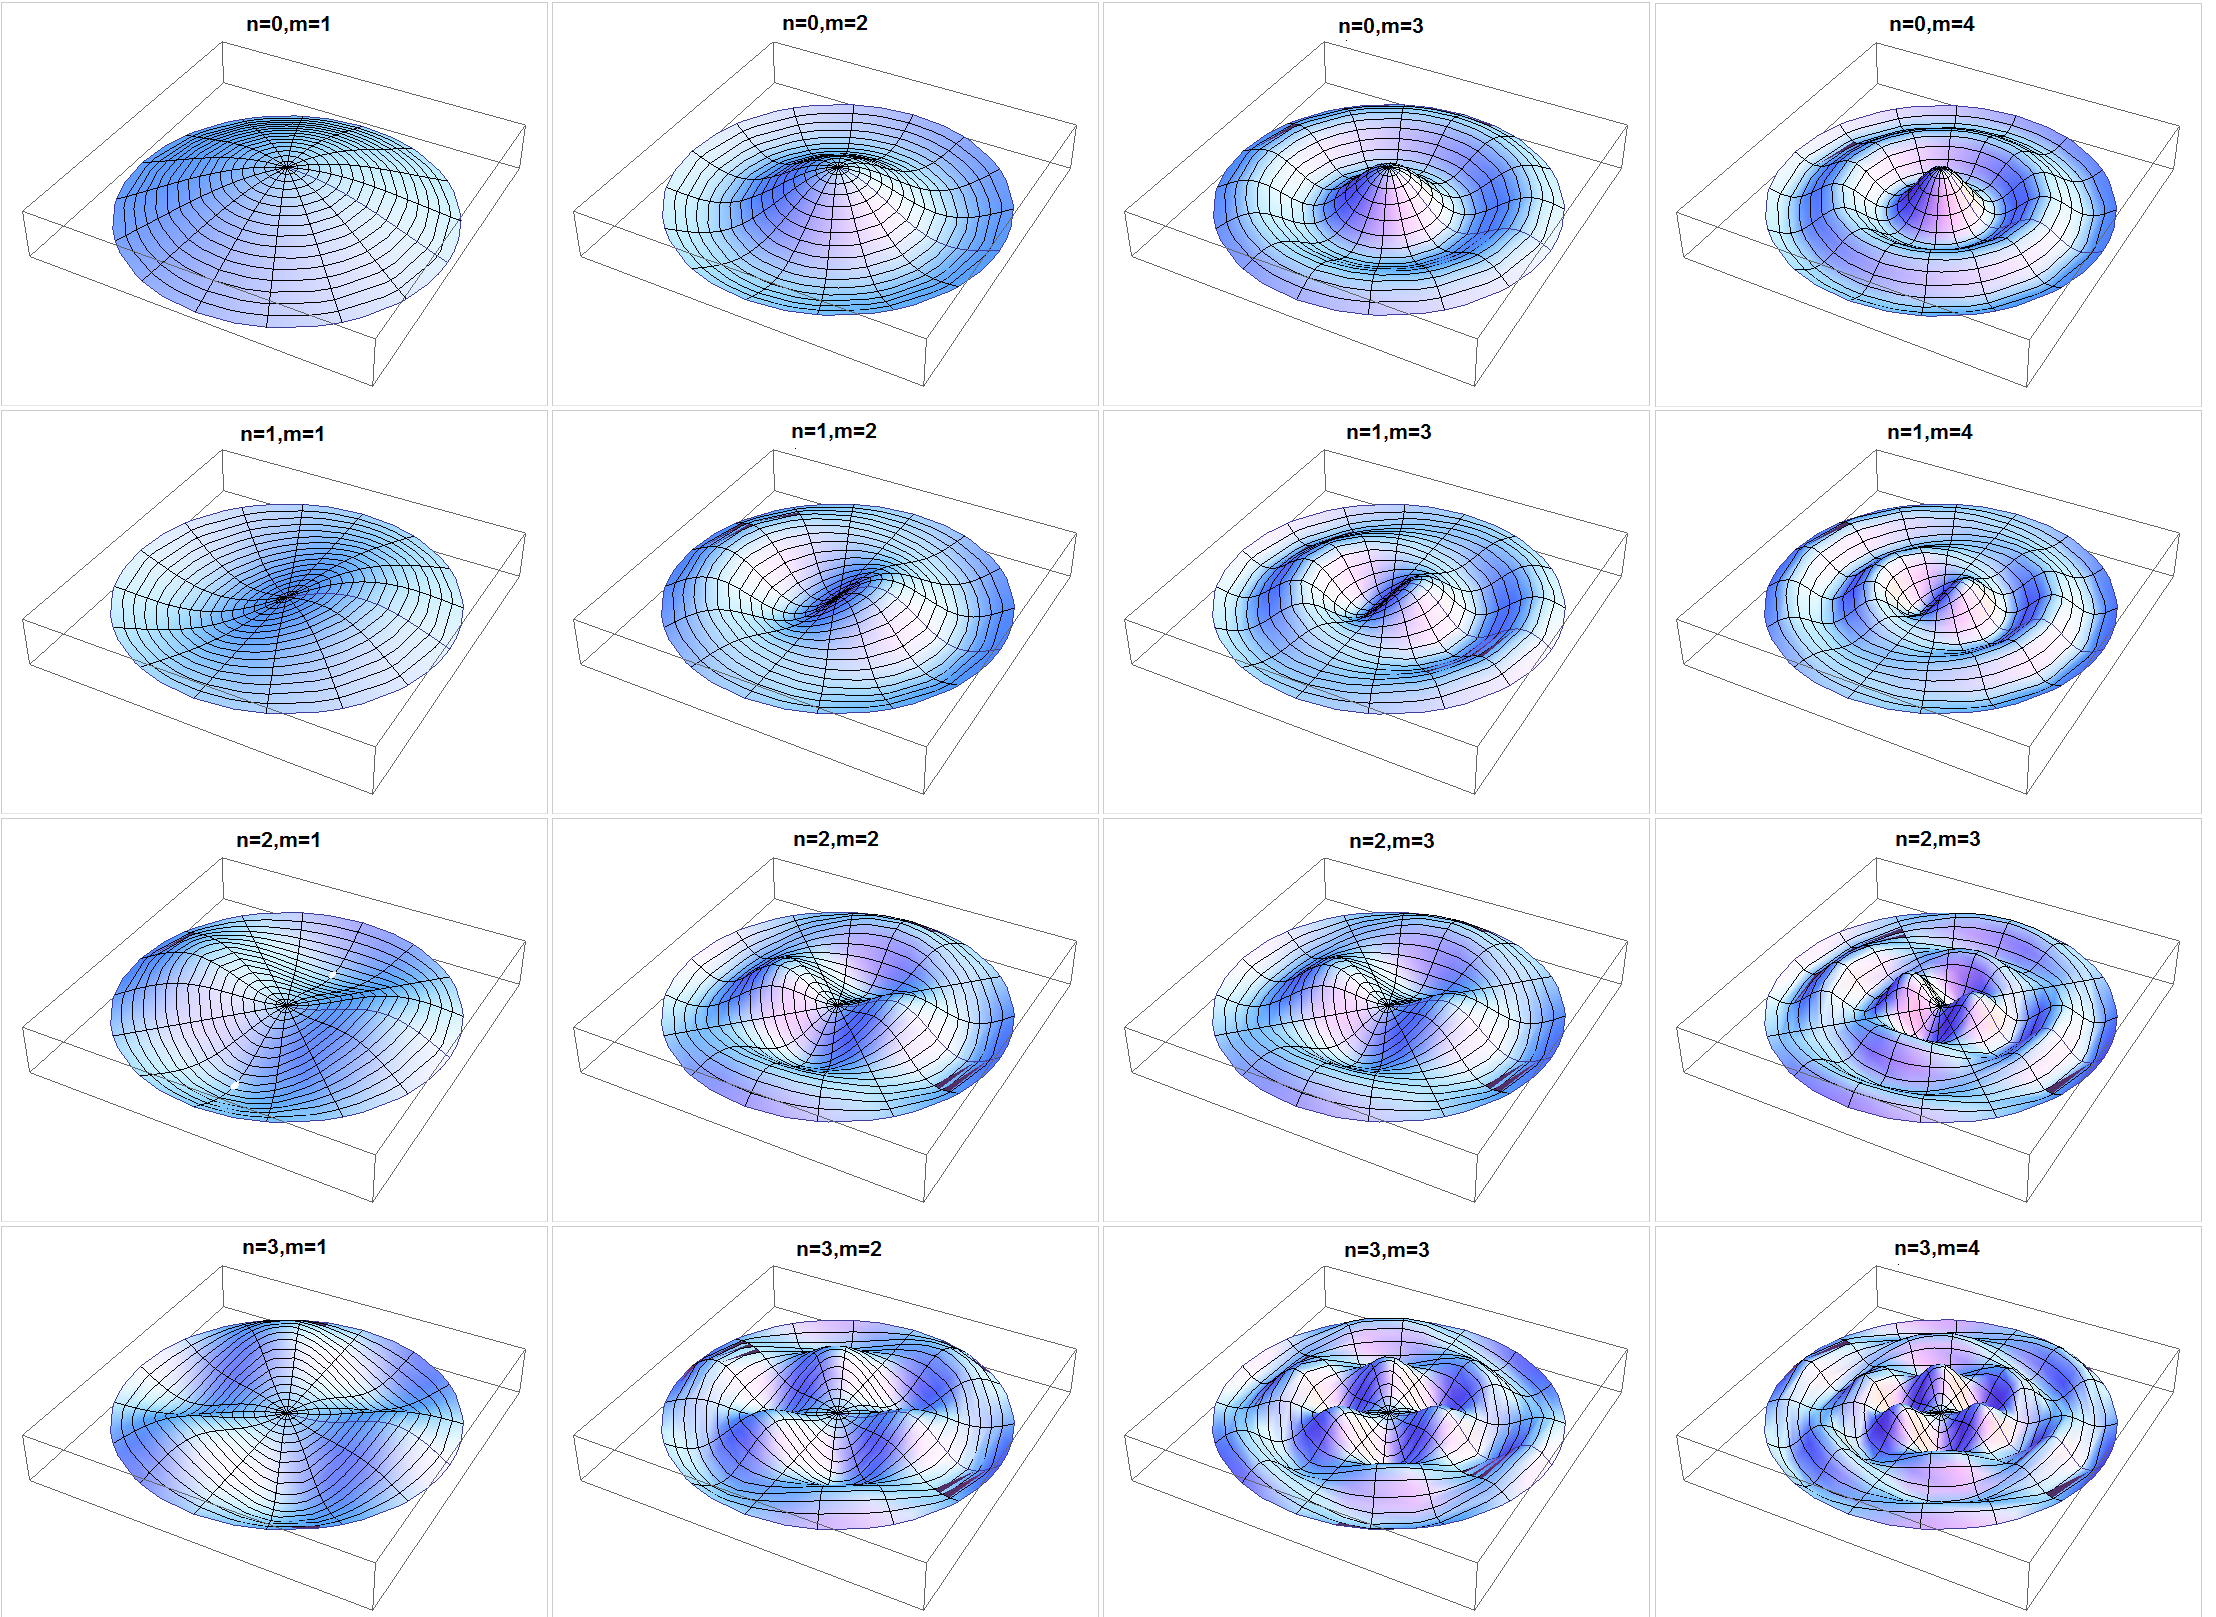
\includegraphics[width=1.1\textwidth]{DrumVibration1.png}}
		\caption{Solutions of the 2D wave equation on a disc (representing the modes of vibration of a drum). Note that this figure switches $m$ and $n$ from our usage. (source: \href{http://www.bio-physics.at/wiki/index.php?title=File:Vibrations.png}{bio-physics-wiki}).}
		\label{fig:wave2d}
	\end{figure}
\end{enumerate}

\subsubsection{More General Case}

So far, we have only considered a certain case of the wave equation - with wave speed $c=1$, the initial speed being zero everywhere, and radius 1 in the disc case. Out of interest, we now state the solutions in the general case:

\begin{enumerate}
	\item \textbf{General case on a rectangle.}
	
	We solve
	\[
	u_{tt} = c^2(u_{xx} + u_{yy}), \quad 0 \leq x \leq a, \,\, 0 \leq y \leq b
	\]
	with the following boundary and initial conditions
	\begin{equation*}
		\begin{alignedat}{2}
			u(0,y,t) &= u(a,y,t) = 0, \qquad u(x,y,0) &&= f(x,y), \\
			u(x,0,t) &= u(x,b,t) = 0, \qquad u_t(x,y,0) &&= g(x,y).
		\end{alignedat}
	\end{equation*}
	The general solution is
	\[
	u(x,y,t) = \sum_{n=1}^{\infty} \sum_{m=1}^{\infty} \left(A_{mn}\cos(\lambda_{mn}t) + A_{mn}^*\sin(\lambda_{mn}t) \right) \sin(\mu_m x) \sin(\nu_n y).
	\]
	where
	\[
	\mu_m = \frac{m\pi}{a}, \quad \nu_n = \frac{n\pi}{b}, \quad \lambda_{mn} = c\sqrt{\mu_m^2 + \nu_n^2},
	\]
	and the coefficients are given by
	\begin{align*}
		A_{mn} &= \frac{4}{ab} \int_0^a \int_0^b f(x,y) \sin(\mu_m x) \sin(\nu_n y) \,dy\,dx, \\
		A_{mn}^* &= \frac{4}{ab\lambda_{mn}} \int_0^a \int_0^b g(x,y) \sin(\mu_m x) \sin(\nu_n y) \,dy\,dx.
	\end{align*}
	
	\item \textbf{General case on a disc.}
	
	We solve
	\[
	\p_{tt}u = c^2\left(u_{rr} + \frac{1}{r}u_r + \frac{1}{r^2}u_{\theta\theta}\right), \quad 0 \leq r \leq a
	\]
	with the following boundary and conditions
	\begin{align*}
		u(r,\theta,0) &= f(r,\theta), \qquad u(a,\theta,t) = 0, \\
		u_t(r,\theta,0) &= g(r,\theta).
	\end{align*}
	The general solution is
	\begin{align*}
		u(r,\theta,t) = &\sum_{m=0}^{\infty} \sum_{n=1}^{\infty} \underbrace{\left(A_{mn}\cos(m\theta) + B_{mn}\sin(m\theta)\right) J_m(\lambda_{mn}r) \cos(c\lambda_{mn}t)}_{u_{mn}(r,\theta,t)} \\
		+ &\sum_{m=0}^{\infty} \sum_{n=1}^{\infty} \underbrace{\left(A_{mn}^*\cos(m\theta) + B_{mn}^*\sin(m\theta)\right) J_m(\lambda_{mn}r) \sin(c\lambda_{mn}t)}_{u_{mn}^*(r,\theta,t)},
	\end{align*}
	where
	\[
	\lambda_{mn} = \frac{\mu_{mn}}{a},
	\]
	and $\mu_{mn}$ is the $n$th positive zero of $J_m$. So we can see that the solution is split into two series - one relating to the initial shape, the other to the initial velocity.
	
	The coefficients related to $u_{mn}(r,\theta,t)$ are
	\begin{align}
		A_{0n} &= \frac{1}{\pi a^2J_1^2(\mu_{0n})} \int_0^{2\pi} \int_0^a f(r,\theta) J_0(\lambda_{0n}r) r \,dr\,d\theta \\
		\label{eq:wave2dgen1}
		A_{mn} &= \frac{2}{\pi a^2J_{m+1}^2(\mu_{mn})} \int_0^{2\pi} \int_0^a f(r,\theta) \cos(m\theta) J_m(\lambda_{mn}r) r \,dr\,d\theta \\
		B_{mn} &= \frac{2}{\pi a^2J_{m+1}^2(\mu_{mn})} \int_0^{2\pi} \int_0^a f(r,\theta) \sin(m\theta) J_m(\lambda_{mn}r) r \,dr\,d\theta,
	\end{align}
	and the coefficients related to $u_{mn}^*(r,\theta,t)$ are
	\begin{align}
		A_{0n}^* &= \frac{1}{\pi c\mu_{0n} aJ_1^2(\mu_{0n})} \int_0^{2\pi} \int_0^a g(r,\theta) J_m(\lambda_{0n}r) r \,dr\,d\theta \\
		A_{mn}^* &= \frac{2}{\pi c\mu_{mn} aJ_{m+1}^2(\mu_{mn})} \int_0^{2\pi} \int_0^a g(r,\theta) \cos(m\theta) J_m(\lambda_{mn}r) r \,dr\,d\theta \\
		B_{mn}^* &= \frac{2}{\pi c\mu_{mn} aJ_{m+1}^2(\mu_{mn})} \int_0^{2\pi} \int_0^a g(r,\theta) \sin(m\theta) J_m(\lambda_{mn}r) r \,dr\,d\theta,
	\end{align}
	for $m,n \in \mathbb{N}$.
\end{enumerate}

\subsubsection{Examples}

Note that while these examples follow the statement of the general case of the 2D wave equation, they are in fact (nearly) example of the specific cases we solved in \Cref{sec:waveeqn2dne}. The only difference is that in \Cref{eg:waveeqn2drect}, we take $c=6$ instead of $c=1$ for wave speed.

\begin{eg}\label{eg:waveeqn2drect}
	A $2 \times 3$ rectangular membrane, with $c=6$, is deformed to have an initial shape given by
	\[
	f(x,y) = xy(2-x)(3-y).
	\]
	The edges of this membrane are kept fixed, and it is released at $t=0$. We wish to find an expression for the shape of the membrane for $t>0$.
	
	Since the membrane starts from rest, $A_{mn}^* = 0$ immediately, Then
	\begin{align*}
		A_{mn} &= \frac{4}{ab} \int_0^a \int_0^b f(x,y) \sin(\mu_m x) \sin(\nu_n y) \,dy\,dx \\
		&= \frac23 \int_0^2 \int_0^3 xy(2-x)(3-y) \sin\left(\frac{m\pi x}{2}\right) \sin\left(\frac{n\pi y}{3}\right) \,dy\,dx \\
		&= \frac23 \int_0^2 x(2-x) \sin\left(\frac{m\pi x}{2}\right) \,dx \int_0^3 y(3-y) \sin\left(\frac{n\pi y}{3}\right) \,dy \\
		&= \frac23 \left(\frac{16\left(1+(-1)^{m+1}\right)}{\pi^3 m^3}\right) \left(\frac{54\left(1+(-1)^{n+1}\right)}{\pi^3 n^3}\right) \\
		&= \frac{576}{\pi^6} \frac{\left(1+(-1)^{m+1}\right) \left(1+(-1)^{n+1}\right)}{m^3n^3}.
	\end{align*}
	In this working, we write
	\[
	\int_0^2 x(2-x) \sin\left(\frac{m\pi x}{2}\right) \,dx = 2\int_0^2 x \sin\left(\frac{m\pi x}{2}\right) \,dx - \int_0^2 x^2 \sin\left(\frac{m\pi x}{2}\right) \,dx,
	\]
	then use the fact that
	\begin{align*}
		\int x\sin(ax)\,dx &= -\frac{x\cos(ax)}{a} + \frac{\sin(ax)}{a^2} + C \\
		\int x^2\sin(ax)\,dx &= -\frac{x^2\cos(ax)}{a} + \frac{2x\sin(ax)}{a^2} + \frac{2\cos(ax)}{a^3} + C
	\end{align*}
	to find the definite integral between 0 and 2 for $a = \frac{m\pi}{2}$. A similar method works for calculating the second integral.
	
	The coefficients $\lambda_{mn}$ are given by
	\[
	\lambda_{mn} = 6\sqrt{\frac{m^2\pi^2}{2^2} + \frac{n^2\pi^2}{3^2}} = \pi\sqrt{9m^2+4n^2}.
	\]
	Assembling these pieces yields a general solution of
	\[
	u(x,y,t) = \frac{576}{\pi^6} \sum_{n=1}^{\infty} \sum_{m=1}^{\infty} \frac{\left(1+(-1)^{m+1}\right) \left(1+(-1)^{n+1}\right)}{m^3n^3} \cos\left(\pi\sqrt{9m^2+4n^2}t\right) \sin\left(\frac{m\pi x}{2}\right) \sin\left(\frac{n\pi y}{3}\right).
	\]
\end{eg}

\begin{exercise}
	Suppose you are a masochist (why else would you attempt this?) In addition, suppose that in the previous example we also impose an initial velocity of $g(x,y) = \sin(2\pi x)$. Find the shape of the membrane for time $t>0$ in this case.
\end{exercise}

\begin{remark}
	With the 2D wave equation on a disc, if $f$ is such that $f(r,\theta)=f(r)$) (i.e. $f$ is radially symmetric), then for $m \neq 0$, $A_{mn} = 0$ and $B_{mn} = 0$ also. In other words, there are only the $A_{0n}$ terms.
	
	Likewise, if $g$ is radially symmetric, then there are only $A_{0n}^*$ terms.
\end{remark}

\begin{proof}
	Beginning with \Cref{eq:wave2dgen1},
	\begin{align*}
		A_{mn} &= \frac{2}{\pi a^2J_{m+1}^2(\mu_{mn})} \int_0^{2\pi} \int_0^a f(r,\theta) \cos(m\theta) J_m(\lambda_{mn}r) r \,dr\,d\theta,
		\intertext{and replacing $f(r,\theta)$ with $f(r)$,}
		&= (\cdots) \int_0^{2\pi} \int_0^a f(r) \cos(m\theta) J_m(\lambda_{mn}r) r \,dr\,d\theta \\
		&= (\cdots)  \int_0^a f(r) J_m(\lambda_{mn}r) r \,dr \underbrace{\int_0^{2\pi} \cos(m\theta) \,d\theta}_{=0},
	\end{align*}
	and similarly for $B_{mn}$.
\end{proof}

This remark is very useful in the following example:

\begin{eg}
	Solve the wave equation in two dimensions with $a=c=1$ and initial conditions
	\[
	f(r,\theta)=1-r^4, \quad g(r,\theta)=0.
	\]
	Because $g(r,\theta)=0$, we do not need to worry about the $A_{mn}^*$ and $B_{mn}^*$ terms. In addition, because $f$ is radially symmetric, we only need to compute $A_{0n}$:
	\begin{align*}
		A_{0n} &= \frac{1}{\pi J_1^2(\mu_{0n})} \int_0^{2\pi} \int_0^1 f(r) J_0(\mu_{0n}r) r \,dr\,d\theta \\
		&= \frac{1}{\pi J_1^2(\mu_{0n})} \int_0^{2\pi} \,d\theta \int_0^1 f(r) J_m(\mu_{0n}r) r \,dr \\
		&= \frac{2}{J_1^2(\mu_{0n})} \int_0^1 (1-r^4) J_0(\mu_{0n}r) r \,dr.
	\end{align*}
	We make the substitution $x = \mu_{0n}r$:
	\begin{align*}
		&= \frac{2}{\mu_{0n}^2 J_1^2(\mu_{0n})} \int_0^{\mu_{0n}} \left( 1-\frac{x^4}{\mu_{0n}^4} \right) J_0(x) x \,dx \\
		&= \frac{2}{\mu_{0n}^2 J_1^2(\mu_{0n})} \left( \underbrace{\int_0^{\mu_{0n}} xJ_0(x) \,dx}_{A} - \frac{1}{\mu_{0n}^4} \underbrace{\int_0^{\mu_{0n}} x^5J_0(x) \,dx}_{B}\right). 
	\end{align*}
	From here, we find\footnote{The first of these can be found by integrating the power series for $J_0(x)$ in \Cref{eq:besselfirstkind}, making use of the fact that $\Gamma(k+1)=k!$:
		\[
		xJ_0(x) = x \sum_{k=0}^{\infty} (-1)^k\frac{(\frac{x^2}{4})^k}{k!\Gamma(k+1)} = x \sum_{k=0}^{\infty} \frac{(-1)^k}{4^k(k!)^2}x^{2k+1}.
		\]
		Therefore
		\begin{align*}
			\int xJ_0(x) \,dx &= \int \sum_{k=0}^{\infty} \frac{(-1)^k}{4^k(k!)^2}x^{2k+1} \,dx = \sum_{k=0}^{\infty} \frac{(-1)^k}{4^k(k!)^2(2k+2)}x^{2k+2} \\
			&= \frac{x^2}{2} \sum_{k=0}^{\infty} \frac{(-1)^k}{4^kk!(k+1)!}x^{2k} = x \cdot \frac{x}{2} \sum_{k=0}^{\infty} (-1)^k\frac{(\frac{x^2}{4})^k}{k!\Gamma(k+2)} = xJ_1(x).
		\end{align*}
		Alternatively, we know from \cite[Eq. 9.1.30]{olver} that
		\[
		\frac{d}{dx}\left(x^pJ_p(x)\right) = x^pJ_{p-1}(x),
		\]
		and setting $p=1$ and integrating both sides gives the desired result.}
	\begin{align*}
		A = \int_0^{\mu_{0n}} xJ_0(x) \,dx &= \left[xJ_1(x)\right]_0^{\mu_{0n}} = \mu_{0n}J_1(\mu_{0n}) \\
		B = \int_0^{\mu_{0n}} x^5J_0(x) \,dx &= \left[x^5J_1(x) - 4x^4J_2(x) + 8x^3J_3(x)\right]_0^{\mu_{0n}} \\
		&= \mu_{0n}^5J_1(\mu_{0n}) - 4\mu_{0n}^4J_2(\mu_{0n}) + 8\mu_{0n}^3J_3(\mu_{0n}).
	\end{align*}
	It follows that
	\[
	A_{0n} = \frac{2}{\mu_{0n}^2 J_1^2(\mu_{0n})} \left(A - \frac{1}{\mu_{0n}^4}B\right) = \frac{8\left(\mu_{0n}J_2(\mu_{0n}) - 2J_3(\mu_{0n})\right)}{\mu_{0n}^3J_1^2(\mu_{0n})},
	\]
	so that finally
	\[
	u(r,\theta,t) = \sum_{n=1}^{\infty} \frac{8\left(\mu_{0n}J_2(\mu_{0n}) - 2J_3(\mu_{0n})\right)}{\mu_{0n}^3J_1^2(\mu_{0n})} J_0(\mu_{0n}r)\cos(\mu_{0n}t).
	\]
\end{eg}
\section{The Laplace Transform}

While the methods used to solve second-order linear ODEs that were introduced in SVCDE and seen again in this course are useful, they can be awkward and time-consuming to apply in practice. The method involving the Laplace transform is useful more generally, and in particular in the cases where the ODE has impulsive forcing or discontinuous forcing. We shall introduce it now.

\subsection{Introduction}

\begin{definition}
	The Laplace transform $F(s)$ of $f(t)$ is
	\begin{equation}
		F(s) = \Lap{f}(s) = \int_0^{\infty} e^{-st}f(t)\,dt = \lim_{T \to \infty} \int_0^T e^{-st}f(t)\,dt.
	\end{equation}
\end{definition}

\begin{eg}\label{eg:laplacetrans}\hfill
	\begin{itemize}
		\item For $f(t)=1$,
		\[
			F(s) = \int_0^{\infty} e^{-st}\,dt = \left[\frac{e^{-st}}{-s}\right]_0^{\infty} = \frac{1}{s}. \tag{$s>0$}
		\]
		\item For $f(t)=e^{at}$,
		\[
			F(s) = \int_0^{\infty} e^{-st}e^{at}\,dt = \left[\frac{e^{-(s-a)t}}{-(s-a)}\right]_0^{\infty} = \frac{1}{s-a}. \tag{$s>a$}
		\]
		\item For $f(t) = \sin(at)$,
		\begin{align*}
			F(s) &= \int_0^{\infty} e^{-st}\sin(at) \,dt \\
			&= \left[e^{-st}\frac{\cos(at)}{a}\right]_0^{\infty} - \frac{s}{a}\int_0^{\infty} e^{-st}\cos(at) \,dt \\
			&= \frac{1}{a} - \frac{s}{a}\int_0^{\infty} e^{-st}\cos(at) \,dt \\
			&= \frac{1}{a} - \frac{s^2}{a^2}\int_0^{\infty} e^{-st}\sin(at) \,dt \\
			\left(1+\frac{s^2}{a^2}\right) F(s) &= \frac{1}{a} \\
			F(s) &= \frac{a}{s^2+a^2}. \tag{$s>0$}
		\end{align*}
		\item For $f(t) = \cos(at)$,
		\[
			F(s) = \frac{s}{s^2+a^2}.
		\]
		
	\end{itemize}
\end{eg}

Another way of writing the above results is that $\Lap{e^{at}} = \frac{1}{s-a}$, etc.

\begin{theorem}
	The Laplace transform of $f(t)$ exists for $s$ large enough provided that
	\begin{itemize}
		\item $f(t)$ is piecewise continuous,
		\item $|f(t)| \leq Ae^{Bt}$.
	\end{itemize}
\end{theorem}

In this theorem, the first condition is necessary for the integral $\int_0^{\infty} e^{-st}f(t)\,dt$ to exist. The second condition is necessary to bound $F(s)$:
\[
|F(s)| \leq \int_0^{\infty} e^{-st}|f(t)|\,dt \leq A\int_0^{\infty} e^{-st}e^{Bt}\,dt < \infty \quad\text{if } s>B.
\]

Key Properties of the Laplace transform:
\begin{enumerate}
	\item Linearity: $\Lap{c_1f_1(t) + c_2f_2(t)} = c_1\Lap{f_1} + c_2\Lap{f_2}$.
	\item $\Lap{f'} = s\Lap{f} - f(0)$.
\end{enumerate}

\begin{proof}\hfill
	\begin{enumerate}
		\item Follows easily from the linearity of the integral.
		\item Assuming the Laplace transform $\Lap{f}$ is well-defined,
		\begin{align*}
			\Lap{f'} = \int_0^{\infty} e^{-st}f'(t)\,dt &= \left[e^{-st}f(t)\right]_0^{\infty} + s\int_0^{\infty} e^{-st}f(t)\,dt \\
			&= s\Lap{f} - f(0).
		\end{align*}
	\end{enumerate}
\end{proof}

The Laplace transform for higher derivatives may be computed using the equation for $\Lap{f'}$:
\begin{align*}
	\Lap{f^{(n)}} &= s\Lap{f^{(n-1)}} - f^{(n-1)}(0) \\
	&= s^2\Lap{f^{(n-2)}} - sf^{(n-2)}(0) - f^{(n-1)}(0) \\
	&= s^n\Lap{f} - s^{n-1}f(0) - s^{n-2}f'(0) - \cdots - f^{(n-1)}(0).
\end{align*}

\subsection{Solving ODEs}

The method of using the Laplace transform to solve second-order linear ODEs is best illustrated with an example.

\begin{eg}
	We solve the ODE
	\[
	y''-y'-2y = 0 \quad\text{with}\quad y(0)=1, \,\,y'(0)=0.
	\]
	We apply the Laplace transform to the whole equation, writing $Y(s) = \Lap{y}$ and using the initial conditions to simplify:
	\begin{align*}
		s^2Y(s) - s\cancelto{1}{y(0)} - \cancelto{0}{y'(0)} - sY(s) + \cancelto{1}{y(0)} - 2Y(s) &= 0 \\
		(s^2-s-2)Y(s) &= s-1 \\
		Y(s) &= \frac{s-1}{s^2-s-2}.
	\end{align*}
	Now that we know $Y(s)$, what we really want is a formula to invert the Laplace transform and recover $y(t)$. In fact, such a formula exists:
	\[
	y(t) = \frac{1}{2\pi i} \int_{\gamma-i\infty}^{\gamma+i\infty} e^{st}Y(s) \,ds.
	\]
	However, this formula is quite complicated to apply, as it involves integrating along the line $\Re(s) = \gamma$ in the complex plane. Therefore, we shall generally invert the Laplace transform by inspection.
	
	Recall from \Cref{eg:laplacetrans} that $\Lap{e^{at}} = \frac{1}{s-a}$. We can write $Y(s)$ in this form by using partial fractions:
	\begin{align*}
		Y(s) = \frac{s-1}{s^2-s-2} &= \frac{A}{s-2} + \frac{B}{s+1} \\
		&= \frac13\cdot\frac{1}{s-2} + \frac23\cdot\frac{1}{s+1} \\
		&= \frac13\Lap{e^{2t}} + \frac23\Lap{e^{-t}} \\
		\implies y(t) &= \frac13e^{2t} + \frac23e^{-t}.
	\end{align*}
	This can easily be checked by applying the methods we know from before of finding the characteristic equation, getting exponential solutions, applying the initial conditions, and so on.
\end{eg}

\begin{eg}
	We solve the ODE
	\[
	y''+y = \sin(2t) \quad\text{with}\quad y(0)=2, \,\,y'(0)=1.
	\]
	Applying the Laplace transform and using the initial conditions:
	\begin{align*}
		s^2Y - 2s - 1 + Y &= \frac{2}{s^2+4} \\
		(s^2+1)Y &= \frac{2}{s^2+4} +2s+1 \\
		(s^2+1)Y &= \frac{2s^3+s^2+8s+6}{s^2+4} \\
		Y(s) &= \frac{2s^3+s^2+8s+6}{(s^2+1)(s^2+4)}.
	\end{align*}
	We wish to write $Y(s)$ as its partial fraction decomposition:
	\begin{align*}
		Y(s) = \frac{2s^3+s^2+8s+6}{(s^2+1)(s^2+4)} &= \frac{As+B}{s^2+1} + \frac{Cs+D}{s^2+4} \\
		2s^3+s^2+8s+6 &= (As+B)(s^2+4) + (Cs+D)(s^2+1).
	\end{align*}
	Equating coefficients gives the following system of equations:
	\begin{equation*}
		\begin{alignedat}{2}
			&s^3 &&: 2 = A+C \\
			&s^2 &&: 1 = B+D \\
			&s &&: 8 = 4A+C \\
			&s^0 &&: 6 = 4B+D.
		\end{alignedat}
	\end{equation*}
	Subtracting the first equation from the third yields
	\[
	3A = 6 \implies A = 2 \implies C=0,
	\]
	and subtracting the second equation from the fourth gives
	\[
	3B = 5 \implies B = \frac53 \implies D = -\frac23.
	\]
	Therefore
	\begin{align*}
		Y(s) &= \frac{2s}{s^2+1} + \frac53\cdot\frac{1}{s^2+1} - \frac13\cdot\frac{2}{s^2+4} \\
		&= 2\Lap{\cos{t}} + \frac53\Lap{\sin{t}} - \frac13\Lap{\sin(2t)} \\
		\implies y(t) &= 2\cos{t} + \frac53\sin{t} - \frac13\sin(2t).
	\end{align*}
\end{eg}

\subsection{Calculating the Laplace Transform for More Functions}

Now that we've seen how to use the Laplace transform to solve ODE, we see that it's important to have a `dictionary' of functions $f(t)$ and their transform $F(s)$. In that vein, we build on the few transforms found in \Cref{eg:laplacetrans}.

More properties of the Laplace transform:
\begin{enumerate}
	\item s-shift: $\Lap{e^{-ct}f(t)} = F(s+c)$.
	\item t-shift: $\Lap{f(t-c)} = e^{-sc}F(s)$ if $c \geq 0$ and $f(t)=0$ for $t<0$.
	\item Derivative in $s$: $\Lap{tf(t)} = -\frac{d}{ds}F(s)$.
	\item Scaling: $\Lap{f(ct)} = \frac{1}{c} F\left(\frac{s}{c}\right)$.
\end{enumerate}

\begin{proof}\hfill
	All three properties essentially follow from the definition of the Laplace transform.
	\begin{enumerate}
		\item \[\Lap{e^{-ct}f(t)} = \int_0^{\infty} e^{-st}e^{-ct}f(t) \,dt = \int_0^{\infty} e^{-(s+c)t}f(t) \,dt = F(s+c).\]
		\item Let $u=t-c$, then
		\[
			\int_0^{\infty} e^{-st}f(t-c) \,dt = \int_{-c}^{\infty} e^{-s(u+c)}f(u) \,du = \int_0^{\infty} e^{-sc}e^{-su}f(u) \,du = e^{-sc}F(s).
		\]
		\item \[\Lap{tf(t)} = \int_0^{\infty} e^{-st}tf(t) \,dt = \int_0^{\infty} -\frac{d}{ds}\left(e^{-st}\right) f(t) \,dt = -\frac{d}{ds} \int_0^{\infty} e^{-st}f(t) \,dt = -\frac{d}{ds}F(s).\]
		\item We have
		\[
		\Lap{f(ct)} = \int_0^{\infty} e^{-st}f(ct)\,dt = \int_0^{\infty} e^{-(s/c)ct}f(ct)\,dt.
		\]
		Making a change of variables $u=ct$ (with $dt = \frac{1}{c}du$) yields
		\[
		\Lap{f(ct)} = \int_0^{\infty} e^{-(s/c)ct}f(ct)\,dt = \frac{1}{c} \int_0^{\infty} e^{-(s/c)u}f(u)\,du = \frac{1}{c} F\left(\frac{s}{c}\right).
		\]
	\end{enumerate}
\end{proof}

\begin{eg}
	Using these properties, we calculate the Laplace transform for a few more functions.
	\begin{itemize}
		\item First, using the s-derivative property,
		\[
		\Lap{t} = \Lap{t\cdot 1} = -\frac{d}{ds}\Lap{1} = -\frac{d}{ds} \frac{1}{s} = \frac{1}{s^2}.
		\]
		\item By repeated application of the s-derivative,
		\[
		\Lap{t^n} = \frac{n!}{s^{n+1}}.
		\]
		\item Also using the s-derivative,
		\[
		\Lap{te^{at}} = -\frac{d}{ds} \Lap{e^{at}} = -\frac{d}{ds} \frac{1}{s-a} = \frac{1}{(s-a)^2}.
		\]
		\item Applying the s-shift property to $\Lap{\cos(at)} = \frac{s}{s^2+a^2}$,
		\[
		\Lap{e^{bt}\cos(at)} = \frac{s-b}{(s-b)^2+a^2}.
		\]
		\item Similarly, applying the s-shift to $\Lap{\sin(at)} = \frac{a}{s^2+a^2}$ gives,
		\[
		\Lap{e^{bt}\sin(at)} = \frac{a}{(s-b)^2+a^2}.
		\]
		\item By repeated application of the s-derivative, we can find that
		\[
		\Lap{t^nf(t)} = (-1)^n \frac{d}{ds}F(s).
		\]
		\item Using the previous result, we find
		\[
		\Lap{t^ne^{bt}\cos(at)} = (-1)^n\frac{d}{ds} \left(\frac{s-b}{(s-b)^2+a^2}\right),
		\]
		and a similar relation for $\Lap{t^ne^{bt}\sin(at)}$:
		\[
		\Lap{t^ne^{bt}\sin(at)} = (-1)^n\frac{d}{ds} \left(\frac{a}{(s-b)^2+a^2}\right).
		\]
	\end{itemize}
\end{eg}

Overall, what this example tells us is that when we apply the Laplace transform to functions of the form $g(t) = t^ne^{bt}\cos(at)$ and $h(t) = t^ne^{bt}\sin(at)$ (i.e. those that are a product of a power, exponential, and trigonometric function) the result is a rational function. These functions $g$ and $h$ are precisely the types of functions that appear as the RHS in ODEs we have solved previously using, for example, the method of undetermined coefficients. Thus, it is very helpful that we can get back to them by inverting the Laplace transform from a rational function.

\begin{remark}
	It is also possible to find $\Lap{e^{at}}$ using the s-shift property applied to $\Lap{1} = \frac{1}{s}$.
\end{remark}

For reference, a table of elementary Laplace transforms is given in \Cref{table:laplace} in \Cref{sec:laptable}.

\begin{eg}
	We solve the ODE
	\[
	y''-2y'+2y=2e^t \quad\text{with}\quad y(0)=0, \,\,y'(0)=1.
	\]
	Applying the Laplace transform:
	\begin{align*}
		s^2Y(s) - s\cancelto{0}{y(0)} - \cancelto{1}{y'(0)} - 2sY(s) + 2\cancelto{0}{y(0)} + 2Y(s) &= \frac{2}{s-1} \\
		s^2Y(s) - 1 - 2sY(s) + 2Y(s) &= \frac{2}{s-1} \\
		(s^2-2s+2)Y(s) &= \frac{2}{s-1} + 1 \\
		(s^2-2s+2)Y(s) &= \frac{s+1}{s-1} \\
		Y(s) &= \frac{s+1}{(s-1)(s^2-2s+2)}.
	\end{align*}
	As before, we write $Y(s)$ in terms of partial fractions:
	\begin{align*}
		Y(s) = \frac{s+1}{(s-1)(s^2-2s+2)} &= \frac{A}{s-1} + \frac{Bs+C}{(s-1)^2+1} \\
		s+1 &= A((s-1)^2+1) + (Bs+C)(s-1).
	\end{align*}
	Choosing $s=1$ tells us that $A=2$. For finding $B$ and $C$, we equate coefficients:
	\begin{align*}
		&s^2 : 0 = A+B \implies B=-2 \\
		&s^0 : 1 = 2A-C \implies C=3.
	\end{align*}
	Hence
	\begin{align*}
		Y(s) &= \frac{2}{s-1} - \frac{2s-3}{(s-1)^2+1} \\
		&= \frac{2}{s-1} - \frac{2(s-1)-1}{(s-1)^2+1} \\
		&= \frac{2}{s-1} - 2\frac{s-1}{(s-1)^2+1} + \frac{1}{(s-1)^2+1} \\
		&= 2\Lap{e^t} - 2\Lap{e^t\cos{t}} + \Lap{e^t\sin{t}} \\
		\implies y(t) &= 2e^t - 2e^t\cos{t} + e^t\sin{t}.
	\end{align*}
\end{eg}

\subsection{Solving ODEs with Discontinuous Forcing}

The Laplace transform is particularly efficient in solving ODEs where the RHS is a discontinuous function.

To work with such ODEs, we first introduce the \vb{unit step function} (also known as the Heaviside function):
\begin{equation}
	u_c(t) = \begin{cases}0 & \text{if } t<c \\ 1 & \text{if } t \geq c\end{cases}.
\end{equation}
This function is useful when we want to `clip' a function $f(t)$, i.e. only take the part of the function between $a$ and $b$:
\[
f_{\text{clip}}(t) = f(t)\left(u_a(t) - u_b(t)\right),
\]
or shift the function so that it is zero for all $t \leq c$:
\[
f_{\text{shift}} = f(t-c)u_c(t).
\]

\begin{figure}[!ht]
	\centering
	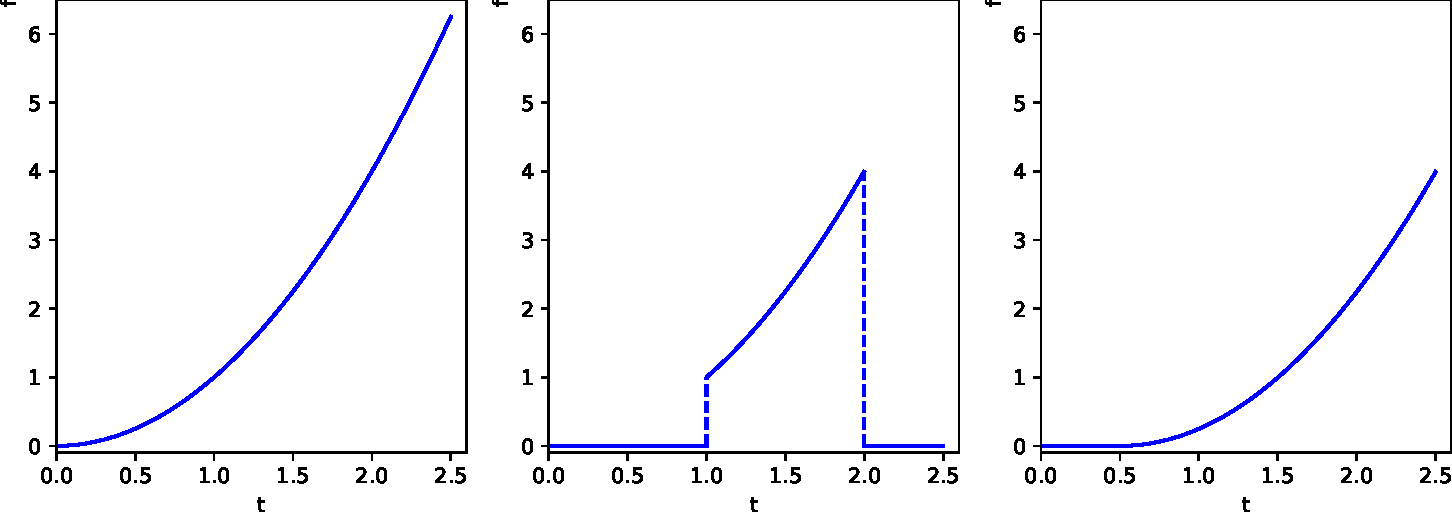
\includegraphics[width=0.9\textwidth]{ClippedFunctions.pdf}
	\caption{The function $f(x)=x^2$ (left), the `clipped' function with $a=1$ and $b=2$ (centre), and the `shifted' function with $c=\frac12$ (right).}
	\label{fig:clipping}
\end{figure}

The Laplace transform of the unit step function ($c \geq 0$) is
\[
	\Lap{u_c(t)} = \int_0^{\infty} e^{-st}u_c(t)\,dt = \int_c^{\infty}e^{-st}\,dt = \frac{e^{-sc}}{s}, \quad s>0.
\]
Here we can see a connection to the t-shift property of the Laplace transform from earlier, which stated that $\Lap{f(t-c)} = e^{-sc}F(s)$ if $c \geq 0$ and $f(t)=0$ for $t<0$. Functions satisfying these conditions can be nicely described as $f(t-c)u_c(t)$, thus
\begin{equation}\label{eq:laplacediscont}
	\Lap{f(t-c)u_c(t)} = e^{-sc}F(s).
\end{equation}

This property can also be proved more directly:
\begin{proof}
	From the definition of the Laplace transform,
	\[
	\Lap{f(t-c)u_c(t)} = \int_0^{\infty} e^{-st}f(t-c)u_c(t) \,dt.
	\]
	Applying the change of variables $t-c=t'$,
	\begin{align*}
		\int_0^{\infty} e^{-st}f(t-c)u_c(t) \,dt &= \int_{-c}^{\infty} e^{-s(t'+c)}f(t') \underbrace{u_c(t'+c)}_{=u_0(t')} \,dt' \\
		&= e^{-sc} \int_0^{\infty} e^{-st'}f(t') \,dt' \\
		&= e^{-sc} F(s).
	\end{align*}
\end{proof}

\begin{eg}
	Find the inverse Laplace transform of 
	\[
	F(s) = \frac{1-e^{-2s}}{s^2}.
	\]
	We will make use of the above property, and the fact that $\Lapinv{\frac{1}{s^2}} = t$.
	\begin{align*}
		f(t) &= \Lapinvb{\frac{1}{s^2}} - \Lapinvb{\frac{e^{-2s}}{s^2}} \\
		&= t - (t-2)u_2(t).
	\end{align*}
\end{eg}

Now we solve an ODE with discontinuous RHS:

\begin{eg}\label{eg:disconteg}
	We solve the ODE
	\[
	y''-2y'+2y=f(t) \quad\text{with}\quad y(0)=y'(0)=0,
	\]
	where $f(t)$ is shown in \Cref{fig:disconteg}. 
	
	\begin{figure}[!ht]
		\centering
		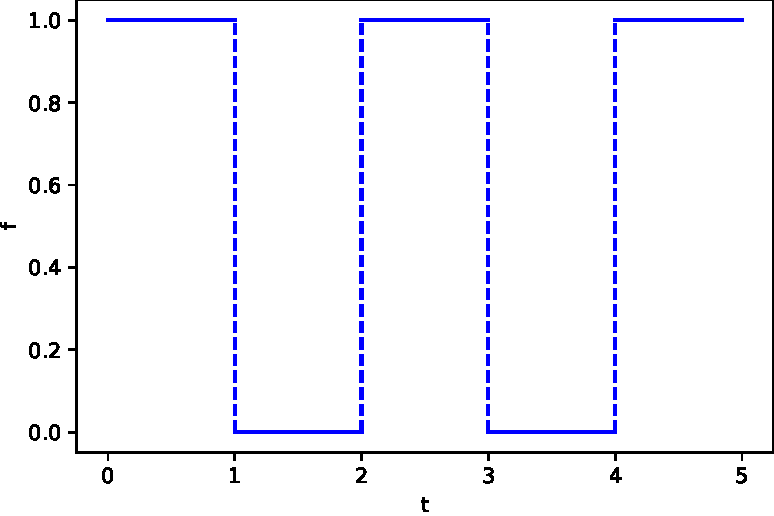
\includegraphics[width=0.6\textwidth]{DiscontEg.pdf}
		\caption{The discontinuous function $f(t)$ from \Cref{eg:disconteg}.}
		\label{fig:disconteg}
	\end{figure}
	
	We can write $f(t)$ in terms of step functions:
	\[
	f(t) = u_0(t) - u_1(t) + u_2(t) - u_3(t) + u_4(t) - u_5(t).
	\]
	Applying the Laplace transform to $f(t)$ yields
	\[
	F(s) = \frac{1-e^{-s}+e^{-2s}-e^{-3s}+e^{-4s}-e^{-5s}}{s}.
	\]
	Now we apply the Laplace transform to the entire ODE:
	\begin{align*}
		s^2Y(s) - 3sY(s) + 2Y(s) &= F(s) \\
		Y(s) = \frac{F(s)}{s^2-3s+2} &= \frac{1-e^{-s}+e^{-2s}-e^{-3s}+e^{-4s}-e^{-5s}}{s(s-1)(s-2)} \\
		&= G(s)(1-e^{-s}+e^{-2s}-e^{-3s}+e^{-4s}-e^{-5s}),
	\end{align*}
	where
	\[
	G(s) = \frac{1}{s(s-1)(s-2)} = \frac{A}{s} + \frac{B}{s-1} + \frac{C}{s-2} = \frac12\frac{1}{s} - \frac{1}{s-1} + \frac12\frac{1}{(s-2)}.
	\]
	Applying the inverse Laplace transform to $G(s)$ gives
	\[
	g(t) = \frac12\left(1 - 2e^t + e^{2t}\right),
	\]
	so by applying the property in \Cref{eq:laplacediscont}, we find the solution to be
	\[
	y(t) = g(t) - g(t-1)u_1(t) + g(t-2)u_2(t) - \cdots - g(t-5)u_5(t).
	\]
\end{eg}

\begin{eg}
	Solve the initial value problem
	\begin{align*}
		2y'' + y' + 2y &= u_5(t) - u_{20}(t) = \begin{cases}
			1, & 5 \leq t < 20 \\
			0, & 0 \leq t < 5 \text{ and } t \geq 20
		\end{cases} \\
		y(0) &+ y'(0) = 0.
	\end{align*}
	First, take the Laplace transform:
	\begin{align*}
		2s^2Y - 2sy(0) - 2y'(0) + sY - y(0) + 2Y &= \frac{e^{-5s} - e^{-20s}}{s} \\
		Y(s) &= \frac{e^{-5s} - e^{-20s}}{s(2s^2 + s + 2)} \\
		&= (e^{-5s} - e^{-20s})G(s),
	\end{align*}
	where
	\[
		G(s) = \frac{1}{s(2s^2 + s + 2)}.
	\]
	Recall the t-shift: $e^{-sc}G(s) = \Lap{g(t-c)u_c(t)}(s)$. Therefore
	\[
		y(t) = u_5(t)g(t-5) - u_{20}(t)g(t-20), \quad\text{with}\quad g(t) = \Lapinv{G(s)}.
	\]
	Now we decompose $G(s)$ into partial fractions:
	\[
		G(s) = \frac{a}{s} + \frac{bs+c}{2s^2+s+2} = \frac{1/2}{s} - \frac{s+1/2}{2s^2+s+2}.
	\]
	To deal with the second term, complete the square in the denominator:
	\[
		\frac{s+\sfrac12}{2s^2+s+2} = \frac12 \frac{(s+\sfrac14)+\sfrac14}{(s+\sfrac14)^2+\sfrac{15}{16}}.
	\]
	Using the results (see \Cref{table:laplace})
	\[
		\Lap{e^{at}\sin(bt)} = \frac{b}{(s-a)^2+b^2}, \quad \Lap{e^{at}\cos(bt)} = \frac{s-a}{(s-a)^2+b^2}
	\]
	we derive
	\[
		g(t) = \frac12 - \frac12 \left(e^{-t/4}\cos\left(\frac{\sqrt{15}}{4}t\right) + \frac{1}{\sqrt{15}} e^{-t/4}\sin\left(\frac{\sqrt{15}}{4}t\right)\right).
	\]
	Therefore the solution for $y(t)$ is
	\[
		y(t) = u_5(t)g(t-5) - u_{20}g(t-20)
	\]
	where $g(t)$ is given above.
\end{eg}

\subsection{Solving ODEs with Impulsive Forcing}

Impulsive forcing in an ODE $ay''+by'+cy=g(t)$ means that the inhomogeneity $g(t)$ acts only for a short period of time, $t_0\tau < t < t_0+\tau$.

With such an ODE, we want to impose the condition on the impulse
\[
	I(\tau) = \int_{t_0-\tau}^{t_0+\tau} g(t) \,dt = 1.
\]
This impulse provides a measure of the strength of the forcing term $g(t)$. The intuitive idea is that we are considering a forcing that is very short in duration, but large enough in magnitude that it has a significant effect on $y(t)$, for example a hammer blow in a mechanical system.

Taking $t_0$ for convenience, there are a few different options for modelling the impulse $g(t)$. They are listed below, and shown in \Cref{fig:impulsivefuncs}.
\begin{itemize}
	\item Top hat function: $g(t) = \begin{cases}\frac{1}{2\tau} & \text{if }-\tau \leq t \leq \tau \\ 0 & \text{otherwise}\end{cases}$.
	\item $g(t) = \dfrac{\tau}{\pi(t^2+\tau^2)}$
	\item Gaussian: $g(t) = \dfrac{1}{\sqrt{2\pi\tau^2}}e^{-t^2/2\tau^2}$.
\end{itemize}

\begin{figure}[!ht]
	\centering
	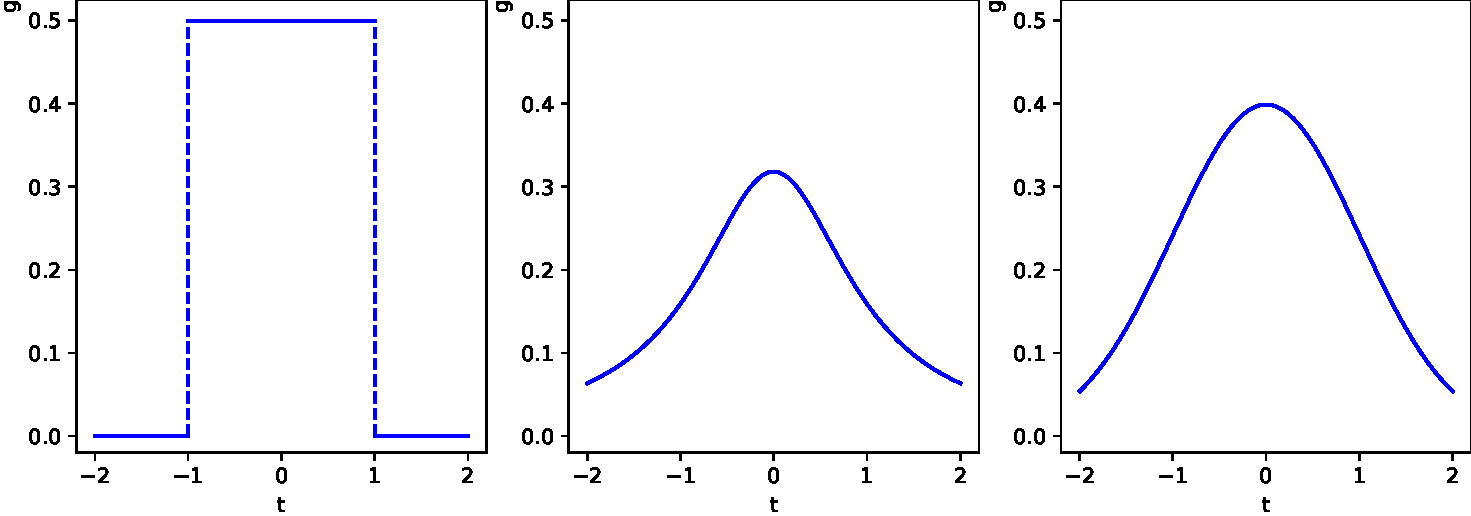
\includegraphics[width=0.9\textwidth]{ImpulsiveFunctions.pdf}
	\caption{The three examples of functions $g(t)$ for modelling impulses, setting $\tau=1$, in the order in the list from left to right.}
	\label{fig:impulsivefuncs}
\end{figure}

As $\tau \to 0$, these functions all converge to the same function: the \textbf{Dirac distribution}.

\begin{definition}
	The Dirac distribution is a ``function'' $\delta(t)$ such that
	\begin{itemize}
		\item $\delta(t)=0$ for all $t \neq 0$,
		\item $\int_{-\infty}^{\infty} \delta(t)\,dt = 1$.
	\end{itemize}
\end{definition}

With the shifted version of the Dirac distribution, it is centred at $t-t_0$ and we have $\delta(t-t_0)=0, \,\, \forall t\neq t_0$, and $\int_{-\infty}^{\infty} \delta(t-t_0)\,dt = 1$.

A key property of the Dirac distribution is that
\[
\int_{-\infty}^{\infty} f(t)\delta(t-t_0)\,dt = f(t_0).
\]
Applying the Laplace transform to the Dirac distribution:
\begin{equation*}
	\Lap{\delta(t-t_0)} = \int_0^{\infty} e^{-st}\delta(t-t_0) \,dt = e^{-st_0}. \tag{$t_0>0$}
\end{equation*}
By convention, we say that
\[
\delta(t) = \lim_{t_0 \to 0^+}\delta(t-t_0) \implies \Lap{\delta(t)} = 1.
\]

\begin{remark}
	From \Cref{eq:laplacediscont} and setting $f(t)=1$,
	\[
	\Lap{u_{t_0}(t)} = \frac{e^{-st_0}}{s}.
	\]
	Therefore
	\[
	\Lap{\delta(t-t_0)} = e^{-st_0} = s\Lap{u_{t_0}(t)} = \Lapb{\frac{d}{dt}u_{t_0}(t)}.
	\]
	Which implies that
	\[
	\text{$\delta(t-t_0)$ ``='' $\frac{d}{dt}u_{t_0}(t).$}
	\]
\end{remark}

We can do a check that $\Lap{\delta(t-t_0)} = e^{-st_0}$ makes sense by considering $\delta(t-t_0)$ as the limit as $\tau\to0$ of the top hat function in \Cref{fig:impulsivefuncs}:
\begin{align*}
	\delta(t-t_0) &= \lim_{\tau\to0} (\text{top hat function}) \\
	&= \lim_{\tau\to0} \frac{1}{2\tau}\left(u_{t_0-\tau}(t) - u_{t_0+\tau}(t)\right) = \lim_{\tau\to0} g(t,t_0).
\end{align*}
Then calculating $\Lap{g(t,t_0)}$:
\begin{align*}
	\Lap{g(t,t_0)} &= \frac{1}{2\tau} \left(\frac{e^{-s(t_0-\tau)}}{s} - \frac{e^{-s(t_0+\tau)}}{s}\right) \\
	&= \frac{e^{-st_0}}{2\tau s} (e^{s\tau}-e^{-s\tau}) \\
	&= e^{-st_0} \frac{\sinh(s\tau)}{s\tau}.
\end{align*}
Since $\lim_{x\to0} \frac{\sinh(x)}{x} = 1$, we have that
\[
\lim_{\tau\to0} \Lap{g} = e^{-st_0} = \Lap{\delta(t-t_0)}.
\]

As another check, consider the following initial value problem:
\[
y''+y = f_a(t) = \frac{1}{a}\left(u_0(t)-u_a(t)\right), \quad\text{with}\quad y(0)=y'(0)=0,
\]
where $f_a(t)$ is shown in \Cref{fig:impulseeg}.

\begin{figure}[H]
	\centering
	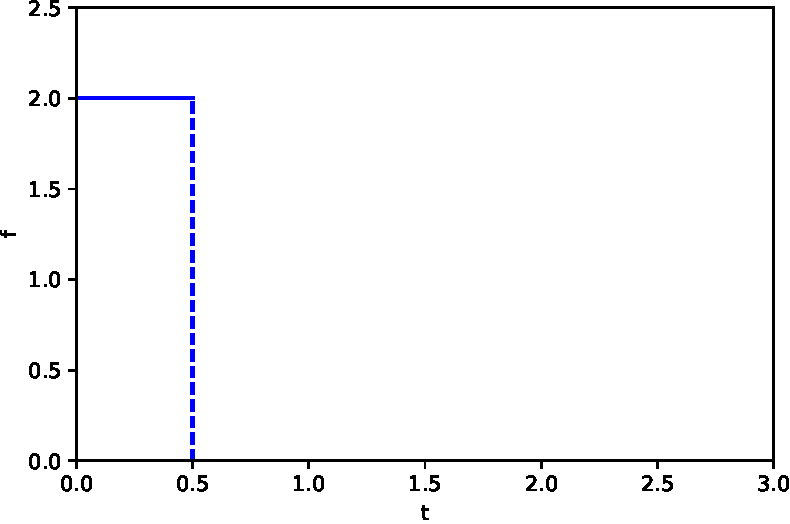
\includegraphics[width=0.5\textwidth]{ImpulseEg.pdf}
	\caption{The function $f_a(t)$ used in the check, taking $a=\frac12$.}
	\label{fig:impulseeg}
\end{figure}

Applying the Laplace transform to both sides:
\begin{align*}
	s^2Y + Y &= \frac{1}{a}\left(\frac{1}{s} - \frac{e^{-as}}{s}\right) \\
	Y(s) &= \frac{1-e^{-as}}{as(s^2+1)} = G(s)(1-e^{-as}),
\end{align*}
where
\begin{align*}
	G(s) &= \frac{1}{as(s^2+1)} = \frac{1}{a} \left(\frac{1}{s} - \frac{s}{s^2+1}\right) \\
	\implies g(t) &= \frac{1}{a} \left(u_0(t) - \cos(t)u_0(t)\right).
\end{align*}
Note that the $u_0(t)$ terms are introduced to ensure that $g(t)$ (and therefore $y(t)$) is zero for $t<0$. Therefore
\begin{align*}
	y(t) &= \frac{1}{a} \left(u_0(t)(1-\cos(t)) - u_a(t)(1-\cos(t-a))\right) \\
	&= \begin{cases}0 & \text{if }t<0 \\ \frac{1}{a}(1-\cos(t)) & \text{if } 0 \leq t \leq a \\ \frac{1}{a}(\cos(t-a)-\cos(t)) & \text{if } t>a \end{cases}.
\end{align*}
Taking the limit as $a \to 0$
\[
\frac{1}{a}(\cos(t-a)-\cos(t)) = \frac{1}{a}(\cos{t}\cos{a} + \sin{t}\sin{a} - \cos{t}) \to \sin{t}
\]
Therefore
\[
y(t) = \begin{cases}0 & \text{if } t<0 \\ \sin{t} & \text{if } t>a>0 \end{cases}.
\]

This is what we find by first solving the differential equation then taking the limit of this solution as $a \to 0$. Now we do this the other way around: taking the limit then solving:
\begin{align*}
	y'' + y &= \delta(t) \\
	s^2Y + Y &= 1 \\
	Y(s) &= \frac{1}{s^2+1} \\
	\implies y(t) &= \sin{t}.
\end{align*}
This is of course the same result - this direction of calculation is much faster and more convenient.

\begin{eg}
	We solve the ODE
	\[
	2y''+y'+2y=\delta(t-5) \quad\text{with}\quad y(0)=y'(0)=0.
	\]
	Applying the Laplace transform:
	\[
	2s^2Y + sY + 2Y = e^{-5s}.
	\]
	Therefore
	\begin{align*}
		Y(s) &= \frac{e^{-5s}}{2s^2+s+2} = \frac12 \frac{e^{-5s}}{(s+\sfrac14)^2+\sfrac{15}{16}} \\
		&= \frac12 e^{-5s} \frac{4}{\sqrt{15}} \frac{\sqrt{15}/4}{(s+\sfrac14)^2+\sfrac{15}{16}}.
	\end{align*}
	Recognising that the final fraction is the Laplace transform of $e^{-t/4}\sin\left(\frac{\sqrt{15}}{4}t\right)$ (see \Cref{table:laplace}) we invert the transform (also dealing with the $e^{-5s}$ by inverting an s-shift) and find that
	\begin{align*}
		y(t) &= \frac12 \frac{4}{\sqrt{15}} e^{-(t-5)/4} \sin\left(\frac{\sqrt{15}}{4}(t-5)\right) u_5(t) \\
		&= \frac{2}{\sqrt{15}} e^{-(t-5)/4} \sin\left(\frac{\sqrt{15}}{4}(t-5)\right) u_5(t)
	\end{align*}
\end{eg}


\subsection{Convolution of Two Functions}

The convolution of two functions $f(t)$ and $g(t)$ is given by:
\begin{equation}
	(f * g)(t) = \int_0^t f(\tau)g(t - \tau) \,d\tau = \int_0^t f(t - \tau)g(\tau) \,d\tau.
\end{equation}

Properties of Convolution:
\begin{enumerate}
	\item Distributive: $f*(g+h) = (f*g)+(f*h)$.
	\item Commutative: $f*g = g*f$.
	\item Associative: $f*(g*h) = (f*g)*h$.
\end{enumerate}

\begin{proof}\hfill
	\begin{enumerate}
		\item The distributive property follows easily from the definition and linearity of the integral.
		\item To prove the commutative property, begin with the definition of the convolution:
		\[
		(f*g)(t) = \int_0^t f(\tau) g(t-\tau) \,d\tau.
		\]
		We make a change of variables $\tau' = t - \tau$. Changing the constants of integration,
		\[
		(f*g)(t) = \int_0^t f(t - \tau') g(\tau) \,d\tau' = (g*f)(t)
		\]
		\item To prove the associative property:
		\begin{align*}
			f*(g*h) & = \int_0^t f(\tau) \,d\tau \int_0^{t-\tau '} h(\tau') g(t - \tau - \tau ') \,d\tau' \\
			& = \int_0^{t} h(\tau')\,d\tau' \int_0^{t-\tau'} f(\tau) g(t - \tau - \tau ') \,d\tau \\
			& = h*(f*g) = (f*g)*h,
		\end{align*}
		where $h*(f*g) = (f*g)*h$ follows since we have already proved commutativity.
	\end{enumerate}
\end{proof}

\subsubsection{Convolution Theorem}

\begin{theorem}[Convolution theorem]
	If $F(s) = \Lap{f(t)}$ and $G(s) = \Lap{g(t)}$ both exist for $s > a \geq 0$, then
	\[
	H(s) = F(s)G(s) = \Lap{f*g}.
	\]
	In other words, the Laplace transform of the convolution is the product of the Laplace transforms for the individual functions.
\end{theorem}

\begin{proof}
	From the definition of the convolution and Laplace transform, we have
	\begin{align*}
		\Lap{(f*g)}(s) &= \int_0^{\infty} e^{-st}\,dt \int_0^t f(\tau)g(t-\tau)\,d\tau.
		\intertext{By changing the ranges of integration:}
		&= \int_0^{\infty} f(\tau) \,d\tau \int_{\tau}^{\infty} e^{-st} g(t-\tau) \,dt 
		\intertext{Making a change of variables $t-\tau = \tau'$:}
		&= \int_0^{\infty} f(\tau) \,d\tau \int_0^{\infty} e^{-s(\tau' + \tau)}g(\tau') \,d\tau' \\
		&= \int_0^{\infty} f(\tau)e^{-s\tau}\,d\tau \int_0^{\infty} e^{-s\tau'}g(\tau')\,d\tau'\\
		&= \Lap{f} \Lap{g}
	\end{align*}
\end{proof}

This theorem is useful for inverting Laplace transforms, since
\[
\Lapinv{F(s)G(s)} = (f*g)(t).
\]

\subsubsection{Application to Second-Order ODEs}

\begin{eg}
	We solve the ODE
	\[
	y'' + \omega^2y = f(t) \quad\text{with}\quad y(0) = y'(0) = 0.
	\]
	Applying the Laplace transform to both sides of the equation,
	\begin{align*}
		s^2Y(s) + \omega^2Y(s) = F(s) = \Lap{f}(s) \\
		Y(s) = \frac{F(s)}{s^2+\omega^2} = F(s) \frac{1}{s^2 + \omega^2}.
	\end{align*}
	If we apply the inverse Laplace transform to:
	\begin{itemize}
		\item From $F(s)$, we get $f(t)$. 
		\item From $\frac{1}{s^2+\omega^2}$, we get $\frac{1}{\omega} \sin(\omega t)$.
	\end{itemize}
	So
	\[
	y(t) = \frac{1}{\omega} \int_0^t f(\tau)\sin\left(\omega(t-\tau)\right) \,d\tau.
	\]
\end{eg}

We can also use the Convolution theorem to find a general procedure for solving second-order ODEs. Consider the second-order ODE
\[
	ay'' + by' + cy = f(t) \quad\text{with}\quad y(0) = y_0, \,\, y'(0) = y_0'.
\]
Applying the Laplace transform, we have
\begin{align*}
	a(s^2Y - sy_0 - y_0') + b(sY-y_0)+cY &= F(s) \\
	\implies (as^2+bs+c)Y(s) &= F(s) + (as+b)y_0 + ay_0' \\
	\implies Y(s) &= \frac{1}{as^2+bs+c} \left(F(s) + G(s)\right) \\
	\implies Y(s) &= H(s)\left(F(s)+G(s)\right),
\end{align*}
where $H(s) = \frac{1}{as^2+bs+c}$, and $G(s) = (as+b)y_0 + ay_0'$.

Okay, so let's take a trip to the Laplace world now! For $Y$, the response to forcing and to initial conditions is split into 2 parts:
\begin{itemize}
	\item $F(s)$ is a response from forcing.
	\item $G(s)$ is a response that depends on the initial conditions. 
	\item $H(s)$ helps transfer these into the solution $Y$ so (surprise surprise!) $H(s)$ is called a transfer function.
\end{itemize}

By the convolution theorem, if we have the inverse Laplace transforms of $F$, $G$, and $H$ then we can find the solution $y(t)$ as:
\[
y(t) = \int_0^t h(t-\tau)f(\tau) \,d\tau + \int_0^t h(t-\tau)g(\tau)\,d\tau.
\]

\underline{Transfer Function}:
\[
H(s) = \frac{1}{as^2+bs+c}
\]
has a Laplace inverse given by $\Lapinv{H} = h(t)$, where 
\[
ah'' + bh' + ch = \delta(t), \quad\text{with}\quad h(0) = h'(0) = 0,
\]
where $\delta(t)$ is a Dirac distribution. So $h(t)$ is a solution to a differential equation where the forcing is just a distribution.

Thus, you can write the solution to any differential equation with constant coefficients as the sum of two convolutions, one relating to the forcing function $f(t)$, and the other relating to the initial conditions.

\begin{eg}
	We solve the ODE
	\[
	y''+4y = f(t) \quad\text{with}\quad y(0) = 3, \,\, y'(0) = 1.
	\]
	Applying the Laplace transform:
	\begin{align*}
		s^2Y - 3s - 1 + 4Y &= F(s) \\
		\implies (s^2+4)Y &= F(s)+3s+1 \\
		\implies Y(s) &= H(s) \left[ F(s) + 3s+1\right] \quad \text{where } H(s) = \frac{1}{s^2+4}.
	\end{align*}
	Applying the inverse Laplace transform to $H(s)$:
	\[
	h(t) = \frac12 \sin{2t}.
	\]
	Therefore
	\begin{align*}
		Y(s) &= H(s)F(s) + \frac{3s}{s^2+4} + \frac{1}{s^2+4} \\
		\implies y(t) &= \frac12 \int_0^t \sin\left(2(t-\tau)\right) f(\tau) \,d\tau + 3\cos{2t} + \frac12\sin{2t}.
	\end{align*}
\end{eg}

\subsubsection{Integral Equations}

We can use convolutions to solve integral equations; that is, equations in which a function $y(t)$ appears inside an integral. This is best illustrated by an example.

\begin{eg}
	We solve the integral equation
	\[
	y(t) = \int_0^t \cos{(t-\tau)}y(\tau)\,d\tau + 1.
	\]
	The RHS of the above equation is a convolution, so take Laplace transform on both sides 
	\begin{align*}
		Y(s) &= \frac{s}{s^2+1}Y(s) + \frac1s \\
		\implies \frac{s^2-s+1}{s^2+1}Y(s) &= \frac1s \\
		\implies Y(s) &= \frac{1+s^2}{s(s^2-s+1)} = \frac{s^2-s+1}{s(s^2-s+1)} + \frac{s}{s(s^2-s+1)} \\
		&= \frac1s + \frac{1}{s^2-s+1} = \frac1s + \frac{\sqrt{3}/2}{\left(s-1/2\right)^2 + 3/4} \cdot \frac{2}{\sqrt{3}}.
	\end{align*}
	Finally, we take the inverse Laplace transform of each of these terms:
	\[
	y(t) = 1 + \frac{2}{\sqrt{3}}e^{-t/2} \sin{\left(\frac{\sqrt{3}t}{2}\right)}.
	\]
\end{eg}

\begin{eg}
	Show that
	\[
		\phi(t) = \int_0^t \int_0^{t_1} \cdots \int_0^{t_{n-1}} f(t) dt_1 dt_2 \cdots dt_n = \int_0^t \frac{(t-\tau)^{n-1}}{(n-1)!} f(\tau)\,d\tau.
	\]
	First, notice that
	\[
		\Lapb{\int_0^t f(\tau)\,d\tau} = \Lapb{\int_0^t f(\tau) u_0(t-\tau) \,d\tau} =  \Lap{f*u_0} = \Lap{f}\Lap{u_0} = \frac{F(s)}{s}.
	\]
	Applying this property recursively, we find that
	\[
		\Lap{\phi} = \frac{F(s)}{s^n}.
	\]
	Then
	\[
		\Lapinvb{\frac{1}{s^n}} = \frac{t^{n-1}}{(n-1)!} \quad\text{since}\quad \Lap{t^n} = \frac{n!}{s^{n+1}}.
	\]
	Therefore, by the Convolution theorem,
	\[
		\Lap{\phi} = \Lapb{\frac{t^{n-1}}{(n-1)!}}\Lap{f(t)} = \Lapb{\int_0^t \frac{(t-\tau)^{n-1}}{(n-1)!} f(\tau)\,d\tau},
	\]
	and taking the inverse Laplace transform yields
	\[
		\phi(t) = \int_0^t \frac{(t-\tau)^{n-1}}{(n-1)!} f(\tau)\,d\tau.
	\]
\end{eg}

The Laplace transform can also be used to solve linear systems of ODEs.

\begin{eg}
	Solve the system of initial value problems
	\begin{align*}
		x'(t) - 2y(t) &= 4t, \quad x(0)=4 \\
		y'(t) + 2y(t) - 4x(t) &= -4t-2, \quad y(0)=-5
	\end{align*}
	Taking the Laplace transforms of both ODEs yields
	\begin{align*}
		sX(x) - 4 - 2Y(s) &= \frac{4}{s^2} \\
		sY(s) + 5 + 2Y(s) - 4X(s) &= -\frac{4}{s^2} - \frac{2}{s},
	\end{align*}
	where $X(s) = \Lap{x(t)}$ and $Y(s) = \Lap{y(t)}$.
	
	Solving the pair of transformed ODEs for $X(s)$, we find
	\[
		(s(s+2)-8)X(s) = \frac{(s+2)(4s^2+4)}{s^2} - \frac{10s^2+4s+8}{s^2},
	\]
	which simplifies to
	\[
		X(s) = \frac{4s-2}{(s+4)(s+2)} = \frac{3}{s+4} + \frac{1}{s-2}.
	\]
	Applying the inverse Laplace transform yields
	\[
		x(t) = 3e^{-4t} + e^{2t}.
	\]
	Then, rearranging the first ODE yields
	\[
		y(t) = \frac12 x'(t) - 2t = -6e^{-4t} + e^{2t} - 2t.
	\]
\end{eg}

\begin{exercise}
	The system of initial value problems in the above example can be written in matrix form as
	\[
		\xtp = \mat{0 & 2 \\ 4 & -2}\xt + \mat{4t \\ -4t - 2}, \quad \vbx(0) = \mat{4 \\ -5}.
	\]
	Using the methods of \Cref{sec:firstorder}, solve this system and confirm that the result is equivalent to the solution obtained using the Laplace transform.
\end{exercise}

\pagebreak
\subsection{Table of Elementary Transforms}\label{sec:laptable}

\begin{table}[!ht]
	\begin{center}
		\begin{tabular}{>{$}c<{$}|>{$}c<{$}}
			f(t) = \Lapinv{F(s)} & F(s) = \Lap{f(t)} \\
			\hline
			1 & \dfrac{1}{s}, \quad s>0 \rule{0pt}{1.8em}\\[1em]
			e^{at} & \dfrac{1}{s-a}, \quad s>0 \\[1em]
			t^n, \quad n \in \mathbb{N} & \dfrac{n!}{s^{n+1}}, \quad s>0 \\[1em]
			t^p, \quad p>-1 & \dfrac{\Gamma(p+1)}{s^{p+1}}, \quad s>0 \\[1em]
			\sin(at) & \dfrac{a}{s^2+a^2}, \quad s>0 \\[1em]
			\cos(at) & \dfrac{s}{s^2+a^2}, \quad s>0 \\[1em]
			\sinh(at) & \dfrac{a}{s^2-a^2} \quad s>|a| \\[1em]
			\cosh(at) & \dfrac{s}{s^2-a^2} \quad s>|a| \\[1em]
			e^{at}\sin(bt) & \dfrac{b}{(s-a)^2+b^2}, \quad s>a \\[1em]
			e^{at}\cos(bt) & \dfrac{s-a}{(s-a)^2+b^2}, \quad s>a \\[1em]
			t^ne^{at}, \quad n\in\mathbb{N} & \dfrac{n!}{(s-a)^{n+1}}, \quad s>a \\[1em]
			u_c(t) = \begin{cases}0 & t<c \\ 1 & t\geq c\end{cases} & \dfrac{e^{-cs}}{s}, \quad s>0 \\[1em]
			u_c(t)f(t-c) & e^{-cs}F(s) \\[1em]
			e^{-ct}f(t) & F(s+c) \\[1em]
			tf(t) & -\dfrac{d}{ds}F(s) \\[1em]
			(-t)^nf(t) & F^{(n)}(s) \\[1em]
			f(ct) & \dfrac{1}{c}F\left(\dfrac{s}{c}\right), \quad c>0 \\[1em]
			\delta(t-c) & e^{-cs} \\[1em]
			\delta(t-c)f(t) & e^{-cs}f(c) \\[1em]
			f^{(n)}(t) & s^nF(s) - s^{n-1}f(0) - \cdots - f^{(n-1)}(0) \\[1em]
			(f*g)(t) = \int_0^t f(\tau)g(t-\tau)\,d\tau & F(s)G(s)
		\end{tabular}
	\end{center}
	\caption{Elementary Laplace Transforms.}
	\label{table:laplace}
\end{table}


\begin{thebibliography}{9}
	\addcontentsline{toc}{section}{References}
	\bibitem{boyce}
	Boyce, William E. (2017). ``Boyce's Elementary Differential Equations and Boundary Value Problems.'' Wiley-Blackwell. ISBN: 9781119382874.
	
	\bibitem{numgraph}
	Mohanta, Rishika and Assisi, Collins (2019). ``Parallel scalable simulations of biological neural networks using TensorFlow: A beginner's guide.'' URL: \url{https://arxiv.org/abs/1906.03958v1}.
	
	\bibitem{limitcycles}
	Sun, X. and Lei, J. (2013). ``Limit Cycle.'' In: Dubitzky, W., Wolkenhauer, O., Cho, K. H., and Yokota, H. (eds) ``Encyclopedia of Systems Biology.'' Springer, New York, NY. URL: \url{https://doi.org/10.1007/978-1-4419-9863-7_533}.
	
	\bibitem{olver}
	Olver, F. W. J. (1972). ``Chapter 9. Bessel Functions of Integer Order'' In: Abramowitz, Milton and Stegun, Irene Ann, (eds) ``Handbook of Mathematical Functions with Formulas, Graphs, and Mathematical Tables.'' p. 361. Dover Publications. ISBN 9780486612720. URL: \url{https://personal.math.ubc.ca/~cbm/aands/page_361.htm}.
	
	\bibitem{watson}
	Whittaker, E. and Watson, G. (1996). ``Bessel Functions.'' In ``A Course of Modern Analysis.'' pp. 355-385. Cambridge: Cambridge University Press. URL: \url{https://doi.org/10.1017/CBO9780511608759.018}.
\end{thebibliography}

\end{document}